\documentclass%
%[handout]
{beamer}
% % % % % % % %
% % % % % % % %
% % % % % % % %
%IMPORTANT
%compiles with
%pdflatex -shell-escape
%IMPORTANT
% % % % % % % %
% % % % % % % %
% % % % % % % %
\mode<presentation>
{
\useinnertheme{rounded}
\useoutertheme{infolines}
\usecolortheme{orchid}
\usecolortheme{whale}
}

\usepackage[english]{babel}
\usepackage[latin1]{inputenc}
\usepackage[all,cmtip]{xy}
\usepackage{times}
\usepackage[T1]{fontenc}
\usepackage{../example-templates}
\usepackage{../pstricks-commands}

\usepackage{auto-pst-pdf}
\usepackage{pst-plot}
%\usepackage{pstricks-add}

% Or whatever. Note that the encoding and the font should match. If T1
% does not look nice, try deleting the line with the fontenc.


\graphicspath{{../../modules/}}

\newtheoremstyle{partialproof}{3pt}{3pt}{}{}{}{.}{.5em}{}
\theoremstyle{partialproof} \newtheorem{partialproof}[theorem]{Proof.}
%\DeclareMathOperator{\diff}{d}
\setbeamertemplate{navigation symbols}{}

\includeonlylecture{1}

\newcommand{\lect}[3]{
  \date{#1}
  \lecture[#1]{#2}{#3}
}

\setbeamertemplate{footline}
{
  \leavevmode%
  \hbox{%
  \begin{beamercolorbox}[wd=.333333\paperwidth,ht=2.25ex,dp=1ex,center]{author in head/foot}%
    \usebeamerfont{author in head/foot}\insertshortauthor
  \end{beamercolorbox}%
  \begin{beamercolorbox}[wd=.333333\paperwidth,ht=2.25ex,dp=1ex,center]{title in head/foot}%
    \usebeamerfont{title in head/foot}\insertshorttitle
  \end{beamercolorbox}%
  \begin{beamercolorbox}[wd=.333333\paperwidth,ht=2.25ex,dp=1ex,center]{date in head/foot}%
    \usebeamerfont{date in head/foot}\insertshortdate{}
  \end{beamercolorbox}}%
  \vskip0pt%
}

% If you have a file called "university-logo-filename.xxx", where xxx
% is a graphic format that can be processed by latex or pdflatex,
% resp., then you can add a logo as follows:

%\pgfdeclareimage[height=0.8cm]{logo}{bluelogo}
%\logo{\pgfuseimage{logo}}
\renewcommand{\Arcsin}{\arcsin}
\renewcommand{\Arccos}{\arccos}
\renewcommand{\Arctan}{\arctan}
\renewcommand{\Arccot}{\text{arccot\hspace{0.03cm}}}
\renewcommand{\Arcsec}{\text{arcsec\hspace{0.03cm}}}
\renewcommand{\Arccsc}{\text{arccsc\hspace{0.03cm}}}

\begin{document}

\AtBeginLecture{%

\title[\insertlecture]{FreeCalc}
\subtitle{\insertlecture}
\author[FreeCalc]{}
\institute[UMass Boston]{University of Massachusetts Boston}
\date{\insertshortlecture}
\begin{frame}
  \titlepage
\end{frame}
}%

% begin lecture
\lect{\today}{Sample}{1}{
%\begin{frame}
 \frametitle{Main Questions}


\begin{columns}[t]
\column[T]{0.4\textwidth}

\begin{pspicture}(-1,-2)(2,2)
\renewcommand{\fcScreen}{[-2 -1 -0.55] 0}
\tiny
\fcBoundingBox{-1}{-2}{2}{2}
\fcParallelogramIIId{[2 2 0]}{[1 2 -1]}{[1 2 2]}
\fcAxesIIId{2}{2}{2}
\fcLineIIId[arrows=->]{[ 0 0 0]}{[1 1 1]}
\fcDotIIId{[1 1 1]}
\fcPutIIId[lb]{[1 1 1]}{$~~Q(x,y,z)$}
\fcLineIIId{[0.6 0.95 0.35]}{[1.4 1.05 1.65]}

\fcLineIIId[arrows=->]{[ 0 0 0]}{[1 2 0.5]}
\fcDotIIId{[1 2 0.5]}
\fcPutIIId[lb]{[1 2 0.5]}{$~~P(x,y,z)$}
\end{pspicture}

\column{0.6\textwidth}
What condition(s) should
\begin{itemize}
\item the position vector
\item the coordinates
\end{itemize}

of a point satisfy for it to be on a specific

\begin{itemize}
\item line $L$
\item plane $\mathcal{P}$?
\end{itemize}
\end{columns}

Condition(s) in terms of:
\begin{itemize}
\item position vector $\Rightarrow$ vector (system of) equations;
\item coordinates $\Rightarrow$ scalar equations.
\end{itemize}
\end{frame}

%\begin{frame}
 \frametitle{Line from Two Points}

\begin{columns}

\column{0.4\textwidth}
\psset{xunit=1.4cm, yunit=1.4cm}
\begin{pspicture}(-1,-0.4)(2,2.1)
\fcBoundingBox{-0.8}{-0.4}{4}{2.1}
\renewcommand{\fcScreen}{[-3 -1 -0.2] 0}
\tiny
\uncover<5->{\fcAxesIIId{2}{2}{2}}
\fcLineIIId{[0.5 0.5 1]}{[3 3 0.5]}
\fcLineIIId{[0.5 0.5 1]}{[4 4 0.3]}
\fcLineIIId[arrows=->]{[0 0 0]}{[1 1 0.9]}
\fcPutIIId[br]{[0.5 0.5 0.45]}{$\fcv r_0~$}

\fcLineIIId[linecolor=blue, arrows=->]{[1 1 0.9]}{[2.5 2.5 0.6]}
\fcPutIIId[br]{[1.75 1.75 0.8]}{$\fcv u$}

\fcLineIIId[arrows=->]{[0 0 0]}{[2.5 2.5 0.6]}
\fcPutIIId[b]{[1.25 1.25 0.3]}{$\fcv r_1$}

\fcDotIIId{[1 1 0.9]}
\fcPutIIId[lb]{[1 1 0.95]}{$P_0\uncover<5->{(x_0,y_0, z_0)} $}
\fcDotIIId{[2.5 2.5 0.6]}
\fcPutIIId[lb]{[2.5 2.5 0.65]}{$P_1\uncover<5->{(x_1, y_1, z_1)}$}
\fcDotIIId{[3.5 3.5 0.4]}
\fcLineIIId[arrows=->]{[0 0 0]}{[3.5 3.5 0.4]}
\fcPutIIId[b]{[1.75 1.75 0.2]}{$\fcv r$}
\fcPutIIId[b]{[3.5 3.5 0.5]}{$~P(x,y,z)$}
\fcPutIIId[t]{[4 4 0.3]}{$~L$}
\fcPutIIId[r]{[0 0 0.1]}{$O~~$}
\end{pspicture}
\column{0.6\textwidth}
\begin{itemize}
\item Given: distinct points $P_0$ and $P_1$, position vectors $\textbf{r}_0$ and $\textbf{r}_1$.
\item Goal: write equations of line $L$ through $P_0$ and $P_1$.
\item<2-> Direction of $L$: $\textbf{u} = \textbf{r}_1 - \textbf{r}_0$.
\item<5-> $\fcv{u} = \langle x_1-x_0,y_1-y_0,z_1-z_0\rangle$
\end{itemize}. 
\end{columns}
\uncover<3->{
\begin{definition}
\alert<1->{Parametric vectorial equation} of a line $L$:\\
$
\textbf{r} = \textbf{r}_0 + t(\textbf{r}_1-\textbf{r}_0)
\quad \Leftrightarrow \quad   \textbf{r} = (1-t)\textbf{r}_0 + t\textbf{r}_1
$

\uncover<5->{
\alert<1->{Parametric scalar equations} of a line $L$:
$\left|
\begin{array}{ll}
x & = x_0 + t(x_1-x_0) \\
y & = y_0 + t(y_1-y_0) \\
z & = z_0 + t(z_1-z_0)
\end{array}
\right. \Leftrightarrow \left| \begin{array}{ll}
x & = (1-t)x_0 + tx_1 \\
y & = (1-t)y_0 + ty_1 \\
z & = (1-t)z_0 + tz_1
\end{array}
\right. , \quad t \text{ real number.}$
} %uncover
\end{definition}
} %uncover
\end{frame}
%%\begin{comment}
\begin{frame}
\frametitle{Rectangular/Cartesian Coordinates}
\begin{columns}
\column[t]{0.3\textwidth}
\psset{xunit=0.7cm, yunit=0.7cm}
\begin{pspicture}(-0.5 ,-2)(4.5, 4)
\fcBoundingBox{-0.5}{-2}{4.5}{4}
\tiny
\uncover<3->{
\fcLineIIId{[0 0 0]}{[3 0 0]}
\fcLineIIId{[0 0 0]}{[0 3 0]}
\fcLineIIId{[0 0 0]}{[0 0 3]}
}
\uncover<4->{
\fcLineIIId[arrows=->]{[0 0 0]}{[3 0 0]}
\fcLineIIId[arrows=->]{[0 0 0]}{[0 3 0]}
\fcLineIIId[arrows=->]{[0 0 0]}{[0 0 3]}
}
\uncover<5->{
\fcPutIIId[t]{[3 0 0]}{\alertNoH{5}{$x$}}
\fcPutIIId[lb]{[0 3 0]}{\alertNoH{5}{$y$}}
\fcPutIIId[b]{[0 0 3]}{\alertNoH{5}{$z$}}
}
\uncover<2->{ %
\fcPutIIId[r]{[0 0 0]}{$O~~~$} %
\fcDotIIId[linecolor=black]{[0 0 0]} %
}
\end{pspicture}


\vfill
\column{0.7\textwidth}
\begin{itemize}
\item<1-> A Cartesian coordinate system is given by fixing:
\begin{itemize}
\item<2-> a point $O$ (called the origin),
\item<3-> 3 pairwise perpendicular lines intersecting at the origin,
\item<4-> a direction in each of the coordinate axis.
\end{itemize}
\item<5-> The three lines are labeled as $x$-axis, $y$-axis and $z$-axis.
\end{itemize}

\vskip 3cm
\end{columns}


%
\end{frame}

\begin{frame}
\frametitle{Rectangular/Cartesian Coordinates}
\begin{columns}
\column[t]{0.3\textwidth}
\psset{xunit=0.7cm, yunit=0.7cm}
\begin{pspicture}(-0.5 ,-2)(4.5, 4)
\fcBoundingBox{-0.5}{-2}{4.5}{4}
\tiny
\renewcommand{\fcScreen}{[-1 1.1 -0.5] 0}
\fcAxesIIId{3}{3}{3}
\fcPutIIId[r]{[0 0 0]}{$O~$}
\fcPutIIId[b]{[2.5 2.5 2.8]}{$P(x_P,y_P,z_P)$}
\uncover<9->{
\fcLineIIId[linecolor=gray]{[2.5 2.5 2.5]}{[2.5 2.5 0]}
\fcLineIIId[linecolor=gray]{[2.5 2.5 2.5]}{[2.5 0 2.5]}
\fcLineIIId[linecolor=gray]{[2.5 2.5 2.5]}{[0 2.5 2.5]}
\fcLineIIId[linecolor=gray]{[0 2.5 2.5]}{[0 0 2.5]}
\fcLineIIId[linestyle=dashed, linecolor=gray]{[0 2.5 2.5]}{[0 2.5 0]}
\fcLineIIId[linecolor=gray]{[2.5 0 2.5]}{[0 0 2.5]}
\fcLineIIId[linecolor=gray]{[2.5 0 2.5]}{[2.5 0 0]}
\fcLineIIId[linestyle=dashed, linecolor=gray]{[2.5 2.5 0]}{[0 2.5 0]}
\fcLineIIId[linecolor=gray]{[2.5 2.5 0]}{[2.5 0 0]}%
}%
\fcDotIIId{[2.5 2.5 2.5]}%
\uncover<3-8>{%
\fcPerpendicularIIId{[2.5 2.5 2.5]}{[1 0 0]}{0.3}%
\fcPutIIId[t]{[2.5 0 -0.1]}{$Q$}%
}%
\uncover<4->{\fcPutIIId[t]{[1.25 0 -0.1]}{$x_P$}}%
\uncover<6-8>{%
\fcPerpendicularIIId{[2.5 2.5 2.5]}{[0 1 0]}{0.3}%
\fcPerpendicularIIId{[2.5 2.5 2.5]}{[0 0 1]}{0.3}%
}%
\uncover<6->{%
\fcPutIIId[b]{[0 1.25 0.1]}{$y_P$}%
\fcPutIIId[r]{[0 0 1.25]}{$z_P~~$}%
}
\end{pspicture}


\vfill
\column{0.7\textwidth}
\begin{itemize}
\item<1-> $P$ -point. We assign to it triple $(x_P,y_P,z_P)$.
\item<2-> Assignment will be such that distinct points are assigned distinct triples.
\item<3-> $Q=$ base of perpendicular from $P$ to $x$-axis.
\item<4-> Define $x_P$ as \alertNoH{5}{signed distance b-n $O$ and $Q$}.
\item<5-> Take distance with \alertNoH{5}{$+$ sign if $OQ$ points in direction of $x$-axis, $-$ sign else}.
\item<6-> Definitions of $y_P$, $z_P$ are similar.
\item<7-> $(x_P,y_P,z_P)$ = Cartesian coordinates of $P$. 
\item<8-> $x_P$ is called the $x$-coordinate of $P$,  and so on for other axes.
\item<9-> $(x_P, y_P, z_P)$ = singed lengths of edges of the rectangular box indicated in the picture.
\end{itemize}

\vfill
\end{columns}

\vskip 5cm

\end{frame}
%\end{comment}

%\begin{frame}
\frametitle{$\fcv{orth}_{\fcv u}$ is a linear operator}
\begin{theorem}
$\alert<14>{ \alert<13>{ \fcv{orth}_{\fcv u}(\alert<12>{ \fcv v_1 +\fcv v_2}) }= \alert<10>{ \fcv{orth}_{\fcv u} \fcv v_1 } +\alert<11>{\fcv{orth}_{\fcv u} \fcv v_2}}$
\end{theorem}
\begin{proof}
\begin{columns}
\column{0.3\textwidth}
Geometric proof:
\uncover<8->{
\psset{xunit=0.9cm, yunit=0.9cm}
\begin{pspicture}(-0.5,-0.7)(3.8,4.2)%
\tiny%
\fcBoundingBox{-0.5}{-0.7}{3.8}{4.2}%
\uncover<9->{%
\fcParallelogramIIId{[0 -0.5 -0.5]}{[0 3 0]}{[0 0 3]}%
\fcPutIIId[lt]{[0.3 3 3]}{$\mathcal P$}%
}%
\fcLineIIId[arrows=->]{[0 0 0]}{[1 0 0]}%
\fcPutIIId[t]{[0.5 0 -0.1]}{$\fcv u$}%
\uncover<10->{%
\fcPerpendicularIIId{[1 1 2]}{[0 1 2]}{0.2}%
}%
\fcLineIIId[arrows=->]{[0 0 0]}{[1 1 2]}%
\fcPutIIId[tl]{[0.5 0.5 1]}{$\fcv v_1$}%
\uncover<10->{%
\fcLineIIId[linecolor=blue, arrows=->]{[0 0 0]}{[0 1 2]}%
\fcPutIIId[rb]{[0 0.5 1]}{$\color{blue}{\alert<14>{ \fcv{orth}_{\fcv u } \fcv v_1}}$}%
}%
\uncover<11->{\fcPerpendicularIIId{[1 2 0]}{[0 2 0]}{0.2}}%
\fcLineIIId[arrows=->]{[0 0 0]}{[1 2 0]}%
\fcPutIIId[t]{[0.5 1 -0.1]}{$\fcv v_2$}%
\uncover<11->{\fcLineIIId[linecolor=blue, arrows=->]{[0 0 0]}{[0 2 0]}}%
\uncover<11->{%
\fcLineIIId[arrows=->]{[1 1 2]}{[2 3 2]}%
\fcPutIIId[b]{[1.5 2 2]}{$\fcv v_2$}%
}%
\uncover<11->{%
\fcPerpendicularIIId{[2 3 2]}{[0 3 2]}{0.2}%
}%
\uncover<11->{%
\fcLineIIId[arrows=->, linecolor=blue]{[0 1 2]}{[0 3 2]}%
\fcPutIIId[b]{[0 2 2.2]}{$\color{blue}{\alert<14>{ \fcv{orth}_{\fcv u} \fcv v_2} }$}%
}%
\uncover<13->{%
\fcLineIIId[arrows=->, linecolor=blue]{[0 0 0]}{[0 3 2]}%
\fcPutIIId[l]{[0 2 1.3]}{$\color{blue}{\alert<14>{ \fcv{orth}_{\fcv u} (\fcv v_1 +\fcv v_2)}}$}%
}%
\uncover<12->{%
\fcLineIIId[arrows=->]{[0 0 0]}{[2 3 2]}%
\fcPutIIId[lt]{[1 1.5 1]}{$\fcv v_1 +\fcv v_2$}%
}%
\uncover<14>{%
\fcLineIIId[linewidth=1.5pt, arrows=->, linecolor=red]{[0 0 0]}{[0 3 2]}%
\fcLineIIId[linewidth=1.5pt, arrows=->, linecolor=red]{[0 1 2]}{[0 3 2]}%
\fcLineIIId[linewidth=1.5pt, arrows=->, linecolor=red]{[0 0 0]}{[0 1 2]}%
}%
\end{pspicture}
\uncover<9->{\alert<9>{Let $\mathcal P$: plane $\perp \fcv u$.}}
} %uncover
\column{0.7\textwidth}
Algebraic proof:

\small
\noindent \uncover<2->{
$
\begin{array}{r@{~}c@{~}l}
\fcv{orth}_{\fcv u}(\fcv v_1+\fcv v_2)&=& (\fcv v_1+\fcv v_2)- \alert<3>{\fcv{proj}_{\fcv u}(\fcv v_1 +\fcv v_2)}\\
\uncover<3->{&=&(\alert<4>{\fcv v_1}+\alert<5>{\fcv v_2})\alert<4,5>{-} \left(\alert<3>{ \alert<4>{\fcv{proj}_{\fcv u}(\fcv v_1)} +\alert<5>{\fcv{proj}_{\fcv u}(\fcv v_2)}}\right)} \\
\uncover<4->{&=&\left(\alert<4,6>{\fcv v_1- \fcv{proj}_{\fcv u}(\fcv v_1)}\right)+\left(\alert<5,7>{\fcv v_2-\fcv{proj}_{\fcv u}(\fcv v_2)}\right)}\\
\uncover<6->{&=& \alert<6>{\fcv{orth}_{\fcv u} \fcv v_1}+\alert<7>{\fcv{orth}_{\fcv u} \fcv v_2}}
\end{array}
$
}
\normalsize
\end{columns}
\end{proof}
\end{frame}
%\begin{frame}
\frametitle{Justification of Linearity of $\times$ Product}
\begin{theorem}
$\alertNoH{11}{\fcv u\times (\fcv v_1+\fcv v_2)=\fcv u \times\fcv v_1 +\fcv u\times \fcv v_2 }$.
\end{theorem}
\begin{proof}[Geometric justification]
\begin{columns}
\column{0.41\textwidth}
\uncover<2->{%
\psset{xunit=1cm, yunit=1cm}
\begin{pspicture}(-1.5, -0.8)(3.6,4.15)
\tiny%
\fcBoundingBox{-1.5}{-0.8}{3.6}{4.15}%
\fcParallelogramIIId{[0 -1.5 -0.45]}{[0 -2.1 3.1]}{[0 3.7 0]}%
\fcPutIIId[lt]{[0.3 3 3]}{$\mathcal P$}%
\fcLineIIId[arrows=->]{[0 0 0]}{[1 0 0]}%
\fcPutIIId[t]{[0.5 0 -0.1]}{$\fcv u$}%
\uncover<1-4>{%
\fcPerpendicularIIId{[1 1 2]}{[0 1 2]}{0.2}%
\fcLineIIId[arrows=->]{[0 0 0]}{[1 1 2]}%
\fcPutIIId[tl]{[0.5 0.5 1]}{$\fcv v_1$}%
\fcPerpendicularIIId{[1 2 0]}{[0 2 0]}{0.2}%
\fcLineIIId[arrows=->]{[0 0 0]}{[1 2 0]}%
\fcPutIIId[t]{[0.5 1 -0.1]}{$\fcv v_2$}%
\fcLineIIId[linecolor=blue, arrows=->]{[0 0 0]}{[0 2 0]}%
\fcLineIIId[arrows=->]{[1 1 2]}{[2 3 2]}%
\fcPutIIId[b]{[1.5 2 2]}{$\fcv v_2$}%
\fcPerpendicularIIId{[2 3 2]}{[0 3 2]}{0.2}%
\fcLineIIId[linecolor=blue, arrows=->]{[0 0 0]}{[0 1 2]}%
\fcPutIIId[rb]{[0 0.5 1]}{$\color{blue}{ \fcv{orth}_{\fcv u } \fcv v_1}$}%
\fcLineIIId[arrows=->, linecolor=blue]{[0 1 2]}{[0 3 2]}%
\fcPutIIId[b]{[0 2 2.2]}{$\color{blue}{\fcv{orth}_{\fcv u} \fcv v_2 }$}%
\fcLineIIId[arrows=->, linecolor=blue]{[0 0 0]}{[0 3 2]}%
\fcPutIIId[l]{[0 2 1.3]}{$\color{blue}{ \fcv{orth}_{\fcv u} (\fcv v_1 +\fcv v_2)}$}%
\fcLineIIId[arrows=->]{[0 0 0]}{[2 3 2]}%
\fcPutIIId[lt]{[1 1.5 1]}{$\fcv v_1 +\fcv v_2$}%
}%uncover
\uncover<4>{%
\fcLineIIId[linewidth=1.5pt, arrows=->, linecolor=red]{[0 0 0]}{[0 1 2]}%
\fcLineIIId[linewidth=1.5pt, arrows=->, linecolor=red]{[0 1 2]}{[0 3 2]}%
\fcLineIIId[linewidth=1.5pt, arrows=->, linecolor=red]{[0 0 0]}{[0 3 2]}%
}%
\uncover<5->{%
\fcLineIIId[arrows=->]{[0 0 0]}{[0 1 2]}%
\fcLineIIId[arrows=->]{[0 1 2]}{[0 3 2]}%
\fcLineIIId[arrows=->]{[0 0 0]}{[0 3 2]}%
\fcLineIIId[arrows=->]{[0 0 0]}{[0 2 0]}%
\fcPerpendicularIIId{[1 0 0]}{[0 -1 -2]}{0.2}%
\fcPerpendicularIIId{[1 0 0]}{[0 -2 0]}{0.2}%
\fcPutIIId[rb]{[0 0.5 1]}{$\alertNoH{5}{\fcv v_1}$}%
\fcPutIIId[l]{[0 2 1.3]}{$\alertNoH{5}{\fcv v_1 +\fcv v_2}$}%
\fcPutIIId[b]{[0 2 2.2]}{$\alertNoH{5}{\fcv v_2 }$}%
\fcPutIIId[b]{[0 1 0]}{$\alertNoH{5}{\fcv v_2 }$}%
}%
\uncover<8->{\fcLineIIId[arrows=->, linecolor=blue]{[0 0 0]}{[0 -2 1]}}%
\uncover<9->{\fcLineIIId[arrows=->, linecolor=blue]{[0 0 0]}{[0 0 2]}}%
\uncover<10->{%
\fcLineIIId[arrows=->, linecolor=blue]{[0 0 0]}{[0 -2 3]}%
\fcAngleIIId[linecolor=magenta, arrows=->]{[0 3 2]}{[0 -2 3]}{0.6}%
}%
\uncover<8->{\fcAngleIIId[linecolor=orange, arrows=->]{[0 0.5 1]}{[0 -2 1]}{0.4}}%
\uncover<9->{\fcAngleIIId[linecolor=brown, arrows=->]{[0 2 0]}{[0 0 2]}{0.5}}%
\uncover<11->{%
\fcLineIIId[linewidth=1.5pt, arrows=->, linecolor=red]{[0 0 0]}{[0 -2 1]}%
\fcLineIIId[linewidth=1.5pt, arrows=->, linecolor=red]{[0 0 0]}{[0 0 2]}%
\fcLineIIId[linewidth=1.5pt, arrows=->, linecolor=red]{[0 0 0]}{[0 -2 3]}%
\fcLineIIId[linewidth=1.5pt, arrows=->, linecolor=red]{[0 0 2]}{[0 -2 3]}%
}%
\uncover<10->{\fcPutIIId[l]{[0 -1.8 2.7]}{${\fcv u \times (\fcv v_1 +\fcv v_2)}$}}%
\uncover<9->{\fcPutIIId[r]{[0 0 1]}{${\fcv u \times \fcv v_2}$}}%
\uncover<8->{\fcPutIIId[tr]{[0 -0.5 0.25]}{${\fcv u \times \fcv v_1}$}}%
\end{pspicture}
}%uncover
\column{0.59\textwidth}
\small
\uncover<2->{
$\begin{array}{r@{~}c@{~}l}
\alertNoH{4}{\fcv u\times \fcv v_1} &=& \alertNoH{4}{\fcv u\times \fcv{orth}_{\fcv u}\fcv v_1} \\
\alertNoH{4}{\fcv u\times \fcv v_2} &=&\alertNoH{4}{ \fcv u\times \fcv{orth}_{\fcv u}\fcv v_2}\\
\alertNoH{4}{\fcv u\times (\fcv v_1+\fcv v_2)} &=&  \fcv u\times \left(\alertNoH{3}{ \fcv{orth}_{\fcv u} \left(\fcv v_1+\fcv v_2\right)} \right)\\
\uncover<3->{ &=& \alertNoH{4}{ \fcv u\times \left( \alertNoH{3}{ \fcv{orth}_{\fcv u} \left(\fcv v_1\right)+\fcv{orth}_{\fcv u} \left(\fcv v_2\right)} \right)}}
\end{array}
$
\uncover<4->{\alertNoH{5}{$\Rightarrow$ suffices to prove theorem when  $\fcv v_1, \fcv v_2\perp \fcv u $}.}
\uncover<6->{Since $(a\fcv u)\times \fcv v= a(\fcv u \times \fcv v)$ $\Rightarrow$ suffices to prove theorem when $|\fcv u|=1$. }

\uncover<7->{When $|\fcv u| =1$, applying $\fcv u\times $ rotates all vectors in the plane $\mathcal P$ at angle $\frac{\pi}{2}$.
}
}%uncover
\uncover<11->{The statement of the theorem now follows from the fact that rotation preserves sums of vectors.
}
\end{columns}
\end{proof}
\end{frame}

%\begin{frame}
\frametitle{Plane from Point and Normal}
\begin{columns}
\column{0.3\textwidth}
\psset{xunit=1cm, yunit=1cm}
\begin{pspicture}(-0.2, -0.2)( 2,2)
\tiny%
\renewcommand{\fcScreen}{[-1.5 2 -0.5 ] 0}%
\fcParallelogramIIId{[-0.1 -0.1 1]}{[1.6 -0.1 -0.7]}{[0 2 3]}%
\fcLineIIId[arrows=->]{[1 1 1]}{[2 0 2]}%
\fcPutIIId[l]{[1.5 0.5 1.5]}{$~~\fcv n\uncover<5->{\langle a,b,c\rangle}$}%
\uncover<3->{%
\fcPerpendicularIIId{[2 0 2]}{ [1 1 1] [0.2 0.4 1.2]}{0.4}%
}%
\fcDotIIId{[1 1 1]}%
\fcPutIIId[lt]{[1 1 1]}{$P_0\uncover<6->{(x_0, y_0, z_0)}$}%
\uncover<2->{%
\fcDotIIId{[0.2 0.4 1.2]}%
\fcPutIIId[bl]{[0.2 0.4 1.2]}{$P\uncover<6->{(x,y,z)}$}%
}%
\uncover<3->{%
\fcLineIIId[arrows=->]{[1 1 1]}{[0.2 0.4 1.2]}%
}%
\fcLineIIId[arrows=->]{[0 0 0]}{[1 1 1]}%
\fcPutIIId[tl]{[0.5 0.5 0.5]}{$~\fcv r_0$}%
\uncover<2->{%
\fcLineIIId[arrows=->]{[0 0 0]}{[0.2 0.4 1.2]}%
}%
\fcPutIIId[r]{[0.1 0.2 0.6]}{$\fcv r~$}%
\fcAxesIIId{2}{2}{2}%
\end{pspicture}
\column{0.7\textwidth}
\begin{itemize}
\item<1-> Point $P_0$, with position vector $ \fcv{r}_0$;
\uncover<5->{$ \fcv{r}_0 = \langle x_0,y_0,z_0\rangle$}
\item<1-> Direction $ \fcv{n}$, non-zero vector.
\uncover<5->{$ \fcv{n} = \langle a,b,c\rangle$}
\item<1->Goal: describe plane passing through $P_0$ and orthogonal to $\fcv n$.
\item<2-> Point $P$ with position $ \fcv{r}$ is on $\mathcal{P}$ $\Leftrightarrow$
\item<3->{$ \alert<4>{\fcv{P}_0 \fcv{P}\uncover<4->{=\fcv r-\fcv r_0}} $ is orthogonal (normal) to $ \fcv{n}$ $\Leftrightarrow$}
\item<5->{\alert<5->{Implicit vectorial equation}: $ (\alert<8>{ \fcv{r}- \fcv{r}_0}) \cdot  \alert<9>{\fcv{n}} = 0.$}
\item<6->{A point $P(x,y,z)$ is on $\mathcal{P}$ $\Leftrightarrow$}

\end{itemize}
\end{columns}
\uncover<7->{%
\begin{definition}[\alert<7->{Implicit scalar equation}]
$\alert<8>{ \langle x-x_0, y-y_0, z-z_0\rangle} \cdot \alert<9>{\langle a,b,c\rangle} = 0$ \uncover<10->{$\Leftrightarrow$} 
\uncover<10->{\alert<10>{$a(x-x_0) + b(y-y_0)+c(z-z_0) = 0$}}
\end{definition}
} %uncover
\end{frame}
%\begin{frame}
\begin{example}
Find the equation of the plane
\begin{itemize}
\item passing through $P_0(1,2,3)$ 
\item and perpendicular (normal) to the direction $ \fcv{n} = \langle 6,5,4\rangle$.
\end{itemize}
%
\uncover<2->{
$$6(x-1) + 5(y-2) + 4(z-3) = 0$$

$$6x +5y+4z = 28$$
}

\end{example}
\pause The general equation of a plane is given by:
%
$$ax+by+cz = d .$$
%
The coefficients $a,b,c$ are \pause the components of normal to the plane,
%
$$ \fcv{n} = \langle a,b,c\rangle\; .$$

\end{frame}

%Find an equation of plane $\mathcal P$ passing through the point and parallel to the given directions.

\begin{enumerate}
\item $P_0(1,2,3)$, $\fcv u=(2,3,5)$, $\fcv v=(3,5,7 )$.

\answer{$\mathcal P: z+y-4 x-1 =0$}
\item $P_0(1,1,1)$, $\fcv u=(1,-1,0)$, $\fcv v= (0,1,-1)$.
\answer{$\mathcal P:  z+y+x-3  =0$}
\end{enumerate}

%\begin{frame}
 \frametitle{Example}

$P_0(1,2,3)$, $\textbf{u}=\langle -1,0,2\rangle$, $\textbf{v} = \langle 0,-2,1\rangle$.\pause
%
$$\textbf{n} = \textbf{u} \times \textbf{v} = \left| \begin{array}{ccc}
                           \textbf{i} & \textbf{j} & \textbf{k} \\
			   -1 & 0 & 2 \\
                           0 & -2 & 1
                          \end{array}
\right| = 4\textbf{i}+\textbf{j} +2\textbf{k}$$
%
$$4(x-1)+1(y-2) + 2(z-3) = 0 \Longleftrightarrow 4x+y+2z = 12$$
%
\pause Implicit scalar equation:
%
$$4x+y+2z = 12\; .$$

\pause Parametric vectorial equation:
%
$$\langle x, y, z \rangle = \langle 1,2,3\rangle + s\langle -1, 0, 2\rangle + t\langle 0,-2,1\rangle$$

\pause Parametric scalar equations:
%
$$\left\{ \begin{array}{ll}
           x & = 1 -s \\
           y & = 2-2t \\
           z & = 3 +2s +t
          \end{array}
\right. \quad s,t \text{ real parameters}.$$
%
\end{frame}
%\begin{frame}
 \frametitle{Plane from Three Points}

\begin{columns}
\column{0.4\textwidth}
\psset{xunit=0.8cm, yunit=0.8cm}
\begin{pspicture}(-0.2, -0.2)(3,3)
\tiny
\renewcommand{\fcScreen}{[-2 -1 -0.5] 0}
\fcParallelogramIIId{[-0.8 -0.8 3.6]}{[-1.4 2.4 1]}{[2.4 -1.4 1]}
\fcPutIIId[l]{[0 0 0.05]}{$~~O$}
\fcDotIIId{[0 0 0]}

\fcLineIIId[arrows=->, linestyle=dotted]{[0 0 0]}{[2 0 0]}
%\fcPutIIId{[1 0 0]}{$\fcv r_2$}
\fcLineIIId[arrows=->, linestyle=dotted]{[0 0 0]}{[0 2 0]}
%\fcPutIIId{[0 1 0]}{$\fcv r_0$}
\fcLineIIId[arrows=->, linestyle=dotted]{[0 0 0]}{[0 -0.4 2.4]}
%\fcPutIIId{[0 -0.2 1.2]}{$\fcv r_1$}
\fcDotIIId{[2 0 0]}
\fcDotIIId{[0 2 0]}
\fcDotIIId{[0 -0.4 2.4]}
\fcPutIIId[r]{[2 0 0]}{ $P_2(\fcv r_2)~$}
\fcPutIIId[tl]{[0 2 0]}{ $P_0(\fcv r_0)$}
\fcPutIIId[b]{[0 -0.4 2.4]}{ $P_1(\fcv r_1)$}
\fcLineIIId[arrows=->]{[0 2 0]}{[2 0 0]}
\fcPutIIId[t]{[1 1 -0.1]}{$~\fcv v$}
\fcLineIIId[arrows=->]{[0 2 0]}{[0 -0.4 2.4]}
\fcPutIIId[b]{[0 0.8 1.3]}{$~\fcv u$}%
\fcPerpendicularIIId{[4.8 6.8 4.8]}{ [0 2 0] [2 0 0]}{0.6}%
\fcPerpendicularIIId[arrows=<-]{[4.8 6.8 4.8]}{[0 2 0] [0 -0.4 2.4]}{0.6}%
\fcLineIIId[linestyle=dotted]{[0 0 0]}{[1.4 -0.84 1.44]}%
\fcPerpendicularIIId[arrows=<-]{[4.8 6.8 4.8]}{[0 2 0] [1.4 -0.84 1.44]}{0.8}%
\fcLineIIId[arrows=->]{[0 2 0]}{[1.4 -0.84 1.44]}%
\fcPutIIId[b]{[1.4 -0.84 1.44]}{$P(\fcv r)$}%
\end{pspicture}

\column{0.6\textwidth}
\begin{itemize}
\item Given: three non-collinear points $P_0(\fcv{r}_0)$, $P_1(\fcv{r}_1)$, $P_2(\fcv{r}_2)$.
\item Goal: find equations fo plane $\mathcal{P}$ passing through $P_0$, $P_1$, and $P_2$.
\item<2-> The plane is parallel to $\fcv{u} = \fcv{P}_0\fcv{P}_1 = \fcv{r}_1 -\fcv{r}_0$ and passing through $P_0$ $\Rightarrow$ this problem was solved previously.

\end{itemize}
\end{columns}
\only<3>{
Normal $\fcv{n} = \fcv{u} \times \fcv{v} =
(\fcv{r}_1-\fcv{r}_0) \times (\fcv{r}_2-\fcv{r}_0)$  \\

\alert<1->{Implicit equation}:
$$(\fcv{r}-\fcv{r}_0) \cdot \fcv{n} = 0$$
$$\boxed{(\fcv{r}-\fcv{r}_0) \cdot [(\fcv{r}_1-\fcv{r}_0) \times (\fcv{r}_2-\fcv{r}_0)] = 0}$$
$$\text{Vol}(R(\fcv{P}_0\fcv{P}, \fcv{P}_0\fcv{P}_1, \fcv{P}_0\fcv{P}_2)) = 0$$
}

\only<4>{
\alert<1->{Implicit equation}: $(\fcv{r}-\fcv{r}_0) \cdot [(\fcv{r}_1-\fcv{r}_0) \times (\fcv{r}_2-\fcv{r}_0)] = 0$

Let the points have coordinates $P_0(x_0,y_0,z_0)$, $P_1(x_1,y_1,z_1)$, $P_2(x_2,y_2,z_2)$. $P(x,y,z)$ is on plane $\mathcal{P}$:

\alert<1->{Implicit scalar equation}:
$\left| \begin{array}{ccc}
x-x_0 & y-y_0 & z-z_0 \\
x_1-x_0 & y_1-y_0 & z_1-z_0 \\
x_2-x_0 & y_2-y_0 & z_2-z_0
\end{array}
\right| = 0\; .$
}

\vskip 10cm
\end{frame}


%\begin{frame}
\begin{example}
Let $P_0(a,0,0)$, $P_1(0,b,0)$  $P_2(0,0,c)$ be three points, $a,b,c\neq 0$. Find plane $\mathcal{P}$ passing through $P_0$, $P_1$, $P_2$ (i.e., plane with prescribed $x,y,z$-intercepts).

\bigskip

\begin{columns}
\column{0.3\textwidth}
\psset{xunit=1cm, yunit=1cm}
\begin{pspicture}(-1.3,-0.6)(2.5,2.2)
\tiny
\renewcommand{\fcScreen}{[-5 -1 -0.5] 0}
\fcBoundingBox{-1.3}{-0.6}{2.5}{2.2}
\pscustom*[linecolor=cyan]{%
\fcLineIIId{[1 0 0]}{[0 1.2 0]}%
\fcLineIIId{[0 1.2 0]}{[0 0 1]}%
\fcLineIIId{[0 0 1]}{[1 0 0]}%
}%
\fcLineIIId[linestyle=dotted]{[0 0 0]}{[1 0 0]}%
\fcLineIIId[linestyle=dotted]{[0 0 0]}{[0 1.2 0]}%
\fcLineIIId[linestyle=dotted]{[0 0 0]}{[0 0 1]}%
\fcLineIIId[arrows=->]{[0 0 1]}{[0 0 2]}%
\fcLineIIId[arrows=->]{[0 1.2 0]}{[0 2 0]}%
\fcLineIIId[arrows=->]{[1 0 0]}{[4 0 0]}%
\fcPutIIId[t]{[4 0 0]}{$x$}%
\fcPutIIId[t]{[0 2 0]}{$y$}%
\fcPutIIId[b]{[0 0 2]}{$z$}%
\fcLineIIId[arrows=->]{[1 0 0]}{[0 1.2 0]}%
\fcPutIIId[t]{[0.5 0.6 -0.1]}{$\fcv u$} %
\fcLineIIId[arrows=->]{[1 0 0]}{[0 0 1]}%
\fcPutIIId[r]{[0.5 0 0.5]}{$\fcv v~$} %
\fcLineIIId{[0 1.2 0]}{[0 0 1]}%
\fcLineIIId[arrows=->]{[1 0 0]}{[2.2 1 1.2]}%
\fcPutIIId[l]{[1.6 0.5 0.6]}{$~~\fcv n$} %
\fcPerpendicularIIId{[2.2 1 1.2]}{[1 0 0] [0 0 1]}{0.2}%
\fcPerpendicularIIId{[2.2 1 1.2]}{[1 0 0] [0 1.2 0]}{0.2}%
\fcDotIIId{[1 0 0]}
\fcPutIIId[rb]{[1 0 0]}{$P_0(a, 0,0)$}
\fcDotIIId{[0 1.2 0]}
\fcPutIIId[lb]{[0 1.2 0]}{$~P_1 (0, b, 0)$}
\fcDotIIId{[0 0 1]}
\fcPutIIId[l]{[0 0 1.2]}{$~P_2(0,0,c)$ }
\end{pspicture}

\column{0.7\textwidth}  
\uncover<2->{\alert<2,3>{$\mathcal{P}$: parallel to}} \uncover<3->{\alert<3>{%
$\textbf{P}_0\textbf{P}_1 = \langle -a, b, 0\rangle, \textbf{P}_0\textbf{P}_2 = \langle -a, 0 c\rangle.$
}} %alert, uncover

\uncover<4->{\alert<4,5>{Normal:} }
\uncover<5->{\alert<5>{%
$$\textbf{n} =\textbf{P}_0\textbf{P}_1 \times \textbf{P}_0\textbf{P}_2=
\left| \begin{array}{ccc}
\textbf{i} & \textbf{j} & \textbf{k} \\
-a & b & 0 \\
-a & 0 & c
\end{array}
\right| = bc \textbf{i} + ac \textbf{j} + ab \textbf{k}.$$
}}%alert, uncover

\uncover<6->{\alert<6>{Implicit scalar equation of plane:}}

\[
\begin{array}{rcl}
\uncover<7->{\langle x-a, y, z \rangle \cdot \langle bc, ac, ab \rangle &=& 0}\\
\uncover<8->{bcx+acy + abz &=& abc} \\
\displaystyle \uncover<9->{\frac{x}{a} + \frac{y}{b} + \frac{z}{c} &=& 1}
\end{array}
\]

\end{columns}
\end{example}
\end{frame}
%\begin{frame}
\frametitle{Relationships betwee points lines and planes}

\begin{itemize}
\item So far we studied the following geometric objects/
\begin{itemize}
\item Points: $P(\textbf{r})$.
\item Lines: $L$: $\textbf{r}= \textbf{r}_0 + t\textbf{u}$
\item Planes: $\mathcal{P}$: $(\textbf{r}-\textbf{r}_0)\cdot \textbf{n} =0$
\end{itemize}
\item We investigate the following relationships/geometric quantities:
\begin{itemize}
\item Parallelism
\item Perpendicularity
\item Angles
\item Distances
\item Intersections
\end{itemize}
\end{itemize}
\end{frame}
%\begin{frame}
  \frametitle{Point and line}
  Point $P(\textbf{r}_1)$ \hspace{2cm} Line $L: \quad \textbf{r}=\textbf{r}_0+t\textbf{u}$

  \begin{columns}
  \column{6cm}
  \textcolor[rgb]{0.98,0.00,0.00}{Distance} from $P$ to $L$:
  \uncover<2->{
  $$d(P,L) = |\textbf{\text{orth}}_{\bm{u}}(\textbf{r}_1-\textbf{r}_0)|$$
  $$\boxed{d(P,L) = \frac{|(\textbf{r}_1-\textbf{r}_0) \times \textbf{u}|}{|\textbf{u}|}}$$}
  %
  \column{6.5cm}
      \begin{figure}
        \psfrag{L}{$L$}
        \psfrag{P}{$P(\textbf{r}_1)$}
        \psfrag{P0}{$P_0(\textbf{r}_0)$}
        \psfrag{u}{$\textbf{u}$}
        \psfrag{r12}{$\textbf{r}_1-\textbf{r}_0$}
        \psfrag{orth}{$\textbf{\text{orth}}_{\bm{u}}(\textbf{r}_1-\textbf{r}_0)$}
        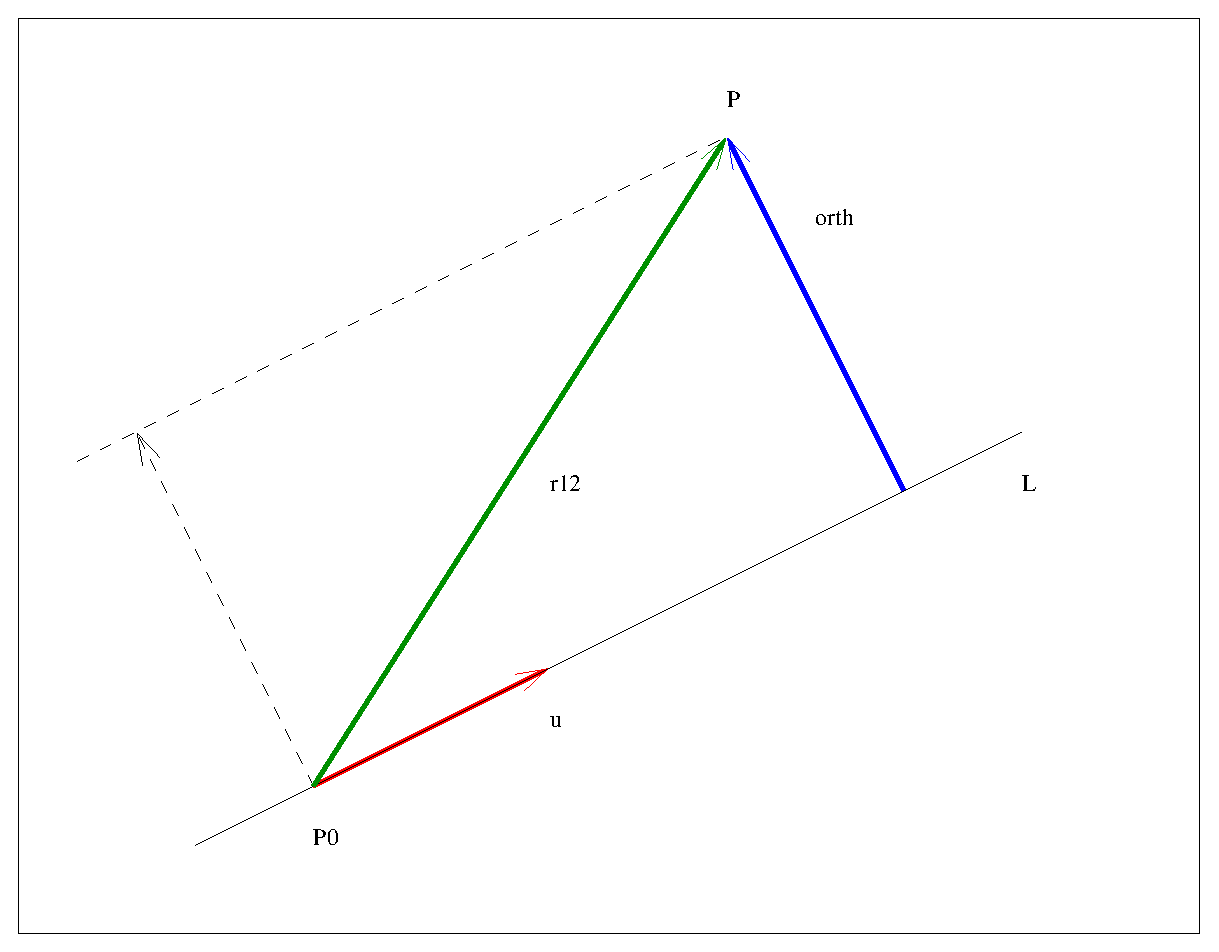
\includegraphics[height=2in]{../../modules/vectors/pictures/ok-distance_point_line.eps}
    \end{figure}
    \end{columns}
\end{frame}
%\begin{frame}
  \frametitle{Distance between point and plane}
  \begin{columns}
  
  \column{0.4\textwidth}
          \psfrag{cP}{$\mathcal{P}$}
          \psfrag{P}{$P(\textbf{r}_1)$}
          \psfrag{P0}{$P_0(\textbf{r}_0)$}
          \psfrag{n}{$\textbf{n}$}
          \psfrag{r12}{$\textbf{r}_1\!-\!\textbf{r}_0$}
          \psfrag{proj}{$\textbf{\text{proj}}_{\bm{n}}(\textbf{r}_1\!-\!\textbf{r}_0)$}
          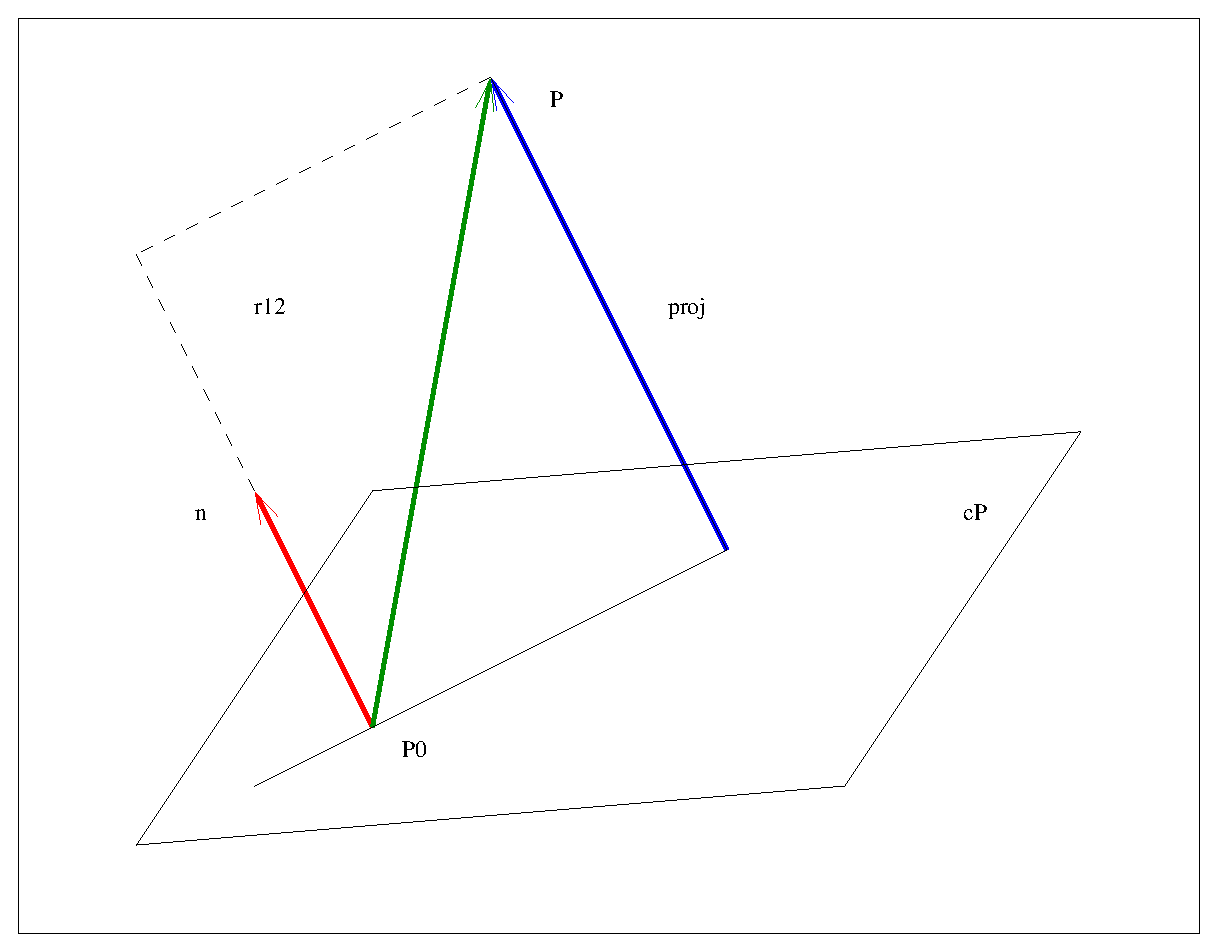
\includegraphics[height=1.3in]{../../modules/vectors/pictures/ok-distance_point_plane.eps}
\column{0.6\textwidth}
\begin{itemize}
\item Given: point $P(\textbf{r}_1)$,
\item plane $\mathcal{P}: \quad (\textbf{r}-\textbf{r}_0)\cdot \textbf{n} = 0$.
\item Goal: find the distance between $P$ and $\mathcal P$. 
\end{itemize}
\alert<1->{Distance} from $P$ to $\mathcal{P}$:
\uncover<2->{
$$d(P,\mathcal{P}) = |\textbf{\text{proj}}_{\bm{n}}(\textbf{r}_1-\textbf{r}_0)|$$
$$d(P,\mathcal{P}) = \frac{|(\textbf{r}_1-\textbf{r}_0) \cdot \textbf{n}|}{|\textbf{n}|}$$}

\uncover<3->{\alert<1->{Scalar equation}:
$P(x_1,y_1,z_1)$
$$\mathcal{P}: ax+by+cz+d=0$$}
\uncover<4->{$$\textbf{n} = \langle a,b,c\rangle$$
$$\boxed{\text{Distance} = \frac{|ax_1+by_1+cz_1+d|}{\sqrt{a^2+b^2+c^2}}}$$}
\end{columns}
\end{frame}
%\begin{frame}
  \frametitle{Parallel lines}
    Lines
    $$L_1: \quad \textbf{r}= \textbf{r}_1+t\textbf{u}_1 \qquad L_2: \quad \textbf{r}= \textbf{r}_2+s\textbf{u}_2$$
\begin{columns}[t]
  \column[T]{6cm}
  \textcolor[rgb]{0.98,0.00,0.00}{Parallel} lines\\
    %\medskip
    \uncover<2->{
    $L_1 || L_2$ $\Longleftrightarrow$
    $\textbf{u}_1$, $\textbf{u}_2$ collinear $\Longleftrightarrow$
    $$\boxed{\textbf{u}_1 \times \textbf{u}_2 = \textbf{0}}$$}
    \uncover<3->{
    \textcolor[rgb]{0.98,0.00,0.00}{Distance}:
    $$d= d(L_1,L_2)  = d(P_1,L_2) = d(P_2,L_1)$$}
    \uncover<4->{
    $$d= d(L_1,L_2) = |\textbf{\text{orth}}_{\bm{u}_1} (\textbf{r}_2-\textbf{r}_1)|$$
    $$\boxed{d = \frac{|(\textbf{r}_2-\textbf{r}_1) \times \textbf{u}_1|}{|\textbf{u}_1|} =\frac{|(\textbf{r}_2-\textbf{r}_1) \times \textbf{u}_2|}{|\textbf{u}_2|}}$$}
    %\textcolor[rgb]{0.98,0.00,0.00}{Identical} lines: $d(L_1,L_2)=0$
    %$$\textbf{u}_1\times \textbf{u}_2 = \textbf{0} \text{ and }
    %(\textbf{r}_2-\textbf{r}_1) \times \textbf{u}_1 = \textbf{0}$$
  \column{6.5cm}
  \begin{figure}
        \psfrag{L1}{$L_1$}
        \psfrag{L2}{$L_2$}
        \psfrag{P1}{$P_1$}
        \psfrag{P2}{$P_2$}
        \psfrag{r21}{$\textbf{r}_2-\textbf{r}_1$}
        \psfrag{u1}{$\textbf{u}_1$}
        \psfrag{u2}{$\textbf{u}_2$}
        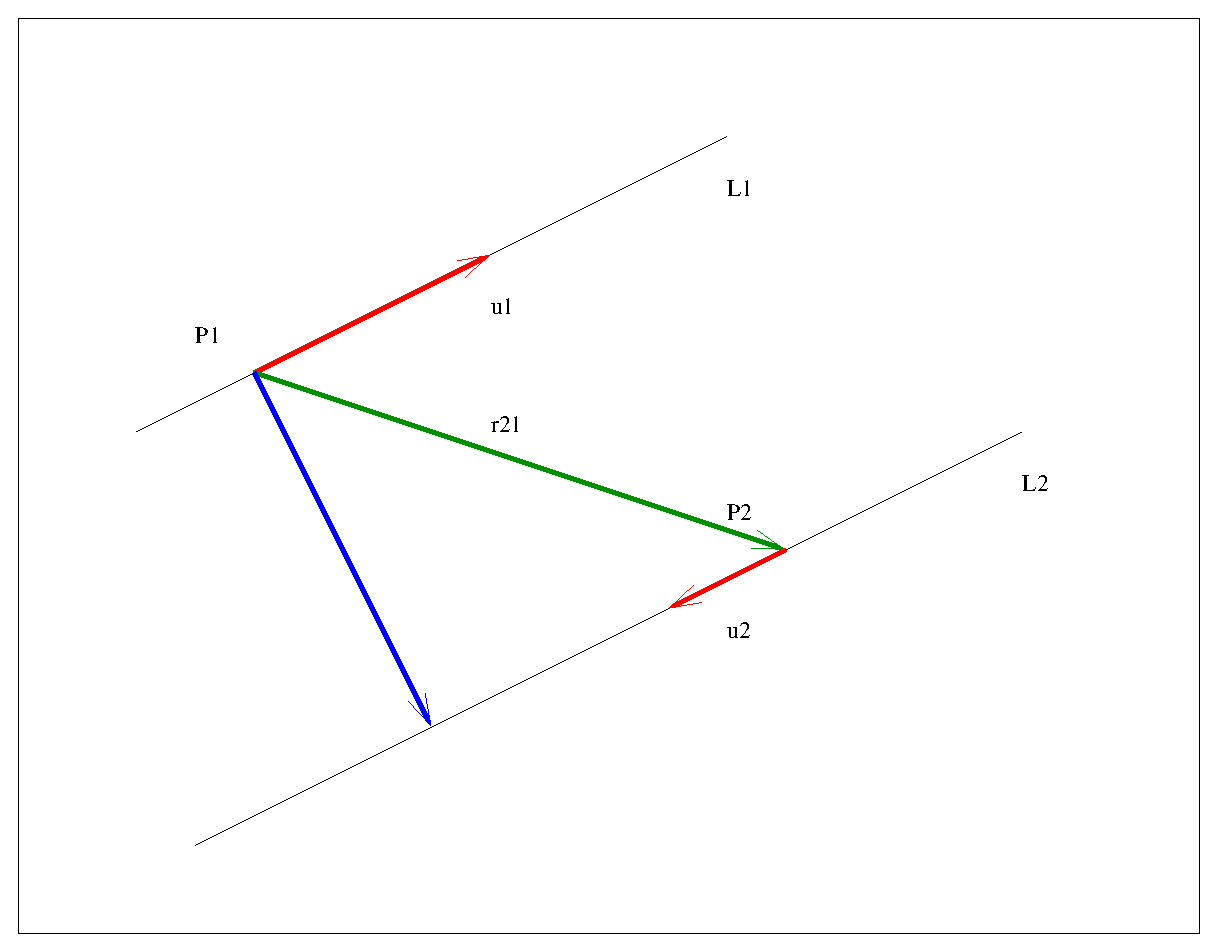
\includegraphics[height=2in]{../../modules/vectors/pictures/ok-distance_parallel_lines.eps}
    \end{figure}
\end{columns}

\end{frame}
%\begin{frame}
\frametitle{Angle between lines}

\begin{columns}
\column{0.4\textwidth}
\begin{pspicture}(-2, -2)(2,2)
\tiny
\renewcommand{\fcScreen}{[-1 0 -0.5] 0}
\fcParallelogramIIId{[1.2 -1.2 1]}{[1.2 1.2 1]}{[-1.2 -1.2 1]}
\fcLineIIId{[-1 -1 -1]}{[1 1 -1]}
\fcLineIIId{[1 -1 1]}{[-1 1 1]} 
%\fcPerpendicularIIId[arrows=->, linecolor=green]{[0 0 -1]}{[1 -1 1] [-1 1 1]}{0.2}
\fcLineIIId[arrows=->, linecolor=blue]{[0 0 -1]}{[0 0 1]}
\fcLineIIId[linestyle=dotted]{[-1 -1 1]}{[1 1 1]}
\fcLineIIId[linecolor=red, arrows=->]{[0 0 -1]}{[0.75 0.75 -1]}
\fcPutIIId[t]{[0.325 0.325 -1.1]}{$\fcv u_1$}
\fcDotIIId{[0 0 -1]}
\fcPutIIId[r]{[-0.1 0.1 -1]}{$P_1$}


\fcDotIIId{[0 0 1]}
\fcPutIIId[r]{[-0.1 0.1 1]}{$P_2$}

\fcLineIIId[linecolor=red, arrows=->]{[0 0 1]}{[-0.75 0.75 1]}
\fcPutIIId[br]{[-0.325 0.325 1]}{$\fcv u_2$}

\fcLineIIId[linecolor=red, arrows=->]{[0 0 1]}{[0.75 0.75 1]}
\fcPutIIId[t]{[0.325 0.325 0.9]}{$\fcv u_1$}
\fcPutIIId[linecolor=brown]{[0 0 1]}{\fcAngleIIId{[0.5 0.5 0]}{[-0.5 0.5 0]}{0.2}}

\fcPutIIId{[2 2 0]}{%
\fcLineIIId[linecolor=red, arrows=->]{[0 0 1]}{[-0.75 0.75 1]}
\fcPutIIId[br]{[-0.325 0.325 1]}{$\fcv u_2$}
\fcLineIIId[linecolor=red, arrows=->]{[0 0 1]}{[0.75 0.75 1]}
\fcPutIIId[t]{[0.325 0.325 0.9]}{$\fcv u_1$}
\fcPutIIId[linecolor=brown]{[0 0 1]}{
\fcAngleIIId{[0.5 0.5 0]}{[-0.5 0.5 0]}{0.3}
\fcPutIIId[l]{[0 0.35 0]}{$\alpha$}
}
}%
\end{pspicture}

\psfrag{L1}{$L_1$}
\psfrag{L2}{$L_2$}
\psfrag{P1}{$P_1$}
\psfrag{P2}{$P_2$}
\psfrag{u1}{$\textbf{u}_1$}
\psfrag{u2}{$\textbf{u}_2$}
\psfrag{a}{$\alpha$}
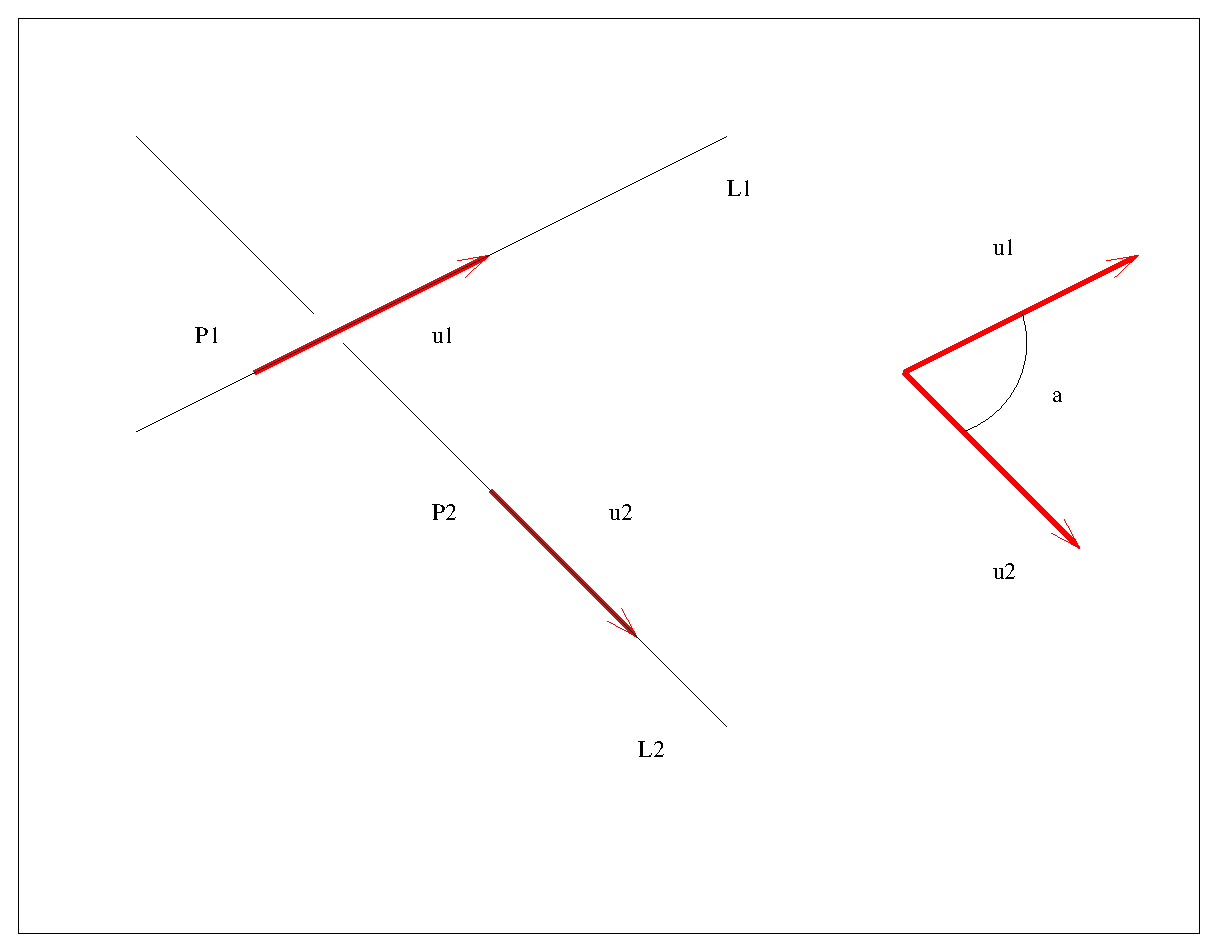
\includegraphics[height=1.4in]{../../modules/vectors/pictures/ok-angle_line_line.eps}
\column{0.6\textwidth}
\begin{itemize}
\item Given: lines $ \begin{array}{rrcl}L_1:&  \textbf{r}&=& \textbf{r}_1+t\textbf{u}_1 \\ L_2:& \textbf{r}&=& \textbf{r}_2+s\textbf{u}_2\end{array}$.
\item Goal: find angle between $L_1$ and $L_2$.
\end{itemize}
\alert<1->{Perpendicular} lines
\uncover<2->{
$L_1 \bot L_2$ $\Longleftrightarrow$
$\textbf{u}_1 \bot \textbf{u}_2$ $\Longleftrightarrow$
$$\boxed{\textbf{u}_1 \cdot \textbf{u}_2 = 0}$$}
\uncover<3->{
\alert<1->{Angle} between lines}
\uncover<4->{
$\alpha$: angle between $L_1$, $L_2$ $\Longleftrightarrow$ 
$\alpha$: acute angle $\textbf{u}_1$, $\textbf{u}_2$}
\uncover<5->{$\Longleftrightarrow$
$$\boxed{\alpha = \arccos\left( \frac{|\textbf{u}_1 \cdot \textbf{u}_2|}{|\textbf{u}_1| \, |\textbf{u}_2|}\right) }$$}
\end{columns}
\end{frame}
%\begin{frame}
\frametitle{Distance between non-parallel lines}
\begin{columns}
\column{0.4\textwidth}
\begin{pspicture}(-2, -2)(2,2)
\tiny
\renewcommand{\fcScreen}{[-1 0 -0.5] 0}
\fcBoundingBox{-2}{-2}{2}{2}
\uncover<2->{%
\fcParallelogramIIId{[1.2 -1.2 1]}{[1.2 1.2 1]}{[-1.2 -1.2 1]}
\fcPutIIId[b]{[-1.2 -1.2 1]}{$\mathcal P$}
}%
\fcLineIIId{[-1 -1 -1]}{[1 1 -1]}
\fcLineIIId{[1 -1 1]}{[-1 1 1]} 
%\fcPerpendicularIIId[arrows=->, linecolor=green]{[0 0 -1]}{[1 -1 1] [-1 1 1]}{0.2}
\fcPutIIId[l]{[-1 1 1]}{$~~L_1$}
\fcPutIIId[r]{[-1 -1 -1.2]}{$L_2$}
\uncover<6->{%
\fcLineIIId[linestyle=dotted]{[0 0 1.3]}{[0 0 -1.3]}%
\fcPutIIId[rt]{[-0.1 0.1 -1]}{$Q_2~~~$}%
}%
\uncover<10->{%
\fcPerpendicularIIId[linestyle=none]{[0 0 -0.125]}{[0 0 1] [1 1 1]}{0.2}%
\fcPerpendicularIIId[linestyle=none]{[0 0 -0.125]}{[0 0 1] [-1 1 1]}{0.2}%
}%
\uncover<13->{%
\fcLineIIId[arrows=->, linecolor=green]{[0.8 -0.8 1]}{[0.9 0.9 -1]}%
\fcLineIIId[arrows=->, linecolor=green]{[0 0 1]}{[0.1 1.7 -1]}%
\fcDotIIId{[0.1 1.7 -1]}%
\fcPutIIId[l]{[0.1 1.7 -1]}{$~~R$}%
\fcPutIIId[l]{[0.05 0.85 0]}{$\fcv r_2- \fcv r_1$}%
}%
\uncover<6->{%
\fcPerpendicularIIId{[0.8 0.8 -1]}{[0 0 -1]}{0.2}
}%
\uncover<14->{\fcLineIIId[arrows=->, linecolor=brown]{[0.8 -0.8 1]}{[0 0 1]}%
\fcLineIIId[arrows=->, linecolor=brown]{[0.9 0.9 -1]}{[0.1 1.7 -1]}%
}%
\uncover<15->{%
\fcPerpendicularIIId{[0.1 1.7 -1]}{[0 0 -1]}{0.2}%
}%
\uncover<11->{%
\fcLineIIId[arrows=->, linecolor=blue]{[0 0 1]}{[0 0 -0.125]}%
\fcPutIIId[r]{[0 0 0.4375]}{$\fcv n~$}
}%
\uncover<4->{%
\fcLineIIId[linestyle=dotted]{[-1 -1 1]}{[1 1 1]}
\fcPutIIId[l]{[1 1 1]}{$~~L_2'$}
}%
\fcLineIIId[linecolor=red, arrows=->]{[0 0 -1]}{[0.75 0.75 -1]}
\fcPutIIId[t]{[0.325 0.325 -1.1]}{$\fcv u_2$}
\fcDotIIId{[0 0 -1]}
\uncover<12->{%
\fcDotIIId{[0.8 -0.8 1]}%
\fcPutIIId[br]{[0.8 -0.8 1]}{$P_1~$}%
\fcDotIIId{[0.9 0.9 -1]}%
\fcPutIIId[tr]{[0.9 0.9 -1]}{$P_2~$}%
}%
\uncover<5->{%
\fcDotIIId{[0 0 1]}
\fcPutIIId[r]{[-0.1 0.1 1]}{$Q_1~~~$}
}%
\fcLineIIId[linecolor=red, arrows=->]{[0 0 1]}{[-0.75 0.75 1]}
\fcPutIIId[br]{[-0.325 0.325 1]}{$\fcv u_1$}
\uncover<2->{
\fcLineIIId[linecolor=red, arrows=->]{[0 0 1]}{[0.75 0.75 1]}
\fcPutIIId[t]{[0.325 0.325 0.9]}{$\fcv u_2$}
}
%\fcPutIIId{[2 2 0]}{%
%\fcLineIIId[linecolor=red, arrows=->]{[0 0 1]}{[-0.75 0.75 1]}
%\fcPutIIId[br]{[-0.325 0.325 1]}{$\fcv u_1$}
%\fcLineIIId[linecolor=red, arrows=->]{[0 0 1]}{[0.75 0.75 1]}
%\fcPutIIId[t]{[0.325 0.325 0.9]}{$\fcv u_2$}
%}%
\end{pspicture}

\column{0.6\textwidth}
\begin{itemize}
\item Given: lines $\begin{array}{rrcl}L_1: & \fcv{r}&=& \fcv{r}_1+t\fcv{u}_1 \\ L_2:& \fcv{r} &=& \fcv{r}_2+s\fcv{u}_2\end{array}$
\item The lines are skew or intersecting, i.e., $\fcv{n} = \fcv{u}_1 \times \fcv{u}_2 \neq \fcv{0}$.
\item Goal: find distance between the lines = $d(L_1, L_2)$ = shortest distance b-n points on the two lines.
\end{itemize}
\end{columns}
\begin{itemize} 
\only<handout:1|1-8>{
\item<2-> Construct plane $\mathcal P$ with directions $\fcv u_1$, $\fcv u_2$ and passing through $L_1$. 
\item<3-> Distance b-n $L_2$ and points on $\mathcal P$ is constant.
\item<4-> Project $L_2$ orthogonally on $\mathcal P$; let the projection be $L_2'$.
\item<5-> Let $L_2' $ and $L_1$ intersect in point $Q_1$.
\item<6-> Let $Q_2$ be the heel of the perpendicular from $Q_1$ onto $Q_2$.
\item<7-> $\Rightarrow$ $Q_1Q_2=d(L_1, L_2)$.
}
\only<handout:1|8-16>{
\item \alert<8,9>{$|Q_1Q_2|=d(L_1, L_2)$}.
}
\only<handout:2|9-16>{
\item<10-> $\fcv Q_1\fcv Q_2 \perp L_1, L_2$ \uncover<11->{$\Rightarrow$  $\fcv Q_1 \fcv Q_2$ is proportional to $\fcv n = \fcv u_1\times \fcv u_2$.}
\item<12-> Pick arbitrary points on $L_1, L_2$ - say, the base points $P_1(\fcv r_1), P_2(\fcv r_2)$.
\item<13-> Let $R$ be such that $\fcv Q_1\fcv R=\fcv P_1 \fcv P_2=\fcv r_2-\fcv r_1$. 
\item<14-> Then $\fcv{P}_2\fcv R$ is proportional to $\fcv u_1$.
\item<15-> $\Rightarrow $ $\fcv Q_2\fcv R= \fcv Q_2  \fcv P_2+\fcv{P}_2\fcv{R}$ is perpendicular to $\fcv n$.
}
\only<handout:3|16->{
\item<16->\alert<16,17>{ $\Rightarrow$ $\fcv Q_1 \fcv Q_2= \fcv {proj} _{\fcv n} (\fcv r_2-\fcv r_1)$.}
}
\only<handout:3|17->{
\item<18-> 
$d(L_1,L_2)  = |\fcv{proj}_{\alert<19>{\fcv{n}}} (\fcv{r}_2-\fcv{r}_1)| \uncover<19->{= \boxed{\frac{|(\fcv{r}_2-\fcv{r}_1)\cdot \alert<19,20>{\fcv{n}} | }{ |\alert<19,20>{\fcv{n}}|}}} \uncover<20->{= \frac{ |(\fcv{r}_2 -\fcv{r}_1 )\cdot (\alert<20>{ \fcv{u}_1\times \fcv{u}_2})|}{ | \alert<20>{\fcv{u}_1\times \fcv{u}_2}|}}$
\item<21-> If lines are intersecting we know $d(L_1,L_2)=0$. \uncover<22->{Since the lines intersect $L_2$ and $L_2'$ coincide.} \uncover<23->{$\Rightarrow$ $(\fcv{r}_2-\fcv{r}_1) \cdot (\fcv{u}_1\times \fcv{u}_2) = 0$} \uncover<24->{$\Rightarrow $ the formula $d(L_1, L_2)= \frac{|(\fcv{r}_2 - \fcv{r}_1 )\cdot (\fcv{u}_1\times \fcv{u}_2)|}{ | \fcv{u}_1\times \fcv{u}_2|}=0$ produces the expected result.}
}
\end{itemize}

\vskip 5cm
\end{frame}


%\begin{frame}
  \frametitle{Parallel line and plane}
     Line $L: \quad \textbf{r}= \textbf{r}_1+t\textbf{u}$\hspace{2cm}
     Plane $\mathcal{P}: \quad (\textbf{r}-\textbf{r}_0) \cdot \textbf{n} = 0$
\bigskip
  \begin{columns}[t]
    \column{6cm}
    Line \textcolor[rgb]{0.98,0.00,0.00}{parallel} to plane\\
    \uncover<2->{
    $L || \mathcal{P}$ $\Longleftrightarrow$
    $\textbf{u} \bot \textbf{n}$ $\Longleftrightarrow$
    $$\boxed{\textbf{u} \cdot \textbf{n} = 0}$$}
    \uncover<3->{
    \textcolor[rgb]{0.98,0.00,0.00}{Distance} from $L$ to $\mathcal{P}$:
    $$d(L,\mathcal{P}) = d(P_1,\mathcal{P})$$}
    \uncover<4->{
    $$d=|\textbf{\text{orth}}_{\bm{u}}(\textbf{r}_1-\textbf{r}_0)| =
    |\textbf{\text{proj}}_{\bm{n}} (\textbf{r}_1-\textbf{r}_0)|$$
    $$d = \frac{|(\textbf{r}_1-\textbf{r}_0) \times \textbf{u}|}{|\textbf{u}|} =
    \textcolor[rgb]{0.98,0.00,0.00}{\frac{|(\textbf{r}_1-\textbf{r}_0)\cdot \textbf{n}|}{|\textbf{n}|}}$$}
    \column{6.5cm}
    \begin{figure}
        \psfrag{L}{$L$}
        \psfrag{cP}{$\mathcal{P}$}
        \psfrag{P1}{$P_1(\textbf{r}_1)$}
        \psfrag{P0}{$P_0(\textbf{r}_0)$}
        \psfrag{u}{$\textbf{u}$}
        \psfrag{n}{$\textbf{n}$}
        \psfrag{r01}{$\textbf{r}_1-\textbf{r}_0$}
        \psfrag{proj}{$\textbf{\text{proj}}_{\bm{n}} (\textbf{r}_1\!-\!\textbf{r}_0)$}
        \psfrag{orth}{$\textbf{\text{orth}}_{\bm{u}}(\textbf{r}_1\!-\!\textbf{r}_0)$}
        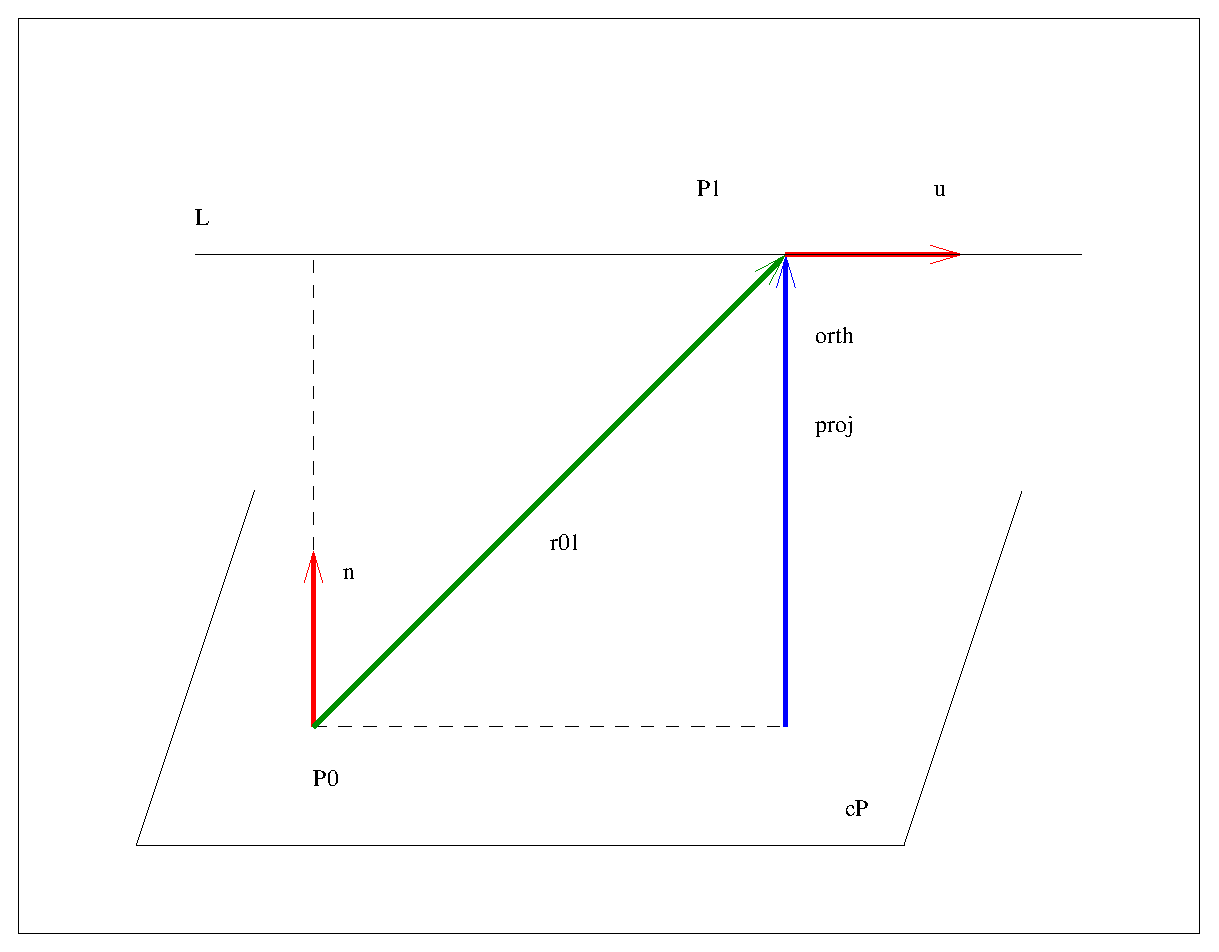
\includegraphics[height=2in]{../../modules/vectors/pictures/ok-parallel_line_plane.eps}
    \end{figure}
    %
  \end{columns}
\end{frame}

%\begin{frame}
\frametitle{Angle between line and plane}
\begin{columns}
\column{0.4\textwidth}
\psset{xunit=2cm, yunit=2cm}
\begin{pspicture}(-1.2, -1.2)(2,2)
\renewcommand{\fcScreen}{[-4 -1 -1] 0}
\tiny 
\fcParallelogramIIId{[-1 -1 0]}{[1 -1 0]}{[-1 1 0]}
\fcPutIIId{[-1 1 0]}{$\mathcal P$}
\fcPerpendicularIIId[linestyle=gray]{[0.5 -0.7 0 ]}{[0 0.5 0] [0 0.5 1]}{0.2}
%\fcDotIIId{[0 0.5 1]}
%\fcPutIIId[b]{[0 0.5 1]}{$P_1(\fcv r_1)$}

\fcLineIIId[arrows=->, linecolor=blue]{[0 0.5 0]}{[0 0.5 1]}
\uncover<5>{%
\fcLineIIId[arrows=->, linewidth=2pt, linecolor=blue]{[0 0.5 0]}{[0 0.5 1]}
}%
\fcPutIIId[l]{[0 0.5 0.5]}{$~\alert<5>{\fcv{proj}_{\fcv n}(\fcv u)}$}

%\fcLineIIId[linecolor=gray]{[0.5 -0.7 0]}{[0.5 -0.7 0.9]}
\fcLineIIId[arrows=->, linecolor=red]{[0.5 -0.7 0]}{[0.5 -0.7 0.5]}
\fcPutIIId[r]{[0.5 -0.7 0.25]}{$\fcv n~~$}

\fcPerpendicularIIId[arrows=<-, linecolor=red]{[0.9 0.9 0.5]}{[0.9 0.9 0] [0.9 0.8 0]}{0.1}
\fcPutIIId[l]{[0.9 0.9 0.25]}{$~~\fcv n$}
\fcDotIIId{[0.9 0.9 0]}
\fcPutIIId[t]{[0.9 0.9 -0.1]}{$P_0(\fcv r_0)$}

\fcPutIIId{[0.5 -0.7 0]}{\fcAngleIIId {[-0.5 1.2 0]} {[-0.5 1.2 1]}{0.2}}
\uncover<4,5>{\fcPutIIId{[0.5 -0.7 0]}{\fcAngleIIId[linewidth=2pt, linecolor=red] {[-0.5 1.2 0]} {[-0.5 1.2 1]}{0.2}}}
\fcPutIIId[l]{[0.4 -0.5 0.1]}{$\alert<4,5>{ \alpha}$}

\fcLineIIId[arrows=->, linecolor=green]{[0.5 -0.7 0]}{[0 0.5 1]}
\uncover<5>{%
\fcLineIIId[arrows=->, linewidth=2pt, linecolor=green]{[0.5 -0.7 0]}{[0 0.5 1]}
}%
\fcPutIIId[tl]{[0.25 -0.1 0.5]}{$ \alert<5>{\fcv u}$}
\fcLineIIId[linestyle=dotted]{[0.56 -0.844 -0.12]}{[0.5 -0.7 0]}
\fcLineIIId{[0.65 -1.06 -0.3]}{[0.56 -0.844 -0.12]}
\fcLineIIId{[0 0.5 1]}{[-0.15 0.86 1.3]}
\fcPutIIId[tl]{[0.65 -1.06 -0.3]}{$~~L$}



\end{pspicture}
\column{0.6\textwidth}
\begin{itemize}
\item Given: line $L: \quad \fcv{r}= \fcv{r}_1+t\fcv{u}$,
\item plane $\mathcal{P}: \quad (\fcv{r}-\fcv{r}_0) \cdot \fcv{n} = 0$.
\item Goal: Find/define angle between line and plane.
\end{itemize}
\end{columns}
Line \alert<1->{perpendicular} to plane
\uncover<2->{
$\Leftrightarrow$
$\fcv{u} \| \fcv{n}$ 
\uncover<3->{%
$\Leftrightarrow$ 
$\boxed{\fcv{u} \times \fcv{n} = \fcv{0}}$
}%
}

\uncover<4->{
\alert<1->{Angle} between line and plane $\alpha$: angle between $L$, $\mathcal{P}$.
$\begin{array}{rcl}
\alert<4,5>{\sin \alpha }&\alert<4,5>{=}& \uncover<5->{\alert<5>{\frac{ \alert<6>{|\fcv{proj}_{\fcv n}\fcv u|}}{|\fcv u|} }}\uncover<6->{ = \frac{ \alert<6>{|\fcv u\cdot\fcv n|} }{ \alert<6>{|\fcv n|} |\fcv u|}}\\
\uncover<7>{ \alpha &=& \arcsin\left(\frac{|\fcv{u} \cdot \fcv{n}|}{|\fcv{u}|  |\fcv{n}|}\right) }
\end{array}
$
}
\end{frame}
%\begin{frame}
  \frametitle{Parallel planes}
\begin{columns}
\column{0.4\textwidth}
\begin{pspicture}(-0.2, -0.2)(2,2)
\tiny
\fcParallelogramIIId{[-1.5 -1.5 -1]}{[-1.5 1.5 -1]}{[1.5 -1.5 -1]}
\fcParallelogramIIId{[-1.5 -1.5 1]}{[-1.5 1.5 1]}{[1.5 -1.5 1]}
\fcPutIIId{[-1.5 -1.5 -1]}{$\mathcal P_1$}
\fcPutIIId{[-1.5 -1.5 1]}{$\mathcal P_2$}
\fcLineIIId{[-1 -1 -1]}{[1 1 -1]}
\fcLineIIId{[-1 -1 1]}{[1 1 1]}
\fcDotIIId{[1 1 1]}
\fcPutIIId[tl]{[1 1 0.9]}{$~~P_2$}
\fcDotIIId{[-1 -1 -1]}
\fcPutIIId[t]{[-1 -1 -1.1]}{$P_1$}
\fcLineIIId[linecolor=gray]{[-1 -1 -1]}{[-1 -1 0.73]}%
\fcLineIIId[linecolor=gray, linestyle=dotted]{[-1 -1 0.73]}{[-1 -1 1]}%
\fcPerpendicularIIId[arrows=<-, linecolor=red]{[-1 -1 0.1]}{[-1 -1 -1] [0 0 -1]}{0.2}%
\fcPutIIId[r]{[-1 -1 -0.45]}{$\fcv n_1~~$}

\fcPerpendicularIIId[linecolor=gray]{[1 1 0.73]}{[1 1 -1] [-1 -1 -1]}{0.2}%
\fcLineIIId[linecolor=gray, linestyle=dotted]{[1 1 0.73]}{[1 1 1]}%

\fcPerpendicularIIId[arrows=<-, linecolor=red]{[1 1 1.7]}{[1 1 1] [0 0 1]}{0.2}%
\fcPutIIId[l]{[1 1 1.35]}{$~~\fcv n_2$}

\fcLineIIId[linecolor=blue]{[-1 -1 -1]}{[0.53 0.53 0.53]}
\fcLineIIId[arrows=->, linecolor=blue, linestyle=dotted]{[0.53 0.53 0.53]}{[1 1 1]}
\fcPutIIId[l]{[0 0 0]}{$~~~\fcv r_2- \fcv r_1$}
\end{pspicture}
\column{0.6\textwidth}
\begin{itemize}
\item Given: planes $\begin{array}{rrcl}
\mathcal{P}_1:& (\textbf{r} - \alert<7>{\textbf{r}_1})\alert<7>{ \cdot \alert<6>{\textbf{n}_1}} &=& 0 \\
\mathcal{P}_2:& (\textbf{r} - \alert<7>{\textbf{r}_2}) \alert<7>{\cdot \alert<6>{\textbf{n}_2}} &=& 0
\end{array}.
$
\item Goal: Establish whether planes are parallel, find distance b-n planes.
\end{itemize}
\end{columns}
Planes are \alert<1->{parallel} \uncover<2->{$\mathcal{P}_1 || \mathcal{P}_2$ $\Leftrightarrow$ $\textbf{n}_1$, $\textbf{n}_2$ collinear $\Leftrightarrow$
$\boxed{\textbf{n}_1 \times \textbf{n}_2 = \textbf{0}}$. }

\uncover<3->{\alert<1->{Distance}:\quad
$d(\mathcal{P}_1,\mathcal{P}_2) = |\textbf{\text{proj}}_{\textbf{n}_1} (\textbf{r}_2-\textbf{r}_1)| \uncover<4->{=\boxed{\frac{|(\textbf{r}_2-\textbf{r}_1)\cdot \textbf{n}_1|}{|\textbf{n}_1|}}}$
} %uncover3

\uncover<5->{%
\noindent Assume $\alert<6>{ \fcv n_1=\fcv n_2=( a,b,c) }$
\uncover<6->{$\Rightarrow$ plane eq-ns:
$\begin{array}{r@{~}r@{~}c@{~}l}
\mathcal{P}_1 :& \alert<6>{a}x+\alert<6>{b}y+\alert<6>{c}z &=& \alert<7>{d_1}\\
\mathcal{P}_2 :& \alert<6>{a}x+\alert<6>{b}y+\alert<6>{c}z &=& \alert<7>{d_2}
\end{array}.$
}
\uncover<7->{
\[
\Rightarrow \boxed{d(\mathcal{P}_1,\mathcal{P}_2) = \frac{|\alert<7>{d_2-d_1}|}{\sqrt{a^2+b^2+c^2}}}
\]
}
}%uncover5
\end{frame}

%\begin{frame}
\frametitle{Angle between planes}
\begin{columns}
\column{0.35\textwidth}
\centering
\psset{xunit=1.2cm, yunit=1.2cm}
\begin{pspicture}(-2, -2.5)(2,1.4)
\tiny
\renewcommand{\fcScreenStyle}{x}
%\fcAxesIIId{2}{2}{2}
\fcParallelogramIIId[linecolor=green!30]{[1 0 -1]}{[1 1 -1]}{[0 0 0]}
\fcParallelogramIIId[linecolor=magenta!30]{[1 0 0]}{[1 1 0]}{[-1 0 0]}
\fcParallelogramIIId[linecolor=green!30]{[0 0 0]}{[-1 0 1]}{[0 1 0]}
\uncover<6->{
\fcParallelogramIIId[linecolor=cyan!30]{[1 0 -1]}{[1 0 1]}{[-1 0 -1]}
}
\fcParallelogramIIId[linecolor=green!30]{[1 -1 -1]}{[1 0 -1]}{[0 -1 0]}
\fcParallelogramIIId[linecolor=magenta!30]{[1 -1 0]}{[1 0 0]}{[-1 -1 0]}
\fcParallelogramIIId[linecolor=green!30]{[0 0 0]}{[0 -1 0]}{[-1 0 1]}

\uncover<6->{%
\fcPutIIId[b]{[0.8 0 1.1]}{$\mathcal P_3$}
\fcPolyLineIIId{[1 0 -1] [1 0 1] [-1 0 1]}
\fcLineIIId[linestyle=dashed]{[-1 0 1]}{[-1 0 -0.5]}
\fcPolyLineIIId{[-1 0 -0.5] [-1 0 -1] [-0.5 0 -1]}
\fcLineIIId[linestyle=dashed]{[-0.5 0 -1]}{[1 0 -1]}
}
\fcPolyLineIIId[linestyle=dashed]{[-1 -0.35 0] [-1 1 0] [0 1 0]}
\fcPolyLineIIId{[-1 -0.35 0] [-1 -1 0] [1 -1 0] [1 1 0] [0 1 0]}
\fcPolyLineIIId{[0 1 0] [-1 1 1] [-1 -1 1] [1 -1 -1] [1 1 -1] [0.33 1 -0.33]}%
\fcLineIIId[linestyle=dashed]{[0.33 1 -0.33]}{[0 1 0]}%
%\uncover<9->{%
%\fcPerpendicularIIId[arrows=<-, linecolor=red]{[1.7 0 0.3]}{[1 0 -1]}{0.2}%
%\fcDotIIId{[0.7 0 -0.7]}%
%\fcPutIIId[tl]{[0.7 0 -0.7]}{$~~P_1$}%
%\fcPutIIId[l]{[1.5 0 0]}{$~\fcv n_1$}
%}%
%\fcPerpendicularIIId[arrows=<-, linecolor=red]{[1 0 1]}{[-1 0 1]}{0.2}
\uncover<9->{%
\fcLineIIId[arrows=<-, linecolor=red]{[1 0 1]}{[0 0 0]}
\fcPutIIId[tl]{[0.85 0 0.85]}{$~~~~\fcv n_1$}%
}%
%\uncover<9->{%
%\fcPerpendicularIIId[arrows=<-, linecolor=red]{[0.8 0.8 0.8]}{[0.8 0.8 0] [0.6 0.8 0]}{0.2}%
%\fcDotIIId{[0.8 0.8 0]}
%\fcPutIIId[bl]{[0.8 0.8 0]}{$~~P_2$}
%\fcPutIIId[bl]{[0.8 0.8 0.5]}{$~~\fcv n_2$}
%}%

\fcLineIIId[linecolor=gray]{[0 -1 0]}{[0 1 0]}
\fcPutIIId[b]{[0 -1 0.1]}{$L$}
%\fcPerpendicularIIId[arrows=<-, linecolor=red]{[0 0 0.8]}{[-1 0 0]}{0.1}
\uncover<9->{%
\fcLineIIId[arrows=<-, linecolor=red]{[0 0 0.8]}{[0 0 0]}
\fcPutIIId[bl]{[0 0 0.5]}{$~~\fcv n_2$}
}%
\fcPolyLineIIId{[-0.5 0 0.5] [0 0 0]}%
\fcLineIIId[linestyle=dashed]{[0 0 0]}{[0.2 0 -0.2]}%
\uncover<3-4>{%
\fcPerpendicularIIId{[-0.5 0 0.5]}{[0 1 0]}{0.2}%
}%
\uncover<3->{%
\fcDotIIId{[-0.5 0 0.5]}%
\fcPutIIId[b]{[-0.5 0 0.6]}{$Q_1$}
}%

\fcLineIIId[linestyle=dashed]{[0 0 0]}{[-0.7 0 0]}%
\fcLineIIId{[0 0 0]}{[0.7 0 0]}%
\uncover<4->{%
\fcDotIIId{[-0.7 0 0]}%
\fcPutIIId[t]{[-0.7 0 -0.1]}{$Q_2$}
}%
\uncover<4>{%
\fcPerpendicularIIId[linestyle=dashed]{[-0.7 0 0]}{[0 1 0]}{0.2}%
}%
\uncover<5->{%
\fcAngleIIId[linecolor=blue]{[-1 0 1]}{[-1 0 0]}{0.3}%
\fcPutIIId[rb]{[-0.3 0 0.1]}{$\alpha$}%
}%
\uncover<11->{\fcAngleIIId[linecolor=blue]{[0 0 1]}{[1 0 1]}{0.3}}%
\uncover<13->{%
\fcLineIIId[arrows=->, linecolor=blue]{[0 0 0]}{[0 -0.8 0]}%
\fcPutIIId[l]{[0 -0.5 0]}{$~\fcv u$}%
}%
\fcPutIIId[tr]{[-1 -1 0]}{$\mathcal P_2$}
\fcPutIIId[tr]{[-1 -1 1]}{$\mathcal P_1$}
%\fcParallelogramHollowIIId{[-1 -1 0]}{[1 -1 0]}{[-1 1 0]}
%\fcParallelogramHollowIIId{[1 -1 -1]}{[1 1 -1]}{[-1 -1 1]}
\end{pspicture}
\uncover<6->{%
\psset{xunit=1cm, yunit=1cm}
\begin{pspicture}(-1.2, -1.2)(1.2, 1.4)
\tiny
\renewcommand{\fcScreen}{[0 1 0] 0}
\fcBoundingBox{-1.5}{-1.5}{1.5}{1.5}
\fcParallelogramIIId[linecolor=cyan!30]{[1 0 -1]}{[1 0 1]}{[-1 0 -1]}
\fcPutIIId[t]{[0 0 -0.1]}{$O$}
\fcPutIIId[b]{[0.8 0 1.1]}{$\mathcal P_3$}
\uncover<9->{%
\fcPutIIId[bl]{[0 0 0.6]}{$~~\fcv n_2$}
\fcPutIIId[tl]{[0.85 0 0.85]}{$~~\fcv n_1$}%
}%uncover9
\uncover<9>{%
\fcLineIIId[arrows=<-, linecolor=red]{[0 0 0.8]}{[0 0 0]}%
\fcLineIIId[arrows=<-, linecolor=red]{[1 0 1]}{[0 0 0]}%
}%uncover9
\uncover<10->{%
\fcPerpendicularIIId[arrows=<-, linecolor=red]{[0 0 0.8]}{[1 0 0]}{0.12}%
\fcPerpendicularIIId[arrows=<-, linecolor=red]{[1 0 1]}{[1 0 -1]}{0.2}%
}%
\fcLineIIId{[0 0 0]}{[-0.7 0 0]}%
\fcPolyLineIIId{[-0.5 0 0.5] [0 0 0]}%
\fcAngleIIId[linecolor=blue]{[-1 0 1]}{[-1 0 0]}{0.35}%
\fcPutIIId[rb]{[-0.3 0 0.15]}{$\alpha$}%
\uncover<11->{%
\fcAngleIIId[linecolor=blue]{[0 0 1]}{[1 0 1]}{0.35}%
\fcPutIIId[lb]{[0.1 0 0.35]}{$\alpha~~$}%
}%
\fcDotIIId{[-0.5 0 0.5]}%
\fcPutIIId[b]{[-0.5 0 0.6]}{$Q_1$}
\fcDotIIId{[-0.7 0 0]}%
\fcPutIIId[t]{[-0.7 0 -0.1]}{$Q_2$}
\end{pspicture}
}%
\vskip 6cm
\column{0.65\textwidth}
\begin{itemize}
\item Given: planes 
$\begin{array}{rrcl}
\mathcal{P}_1:&  (\fcv{r} - \fcv{r}_1) \cdot \alert<9>{\fcv{n}_1 }&=& 0 \\
\mathcal{P}_2:& (\fcv{r} - \fcv{r}_2) \cdot \alert<9>{\fcv{n}_2} &=& 0
\end{array}
$
\item Goal: \alert<4>{define} and find the angle between the two planes.
\only<handout:1| 1-6>{%
\item<2-> Let $L$ - intersection line of two planes.
\item<3-> In $\mathcal P_1$, drop perpendicular from arbitrary point $Q_1$ to $L$.
\item<4-> In $\mathcal P_2$, raise a perpendicular from the perpendicular heel.
\item<5-> \alert<4>{Define angle $\alpha$} b-n $\mathcal P_1, \mathcal P_2$ = acute angle b-n two perpendiculars.
}%
\item<6-> \alert<6,7>{Consider the plane $\mathcal P_3$ spanned by the two constructed perpendiculars.}

\only<handout:1| 1-6>{%
\vskip 0.57cm
}%
\only<handout: 2| 7->{%
\item<8-> $\mathcal P_3$ is orthogonal to $L$.
\item<9-> $\Rightarrow$ $\mathcal P_3$ contains the normal vectors $\fcv n_1$, $\fcv n_2$.
\item<10-> $\fcv n_1\perp \fcv O\fcv Q_{1}$ and $\fcv n_2\perp \fcv O\fcv Q_{2}$.
\item<11-> 
$
\begin{array}{rcl}
\alpha &=& \text{acute} \angle (\fcv{n}_1,\fcv{n}_2) \\
\alpha &=&\arccos{\left( \frac{|\fcv{n}_1 \cdot \fcv{n}_2|}{|\fcv{n}_1|\, |\fcv{n}_2|}\right)}
\end{array}
$
\item<12-> $\perp$ planes: $\Rightarrow$ $\alpha = \frac{\pi}{2} \Longleftrightarrow \boxed{\fcv{n}_1 \cdot \fcv{n}_2 = 0}$.
\item<13-> Direction of $L$ is $\fcv{u} = \fcv{n}_1 \times \fcv{n}_2$.
}%onlyr<7->
\end{itemize}

\vfill

\end{columns}
\vskip 5cm

\end{frame}




%\begin{frame}
\frametitle{Line from Point and Direction}
\begin{columns}
\column{0.3\textwidth}
\psset{xunit=1cm, yunit=1cm}
\begin{pspicture}(-0.2,-0.2)(3.5,2)
\tiny
\fcFullDot{0}{0}
\rput[tl](0,-0.1){$O$}
\psline(0, 1.7)(3.5,0.3)
\fcFullDot{0.5}{1.5}
\rput[bl](0.5, 1.5){$P_0$}
\uncover<4->{
\psline[arrows=->, linecolor=red](0.5,1.5)(2.5,0.7)
}
\psline[arrows=->, linecolor=blue](1,1.3)(2, 0.9)
\rput[b](1.5,1.2) {$\fcv u$}
\rput[l](3.5,0.3){$L$}

\uncover<2->{\psline[arrows=->](0,0)(0.5,1.5)
\rput[l](0.25, 0.75){$~~\fcv r_0$}
}
\uncover<3->{%
\psline[arrows=->](0,0)(2.5, 0.7)
\rput[b](2.5, 0.75){$P$}
\rput[t](1.25, 0.2){$\fcv r$}
}
\end{pspicture}

\column{0.7\textwidth}
\begin{itemize}
\item Suppose we have line $L$ that passes through point $P_0$ and has non-zero direction $\textbf{u}$.
\item<2-> Denote by $\fcv r_0=\fcv{OP}_0$ the position vector of $P_0$.
\item<3->$P$ with position vector $\textbf{r}$ is on $L$ $\Leftrightarrow$ 
\item<4->$\textbf{P}_0\textbf{P}$ has the same direction as $\textbf{u}$ $\Leftrightarrow$
\item<5-> $\textbf{P}_0\textbf{P}$ is a scalar multiple of $\textbf{u}$ $\Leftrightarrow$
\item<6-> $\textbf{r}-\textbf{r}_0 = t\textbf{u}$  for some real number $t$.
\end{itemize}
\end{columns}
\uncover<7->{
\begin{definition}
The equation 
\[
\fcv{r} = \fcv{r}_0+t\fcv{u}
\]
is called a parametric vectorial equation of the the line $L$.
\end{definition}
}
\end{frame}

\begin{frame}
\frametitle{Line from Point and Direction}
\begin{columns}
  \column{6cm}
\begin{itemize}
 \item Point $P_0(x_0,y_0,z_0)$, $\textbf{r}_0=\langle x_0,y_0,z_0\rangle$;
\item Direction $\textbf{u}=\langle u_1,u_2,u_3\rangle$.
\end{itemize}
  \column{5cm}
 $L$: line with direction $\textbf{u}$, \\passing through $P_0$
\end{columns}

\begin{columns}
  \column{6cm}
    \uncover<2->{$P$ with position vector $\textbf{r}$ is on $L$ $\leftrightarrow$ \\ }
    \uncover<3->{\medskip $\textbf{r} = \textbf{r}_0+t\textbf{u}$ $\leftrightarrow$\\}
    \uncover<4->{\medskip $\langle x,y,z\rangle = \langle x_0,y_0,z_0\rangle + t\langle u_1,u_2,u_3\rangle$ $\leftrightarrow$\\}
    \uncover<5->{\medskip \textcolor[rgb]{0.98,0.00,0.00}{Parametric scalar equations}:\\
    $\boxed{\left\{ \begin{array}{ll}
           x & = x_0 + t u_1 \\
	   y & = y_0 + t u_2 \\
           z & = z_0 + t u_3
          \end{array}
\right.}$  \\ for some real parameter $t$ }

  \column{6.5cm}
    \begin{figure}
        \psfrag{O}{$O$}
        \psfrag{x}{$x$}
        \psfrag{y}{$y$}
        \psfrag{z}{$z$}
        \psfrag{L}{$L$}
        \psfrag{P}{$P(x,y,z)$}
        \psfrag{P0}{$P_0(x_0,y_0,z_0)$}
        \psfrag{r}{$\textbf{r}$}
        \psfrag{u}{$\textbf{u}=\langle u_1,u_2,u_3\rangle$}
        \psfrag{r0}{$\textbf{r}_0$}
        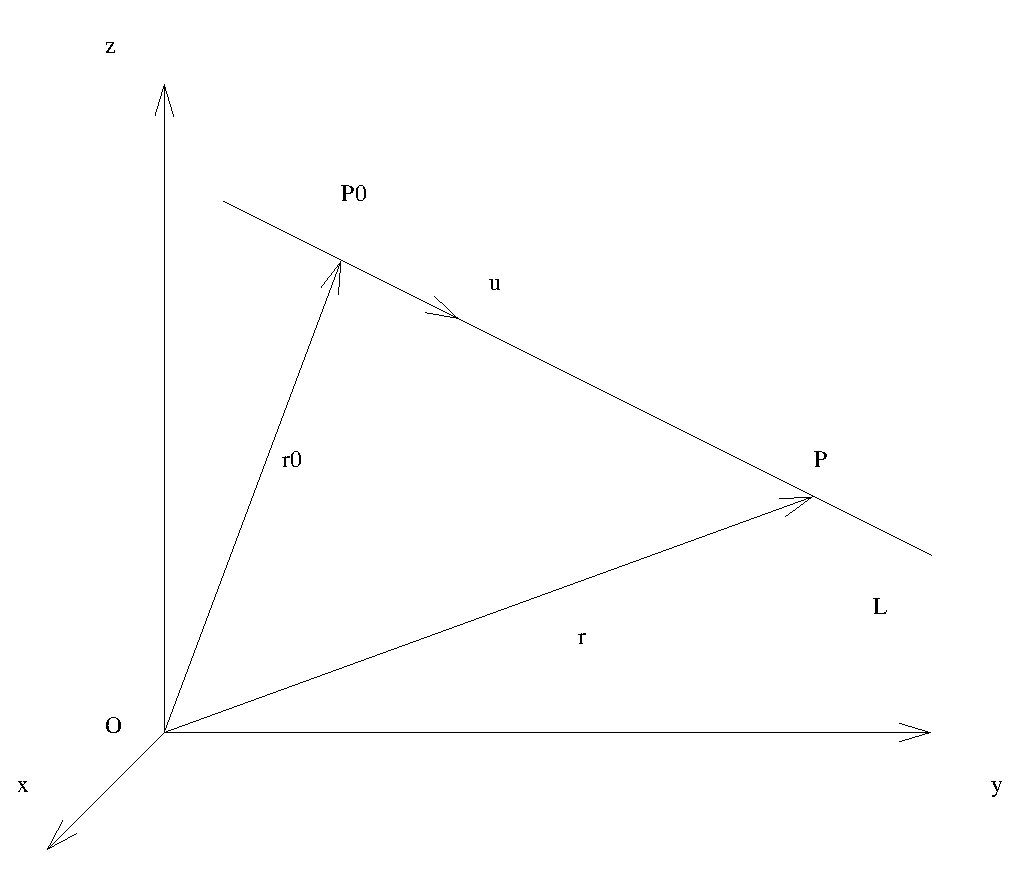
\includegraphics[height=2in]{../../modules/vectors/pictures/ok-line_point_direction_scalar.eps}
    \end{figure}
\end{columns}
\end{frame}

\begin{frame}
\uncover<1->{ $$\left\{ \begin{array}{ll}
           x & = x_0 + t u_1 \\
	   y & = y_0 + t u_2 \\
           z & = z_0 + t u_3
          \end{array}
\right. \Longrightarrow \boxed{\frac{x-x_0}{u_1} = \frac{y-y_0}{u_2} = \frac{z-z_0}{u_3}} \text{ \textcolor[rgb]{0.98,0.00,0.00}{Symmetric equations}}$$}

\uncover<2->{Caution! If $u_2=0$ (for example), then:
%
$$\frac{x-x_0}{u_1} = \frac{z-z_0}{u_3} \quad  \text{ and } \quad y=y_0 $$}

\uncover<3->{Example: Line with direction $\textbf{u} = \langle 4,5,6\rangle$ through $P_0(1,2,3)$:}
\begin{itemize}
 \item<4-> Parametric vectorial equation:
%
$$\textbf{r} = \langle 1,2,3\rangle + t \langle 4,5,6\rangle \leftrightarrow
\textbf{r} = \langle 1+4t, 2+5t, 3+6t\rangle$$
%
\item<5-> Parametric scalar equations:
%
$$\left\{ \begin{array}{ll}
           x & = 1 + 4t \\
	   y & = 2+5t \\
           z & = 3+6t
          \end{array}
\right. , \quad t \text{ real number.}$$
%
\item<6-> Symmetric equations:
%
$$\frac{x-1}{4} = \frac{y-2}{5} = \frac{z-3}{6}\; .$$
\end{itemize}

\end{frame}
%\begin{frame}
\frametitle{Torque}
\begin{columns}
\begin{pspicture}(-0.2, -1.2)(2, 1.2)
\tiny%
\fcBoundingBox{-0.2}{-1.2}{2}{1.2}%
\uncover<1-2>{\fcLineIIId{[0 0 -0.2]}{[0 0 -1]}}%
\uncover<3->{\fcLineIIId[arrows=->]{[0 0 -0.2]}{[0 0 -1]}}%
\uncover<3->{\fcLineIIId[arrows=->]{[0 0 1]}{[0 0 0.1]}}
%\fcAxesIIId{1}{1}{1}
\fcPolyLineIIId{[0.2  0 0.1] [0.1 0.173205 0.1] [-0.1 0.173205 0.1] [-0.2 0 0.1] [-0.1 -0.173205 0.1] [0.1 -0.173205 0.1] [0.2 0 0.1]}%
\fcPolyLineIIId{[-0.1 -0.173205 -0.1] [0.1 -0.173205 -0.1] [0.2 0 -0.1] [0.1 0.173205 -0.1]}%
\fcLineIIId{[-0.1 -0.173205 -0.1]}{[-0.1 -0.173205 0.1]}%
\fcLineIIId{[0.1 -0.173205 -0.1]}{ [0.1 -0.173205 0.1]}%
\fcLineIIId{[0.2 0 -0.1]} {[0.2 0 0.1]}%
\fcLineIIId{[0.1 0.173205 -0.1]}{[0.1 0.173205 0.1]}%
\uncover<2->{\fcPolyLineIIId[linecolor=blue]{[0.15 -0.259808 0] [0.3 0 0] [0.15 0.259808 0]  [0.04 0.259808 0] }%
\fcLineIIId[linecolor=blue]{[0.15 0.259808 0]} {[0.15 0.259808 0] 5 \fcVectorTimesScalar}%
}%
\uncover<4->{\fcLineIIId[linecolor=blue, arrows=->]{[0.15 0.259808 0]} {[0.15 0.259808 0] 5 \fcVectorTimesScalar}%
\fcPutIIId[b]{[0.32 0.65 0.1]}{$\fcv r$}%
}%
\uncover<3->{\fcAngleIIId[arrows=->, linecolor=blue]{[0.15 0.259808 0] }{ [0.4 0.2 0]}{1.2}}%
\uncover<4->{\fcLineIIId[arrows=->, linecolor=red]{[0.75 1.29904 0]}{[1 0.5 1]}}
\uncover<9->{\fcPutIIId[r]{[0 0 -0.5]}{$\tau~$}}
\end{pspicture}

\column{0.7\textwidth}
\begin{itemize}
\item If we tighten a bolt \uncover<2->{using a wrench,} \uncover<3->{it moves in direction perpendicular to the motion of the wrench.}
\item<4-> Let arm of the wrench: given by vector $\fcv r$. 
\end{itemize}
\end{columns}
\begin{itemize}
\item<4-> Suppose we are applying a force $\fcv F$ at arm of the wrench. The force has three components: 
\begin{itemize}
\item<5-> component $\fcv F_o$ orthogonal to the plane of rotation
\item<6-> component $\fcv F_\rho$ in the plane of rotation towards/away from the center
\item<7-> component $\fcv F_\theta$ tangent to the motion of the wrench.
\end{itemize}
\item<8-> Only $\fcv F_\theta$ contributes to the bolt motion.
\item<9-> The force of bolt motion $\fcv \tau$ is proportional to length of wrench.
\item<10-> It turns out $\fcv \tau = \fcv r \times (\fcv F_\rho+\fcv F_\theta)$, where \alert<10>{$\times$ is the vector cross product}.
\end{itemize}
\end{frame}

%\begin{frame}
\begin{itemize}
\item To each permutation $\sigma$, assign $ n$ pairs of numbers $(1,\sigma(1))$, $(2, \sigma(2))$,\dots $(n,\sigma (n))$.
\item<2-> Consider a $n\times n$ chess board. \uncover<3->{Interpret pair $(k,\sigma(k))$ as $(row,column)$-coordinates in the board.} 
\item<4-> For each pair $(k,\sigma( k))$, place a rook on the board.
\item \uncover<5->{ Example: 
$
\begin{array}{rcl}
\alert<5,6>{\sigma(1)}  &\alert<5,6>{=}  & \alert<5,6>{2} \\
\alert<7,8>{\sigma(2)}  &\alert<7,8>{=}  & \alert<7,8>{3} \\
\alert<9,10>{\sigma(3)} &\alert<9,10>{=} & \alert<9,10>{4}\\
\alert<11,12>{\sigma(4)}&\alert<11,12>{=}& \alert<11,12>{1}
\end{array}
$, pairs:
$\begin{array}{rcl}
\alert<5,6>{(1,\sigma(1))}  &\alert<5,6>{=}  &\alert<5,6>{(1,2)} \\ 
\alert<7,8>{(2,\sigma(2))}  &\alert<7,8>{=}  &\alert<7,8>{(2,3)} \\ 
\alert<9,10>{(3,\sigma(3))} &\alert<9,10>{=} &\alert<9,10>{(3,4)} \\ 
\alert<11,12>{(4,\sigma(4))}&\alert<11,12>{=}&\alert<11,12>{(4,1)}
\end{array}
. $ 

Corresponding peaceful rook placement:
}

\uncover<2->{
\psset{xunit=2cm, yunit=2cm}
\begin{pspicture}(-0.2,0)(1,1.2)
\tiny
\fcBoundingBox{-0.2}{-0.1}{1}{1.2}
\psgrid[gridlabels=0, subgriddiv=4](0,0)(0,0)(1,1)
\uncover<3->{
\rput(-0.125, 0.875){$1$}
\rput(-0.125, 0.625){$2$}
\rput(-0.125, 0.375){$3$}
\rput(-0.125, 0.125){$4$}
\rput(0.125, 1.125){$1$}
\rput(0.375, 1.125){$2$}
\rput(0.625, 1.125){$3$}
\rput(0.875, 1.125){$4$}
}
\uncover<13>{
\psline[arrows=<->, linecolor=red](0,0.875)(1,0.875)
\psline[arrows=<-, linecolor=red](0.375,0)(0.375,0.875)
\psline[arrows=<->, linecolor=red](0,0.625)(1,0.625)
\psline[arrows=<->, linecolor=red](0.625,0)(0.625,1)
\psline[arrows=<-, linecolor=red](0,0.375)(0.875,0.375)
\psline[arrows=<->, linecolor=red](0.875,0)(0.875,1)
\psline[arrows=->, linecolor=red](0.125,0.125)(1,0.125)
\psline[arrows=->, linecolor=red](0.125,0.125)(0.125,1)
}
\uncover<5>{
\rput(0.125, 0.875){\alert<5>{\textbf{?}}}
\rput(0.375, 0.875){\alert<5>{\textbf{?}}}
\rput(0.625, 0.875){\alert<5>{\textbf{?}}}
\rput(0.875, 0.875){\alert<5>{\textbf{?}}}
}
\uncover<7>{
\rput(0.125, 0.625){\alert<7>{\textbf{?}}}
\rput(0.375, 0.625){\alert<7>{\textbf{?}}}
\rput(0.625, 0.625){\alert<7>{\textbf{?}}}
\rput(0.875, 0.625){\alert<7>{\textbf{?}}}
}
\uncover<9>{
\rput(0.125, 0.375){\alert<9>{\textbf{?}}}
\rput(0.375, 0.375){\alert<9>{\textbf{?}}}
\rput(0.625, 0.375){\alert<9>{\textbf{?}}}
\rput(0.875, 0.375){\alert<9>{\textbf{?}}}
}
\uncover<11>{
\rput(0.125, 0.125){\alert<11>{\textbf{?}}}
\rput(0.375, 0.125){\alert<11>{\textbf{?}}}
\rput(0.625, 0.125){\alert<11>{\textbf{?}}}
\rput(0.875, 0.125){\alert<11>{\textbf{?}}}
}
\uncover<6->{\fcFullDot{0.375}{0.875}}
\uncover<8->{\fcFullDot{0.625}{0.625}}
\uncover<10->{\fcFullDot{0.875}{0.375}}
\uncover<12->{\fcFullDot{0.125}{0.125}}
\end{pspicture}
}
\item<13-> $\sigma(k)$ are different $\Rightarrow$ rook placements are peaceful: rooks never hit one another. I.e., no two points lie on same column or row.
\end{itemize}

\vskip 10cm
\end{frame}

%\begin{frame}
\frametitle{$\fcv{orth}_{\fcv u}$ is a linear operator}
\begin{theorem}
$\alert<14>{ \alert<13>{ \fcv{orth}_{\fcv u}(\alert<12>{ \fcv v_1 +\fcv v_2}) }= \alert<10>{ \fcv{orth}_{\fcv u} \fcv v_1 } +\alert<11>{\fcv{orth}_{\fcv u} \fcv v_2}}$
\end{theorem}
\begin{proof}
\begin{columns}
\column{0.3\textwidth}
Geometric proof:
\uncover<8->{
\psset{xunit=0.9cm, yunit=0.9cm}
\begin{pspicture}(-0.5,-0.7)(3.8,4.2)%
\tiny%
\fcBoundingBox{-0.5}{-0.7}{3.8}{4.2}%
\uncover<9->{%
\fcParallelogramIIId{[0 -0.5 -0.5]}{[0 3 0]}{[0 0 3]}%
\fcPutIIId[lt]{[0.3 3 3]}{$\mathcal P$}%
}%
\fcLineIIId[arrows=->]{[0 0 0]}{[1 0 0]}%
\fcPutIIId[t]{[0.5 0 -0.1]}{$\fcv u$}%
\uncover<10->{%
\fcPerpendicularIIId{[1 1 2]}{[0 1 2]}{0.2}%
}%
\fcLineIIId[arrows=->]{[0 0 0]}{[1 1 2]}%
\fcPutIIId[tl]{[0.5 0.5 1]}{$\fcv v_1$}%
\uncover<10->{%
\fcLineIIId[linecolor=blue, arrows=->]{[0 0 0]}{[0 1 2]}%
\fcPutIIId[rb]{[0 0.5 1]}{$\color{blue}{\alert<14>{ \fcv{orth}_{\fcv u } \fcv v_1}}$}%
}%
\uncover<11->{\fcPerpendicularIIId{[1 2 0]}{[0 2 0]}{0.2}}%
\fcLineIIId[arrows=->]{[0 0 0]}{[1 2 0]}%
\fcPutIIId[t]{[0.5 1 -0.1]}{$\fcv v_2$}%
\uncover<11->{\fcLineIIId[linecolor=blue, arrows=->]{[0 0 0]}{[0 2 0]}}%
\uncover<11->{%
\fcLineIIId[arrows=->]{[1 1 2]}{[2 3 2]}%
\fcPutIIId[b]{[1.5 2 2]}{$\fcv v_2$}%
}%
\uncover<11->{%
\fcPerpendicularIIId{[2 3 2]}{[0 3 2]}{0.2}%
}%
\uncover<11->{%
\fcLineIIId[arrows=->, linecolor=blue]{[0 1 2]}{[0 3 2]}%
\fcPutIIId[b]{[0 2 2.2]}{$\color{blue}{\alert<14>{ \fcv{orth}_{\fcv u} \fcv v_2} }$}%
}%
\uncover<13->{%
\fcLineIIId[arrows=->, linecolor=blue]{[0 0 0]}{[0 3 2]}%
\fcPutIIId[l]{[0 2 1.3]}{$\color{blue}{\alert<14>{ \fcv{orth}_{\fcv u} (\fcv v_1 +\fcv v_2)}}$}%
}%
\uncover<12->{%
\fcLineIIId[arrows=->]{[0 0 0]}{[2 3 2]}%
\fcPutIIId[lt]{[1 1.5 1]}{$\fcv v_1 +\fcv v_2$}%
}%
\uncover<14>{%
\fcLineIIId[linewidth=1.5pt, arrows=->, linecolor=red]{[0 0 0]}{[0 3 2]}%
\fcLineIIId[linewidth=1.5pt, arrows=->, linecolor=red]{[0 1 2]}{[0 3 2]}%
\fcLineIIId[linewidth=1.5pt, arrows=->, linecolor=red]{[0 0 0]}{[0 1 2]}%
}%
\end{pspicture}
\uncover<9->{\alert<9>{Let $\mathcal P$: plane $\perp \fcv u$.}}
} %uncover
\column{0.7\textwidth}
Algebraic proof:

\small
\noindent \uncover<2->{
$
\begin{array}{r@{~}c@{~}l}
\fcv{orth}_{\fcv u}(\fcv v_1+\fcv v_2)&=& (\fcv v_1+\fcv v_2)- \alert<3>{\fcv{proj}_{\fcv u}(\fcv v_1 +\fcv v_2)}\\
\uncover<3->{&=&(\alert<4>{\fcv v_1}+\alert<5>{\fcv v_2})\alert<4,5>{-} \left(\alert<3>{ \alert<4>{\fcv{proj}_{\fcv u}(\fcv v_1)} +\alert<5>{\fcv{proj}_{\fcv u}(\fcv v_2)}}\right)} \\
\uncover<4->{&=&\left(\alert<4,6>{\fcv v_1- \fcv{proj}_{\fcv u}(\fcv v_1)}\right)+\left(\alert<5,7>{\fcv v_2-\fcv{proj}_{\fcv u}(\fcv v_2)}\right)}\\
\uncover<6->{&=& \alert<6>{\fcv{orth}_{\fcv u} \fcv v_1}+\alert<7>{\fcv{orth}_{\fcv u} \fcv v_2}}
\end{array}
$
}
\normalsize
\end{columns}
\end{proof}
\end{frame}
%\begin{frame}
\frametitle{Justification of Linearity of $\times$ Product}
\begin{theorem}
$\alertNoH{11}{\fcv u\times (\fcv v_1+\fcv v_2)=\fcv u \times\fcv v_1 +\fcv u\times \fcv v_2 }$.
\end{theorem}
\begin{proof}[Geometric justification]
\begin{columns}
\column{0.41\textwidth}
\uncover<2->{%
\psset{xunit=1cm, yunit=1cm}
\begin{pspicture}(-1.5, -0.8)(3.6,4.15)
\tiny%
\fcBoundingBox{-1.5}{-0.8}{3.6}{4.15}%
\fcParallelogramIIId{[0 -1.5 -0.45]}{[0 -2.1 3.1]}{[0 3.7 0]}%
\fcPutIIId[lt]{[0.3 3 3]}{$\mathcal P$}%
\fcLineIIId[arrows=->]{[0 0 0]}{[1 0 0]}%
\fcPutIIId[t]{[0.5 0 -0.1]}{$\fcv u$}%
\uncover<1-4>{%
\fcPerpendicularIIId{[1 1 2]}{[0 1 2]}{0.2}%
\fcLineIIId[arrows=->]{[0 0 0]}{[1 1 2]}%
\fcPutIIId[tl]{[0.5 0.5 1]}{$\fcv v_1$}%
\fcPerpendicularIIId{[1 2 0]}{[0 2 0]}{0.2}%
\fcLineIIId[arrows=->]{[0 0 0]}{[1 2 0]}%
\fcPutIIId[t]{[0.5 1 -0.1]}{$\fcv v_2$}%
\fcLineIIId[linecolor=blue, arrows=->]{[0 0 0]}{[0 2 0]}%
\fcLineIIId[arrows=->]{[1 1 2]}{[2 3 2]}%
\fcPutIIId[b]{[1.5 2 2]}{$\fcv v_2$}%
\fcPerpendicularIIId{[2 3 2]}{[0 3 2]}{0.2}%
\fcLineIIId[linecolor=blue, arrows=->]{[0 0 0]}{[0 1 2]}%
\fcPutIIId[rb]{[0 0.5 1]}{$\color{blue}{ \fcv{orth}_{\fcv u } \fcv v_1}$}%
\fcLineIIId[arrows=->, linecolor=blue]{[0 1 2]}{[0 3 2]}%
\fcPutIIId[b]{[0 2 2.2]}{$\color{blue}{\fcv{orth}_{\fcv u} \fcv v_2 }$}%
\fcLineIIId[arrows=->, linecolor=blue]{[0 0 0]}{[0 3 2]}%
\fcPutIIId[l]{[0 2 1.3]}{$\color{blue}{ \fcv{orth}_{\fcv u} (\fcv v_1 +\fcv v_2)}$}%
\fcLineIIId[arrows=->]{[0 0 0]}{[2 3 2]}%
\fcPutIIId[lt]{[1 1.5 1]}{$\fcv v_1 +\fcv v_2$}%
}%uncover
\uncover<4>{%
\fcLineIIId[linewidth=1.5pt, arrows=->, linecolor=red]{[0 0 0]}{[0 1 2]}%
\fcLineIIId[linewidth=1.5pt, arrows=->, linecolor=red]{[0 1 2]}{[0 3 2]}%
\fcLineIIId[linewidth=1.5pt, arrows=->, linecolor=red]{[0 0 0]}{[0 3 2]}%
}%
\uncover<5->{%
\fcLineIIId[arrows=->]{[0 0 0]}{[0 1 2]}%
\fcLineIIId[arrows=->]{[0 1 2]}{[0 3 2]}%
\fcLineIIId[arrows=->]{[0 0 0]}{[0 3 2]}%
\fcLineIIId[arrows=->]{[0 0 0]}{[0 2 0]}%
\fcPerpendicularIIId{[1 0 0]}{[0 -1 -2]}{0.2}%
\fcPerpendicularIIId{[1 0 0]}{[0 -2 0]}{0.2}%
\fcPutIIId[rb]{[0 0.5 1]}{$\alertNoH{5}{\fcv v_1}$}%
\fcPutIIId[l]{[0 2 1.3]}{$\alertNoH{5}{\fcv v_1 +\fcv v_2}$}%
\fcPutIIId[b]{[0 2 2.2]}{$\alertNoH{5}{\fcv v_2 }$}%
\fcPutIIId[b]{[0 1 0]}{$\alertNoH{5}{\fcv v_2 }$}%
}%
\uncover<8->{\fcLineIIId[arrows=->, linecolor=blue]{[0 0 0]}{[0 -2 1]}}%
\uncover<9->{\fcLineIIId[arrows=->, linecolor=blue]{[0 0 0]}{[0 0 2]}}%
\uncover<10->{%
\fcLineIIId[arrows=->, linecolor=blue]{[0 0 0]}{[0 -2 3]}%
\fcAngleIIId[linecolor=magenta, arrows=->]{[0 3 2]}{[0 -2 3]}{0.6}%
}%
\uncover<8->{\fcAngleIIId[linecolor=orange, arrows=->]{[0 0.5 1]}{[0 -2 1]}{0.4}}%
\uncover<9->{\fcAngleIIId[linecolor=brown, arrows=->]{[0 2 0]}{[0 0 2]}{0.5}}%
\uncover<11->{%
\fcLineIIId[linewidth=1.5pt, arrows=->, linecolor=red]{[0 0 0]}{[0 -2 1]}%
\fcLineIIId[linewidth=1.5pt, arrows=->, linecolor=red]{[0 0 0]}{[0 0 2]}%
\fcLineIIId[linewidth=1.5pt, arrows=->, linecolor=red]{[0 0 0]}{[0 -2 3]}%
\fcLineIIId[linewidth=1.5pt, arrows=->, linecolor=red]{[0 0 2]}{[0 -2 3]}%
}%
\uncover<10->{\fcPutIIId[l]{[0 -1.8 2.7]}{${\fcv u \times (\fcv v_1 +\fcv v_2)}$}}%
\uncover<9->{\fcPutIIId[r]{[0 0 1]}{${\fcv u \times \fcv v_2}$}}%
\uncover<8->{\fcPutIIId[tr]{[0 -0.5 0.25]}{${\fcv u \times \fcv v_1}$}}%
\end{pspicture}
}%uncover
\column{0.59\textwidth}
\small
\uncover<2->{
$\begin{array}{r@{~}c@{~}l}
\alertNoH{4}{\fcv u\times \fcv v_1} &=& \alertNoH{4}{\fcv u\times \fcv{orth}_{\fcv u}\fcv v_1} \\
\alertNoH{4}{\fcv u\times \fcv v_2} &=&\alertNoH{4}{ \fcv u\times \fcv{orth}_{\fcv u}\fcv v_2}\\
\alertNoH{4}{\fcv u\times (\fcv v_1+\fcv v_2)} &=&  \fcv u\times \left(\alertNoH{3}{ \fcv{orth}_{\fcv u} \left(\fcv v_1+\fcv v_2\right)} \right)\\
\uncover<3->{ &=& \alertNoH{4}{ \fcv u\times \left( \alertNoH{3}{ \fcv{orth}_{\fcv u} \left(\fcv v_1\right)+\fcv{orth}_{\fcv u} \left(\fcv v_2\right)} \right)}}
\end{array}
$
\uncover<4->{\alertNoH{5}{$\Rightarrow$ suffices to prove theorem when  $\fcv v_1, \fcv v_2\perp \fcv u $}.}
\uncover<6->{Since $(a\fcv u)\times \fcv v= a(\fcv u \times \fcv v)$ $\Rightarrow$ suffices to prove theorem when $|\fcv u|=1$. }

\uncover<7->{When $|\fcv u| =1$, applying $\fcv u\times $ rotates all vectors in the plane $\mathcal P$ at angle $\frac{\pi}{2}$.
}
}%uncover
\uncover<11->{The statement of the theorem now follows from the fact that rotation preserves sums of vectors.
}
\end{columns}
\end{proof}
\end{frame}


%\begin{frame}
\begin{example}
$L$ - line with direction $\textbf{u} = ( 4,5,6)$ passing through $P_0(1,2,3)$. Find
\begin{itemize}
\item a parametric vectorial equation of $L$;
\item a parametric scalar equation of $L$;
\item symmetric equations of $L$.
\end{itemize}


\uncover<2->{%
Parametric vectorial equation:

$
\alert<2>{\fcv{r} =}\uncover<3->{\alert<3>{( 1,2,3) + t ( 4,5,6) \leftrightarrow \fcv{r} = ( 1+4t, 2+5t, 3+6t)}}
$
} %uncover

\uncover<3->{
Parametric scalar equations:

$
\left|
\begin{array}{rl}
\alert<4>{x =}& \uncover<5->{\alert<4>{ 1 + 4t}} \\
\alert<4>{y =}& \uncover<5->{\alert<4>{2+5t}} \\
\alert<4>{z =}& \uncover<5->{\alert<4>{3+6t}}
\end{array}
\right. , \quad t \text{ real number.}
$
} %uncover

\uncover<6->{ \alert<6>{Symmetric equations:}
\uncover<7->{

$
\displaystyle
\frac{x-1}{4} = \frac{y-2}{5} = \frac{z-3}{6}\; .
$
}
}
\end{example}
\end{frame}


%\begin{frame}
\frametitle{Permutations and permutation signs}
\begin{itemize}
\item Let $\sigma: \{1,2,\dots n\}\to \{1,2,\dots, n\}$ be one to one function.
\item<2-> Since $\sigma $ - one to one, $\left(\sigma(1), \sigma(2), \dots, \sigma(n) \right)$ have no repetition.
\uncover<3->{
\begin{definition}
A one-to-one function from the set $\{1,2,\dots, n\}$ to itself is called a \alert<4>{permutation} (``shuffling'').
\end{definition}
}
\item<4-> There are $n!$ different permutations: 
\begin{itemize}
\item<5-> there are $n$ ways to select $\sigma(1)$,
\item<6-> $n-1$ ways to select $\sigma(2)$ (one number is already taken),
\item<7-> and so on,  total: $n \cdot (n-1)\cdots 1 =n!$ ways to make a permutation.
\end{itemize}
\end{itemize}
\end{frame}
%\begin{frame}
\frametitle{Sign of permutation}
\begin{itemize}
\item Given two sequences of numbers, define them to be transpositions of one another if one is obtained from the other with a \alertNoH{1}{single swap of \alertNoH{5}{neighboring} numbers}.
\item<2-> \alertNoH{2}{$(2,\alertNoH{3}{3,4},1) $ and $(2,\alertNoH{3}{4,3},1) $ are} \uncover<3->{ \alertNoH{3}{transpositions} of one another.}

\alertNoH{4}{$(2,3,4,1) $ and $(1,3,4,2) $ are} \uncover<5->{\alertNoH{5}{\textbf{not} transpositions} of one another.}
\item<6-> Write the numbers $\left(\sigma(1),\sigma(2), \dots, \sigma(n)\right)$ in a sequence.
\item<7-> Using transpositions, get from $\left(\sigma(1),\sigma(2), \dots, \sigma(n)\right)$ to the properly ordered sequence $1,2,\dots, n$.
\item<8-> Number of transpositions used varies depending how we do it, but parity (even-ness) of \# of transpositions is always the same.
\item<10-> If $sign(\sigma)=1$,  $\sigma$ is called even, if $sign(\sigma)=-1$, $\sigma$ is called odd.
\end{itemize}
\uncover<9->{
\begin{definition}
If we can get from $\left(\sigma(1),\sigma(2), \dots, \sigma(n)\right)$ to $(1,2,\dots, n)$ with even \# of transpositions, define $sign(\sigma)$ to be $1$, else define $sign(\sigma)$ to be $-1$.
\end{definition}
}
\end{frame}

%\begin{frame}
\begin{itemize}
\item To each permutation $\sigma$, assign $ n$ pairs of numbers $(1,\sigma(1))$, $(2, \sigma(2))$,\dots $(n,\sigma (n))$.
\item<2-> Consider a $n\times n$ chess board. \uncover<3->{Interpret pair $(k,\sigma(k))$ as $(row,column)$-coordinates in the board.} 
\item<4-> For each pair $(k,\sigma( k))$, place a rook on the board.
\item \uncover<5->{ Example: 
$
\begin{array}{rcl}
\alert<5,6>{\sigma(1)}  &\alert<5,6>{=}  & \alert<5,6>{2} \\
\alert<7,8>{\sigma(2)}  &\alert<7,8>{=}  & \alert<7,8>{3} \\
\alert<9,10>{\sigma(3)} &\alert<9,10>{=} & \alert<9,10>{4}\\
\alert<11,12>{\sigma(4)}&\alert<11,12>{=}& \alert<11,12>{1}
\end{array}
$, pairs:
$\begin{array}{rcl}
\alert<5,6>{(1,\sigma(1))}  &\alert<5,6>{=}  &\alert<5,6>{(1,2)} \\ 
\alert<7,8>{(2,\sigma(2))}  &\alert<7,8>{=}  &\alert<7,8>{(2,3)} \\ 
\alert<9,10>{(3,\sigma(3))} &\alert<9,10>{=} &\alert<9,10>{(3,4)} \\ 
\alert<11,12>{(4,\sigma(4))}&\alert<11,12>{=}&\alert<11,12>{(4,1)}
\end{array}
. $ 

Corresponding peaceful rook placement:
}

\uncover<2->{
\psset{xunit=2cm, yunit=2cm}
\begin{pspicture}(-0.2,0)(1,1.2)
\tiny
\fcBoundingBox{-0.2}{-0.1}{1}{1.2}
\psgrid[gridlabels=0, subgriddiv=4](0,0)(0,0)(1,1)
\uncover<3->{
\rput(-0.125, 0.875){$1$}
\rput(-0.125, 0.625){$2$}
\rput(-0.125, 0.375){$3$}
\rput(-0.125, 0.125){$4$}
\rput(0.125, 1.125){$1$}
\rput(0.375, 1.125){$2$}
\rput(0.625, 1.125){$3$}
\rput(0.875, 1.125){$4$}
}
\uncover<13>{
\psline[arrows=<->, linecolor=red](0,0.875)(1,0.875)
\psline[arrows=<-, linecolor=red](0.375,0)(0.375,0.875)
\psline[arrows=<->, linecolor=red](0,0.625)(1,0.625)
\psline[arrows=<->, linecolor=red](0.625,0)(0.625,1)
\psline[arrows=<-, linecolor=red](0,0.375)(0.875,0.375)
\psline[arrows=<->, linecolor=red](0.875,0)(0.875,1)
\psline[arrows=->, linecolor=red](0.125,0.125)(1,0.125)
\psline[arrows=->, linecolor=red](0.125,0.125)(0.125,1)
}
\uncover<5>{
\rput(0.125, 0.875){\alert<5>{\textbf{?}}}
\rput(0.375, 0.875){\alert<5>{\textbf{?}}}
\rput(0.625, 0.875){\alert<5>{\textbf{?}}}
\rput(0.875, 0.875){\alert<5>{\textbf{?}}}
}
\uncover<7>{
\rput(0.125, 0.625){\alert<7>{\textbf{?}}}
\rput(0.375, 0.625){\alert<7>{\textbf{?}}}
\rput(0.625, 0.625){\alert<7>{\textbf{?}}}
\rput(0.875, 0.625){\alert<7>{\textbf{?}}}
}
\uncover<9>{
\rput(0.125, 0.375){\alert<9>{\textbf{?}}}
\rput(0.375, 0.375){\alert<9>{\textbf{?}}}
\rput(0.625, 0.375){\alert<9>{\textbf{?}}}
\rput(0.875, 0.375){\alert<9>{\textbf{?}}}
}
\uncover<11>{
\rput(0.125, 0.125){\alert<11>{\textbf{?}}}
\rput(0.375, 0.125){\alert<11>{\textbf{?}}}
\rput(0.625, 0.125){\alert<11>{\textbf{?}}}
\rput(0.875, 0.125){\alert<11>{\textbf{?}}}
}
\uncover<6->{\fcFullDot{0.375}{0.875}}
\uncover<8->{\fcFullDot{0.625}{0.625}}
\uncover<10->{\fcFullDot{0.875}{0.375}}
\uncover<12->{\fcFullDot{0.125}{0.125}}
\end{pspicture}
}
\item<13-> $\sigma(k)$ are different $\Rightarrow$ rook placements are peaceful: rooks never hit one another. I.e., no two points lie on same column or row.
\end{itemize}

\vskip 10cm
\end{frame}

%\begin{frame}
\frametitle{Square matrices}
\begin{itemize}
\item Let $A$ be $n\times n$ (square) table of numbers.
\item<2-> Technical term: $A$ is a (square) \emph{matrix}.
\item<3-> Matrices are often denoted by surrounding with $\left(\right)$-parenthesis:
\[
A=\left(
\begin{array}{ccccc}
a_{\alertNoH{7}{1}\alertNoH{10}{1}} & a_{\alertNoH{7}{1}\alertNoH{11}{2}} & a_{\alertNoH{7}{1}3}& \dots & a_{\alertNoH{7}{1}\alertNoH{12}{n}}\\
a_{\alertNoH{8}{2}\alertNoH{10}{1}} & a_{\alertNoH{8}{2}\alertNoH{11}{2}} & a_{\alertNoH{8}{2}3}& \dots & a_{\alertNoH{8}{2}\alertNoH{12}{n}}\\
\vdots \\
a_{\alertNoH{9}{n}\alertNoH{10}{1}} & a_{\alertNoH{9}{n}\alertNoH{11}{2}} & a_{\alertNoH{9}{n}3}& \dots & a_{\alertNoH{9}{n}\alertNoH{12}{n}}
\end{array}
\right).
\]
\vphantom{ $n^{th}$ Second First row}
\only<7>{\alertNoH{7}{First row}}
\only<8>{\alertNoH{8}{Second row}}
\only<9>{\alertNoH{9}{$n^{th}$ row}}
\only<10>{\alertNoH{10}{First column}}
\only<11>{\alertNoH{11}{Second column}}
\only<12>{\alertNoH{12}{$n^{th}$ column}}

\item<4-> Most common convention for matrix notation:
\begin{itemize}
\item $(i,j)^{th}$ entry of a matrix = denoted by letter with indices $i,j$, such as $a_{ij}$
\item<5-> no comma between indices $i,j$ in $a_{ij}$
\item<6-> first index stands for row, second - for column.
\end{itemize}
\item<13-> Non-square matrices: used \& important but we discuss them elsewhere.
\end{itemize}
\end{frame}



\begin{frame}

\begin{itemize}
\item The determinant $\det A$ of a square matrix $A$ is a number written as:
\[
\det A= \left|\begin{array}{ccccc}
a_{11} & a_{12} & a_{13}& \dots & a_{1n}\\
a_{21} & a_{22} & a_{23}& \dots & a_{2n}\\
\vdots \\
a_{n1} & a_{n2} & a_{n3}& \dots & a_{nn}
\end{array} \right|
\]
\item<2-> The formula for the determinant is:

\[\det A=\sum_{\text{all permutations }\alertNoH{3}{\sigma}} a_{\alertNoH{4}{1\alertNoH{3}{\sigma}(1)}} a_{\alertNoH{4}{2\alertNoH{3}{\sigma}(2)}} \dots a_{\alertNoH{4}{n\alertNoH{3}{\sigma}(n)}} \alertNoH{6}{ sign(\alertNoH{3}{\sigma})} \quad .
\]
\item<3-> For every permutation $\sigma$ we have one summand.
\item<4-> Every pair $(k,\sigma(k))$ can be identified with a peaceful of a rook placement (as described in previous slides/lectures).
\item<5-> For each rook placement we have a summand obtained by multiplying the numbers on which the rooks are standing.
\item<6-> The sign of each summand is determined by the sign of the permutation.
\end{itemize}

\vskip 10cm
\end{frame}

%\begin{frame}

\frametitle{$2\times 2$ determinants}
\[
\det \left|
\begin{array}{cc}
\only<2,4>{\alert<2,4>{\bullet}}\only<1,3,5->{ a_{11}} & \only<1,2,4,6->{a_{12}}\only<3,5>{\alert<3,5>{\bullet}} \\
\only<1,2,4,6->{ a_{21}}\only<3,5>{\alert<3,5>{\bullet}} & \only<1,3,5->{ a_{22}}\only<2,4>{\alert<2,4>{\bullet}}
\end{array}
\right| = \uncover<4->{\alert<4>{ a_{11} a_{22}}} \uncover<6>{\alert<6>{-}}\uncover<5->{ \alert<5>{a_{12}a_{21}}}
\]
\begin{itemize}
\item We specialize the $n\times n$ determinant formula to the case $n=2$.
\item<2-> There are two peaceful rook placements for a $2\times 2$ chessboard.
\item<4-> For each peaceful rook placement we got one summand.
\item<6-> The permutation $(\sigma(1), \sigma(2))=(2,1)$ is odd, so one of the summands comes with negative sign.
\end{itemize}\end{frame}
%\begin{frame}

\frametitle{$3\times 3$ determinants}
\[
\det \left|
\begin{array}{ccc}
\only<1-2,4-6,8->{ a_{11}}\only<handout:0|3,7>{\alertNoH{3,7}{\bullet}} & \only<1-3,5-7,9->{a_{12}}\only<handout:0|4,8>{\alertNoH{4,8}{\bullet}} &\only<1-4,7->{a_{13}}\only<handout:0|5,6>{\alertNoH{5,6}{\bullet}}\\
\only<1-4,6,7,9->{ a_{21}}\only<handout:0|5,8>{\alertNoH{5,8}{\bullet}} & \only<1-2,4-5,7->{ a_{22}}\only<handout:0|3,6>{\alertNoH{3,6}{\bullet}} & \only<1-3,5,6,8->{a_{23}}\only<handout:0|4,7>{\alertNoH{4,7}{\bullet}}\\
\only<1-3,5,7->{ a_{31}}\only<handout:0|4,6>{\alertNoH{4,6}{\bullet}} & \only<1-4,6,8->{ a_{32}}\only<handout:0|5,7>{\alertNoH{5,7}{\bullet}} & \only<1-2,4-7,9->{a_{33}}\only<handout:0|3,8>{\alertNoH{3,8}{\bullet}}
\end{array}
\right| =\begin{array}{l} \uncover<3->{\alertNoH{3}{a_{11}a_{22}a_{33}}} \uncover<4->{\alertNoH{4}{+}}
\uncover<4->{\alertNoH{4}{a_{12}a_{23}a_{31}}} \\
\uncover<5->{\alertNoH{5}{+}} \uncover<5->{\alertNoH{5}{a_{13}a_{21}a_{32}}}\\
\uncover<6->{\alertNoH{6}{-}} \uncover<6->{\alertNoH{6}{a_{13}a_{22}a_{31}}} \uncover<7->{\alertNoH{7}{-}} \uncover<7->{\alertNoH{7}{a_{11}a_{23}a_{32}}} \\
\uncover<8->{\alertNoH{8}{-}} \uncover<8->{\alertNoH{8}{a_{12}a_{21}a_{33}}}
\end{array}
\]
\begin{itemize}
\item We specialize the $n\times n$ determinant formula to the case $n=3$.
\item<2-> There are $6=3!$ peaceful rook placements for a $3\times 3$ chessboard.
\item<3-> For each peaceful rook placement we got one summand.
\item<9-> The rook placements along the down-right ``broken'' diagonals correspond to even permutations, and the rook placements along the right-up ``broken'' diagonals correspond to negative permutations.
\end{itemize}\end{frame}

%\begin{frame}
\frametitle{Justification of Linearity of $\times$ Product}
\begin{theorem}
$\alertNoH{11}{\fcv u\times (\fcv v_1+\fcv v_2)=\fcv u \times\fcv v_1 +\fcv u\times \fcv v_2 }$.
\end{theorem}
\begin{proof}[Geometric justification]
\begin{columns}
\column{0.41\textwidth}
\uncover<2->{%
\psset{xunit=1cm, yunit=1cm}
\begin{pspicture}(-1.5, -0.8)(3.6,4.15)
\tiny%
\fcBoundingBox{-1.5}{-0.8}{3.6}{4.15}%
\fcParallelogramIIId{[0 -1.5 -0.45]}{[0 -2.1 3.1]}{[0 3.7 0]}%
\fcPutIIId[lt]{[0.3 3 3]}{$\mathcal P$}%
\fcLineIIId[arrows=->]{[0 0 0]}{[1 0 0]}%
\fcPutIIId[t]{[0.5 0 -0.1]}{$\fcv u$}%
\uncover<1-4>{%
\fcPerpendicularIIId{[1 1 2]}{[0 1 2]}{0.2}%
\fcLineIIId[arrows=->]{[0 0 0]}{[1 1 2]}%
\fcPutIIId[tl]{[0.5 0.5 1]}{$\fcv v_1$}%
\fcPerpendicularIIId{[1 2 0]}{[0 2 0]}{0.2}%
\fcLineIIId[arrows=->]{[0 0 0]}{[1 2 0]}%
\fcPutIIId[t]{[0.5 1 -0.1]}{$\fcv v_2$}%
\fcLineIIId[linecolor=blue, arrows=->]{[0 0 0]}{[0 2 0]}%
\fcLineIIId[arrows=->]{[1 1 2]}{[2 3 2]}%
\fcPutIIId[b]{[1.5 2 2]}{$\fcv v_2$}%
\fcPerpendicularIIId{[2 3 2]}{[0 3 2]}{0.2}%
\fcLineIIId[linecolor=blue, arrows=->]{[0 0 0]}{[0 1 2]}%
\fcPutIIId[rb]{[0 0.5 1]}{$\color{blue}{ \fcv{orth}_{\fcv u } \fcv v_1}$}%
\fcLineIIId[arrows=->, linecolor=blue]{[0 1 2]}{[0 3 2]}%
\fcPutIIId[b]{[0 2 2.2]}{$\color{blue}{\fcv{orth}_{\fcv u} \fcv v_2 }$}%
\fcLineIIId[arrows=->, linecolor=blue]{[0 0 0]}{[0 3 2]}%
\fcPutIIId[l]{[0 2 1.3]}{$\color{blue}{ \fcv{orth}_{\fcv u} (\fcv v_1 +\fcv v_2)}$}%
\fcLineIIId[arrows=->]{[0 0 0]}{[2 3 2]}%
\fcPutIIId[lt]{[1 1.5 1]}{$\fcv v_1 +\fcv v_2$}%
}%uncover
\uncover<4>{%
\fcLineIIId[linewidth=1.5pt, arrows=->, linecolor=red]{[0 0 0]}{[0 1 2]}%
\fcLineIIId[linewidth=1.5pt, arrows=->, linecolor=red]{[0 1 2]}{[0 3 2]}%
\fcLineIIId[linewidth=1.5pt, arrows=->, linecolor=red]{[0 0 0]}{[0 3 2]}%
}%
\uncover<5->{%
\fcLineIIId[arrows=->]{[0 0 0]}{[0 1 2]}%
\fcLineIIId[arrows=->]{[0 1 2]}{[0 3 2]}%
\fcLineIIId[arrows=->]{[0 0 0]}{[0 3 2]}%
\fcLineIIId[arrows=->]{[0 0 0]}{[0 2 0]}%
\fcPerpendicularIIId{[1 0 0]}{[0 -1 -2]}{0.2}%
\fcPerpendicularIIId{[1 0 0]}{[0 -2 0]}{0.2}%
\fcPutIIId[rb]{[0 0.5 1]}{$\alertNoH{5}{\fcv v_1}$}%
\fcPutIIId[l]{[0 2 1.3]}{$\alertNoH{5}{\fcv v_1 +\fcv v_2}$}%
\fcPutIIId[b]{[0 2 2.2]}{$\alertNoH{5}{\fcv v_2 }$}%
\fcPutIIId[b]{[0 1 0]}{$\alertNoH{5}{\fcv v_2 }$}%
}%
\uncover<8->{\fcLineIIId[arrows=->, linecolor=blue]{[0 0 0]}{[0 -2 1]}}%
\uncover<9->{\fcLineIIId[arrows=->, linecolor=blue]{[0 0 0]}{[0 0 2]}}%
\uncover<10->{%
\fcLineIIId[arrows=->, linecolor=blue]{[0 0 0]}{[0 -2 3]}%
\fcAngleIIId[linecolor=magenta, arrows=->]{[0 3 2]}{[0 -2 3]}{0.6}%
}%
\uncover<8->{\fcAngleIIId[linecolor=orange, arrows=->]{[0 0.5 1]}{[0 -2 1]}{0.4}}%
\uncover<9->{\fcAngleIIId[linecolor=brown, arrows=->]{[0 2 0]}{[0 0 2]}{0.5}}%
\uncover<11->{%
\fcLineIIId[linewidth=1.5pt, arrows=->, linecolor=red]{[0 0 0]}{[0 -2 1]}%
\fcLineIIId[linewidth=1.5pt, arrows=->, linecolor=red]{[0 0 0]}{[0 0 2]}%
\fcLineIIId[linewidth=1.5pt, arrows=->, linecolor=red]{[0 0 0]}{[0 -2 3]}%
\fcLineIIId[linewidth=1.5pt, arrows=->, linecolor=red]{[0 0 2]}{[0 -2 3]}%
}%
\uncover<10->{\fcPutIIId[l]{[0 -1.8 2.7]}{${\fcv u \times (\fcv v_1 +\fcv v_2)}$}}%
\uncover<9->{\fcPutIIId[r]{[0 0 1]}{${\fcv u \times \fcv v_2}$}}%
\uncover<8->{\fcPutIIId[tr]{[0 -0.5 0.25]}{${\fcv u \times \fcv v_1}$}}%
\end{pspicture}
}%uncover
\column{0.59\textwidth}
\small
\uncover<2->{
$\begin{array}{r@{~}c@{~}l}
\alertNoH{4}{\fcv u\times \fcv v_1} &=& \alertNoH{4}{\fcv u\times \fcv{orth}_{\fcv u}\fcv v_1} \\
\alertNoH{4}{\fcv u\times \fcv v_2} &=&\alertNoH{4}{ \fcv u\times \fcv{orth}_{\fcv u}\fcv v_2}\\
\alertNoH{4}{\fcv u\times (\fcv v_1+\fcv v_2)} &=&  \fcv u\times \left(\alertNoH{3}{ \fcv{orth}_{\fcv u} \left(\fcv v_1+\fcv v_2\right)} \right)\\
\uncover<3->{ &=& \alertNoH{4}{ \fcv u\times \left( \alertNoH{3}{ \fcv{orth}_{\fcv u} \left(\fcv v_1\right)+\fcv{orth}_{\fcv u} \left(\fcv v_2\right)} \right)}}
\end{array}
$
\uncover<4->{\alertNoH{5}{$\Rightarrow$ suffices to prove theorem when  $\fcv v_1, \fcv v_2\perp \fcv u $}.}
\uncover<6->{Since $(a\fcv u)\times \fcv v= a(\fcv u \times \fcv v)$ $\Rightarrow$ suffices to prove theorem when $|\fcv u|=1$. }

\uncover<7->{When $|\fcv u| =1$, applying $\fcv u\times $ rotates all vectors in the plane $\mathcal P$ at angle $\frac{\pi}{2}$.
}
}%uncover
\uncover<11->{The statement of the theorem now follows from the fact that rotation preserves sums of vectors.
}
\end{columns}
\end{proof}
\end{frame}


%\begin{frame}
\frametitle{Justification of Linearity of $\times$ Product}
\begin{theorem}
$\alertNoH{11}{\fcv u\times (\fcv v_1+\fcv v_2)=\fcv u \times\fcv v_1 +\fcv u\times \fcv v_2 }$.
\end{theorem}
\begin{proof}[Geometric justification]
\begin{columns}
\column{0.41\textwidth}
\uncover<2->{%
\psset{xunit=1cm, yunit=1cm}
\begin{pspicture}(-1.5, -0.8)(3.6,4.15)
\tiny%
\fcBoundingBox{-1.5}{-0.8}{3.6}{4.15}%
\fcParallelogramIIId{[0 -1.5 -0.45]}{[0 -2.1 3.1]}{[0 3.7 0]}%
\fcPutIIId[lt]{[0.3 3 3]}{$\mathcal P$}%
\fcLineIIId[arrows=->]{[0 0 0]}{[1 0 0]}%
\fcPutIIId[t]{[0.5 0 -0.1]}{$\fcv u$}%
\uncover<1-4>{%
\fcPerpendicularIIId{[1 1 2]}{[0 1 2]}{0.2}%
\fcLineIIId[arrows=->]{[0 0 0]}{[1 1 2]}%
\fcPutIIId[tl]{[0.5 0.5 1]}{$\fcv v_1$}%
\fcPerpendicularIIId{[1 2 0]}{[0 2 0]}{0.2}%
\fcLineIIId[arrows=->]{[0 0 0]}{[1 2 0]}%
\fcPutIIId[t]{[0.5 1 -0.1]}{$\fcv v_2$}%
\fcLineIIId[linecolor=blue, arrows=->]{[0 0 0]}{[0 2 0]}%
\fcLineIIId[arrows=->]{[1 1 2]}{[2 3 2]}%
\fcPutIIId[b]{[1.5 2 2]}{$\fcv v_2$}%
\fcPerpendicularIIId{[2 3 2]}{[0 3 2]}{0.2}%
\fcLineIIId[linecolor=blue, arrows=->]{[0 0 0]}{[0 1 2]}%
\fcPutIIId[rb]{[0 0.5 1]}{$\color{blue}{ \fcv{orth}_{\fcv u } \fcv v_1}$}%
\fcLineIIId[arrows=->, linecolor=blue]{[0 1 2]}{[0 3 2]}%
\fcPutIIId[b]{[0 2 2.2]}{$\color{blue}{\fcv{orth}_{\fcv u} \fcv v_2 }$}%
\fcLineIIId[arrows=->, linecolor=blue]{[0 0 0]}{[0 3 2]}%
\fcPutIIId[l]{[0 2 1.3]}{$\color{blue}{ \fcv{orth}_{\fcv u} (\fcv v_1 +\fcv v_2)}$}%
\fcLineIIId[arrows=->]{[0 0 0]}{[2 3 2]}%
\fcPutIIId[lt]{[1 1.5 1]}{$\fcv v_1 +\fcv v_2$}%
}%uncover
\uncover<4>{%
\fcLineIIId[linewidth=1.5pt, arrows=->, linecolor=red]{[0 0 0]}{[0 1 2]}%
\fcLineIIId[linewidth=1.5pt, arrows=->, linecolor=red]{[0 1 2]}{[0 3 2]}%
\fcLineIIId[linewidth=1.5pt, arrows=->, linecolor=red]{[0 0 0]}{[0 3 2]}%
}%
\uncover<5->{%
\fcLineIIId[arrows=->]{[0 0 0]}{[0 1 2]}%
\fcLineIIId[arrows=->]{[0 1 2]}{[0 3 2]}%
\fcLineIIId[arrows=->]{[0 0 0]}{[0 3 2]}%
\fcLineIIId[arrows=->]{[0 0 0]}{[0 2 0]}%
\fcPerpendicularIIId{[1 0 0]}{[0 -1 -2]}{0.2}%
\fcPerpendicularIIId{[1 0 0]}{[0 -2 0]}{0.2}%
\fcPutIIId[rb]{[0 0.5 1]}{$\alertNoH{5}{\fcv v_1}$}%
\fcPutIIId[l]{[0 2 1.3]}{$\alertNoH{5}{\fcv v_1 +\fcv v_2}$}%
\fcPutIIId[b]{[0 2 2.2]}{$\alertNoH{5}{\fcv v_2 }$}%
\fcPutIIId[b]{[0 1 0]}{$\alertNoH{5}{\fcv v_2 }$}%
}%
\uncover<8->{\fcLineIIId[arrows=->, linecolor=blue]{[0 0 0]}{[0 -2 1]}}%
\uncover<9->{\fcLineIIId[arrows=->, linecolor=blue]{[0 0 0]}{[0 0 2]}}%
\uncover<10->{%
\fcLineIIId[arrows=->, linecolor=blue]{[0 0 0]}{[0 -2 3]}%
\fcAngleIIId[linecolor=magenta, arrows=->]{[0 3 2]}{[0 -2 3]}{0.6}%
}%
\uncover<8->{\fcAngleIIId[linecolor=orange, arrows=->]{[0 0.5 1]}{[0 -2 1]}{0.4}}%
\uncover<9->{\fcAngleIIId[linecolor=brown, arrows=->]{[0 2 0]}{[0 0 2]}{0.5}}%
\uncover<11->{%
\fcLineIIId[linewidth=1.5pt, arrows=->, linecolor=red]{[0 0 0]}{[0 -2 1]}%
\fcLineIIId[linewidth=1.5pt, arrows=->, linecolor=red]{[0 0 0]}{[0 0 2]}%
\fcLineIIId[linewidth=1.5pt, arrows=->, linecolor=red]{[0 0 0]}{[0 -2 3]}%
\fcLineIIId[linewidth=1.5pt, arrows=->, linecolor=red]{[0 0 2]}{[0 -2 3]}%
}%
\uncover<10->{\fcPutIIId[l]{[0 -1.8 2.7]}{${\fcv u \times (\fcv v_1 +\fcv v_2)}$}}%
\uncover<9->{\fcPutIIId[r]{[0 0 1]}{${\fcv u \times \fcv v_2}$}}%
\uncover<8->{\fcPutIIId[tr]{[0 -0.5 0.25]}{${\fcv u \times \fcv v_1}$}}%
\end{pspicture}
}%uncover
\column{0.59\textwidth}
\small
\uncover<2->{
$\begin{array}{r@{~}c@{~}l}
\alertNoH{4}{\fcv u\times \fcv v_1} &=& \alertNoH{4}{\fcv u\times \fcv{orth}_{\fcv u}\fcv v_1} \\
\alertNoH{4}{\fcv u\times \fcv v_2} &=&\alertNoH{4}{ \fcv u\times \fcv{orth}_{\fcv u}\fcv v_2}\\
\alertNoH{4}{\fcv u\times (\fcv v_1+\fcv v_2)} &=&  \fcv u\times \left(\alertNoH{3}{ \fcv{orth}_{\fcv u} \left(\fcv v_1+\fcv v_2\right)} \right)\\
\uncover<3->{ &=& \alertNoH{4}{ \fcv u\times \left( \alertNoH{3}{ \fcv{orth}_{\fcv u} \left(\fcv v_1\right)+\fcv{orth}_{\fcv u} \left(\fcv v_2\right)} \right)}}
\end{array}
$
\uncover<4->{\alertNoH{5}{$\Rightarrow$ suffices to prove theorem when  $\fcv v_1, \fcv v_2\perp \fcv u $}.}
\uncover<6->{Since $(a\fcv u)\times \fcv v= a(\fcv u \times \fcv v)$ $\Rightarrow$ suffices to prove theorem when $|\fcv u|=1$. }

\uncover<7->{When $|\fcv u| =1$, applying $\fcv u\times $ rotates all vectors in the plane $\mathcal P$ at angle $\frac{\pi}{2}$.
}
}%uncover
\uncover<11->{The statement of the theorem now follows from the fact that rotation preserves sums of vectors.
}
\end{columns}
\end{proof}
\end{frame}


%\begin{frame}
 \frametitle{Main Questions}


\begin{columns}[t]
\column[T]{0.4\textwidth}

\begin{pspicture}(-1,-2)(2,2)
\renewcommand{\fcScreen}{[-2 -1 -0.55] 0}
\tiny
\fcBoundingBox{-1}{-2}{2}{2}
\fcParallelogramIIId{[2 2 0]}{[1 2 -1]}{[1 2 2]}
\fcAxesIIId{2}{2}{2}
\fcLineIIId[arrows=->]{[ 0 0 0]}{[1 1 1]}
\fcDotIIId{[1 1 1]}
\fcPutIIId[lb]{[1 1 1]}{$~~Q(x,y,z)$}
\fcLineIIId{[0.6 0.95 0.35]}{[1.4 1.05 1.65]}

\fcLineIIId[arrows=->]{[ 0 0 0]}{[1 2 0.5]}
\fcDotIIId{[1 2 0.5]}
\fcPutIIId[lb]{[1 2 0.5]}{$~~P(x,y,z)$}
\end{pspicture}

\column{0.6\textwidth}
What condition(s) should
\begin{itemize}
\item the position vector
\item the coordinates
\end{itemize}

of a point satisfy for it to be on a specific

\begin{itemize}
\item line $L$
\item plane $\mathcal{P}$?
\end{itemize}
\end{columns}

Condition(s) in terms of:
\begin{itemize}
\item position vector $\Rightarrow$ vector (system of) equations;
\item coordinates $\Rightarrow$ scalar equations.
\end{itemize}
\end{frame}


%\begin{frame}[label=current]
\frametitle{Scalar Triple Product}
\begin{columns}
\column{0.25\textwidth}
  \psfrag{u}{$\textbf{u}$}
  \psfrag{v}{$\textbf{v}$}
  \psfrag{w}{$\textbf{w}$}
  \psfrag{uxv}{$\textbf{u}\times \textbf{v}$}
  \psfrag{ow}{$\textbf{r}$}
  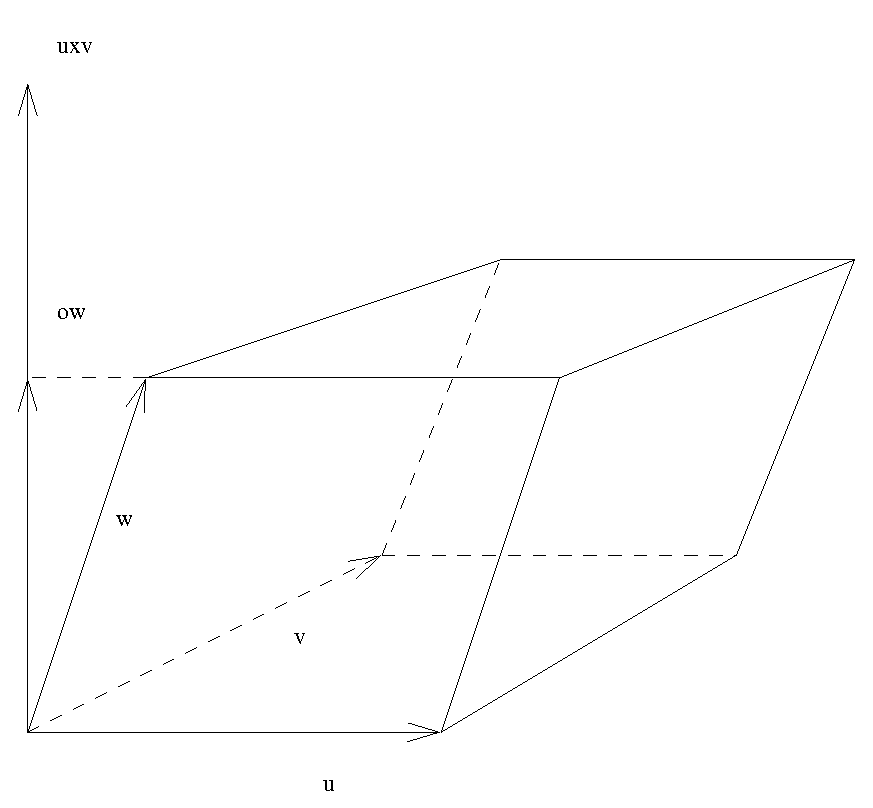
\includegraphics[height=1in]{../../modules/vectors/pictures/ok-volume_box.eps}

\column{0.75\textwidth}
\begin{itemize}
\item $A$, $B$, $C$, $D$ points in space;
\item<2-> $\textbf{u} = \textbf{AB}$, $\textbf{v}=\textbf{AC}$, $\textbf{w}=\textbf{AD}$;
\item<3-> $R=R(\textbf{u},\textbf{v},\textbf{w})$: box on sides $\textbf{u}$, $\textbf{v}$, $\textbf{w}$.\pause
\item<4-> $\text{Vol}(R) = |\textbf{u} \times \textbf{v}| |\textbf{r}| = |\textbf{u} \times \textbf{v}| \, |\textbf{proj}_{\bm{u} \times \bm{v}} \textbf{w}| =
|\textbf{w} \cdot (\textbf{u} \times \textbf{v})|\; .$
\end{itemize}
\end{columns}
\uncover<5->{
\begin{definition}
The quantity $\textbf{w} \cdot (\textbf{u} \times \textbf{v})$ is called the scalar triple product of $\fcv w, \fcv u, \fcv v$.
\end{definition}
}
\uncover<6->{
\begin{itemize}
\item If $\textbf{u} =\langle u_1,u_2,u_3\rangle$,
$\textbf{v} =\langle v_1,v_2,v_3\rangle$, and $\textbf{w} =\langle w_1,w_2,w_3\rangle$, then
%
$$\textbf{w} \cdot (\textbf{u} \times \textbf{v}) = \left|
\begin{array}{ccc}
w_1 & w_2 & w_3 \\
u_1 & u_2 & u_3 \\
v_1 & v_2 & v_3
\end{array}
 \right|$$
\end{itemize}
}
\end{frame}

%\begin{frame}
\frametitle{Use $\times$ to find vector perpendicular to two given}
Recall $\textbf{u} \times \textbf{v}$ is perpendicular to $\textbf{u}$ and $\textbf{v}$.
\begin{example}
Find a vector perpendicular to $\textbf{u} =\langle1,1,0\rangle = \textbf{i}+\textbf{j}$ and $\textbf{v}=\textbf{j}+\textbf{k}=\langle 0,1,1 \rangle$:

\[
\begin{array}{rcl}
 \textbf{w} &= & (\textbf{i}+\textbf{j}) \times (\textbf{j}+\textbf{k}) =
\textbf{i} \times \textbf{j} + \textbf{i} \times \textbf{k} +
\textbf{j} \times \textbf{j} + \textbf{j} \times \textbf{k} = \\
& = & \textbf{k} -\textbf{j}+\textbf{0}+\textbf{i} = \textbf{i} - \textbf{j} + \textbf{k} = \langle1,-1,1\rangle\; .
\end{array}
\]
\end{example}
\end{frame}

\begin{frame}
\frametitle{Use $\times$ to find area of triangle in space}
\begin{columns}
\column{0.3\textwidth}
\psset{xunit=2cm, yunit=2cm}
\begin{pspicture}(-0.3,-0.1)(1.4,1.4)%
\psline[arrows=->](0,0)(1.2,0)%
\psline[arrows=->](0,0)(0.2,1)%
\psline[arrows=->](1.2,0)(0.2,1)%
\psline(0.2,1)(1.4,1)(1.2,0)%
\rput[t](0,-0.1){$A$}
\rput[tl](1.2,-0.1){$B$}
\rput[bl](1.4,1.1){$D$}
\rput[br](0.2,1.1){$C$}
\uncover<2->{%
\rput[l](0.25,0.5){$\fcv w$}%
\fcPerpendicular{[0.2 1]}{[1 0]}{0.1}%
\psline[arrows=->](0.2,0 )(0.2,1)%
}%
\rput[t](0.5, -0.1){$\fcv u$}
\rput[r](0,0.5){$\fcv v$}
\end{pspicture}  
\column{0.7\textwidth}
\begin{itemize}
\item $A$, $B$, $C$ points in space, $\textbf{u} = \textbf{AB}$, $\textbf{v}=\textbf{AC}$. 
\item<2-> Then $|\textbf{w}| = |\textbf{orth}_{\bm{u}} \textbf{v}| = \text{ distance from } C \text{ to } AB\; .$
\item<3-> $|\textbf{u} \times \textbf{v}| = |\textbf{orth}_{\bm{u}} \textbf{v}| \, |\textbf{u}| =
2 \text{area}(ABC) = \text{area}(ABDC)$
\item<4-> $|\textbf{u} \times \textbf{v}|$ = Area of parallelogram on sides $\textbf{u}$ and $\textbf{v}$.
\end{itemize}
%
\end{columns}
\end{frame}

\begin{frame}
\begin{example}
\begin{columns}
\column{0.3\textwidth}
\psset{xunit=0.7cm, yunit=0.7cm}
\begin{pspicture}(-0.1, -1)(4,3.5)
\fcBoundingBox{-0.2}{-1}{4}{3.5}
\fcAxesIIId{3}{3}{3}%
\pscustom*[linecolor=cyan]{%
\fcPolyLineIIId{[1 2 3] [2 3 1] [3 1 2] [1 2 3]}
}
\end{pspicture}
\column{0.7\textwidth}

Find the area of the triangle $A(1,2,3)$, $B(2,3,1)$, $C(3,1,2)$.

\end{columns}
\[\begin{array}{rcl}
\displaystyle \text{Area}(ABC) &=&\displaystyle \frac{1}{2}|\textbf{AB} \times \textbf{AC}| =
\frac{1}{2}|\langle 1,1,-2\rangle \times \langle 2, -1, -1\rangle | \\~\\
&=&\displaystyle\frac{1}{2} |\langle -3, -3, -3 \rangle| \\~\\
&=&\displaystyle \frac{3\sqrt{3}}{2}\; .
\end{array}
\]

\end{example}
\end{frame}

%\begin{frame}[t]
\frametitle{Configurations of pair of lines}
\small
\begin{tabular}{c|r|cccc}
& pair of objects &  \alert<1,2,7,8,13,14,19,20,25,26,31,32,35,36, 39,40>{intersection}&~~\alert<3,4,9,10,15,16,21,22,27,28,37,38,41,42>{parallelism}  ~~& \alert<5,6,11,12,17,18,23,24,29,33,34>{co-planar?} \\\hline
\multirow{3}{*}{\rotatebox{90}{\mbox{2 lines}}}
& \alert<1-6>{intersecting lines} &  \fcAnswer{2}{one point} & \fcAnswer{4}{not parallel} & \fcAnswer{6}{yes}\\
&\alert<7-12>{ parallel lines}& \fcAnswer{8}{empty} & \fcAnswer{10}{parallel} & \fcAnswer{12}{yes} \\
&\alert<13-18>{ skew lines} &\fcAnswer{14}{none} & \fcAnswer{16}{not parallel} &\fcAnswer{18}{no}\\
\hline 
\uncover<19->{
\multirow{3}{*}{\rotatebox{90}{
\begin{tabular}{r}
line \&  \\ plane
\end{tabular}
}}
& \alert<19-24>{line intersecting plane} & \fcAnswer{20}{one point} & \fcAnswer{22}{not parallel} & \fcAnswer{24}{no}\\
& \alert<25-30>{ line parallel to a plane }&\fcAnswer{26}{ none} & \fcAnswer{28}{parallel} & \fcAnswer{30}{no}\\
&\alert<31-34>{ line lying in plane }&\fcAnswer{32}{ line} &-& \fcAnswer{34} {yes} 
\\\hline 
}
\uncover<35->{
\multirow{2}{*}{\rotatebox{90}{\mbox{2 planes}}}
& \alert<35-38>{ intersecting planes} & \fcAnswer{36}{line} & \fcAnswer{38}{not parallel} & - \\
& \alert<39-42>{parallel planes} &\fcAnswer{40}{none} & \fcAnswer{42}{parallel} &~-
}
\end{tabular}

\normalsize
\medskip

\quad \quad \quad 
\psset{xunit=1cm, yunit=1cm}
\begin{pspicture}(-2, -2)(2,2)
\psline[linecolor=black!1](-2.01,-2)(-2,-2) %to give a bounding box
\psline[linecolor=black!1](2.01,2)(2,2)%to give a bounding box
\renewcommand{\fcScreenStyle}{x}
\renewcommand{\fcScreen}{[-1 1 -0.7] -0.25}
\uncover<12,35-38>{\fcParallelogramIIId{[-1 -1 1.5]}{[-1 -1 -1.5]}{[1 1 1.5]}}
\uncover<39->{\fcParallelogramIIId{[-1 -1 1]}{[1 -1 1]}{[-1 1 1]}}

\uncover<6,34>{\fcParallelogramIIId{[-1 -1 0]}{[1 -1 0]}{[-1 1 0]}}

\uncover<1-12,31,33-34>{\fcLineIIId{[-0.8 -0.8 0]}{[0.8 0.8 0]}}
\uncover<32>{\fcLineIIId[linecolor=red]{[-0.8 -0.8 0]}{[0.8 0.8 0]}}

%plane intersection
\uncover<36>{\fcLineIIId[linecolor=red]{[-1 -1 0]}{[1 1 0]}}
\uncover<37,38>{\fcLineIIId{[-1 -1 0]}{[1 1 0]}}

\uncover<1-6,13-18>{\fcLineIIId{[0.8 -0.8 0]}{[0 0 0]}}
\uncover<1-6,13-18>{\fcLineIIId{[0 0 0]}{[-0.8 0.8 0]}}

%\uncover<0>{\fcLineIIId[linestyle=dashed]{[0 0 0]}{[-0.8 0.8 0]}}
 
%bottom plane:
\uncover<6->{\fcPolyLineIIId{[-1 -1 0] [1 -1 0] [1 1 0]}} 
\uncover<6-11,13-34>{\fcPolyLineIIId{[1 1 0] [-1 1 0] [-1 -1 0]}}
\uncover<12,35->{\fcPolyLineIIId[linestyle=dashed]{[1 1 0] [-1 1 0] [-1 -1 0]}}
\uncover<39->{\fcLineIIId{[-1 -1 0]}{[-1 0.3 0]} \fcLineIIId{[1 1 0]}{ [-0.3 1 0]}}

%top parallel plane:
\uncover<39->{\fcPolyLineIIId{[-1 -1 1] [1 -1 1] [1 1 1] [-1 1 1] [-1 -1 1]}}

\uncover<7-18,25-30>{\fcLineIIId{[-0.8 -0.8 1]}{[0.8 0.8 1]}}

\uncover<19-24>{\fcLineIIId[linestyle=dashed]{[-0.8 -0.8 -0.8]}{[0 0 0]}\fcLineIIId{[0 0 0]}{[0.8 0.8 0.8]}}

\uncover<35-38>{\fcPolyLineIIId[linestyle=dashed]{[-1 -1 0] [-1 -1 -1.5] [1 1 -1.5] [1 1 0]}}
\uncover<35-38>{\fcPolyLineIIId{[-1 -1 0] [-1 -1 1.5] [1 1 1.5] [1 1 0]}}

\uncover<2,20>{\fcDotIIId[linecolor=red]{[0 0 0]}}
\uncover<3-6, 21-24>{\fcDotIIId[linecolor=black]{[0 0 0]}}

\end{pspicture}
\end{frame}
%\begin{frame}[label=current]
\frametitle{Euclidean Distance in Coordinates}
\begin{definition}
The distance between the points $A(x_A,y_A,z_A)$ and $B(x_B,y_B,z_B)$ is given by:
\[
d(A,B) = |AB| = \sqrt{(x_B-x_A)^2+(y_B-y_A)^2+(z_B-z_A)^2}
\]
\end{definition}
\begin{columns}
\column{0.4\textwidth}
\psset{xunit=1cm, yunit=1cm}
\begin{pspicture}(-2, -2)(2,2)
\renewcommand{\fcScreen}{[-0.5 1 -0.2] -1}
\tiny
\fcAxesIIId{3}{3}{3}
\fcPolyLineIIId[linecolor=red]{[2.6 1 1][2.6 1.4 1] [3 1.4 1] }
\fcPolyLineIIId[linecolor=red]{[2.8 3.7 1][2.8 3.7 1.360555128] [3 4 1.360555128] }

\fcPolyLineIIId[linestyle=dotted]{ [1 1 1] [1 4 1] [1 4 3]}
\fcLineIIId[linestyle=dotted]{[1 4 1]}{[3 4 1]}
\fcParallelogramHollowIIId{ [1 1 1] }{ [3 1 1] }{ [3 1 3] }
\fcParallelogramHollowIIId{ [1 1 3] }{ [3 1 3] }{ [3 4 3] }
\fcParallelogramHollowIIId{ [3 1 1] }{ [3 4 1] }{ [3 4 3] }
\fcLineIIId[linestyle=dotted]{[1 1 1]}{[3 4 1]}
\fcLineIIId[linestyle=dotted]{[1 1 1]}{[3 4 3]}
\fcPutIIId[t]{[1 1 0.9]}{$A$}
\fcPutIIId[l]{[3 4 3]}{$~~B$}
\fcPutIIId[l]{[3 4 1]}{$~~C$}
\fcPutIIId[t]{[3 1 0.9]}{$D$}

\fcPutIIId[t]{[2 1 0.9]}{$x_B- x_A$}
\fcPutIIId[tl]{[3 2.5 1]}{$~~y_B- y_A$}

\fcPutIIId[l]{[3 4 2]}{$~~z_B- z_A$}
\end{pspicture}
\column{0.6\textwidth}
Motivation. 

Pythagorean theorem for $\triangle ADC$: $|AC|^2 = |AD|^2+|DC|^2$.
Pythagorean theorem for $\triangle ACB$: $|AB|^2 =|AC|^2+ |BC|^2= |AD|^2+|DC|^2+|BC|^2 = (x_B-x_A)^2+(y_B-y_A)^2+(z_B-z_A)^2$.
\end{columns}

%\psfrag{O}{$O$}
%\psfrag{A}{$A$} 
%\psfrag{B}{$B(x_B, y_B, z_B)$}  
%\psfrag{C}{$C(x_B, y_B, z_A)$}    
%\psfrag{x}{$y$} 
%\psfrag{y}{$x$} 
%\psfrag{z}{$z$}     
%\psfrag{dx}{$y_B - y_A$}
%\psfrag{dy}{$x_B - x_A$}
%\psfrag{dz}{$z_B - z_A$}  
%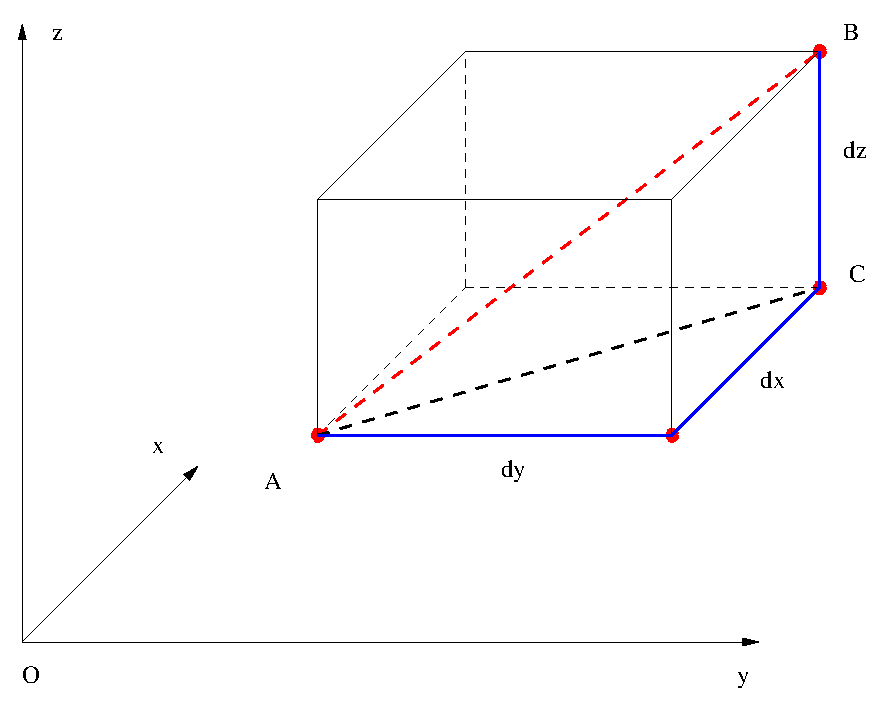
\includegraphics[height=1in]{../../modules/coordinate-systems/pictures/euclidean_distance.eps}
%
%
Example: $P(3,1,2)$ and $Q(1,2,3)$:\pause
%
$$D(P,Q) = \sqrt{(1-3)^2+(2-1)^2+(3-2)^2} = \sqrt{6}\; .$$

\end{frame}

%

\begin{frame}\frametitle{Difference of vectors}
\begin{columns}
\column{0.4\textwidth}
\psset{xunit=1cm, yunit=1cm}
\begin{pspicture}(-0.5,-2.5)(4.1,3.1)%
\fcBoundingBox{-0.5}{-2.5}{4.1}{3.1}
\uncover<1,2,6>{\rput[b](1, 0.6){$\fcv u$}}
\uncover<1,2,6>{\psline[arrows=->](0,0)(2,1)}
\uncover<3>{\psline[arrows=->, linecolor=red](0,0)(2,1)}

\uncover<3-4,7->{\psline[arrows=->, linecolor=red](2,1)(0,0)}
\uncover<5>{\psline[arrows=->](2,1)(0,0)}
\uncover<3>{\rput[lt](1,0.5){$\alert<3>{-\fcv u=\fcv{BA}}$}}
\uncover<4-5,7->{\rput[lt](1,0.5){$\alert<4,7>{-\fcv u}$}}
\uncover<3>{\fcFullDot{0}{0}}
\uncover<6>{\psline[arrows=->](0,0)(1,-2)}
\uncover<7>{\psline[arrows=->, linecolor=red](0,0)(1,-2)}
\uncover<6->{\rput[tr](0.5, -1){$\alert<7>{\fcv v}~$}}
\uncover<1-5>{%
\rput[tl](0,-0.1){$A$}
\rput[tl](2,0.9){$B$}
}%
\uncover<7->{%
\psline[arrows=->, linecolor=red](2,1)(1,-2)
\rput[l](1.5,-0.5){$~~\alert<7>{\fcv v-\fcv u }$}
}
\end{pspicture}
\column{0.6\textwidth}
\begin{itemize}
\item Let $\fcv u=\fcv{AB}$. 
\item<2-> We define $-\fcv u$ to be \uncover<5->{\alert<5>{the}} \uncover<1-4>{a} vector for which $\fcv u +(-\fcv u)=\fcv 0 $. 
\item<3-> Since $\fcv{AB} + \fcv{BA} = \fcv{0}$, it follows $\alert<3>{-\fcv u=\fcv {BA}}$.
\item<4-> In other words $-\fcv{u}$ is depicted using the arrow opposite to $\fcv u$.
\item<5-> From picture, it's evident \alert<5>{$-\fcv u $ can be chosen in a only one way}.
\item<6-> We define the difference of vectors $\fcv v, \fcv u$ via \uncover<7->{$\alert<7>{\fcv{v}-\fcv{u}= (-\fcv{u})+ \fcv{v} } $ (triangle rule).}
\end{itemize}
\end{columns}
\end{frame}
%\begin{frame}
\begin{example}
$\alert<2>{( 1,2,3 ) \cdot ( 6,5,4 ) =} \uncover<3->{\alert<3>{1 \cdot 6 + 2\cdot 5 + 3 \cdot 4 = 28}}$
\end{example}
\end{frame}

\begin{frame}
\begin{example}
\begin{columns}
\column{0.25\textwidth}
\psset{xunit=0.5cm, yunit=0.5cm}
\begin{pspicture}(-2, -2)(3,3)%
\renewcommand{\fcScreen}{[-1 0.8 -0.2] 0}%
\only<6->{\renewcommand{\fcScreen}{[-1 0.571429 -0.2] 0}}
\only<7->{\renewcommand{\fcScreen}{[-1 0.342857 -0.2] 0}}
\only<8->{\renewcommand{\fcScreen}{[-1 0.114286 -0.2] 0}}
\only<9->{\renewcommand{\fcScreen}{[-1  -0.114286 -0.2] 0}}
\only<10->{\renewcommand{\fcScreen}{[-1 -0.342857 -0.2] 0}}
\only<11->{\renewcommand{\fcScreen}{[-1 -0.8 -0.2] 0}}
\fcBoundingBox{-3}{-3}{3}{3}%
\fcAxesIIIdFull{3}{3}{3}%
\uncover<4->{\fcPerpendicularIIId{[1 -2 3]}{[-1 1 1]}{0.4}}%
\fcLineIIId[linecolor=blue,arrows=->]{[0 0 0]}{[1 -2 3]}%
\fcLineIIId[linecolor=blue, arrows=->]{[0 0 0]}{[1 -1 -1]}%
\end{pspicture}
\column{0.75\textwidth}
Are the vectors $( 1,-2,3 ) \cdot ( 1,-1,-1 ) $ perpendicular?

\[
\uncover<2->{\alert<2,3>{ ( 1,-2,3 ) \cdot ( 1,-1,-1 ) =}} \uncover<3->{\alert<3>{1\cdot 1 + (-1)\cdot (-2)+ 3\cdot (-1)=0}},
\]
\uncover<4->{therefore the vectors are perpendicular.}
\uncover<5->{Is this apparent from the picture? Not unless the two vectors lie in a plane parallel to the surface of the page/computer screen.}
\uncover<12>{}
\end{columns}
\end{example}
\end{frame}

%\begin{frame}
\frametitle{Projections in coordinates}
\begin{columns}
\column{0.4\textwidth}
\psset{xunit=0.6cm, yunit=0.6cm}
\begin{pspicture}(-2, -0.5)(5,3.2)
\fcBoundingBox{-2}{-0.5}{5}{3.2}%
\psline[arrows=->](0,0)(4, 2)%
\rput[tl](3, 1.5){$\fcv v$}%
\rput[bl](1, 3){$ \fcv u$}%
\psline[arrows=->, linecolor=blue](0,0)(2,1)%
\rput[tl](1.5, 0.8){$\textbf{proj}_{\fcv v} \fcv u$}%
\psline[arrows=->, linecolor=red](0,0)(! 4 20 sqrt div 2 20 sqrt div)%
\rput[tl](0.5, 0.1){$\widehat{ \fcv {v}}$}%
\psline[arrows=->](0,0)(1,3)%
\fcPerpendicular[linestyle=dashed]{[1 3]}{[4 2]}{0.2}%
\end{pspicture}
\column{0.6\textwidth}
\[
\begin{array}{rcl}
\fcv{u} &=& u_1 \fcv{i} + u_2 \fcv{j} + u_3 \fcv{k} = \langle u_1, u_2, u_3 \rangle\\
\fcv{v}&=&v_1 \fcv{i} + v_2 \fcv{j} + v_3 \fcv{k} = \langle v_1, v_2, v_3 \rangle
\end{array}
\]
\end{columns}
\uncover<2->{
\begin{theorem}
$\begin{array}{rcl}
\displaystyle\alert<6>{ {\bf comp}_{\fcv v} \fcv u}&\alert<6>{=}& \displaystyle \alert<6>{\frac{\alert<3>{\fcv{u}\cdot \fcv{v}} }{\alert<4>{|\fcv{v}|}}} =\frac{ \alert<3>{ u_1v_1 +u_2v_2+u_3v_3} }{\alert<4>{ \sqrt{v_1^2+v_2^2+v_3^2}}}\\~\\
\displaystyle \alert<5>{{\bf proj}_{\fcv v} \fcv u }&\alert<-1>{=}&\displaystyle \alert<5>{\left(\alert<6>{ {\bf comp}_{\fcv v} \fcv{u}}\right) \alert<7>{\widehat{\fcv v}}} = \alert<6>{\frac{\fcv{u}\cdot \fcv{v}}{|\fcv{v}|}} \alert<7>{ \frac{\fcv v}{|\fcv v|}} = \frac{\fcv{u}\cdot \fcv{v}}{\alert<8>{ |\fcv{v}|^2}}\fcv v= \frac{\fcv u \cdot \fcv v}{\alert<8>{ \fcv v\cdot  \fcv v} }\fcv v
\quad .
\end{array}
$
\end{theorem}
}
\end{frame}

%\begin{frame}
\begin{example}
Let $\fcv u=( 1,2,3)$, $\fcv v=( 6,5,4 )$.
\begin{itemize}
\item Compute the scalar projection $\text{comp}_{\fcv v} \fcv u$ of $\fcv u$ onto $\fcv v$.
\item Compute the vector projection ${\bf proj}_{\fcv v} \fcv u$ of $\fcv u$ onto $\fcv v$.
\item Compute the orthogonal component ${\bf orth}_{\fcv v}\fcv u$.
\end{itemize}

$
\begin{array}{r@{}c@{}l}
\uncover<2->{\displaystyle\text{comp}_{\fcv v}\fcv u&~=~& \displaystyle \frac{\fcv u\cdot \fcv v}{|\fcv v|} \\~\\}
\uncover<2->{\displaystyle\alert<2,3>{ \text{comp}_{( 6,5,4)} ( 1,2,3) }&\alert<2,3>{~=~}& \uncover<3->{\alert<3>{\displaystyle \frac{ (6, 5,4)\cdot(1,2,3)}{\sqrt{( 6, 5, 4 )\cdot ( 6, 5 ,4 )}} = \frac{6\cdot 1 + 5\cdot 2 + 4\cdot 3}{\sqrt{6^2+5^2+4^2}} = \frac{28}{\sqrt{77}}}} \\~\\}
\uncover<4->{ {\bf proj}_{\fcv{v}} \textbf{u} &~=~&\displaystyle \frac{\fcv{u} \cdot \fcv{v}}{|\fcv{v}|^2} \fcv{v}\\~\\}
\uncover<4->{\alert<4,5>{ {\bf proj}_{( 6,5,4)} ( 1,2,3) }& \alert<4,5>{~ =~}&\uncover<5->{\alert<5>{ \frac{28}{77} ( 6,5,4) = \left(\frac{24}{11}, \frac{20}{11}, \frac{16}{11}\right)}} \\}
\uncover<6->{\alert<6,7>{{\bf orth}_{( 6,5,4)} ( 1,2,3)} &\alert<6,7>{~=~}& \uncover<7->{\alert<7>{( 1,2,3) -
\textbf{proj}_{( 6,5,4)} ( 1,2,3)= \left(-\frac{13}{11}, \frac{2}{11}, \frac{17}{11}\right) }}}
\end{array}
$
\end{example}
\end{frame}


%\begin{frame}
\frametitle{Definition of vector}

\begin{columns}
\column{0.3\textwidth}
\centering
\begin{pspicture}(-0.3,-0.5)(1.5,1.2)
\fcBoundingBox{-0.2}{-0.3}{1.1}{1.1}
\fcFullDotBlack{0}{0}
\uncover<1-2>{\fcFullDot{1}{1}}
\rput[tl](1.1,0.9){\alertNoH{1}{$\bm v$}}
\rput[t](0,-0.1){\alertNoH{2,4}{$O$}}
\uncover<3>{\psline[arrows=->, linecolor=red](0, 0)(1,1)}
\uncover<4->{\psline[arrows=->](0, 0)(1,1)}
\uncover<4>{\fcFullDot{0}{0}}
\end{pspicture}
\column{0.7\textwidth}
\begin{itemize}
\item A \alertNoH{1}{\emph{position vector $\fcv{v}$}} (simply - \alertNoH{1}{\emph{vector}}) is a point in a space where there's a fixed preferred point $O$.
\item<2-> \alertNoH{2}{Preferred point $O$} is called the \alertNoH{2}{origin}. 
\item<3-> If not given by $O$, vector is depicted by arrow from $O$ to defining point.
\item<4-> Vector given by origin = zero vector $\fcv{0}$.
\end{itemize}
\end{columns}
\begin{itemize}
\item<5-> Points \& vectors can be identified but:
\begin{itemize}
\item<5-> use term ``vector'' $\Rightarrow$ space has preferred origin point;
\item<7-> if we specifically allow point/vector addition we use the term ``vector'' instead of ``point'';
\item<8-> when we do not intend to carry out addition operations we use the term ``point'' instead of ``vector''.
\end{itemize}
\item<6-> We will soon equip vectors with two operations, vector addition and multiplication by scalars.
\end{itemize}
\end{frame}
%\begin{frame}
\frametitle{Displacement Vectors}
\begin{columns}\column{0.3\textwidth}
\begin{pspicture}(-0.2,-1.1)(2.1,1.1)
\fcBoundingBox{-0.2}{-1.1}{2.1}{1.1}
\fcFullDot{2}{1}
\fcFullDot{1}{-1}
\fcFullDotBlack{0}{0}
\psline(2, 1)(1,-1)
\psline[arrows=->](2, 1)(1,-1)
\end{pspicture}
\column{0.7\textwidth}
\begin{definition}
A displacement vector is an ordered pair of points, $(A,B)$.
\end{definition}
\end{columns}
\begin{itemize}
\item Represented as arrow, $A$ - tail $B$- head
\item Extra notation $(A,B) = \overrightarrow{AB} = \textbf{AB}$
\item Magnitude: $|\textbf{AB}| = |\overrightarrow{AB}|$. 
\item If $A\neq B$ direction is defined as the ray starting at $A$ and passing through $B$.
\item If $A=B$:
\begin{itemize}
\item Zero magnitude and non-specified direction
\item $(A,A) = \overrightarrow{AA} = \textbf{AA}$: zero displacement vector.
\end{itemize}
  \item Displacement vector with tail fixed at $O$:
  \begin{itemize}
    \item Position vector with respect to $O$;
    \item $(O,P) = \overrightarrow{OP} = \textbf{OP} = \textbf{r}_P$.
  \end{itemize}
\end{itemize}
\end{frame}
%\begin{frame}
\frametitle{Position vectors}

  \begin{itemize}
   \item Vector $\textbf{u}$: \\
      set of displacement vectors with given direction and magnitude

    \item  Magnitude of $\textbf{u}$: common given magnitude.

    \item Direction of $\textbf{u}$: common given direction, if non-zero magnitude.

    \item Set of zero displacement vectors = zero vector, $\textbf{0}$. \pause

    \item Representative for $\textbf{u}$: \\
      displacement vector $\textbf{AB}$ with the same direction and magnitude

\begin{figure}[h]
  \psfrag{A}{$A$}
  \psfrag{B}{$B$}
  \psfrag{C}{$C$}
  \psfrag{D}{$D$}
  \psfrag{E}{$E$}
  \psfrag{F}{$F$}
  \psfrag{u}{$\textbf{u}$}
  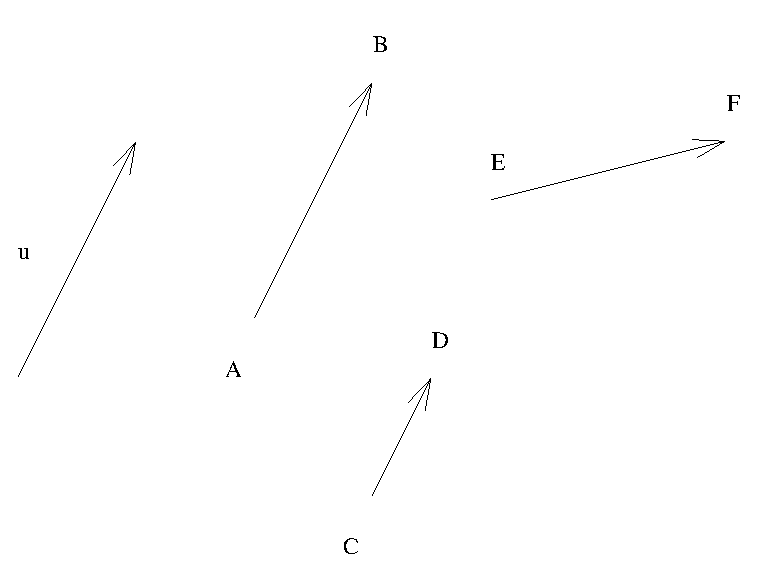
\includegraphics[height=1in]{../../modules/vectors/pictures/ok-vector_representatives.eps}
  \label{fig:vector_representative}

\end{figure}

    \item Intuitive notation:  $\textbf{u}=\textbf{AB}$.

    \item Graphical representation: arrow without fixed tail and head.

    %\item Major advantage: we can translate displacement vectors.
  \end{itemize}
\end{frame}
%\begin{frame}
\frametitle{Equality and Equivalence of Displacement Vectors}
\begin{itemize}
\item<1-> We define two displacement vectors to be equal if:
\[ 
\textbf{AB} = \textbf{DC}  \Longleftrightarrow A=D \text{ and } B=C
\]
\item<2-> Equal displacement vectors $\rightarrow$ same magnitude and direction.
\item<3-> Same magnitude and direction $\not\rightarrow$ equal displacement vectors. 

\item<4-> We define two displacement vectors to be \alert<4>{equivalent} if they have the \alert<4>{same magnitude and direction}. We write $\alert<4>{\textbf{AB} \equiv \textbf{DC}}$.
\item 
\[ 
\textbf{AB} \equiv \textbf{DC} \Longleftrightarrow ABCD \text{ is a parallelogram}\;.
\]
\end{itemize}
\end{frame}
%\begin{comment}
\begin{frame}
\frametitle{Addition of Vectors}
\begin{columns}
\column{0.25\textwidth}
\psset{xunit=1cm, yunit=1cm}
\begin{pspicture}(-0.5,-0.5)(3.1,3.1)%
\tiny
\fcBoundingBox{-0.5}{-0.5}{3.1}{3.1}
\uncover<1>{\psline[arrows=->](0,0)(1,2)}
\uncover<1>{%
\rput[r](0.4, 1){$\bm v$}%
}
\psline[arrows=->](0, 0)(2, 1)%
\rput[t](1, 0.4){$\bm u$}%
\uncover<2>{
\psline[linecolor=gray, arrows=->](0, 0)(1, 2)%
}
\uncover<2->{%
\psline[arrows=->](2,1)(3,3)%
\rput[l](2.6, 2){$\bm v$}}
\uncover<3->{%
\psline[arrows=->](0,0)(3,3)
\rput[rb](1.4,1.5){$\bm u+\bm v$}
}
\end{pspicture}

\column{0.75\textwidth}
\begin{itemize}
\item<1-> \textbf{Triangle Rule.} Define sum of position vectors $\bm u$ and $\bm v$ as follows. 
\item<2-> Attach representative displacement vectors head to tail.
\item<3-> Declare the sum to be the position vector with the tail of the first displacement vector and the head of the second displacement vector.
\end{itemize}
\end{columns}
\end{frame}

\begin{frame}
\frametitle{Properties of addition}
\begin{columns}
\column{0.4\textwidth}
\psset{xunit=1cm, yunit=1cm}
\begin{pspicture}(-0.5,-0.5)(3.1,3.1)%
\tiny
\fcBoundingBox{-0.5}{-0.5}{3.1}{3.1}
\uncover<2-4>{\psline[arrows=->, linecolor=red](0,0)(1,2)}
\uncover<5->{\psline[arrows=->](0,0)(1,2)}
\uncover<2->{\rput[r](0.4, 1){$\alert<2-4>{\bm v}$}}
\psline[arrows=->](2,1)(3,3)%
\uncover<1>{\psline[arrows=->, linecolor=red](2,1)(3,3)}
\rput[l](2.6, 2){$\alert<1>{\bm v}$}

\psline[arrows=->](0, 0)(2, 1)%
\uncover<1>{\psline[arrows=->, linecolor=red](0, 0)(2, 1)}
\rput[t](1, 0.4){$\alert<1>{\bm u}$}%
\uncover<3,4>{\psline[arrows=->, linecolor=red](1,2)(3,3)}
\uncover<5->{\psline[arrows=->](1,2)(3,3)}
\uncover<3->{\rput[b](2, 2.6){$\alert<3,4>{\bm u}$}}
\psline[arrows=->](0,0)(3,3)
\uncover<1,4>{
\psline[arrows=->, linecolor=red](0,0)(3,3)
}
\uncover<4->{\rput[t](1.62,1.62){\rotatebox{45}{$\alert<4>{ \bm v+\bm u}$}}}
\rput[b](1.38,1.38){\rotatebox{45}{$\alert<1>{\bm u+\bm v}$}}
\end{pspicture}

\uncover<5->{
\psset{xunit=0.8cm, yunit=0.8cm}
\begin{pspicture}(-0.5, -1)(4, 4)
\fcBoundingBox{-0.5}{-1}{4}{4}
\tiny

\uncover<5->{\psline[arrows=->](0,0)(0.5, 2) }
\uncover<6,9>{\psline[arrows=->, linecolor=red](0,0)(0.5,2)}
\rput[r](0.15,1){$\alert<6,9>{\bm u}$}

\uncover<5->{\psline[arrows=->](0.5, 2)(3, 3)}
\uncover<6,8>{\psline[arrows=->, linecolor=red](0.5,2)(3,3)}
\rput[b](1.75,2.6){$\alert<6,8>{\bm v}$}

\uncover<6->{\rput[tl](1.7, 1.7){\alert<6,7>{$\bm u+\bm v$}}}
\uncover<6,7>{\psline[arrows=->, linecolor=red](0,0)(3,3)}
\uncover<8->{\psline[arrows=->](0,0)(3,3)}

\uncover<7>{\psline[arrows=->, linecolor=red](3,3)(4,0)}

\uncover<5->{\psline[arrows=->](3, 3)(4, 0)}
\uncover<7,8>{\psline[arrows=->, linecolor=red](3, 3)(4, 0)}
\rput[lb](3.6,1.5){$\alert<7,8>{\bm w}$}

\uncover<7->{\rput[t](2, -0.1){\alert<6,7,10>{$(\bm u+\bm v )+\bm w$}}}
\uncover<9->{\rput[b](2, 0.1){\alert<9,10>{$\bm u+(\bm v +\bm w)$}}}
\uncover<8,11->{\psline[arrows=->](0, 0)(4, 0)}
\uncover<7,9,10>{\psline[arrows=->, linecolor=red](0, 0)(4, 0)}


\uncover<8->{\rput[tr](2.25, 1){$\alert<8,9>{\bm v+\bm w}$}}
\uncover<10->{\psline[arrows=->](0.5, 2)(4,0)}
\uncover<8,9>{\psline[arrows=->, linecolor=red](0.5, 2)(4,0)}

\end{pspicture}
}
\column{0.6\textwidth}
\begin{itemize}
\item Addition is commutative (parallelogram rule): \[ \alert<1>{\bm{u}+ \bm{v}} = \alert<4>{\alert<2>{\bm{v}}+ \alert<3>{\bm{u}}}.\]

\item<5-> Addition is associative: 
\[
\alert<10>{\alert<7>{(\alert<6>{ \bm{u}+\bm{v}})+\bm{w} } = \alert<9>{\bm{u} + (\alert<8>{ \bm{v} + \bm{w}})}}
\] 

\item<11-> As usual we write $\bm{u}+\bm{v}+\bm{w}=( \bm{u} +\bm{v})+\bm{w}= \bm{u}+(\bm{v}+\bm{w})$.
\end{itemize}
\end{columns}
\end{frame}
\end{comment}


\begin{frame}\frametitle{Difference of vectors}
\begin{columns}
\column{0.4\textwidth}
\psset{xunit=1cm, yunit=1cm}
\begin{pspicture}(-0.5,-2.5)(4.1,3.1)%
\fcBoundingBox{-0.5}{-2.5}{4.1}{3.1}
\uncover<1,2,6>{\rput[b](1, 0.6){$\bm u$}}
\uncover<1,2,6>{\psline[arrows=->](0,0)(2,1)}
\uncover<3>{\psline[arrows=->, linecolor=red](0,0)(2,1)}

\uncover<3-4,7->{\psline[arrows=->, linecolor=red](2,1)(0,0)}
\uncover<5>{\psline[arrows=->](2,1)(0,0)}
\uncover<3>{\rput[lt](1,0.5){$\alert<3>{-\bm u=\bm{BA}}$}}
\uncover<4-5,7->{\rput[lt](1,0.5){$\alert<4,7>{-\bm u}$}}
\uncover<3>{\fcFullDot{0}{0}}
\uncover<6>{\psline[arrows=->](0,0)(1,-2)}
\uncover<7>{\psline[arrows=->, linecolor=red](0,0)(1,-2)}
\uncover<6->{\rput[tr](0.5, -1){$\alert<7>{\bm v}~$}}
\uncover<7->{\psline[arrows=->, linecolor=red](2, 1)(1,-2)}
\uncover<7->{\rput[l](1.5,-0.5){$~\alert<7>{\bm v-\bm u}$}}
\uncover<1-5>{
\rput[tl](0,-0.1){$A$}
\rput[tl](2,0.9){$B$}
}
\end{pspicture}
\column{0.6\textwidth}
\begin{itemize}
\item Let $\bm u=\bm{AB}$. 
\item<2-> We define $-\bm u$ to be \uncover<5->{\alert<5>{the}} \uncover<1-4>{a} vector for which $\bm u +(-\bm u)=\bm 0 $. 
\item<3-> Since $\bm{AB} + \bm{BA} = \bm{0}$, it follows $\alert<3>{-\bm u=\bm {BA}}$.
\item<4-> In other words $-\bm{u}$ is depicted using the arrow opposite to $\bm u$.
\item<5-> From picture, it's evident \alert<5>{$-\bm u $ can be chosen in a only one way}.
\item<6-> We define the difference of vectors $\bm v, \bm u$ via \uncover<7->{$\alert<7>{\bm{v}-\bm{u}= (-\bm{u})+ \bm{v} } $ (triangle rule)}.
\end{itemize}
\end{columns}
\end{frame}
%\begin{frame}
\frametitle{Linear Combinations}
\begin{columns}
\column{0.3\textwidth}
\psset{xunit=0.6cm, yunit=0.6cm}
\begin{pspicture}(-2,-2)(3.1,3.3)
\fcBoundingBox{-2}{-2}{3}{3}
\fcFullDot{0}{0}
\rput[br](3, 3){$\fcv u$}
\psline[arrows=->](0,0)(3,3)
\uncover<handout:0|3>{
\psline[arrows=->, linecolor=red](0,0)(1.5,1.5)
\rput[tl](0.75, 0.75){$\alertNoH{3}{\frac{1}{2}\fcv u}$}
}
\uncover<4>{
\psline[arrows=->, linecolor=red](0,0)(2,2)
\rput[tl](1, 1){$\alertNoH{4}{\frac{2}{3}\fcv u}$}
}
\uncover<handout:0|5>{
\psline[arrows=->, linecolor=red](0,0)(1,1)
\rput[tl](0.5, 0.5){$\alertNoH{5}{\frac{1}{3}\fcv u}$}
}
\uncover<6>{
\psline[arrows=->, linecolor=red](0,0)(-2,-2)
\rput[tl](-1, -1){$\alertNoH{6}{-\frac{1}{2}\fcv u}$}
}
\end{pspicture}
\column{0.7\textwidth}
\begin{itemize}
\item<1-> Let $\fcv{u}$ be vector, $c$ be a real number (scalar).
\item<2-> Define \alertNoH{2}{the product of the vector $\fcv u$ and the scalar $c$} as follows.
\begin{itemize}
\item<2-> If $c >0$ define $c\fcv{u}$ as the vector:
\begin{itemize}
\item with the same direction
\item with magnitude proportional with coefficient $c$ to the magnitude of $\fcv u$, i.e., $|c\fcv{u}| = c|\fcv{u}|$.
\end{itemize}

\item<6-> If $c<0$ define $c\fcv{u}$ as the vector $(-c)(-\fcv{u})$, i.e, as the vector:
\begin{itemize}
\item with opposite direction
\item with magnitude $|c\fcv{u}| = |(-c)(-\fcv{u})| = (-c)|-\fcv{u}| = |c||\fcv{u}|$
\end{itemize}
\item<7-> If $c=0$ then define $c\fcv u=0\fcv{u} = \fcv{0}$.
\end{itemize}
\end{itemize}
\end{columns}
\begin{itemize}
\item If $c_1, \ldots , c_n$ are scalars and $\fcv{u}_1,\ldots, \fcv{u}_n$ are vectors, we say
\[
\fcv{v} = c_1\fcv{u}_1+ \dotsb + c_n \fcv{u}_n
\]
is a \emph{linear combination} of the vectors $\fcv u_1,\dots, \fcv u_n$.
\end{itemize}
\end{frame}
%\begin{frame}
  \frametitle{Decomposition of a vector along given directions}

  Example: Tension induced by given force.

\begin{figure}[h]
  \psfrag{F}{$\textbf{F}$}
  \psfrag{-F}{$-\textbf{F}$}
  \psfrag{F1}{$\textbf{F}_1$}
  \psfrag{F2}{$\textbf{F}_2$}
  \psfrag{T1}{$\textbf{T}_1$}
  \psfrag{T2}{$\textbf{T}_2$}
  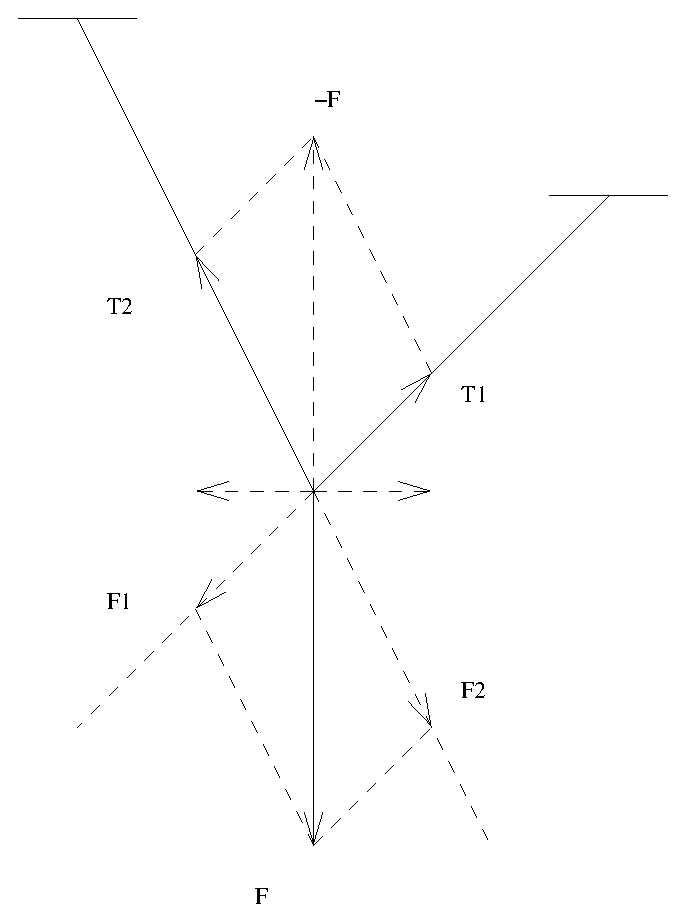
\includegraphics[height=2in]{../../modules/vectors/pictures/ok-tension.eps}
  \label{fig:tension}
  %\caption{Decomposition of a vector}
\end{figure}


\end{frame}
%%\begin{comment}
\begin{frame}
\frametitle{Vectors in Coordinates}
\begin{columns}
\column{0.3\textwidth}
\psset{xunit=0.7cm, yunit=0.7cm}
\begin{pspicture}(-0.5 ,-2)(4.5, 4)
\fcBoundingBox{-0.5}{-2}{4.5}{4}
\tiny
\renewcommand{\fcScreen}{[-1 1.1 -0.5] 0}
\fcAxesIIId{3}{3}{3}
\fcPutIIId[r]{[0 0 0]}{$O~$}
\uncover<3->{
\fcLineIIId[arrows=->, linecolor=red]{[0 0 0]}{[1 0 0]}
\fcLineIIId[arrows=->, linecolor=red]{[0 0 0]}{[0 1 0]}
\fcLineIIId[arrows=->, linecolor=red]{[0 0 0]}{[0 0 1]}
\fcPutIIId[t]{[0.5 0 -0.1]}{$\alert<3>{\bm i}$}
\fcPutIIId[br]{[0 0.5 0]}{$\alert<3>{\bm j}$}
\fcPutIIId[r]{[0 0 0.5]}{$\alert<3>{\bm k}~~$}
}
\uncover<5->{
\fcPutIIId[lb]{[2.5 2.5 2.8]}{$U\uncover<6->{(a,b,c)}$}
\fcDotIIId[linecolor=blue]{[2.5 2.5 2.5]}%
\fcLineIIId[arrows=->, linecolor=red]{[0 0 0]}{[2.5 2.5 2.5]}
}
\uncover<2,3>{
\fcDotIIId{[1 0 0]}
\fcDotIIId{[0 1 0]}
\fcDotIIId{[0 0 1]}
}
\uncover<2>{
\fcPutIIId[t]{[1 0 -0.2]}{\alert<2>{$I$}}
\fcPutIIId[br]{[0 1 0]}{\alert<2>{$J~~$}}
\fcPutIIId[r]{[0 0 1]}{\alert<2>{$K~~$}}
}
\uncover<6,11>{
\fcLineIIId[linecolor=gray]{[2.5 2.5 2.5]}{[2.5 2.5 0]}
\fcLineIIId[linecolor=gray]{[2.5 2.5 2.5]}{[2.5 0 2.5]}
\fcLineIIId[linecolor=gray]{[2.5 2.5 2.5]}{[0 2.5 2.5]}
\fcLineIIId[linecolor=gray]{[0 2.5 2.5]}{[0 0 2.5]}
\fcLineIIId[linestyle=dashed, linecolor=gray]{[0 2.5 2.5]}{[0 2.5 0]}
\fcLineIIId[linecolor=gray]{[2.5 0 2.5]}{[0 0 2.5]}
\fcLineIIId[linecolor=gray]{[2.5 0 2.5]}{[2.5 0 0]}
\fcLineIIId[linestyle=dashed, linecolor=gray]{[2.5 2.5 0]}{[0 2.5 0]}
\fcLineIIId[linecolor=gray]{[2.5 2.5 0]}{[2.5 0 0]}%
}
\uncover<6>{
\fcPutIIId[t]{[1.25 0 -0.1]}{$a$}
\fcPutIIId[b]{[0 1.25 0.1]}{$b$}%
\fcPutIIId[r]{[0 0 1.25]}{$c~~$}%
}
\uncover<8->{
\fcPutIIId[t]{[1.25 0 -0.1]}{$a\bm{i}$}
\fcLineIIId[arrows=->, linecolor=red]{[0 0 0]}{[2.5 0 0]}
}
\uncover<9->{
\fcLineIIId[arrows=->, linecolor=red]{[2.5 0 0]}{[2.5 2.5 0]}
\fcPutIIId[lt]{[2.5 1.25 0]}{$~b\bm{j}$}%
}
\uncover<10->{
\fcLineIIId[arrows=->, linecolor=red]{[2.5 2.5 0]}{[2.5 2.5 2.5]}
\fcPutIIId[l]{[2.5 2.5 1.25]}{$~c\bm{k}$}%
}
\end{pspicture}
\column{0.7\textwidth}
\begin{itemize}
\item<1-> Fix coordinate system $Oxyz$.
\item<2-> Let $I$, $J$, $K$ be the points giving the units on the $x,y,z$ axes as indicated.
\item<3-> Define $\bm{i}$, $\bm{j}$, $\bm{k}$ to be the unit vectors $\bm{OI}$, $\bm{OJ}$, $\bm{OK}$.
\end{itemize}
\end{columns}
\begin{itemize}
\item<5-> Let $\bm u= \bm{OU}$ be a vector.
\item<6-> Let $U$ have coordinates $(a,b,c)$.
\item<7-> Then $\bm u =\alert<10>{ \alert<9>{\alert<8>{ a\bm{i}}+b\bm{j}}+c\bm{k} }$.
\item<8-11> This follows from the point-vector identification.
\end{itemize}
\end{frame}
%\end{comment}
\begin{frame}
\begin{columns}
\column{0.3\textwidth}
\psset{xunit=0.7cm, yunit=0.7cm}
\begin{pspicture}(-0.5 ,-2)(4.5, 4)
\fcBoundingBox{-0.5}{-2}{4.5}{4}
\tiny
\renewcommand{\fcScreen}{[-1 1.1 -0.5] 0}
\fcAxesIIId{3}{3}{3}
\fcPutIIId[r]{[0 0 0]}{$O~$}
\fcLineIIId[arrows=->, linecolor=red]{[0 0 0]}{[1 0 0]}
\fcLineIIId[arrows=->, linecolor=red]{[0 0 0]}{[0 1 0]}
\fcLineIIId[arrows=->, linecolor=red]{[0 0 0]}{[0 0 1]}
\fcPutIIId[t]{[0.5 0 -0.1]}{$\alert<3>{\bm i}$}
\fcPutIIId[br]{[0 0.5 0]}{$\alert<3>{\bm j}$}
\fcPutIIId[r]{[0 0 0.5]}{$\alert<3>{\bm k}~~$}
\fcPutIIId[lb]{[2.5 2.5 2.8]}{$U(a,b,c)$}
\uncover<2->{\fcPutIIId[rb]{[1.25 1.25 1.3]}{$\bm u( a,b,c)$}}
\fcDotIIId[linecolor=blue]{[2.5 2.5 2.5]}%
\fcLineIIId[arrows=->, linecolor=red]{[0 0 0]}{[2.5 2.5 2.5]}
\fcPutIIId[t]{[1.25 0 -0.1]}{$a\bm{i}$}
\fcLineIIId[arrows=->, linecolor=red]{[0 0 0]}{[2.5 0 0]}
\fcLineIIId[arrows=->, linecolor=red]{[2.5 0 0]}{[2.5 2.5 0]}
\fcPutIIId[lt]{[2.5 1.25 0]}{$~b\bm{j}$}%
\fcLineIIId[arrows=->, linecolor=red]{[2.5 2.5 0]}{[2.5 2.5 2.5]}
\fcPutIIId[l]{[2.5 2.5 1.25]}{$~c\bm{k}$}%
\end{pspicture}
\column{0.7\textwidth}
\begin{itemize}
\item<1-> From preceding: arbitrary vector $\bm u= \bm {OU}$ can be decomposed as $\bm u= a\bm i+b\bm j + c\bm k$, where $(a,b,c)$: Cartesian coordinates of $U$.
\item<2-> Thus $\bm u$ is identified with the triple of numbers $( a, b, c)$.
\end{itemize}
\end{columns}

\begin{itemize}
\item<3-> Under the first definition of vector, a vector is simply a point in a vector space (=space with a distinguished point).
\item<4-> From now on, we assume the first definition of vector: we use the notation $(a,b,c)$ both for points in vector spaces (vectors) and points in spaces not equipped with vector space structure.
\item<5-> Under the second alternative definition of vector, there is a formal distinction between points and vectors.
\item<6-> Some authors who use the second definition use the notation $\langle a, b, c \rangle$ to denote vectors and $(a,b,c)$ to denote points.
\end{itemize}
\end{frame}

%\begin{frame}
\frametitle{Work done by a constant force}
\only<1>{
\begin{figure}[h]
  \psfrag{F}{$\textbf{F}$}
  \psfrag{O}{$O$}
  \psfrag{P}{$P$}
  \psfrag{a}{$\alpha$}
  \psfrag{pvF}{$\textbf{proj}_{\bm{v}} \textbf{F}$}
  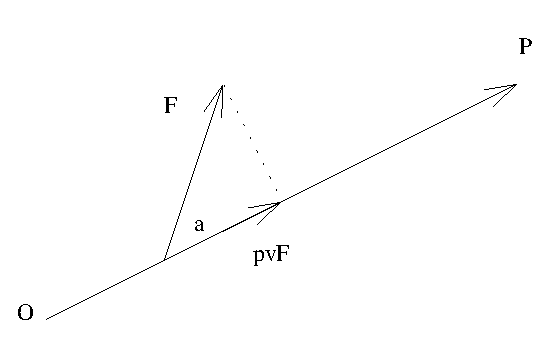
\includegraphics[height=2in]{../../modules/vectors/pictures/ok-positive_work.eps}
\end{figure}

$$W = |\textbf{proj}_{\bm{v}} \textbf{F}| \, |\textbf{OP}| =|\textbf{F}| \, |\textbf{OP}|\, \cos{\alpha}\; .$$
}

\only<2>{
\begin{figure}[h]
  \psfrag{F}{$\textbf{F}$}
  \psfrag{O}{$O$}
  \psfrag{P}{$P$}
  \psfrag{a}{$\alpha$}
  \psfrag{pvF}{$\textbf{proj}_{\bm{v}} \textbf{F}$}
  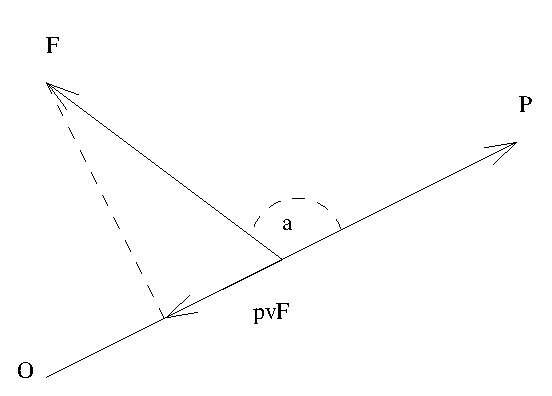
\includegraphics[height=2in]{../../modules/vectors/pictures/ok-negative_work.eps}
\end{figure}

$$W = - |\textbf{proj}_{\bm{v}} \textbf{F}| \, |\textbf{OP}| = |\textbf{F}| |\textbf{OP}| \cos{\alpha}\; .$$
}

\end{frame}


%\begin{frame}
\frametitle{Dot Product}
\begin{columns}
\column{0.5\textwidth}
\begin{pspicture}(-0.5, -0.5)(5,3.2)
\fcBoundingBox{-0.5}{-0.5}{5}{3.2}
\psline[arrows=->](0,0)(4, 2)
\rput[tl](3, 1.5){$\bm v$}
\rput[tl](0.5, 0.2){$\hat{ \bm {v}}$}
\rput[bl](1, 3){$ \bm u$}
\rput[r](-0.5, 1){$\textbf{orth}_{\bm v} \bm u$}

\rput[r](-0.5, 1){$\textbf{orth}_{\bm v} \bm u$}
\rput[tl](1.5, 0.8){$\textbf{proj}_{\bm v} \bm u$}

\psline[arrows=->](0,0)(2,1)
\psline[arrows=->, linecolor=red](0,0)(! 4 20 sqrt div 2 20 sqrt div)

\psline[arrows=->](0,0)(1,3)
\psline[arrows=->](0,0)(! -1 2)
\fcPerpendicular[linestyle=dashed]{[1 3]}{[4 2]}{0.2}%
\fcPerpendicular[linestyle=dashed]{[1 3]}{[-2 4]}{0.2}%
\fcAngle{0.463648}{ 1.249046 }{0.4}{$\alpha$}
\end{pspicture}
\column{0.5\textwidth}

\begin{itemize}
\item<1-> Let $\bm{u}$, $\bm{v}$ vectors, $\bm{v}\neq \bm{0}$.

\item<2-> Let $\textbf{proj}_{\bm{v}} \bm{u}$: projection of $\bm{u}$ along $\bm{v}$.

\item<3-> Let $\textbf{orth}_{\bm{v}} \bm{u}$: projection of $\bm{u}$ orthogonal to $\bm{v}$.

\item<4-> Then $\hat{\bm{v}} = \frac{1}{|\bm{v}|} \bm{v}$ is the unit vector along $\bm{v}$.

\item<5-> Let $\alpha$: angle between $\bm v$ and $\bm u$.

\item<6-> Then $\textbf{proj}_{\bm{v}} \bm{u} =  \cos \alpha |\bm{u}| \hat{\bm{v}}$.

\item<7-> Define dot product of $u$ and $v$:
\[
\bm{u} \cdot \bm{v} =  \cos \alpha |\bm u||\bm{v}| .
\]
\end{itemize}
\end{columns}
\end{frame}

%\begin{frame}
 \frametitle{Properties of Dot Product}

  \begin{itemize}
   \item If $\textbf{v}=\textbf{0}$ or $\textbf{u}=\textbf{0}$, then $\textbf{u}\cdot \textbf{v} =0$.

  \item If $\textbf{u} \neq 0 \neq \textbf{v}$, then $comp_{\bm{v}} \textbf{u} = |\textbf{u}|\cos{\alpha}$
%
$$\textbf{u} \cdot \textbf{v} = |\textbf{u}| \, |\textbf{v}|\,\cos{\alpha}$$
%
\item If $\textbf{u}\neq \textbf{0} \neq \textbf{v}$, then
%
$$\textbf{u} \cdot \textbf{v} = 0 \Longleftrightarrow \textbf{u} \bot \textbf{v}\; .$$
%
\item $\textbf{u} \cdot \textbf{v} = (\textbf{proj}_{\bm{v}} \textbf{u}) \cdot \textbf{v}$

\item The dot product is linear in each argument:
%
$$ (a \textbf{u} + b \textbf{w}) \cdot \textbf{v} = a \textbf{u} \cdot \textbf{v} + b \textbf{w} \cdot \textbf{v}$$
%
$$ \textbf{u} \cdot (a \textbf{v} + b \textbf{w}) = a \textbf{u} \cdot \textbf{v} + b \textbf{u} \cdot \textbf{w}$$

\item Dot product is positive definite:
%
$$\textbf{v} \cdot \textbf{v} = |\textbf{v}|^2 \geqslant 0 \text{ and }
\textbf{v}\cdot \textbf{v} = 0 \leftrightarrow \textbf{v}=\textbf{0}$$
  \end{itemize}

\end{frame}
%\begin{frame}
 \frametitle{Computations in Coordinates}

 \begin{itemize}
  \item  $Oxyz$: rectangular coordinate system

  \item $\textbf{i}$, $\textbf{j}$, $\textbf{k}$: unit vectors along fundamental directions.
%
$$ \textbf{i} \cdot \textbf{j} = \textbf{j} \cdot \textbf{i} = \textbf{j} \cdot \textbf{k}
 = \textbf{k} \cdot \textbf{j} = \textbf{i} \cdot \textbf{k} = \textbf{k} \cdot \textbf{i} = 0$$
%
$$\textbf{i} \cdot \textbf{i} = \textbf{j} \cdot \textbf{j} = \textbf{k} \cdot \textbf{k} = 1$$

  \item $\textbf{u} = u_1 \textbf{i} + u_2 \textbf{j} + u_3 \textbf{k} = \langle u_1, u_2, u_3 \rangle$,
 $\textbf{v}=v_1 \textbf{i} + v_2 \textbf{j} + v_3 \textbf{k} = \langle v_1, v_2, v_3 \rangle$,
%
$$\textbf{u} \cdot \textbf{v} = \langle u_1, u_2, u_3 \rangle \cdot \langle v_1, v_2, v_3 \rangle =
u_1v_1 + u_2 v_2 +u_3 v_3\; .$$

\item Example: $\langle 1,2,3 \rangle \cdot \langle 6,5,4 \rangle = 1 \cdot 6 + 2\cdot 5 + 3 \cdot 4 = 28$.
 \end{itemize}
\end{frame}

%\begin{frame}
\frametitle{Projections in coordinates}
\begin{columns}
\column{0.4\textwidth}
\psset{xunit=0.6cm, yunit=0.6cm}
\begin{pspicture}(-2, -0.5)(5,3.2)
\fcBoundingBox{-2}{-0.5}{5}{3.2}%
\psline[arrows=->](0,0)(4, 2)%
\rput[tl](3, 1.5){$\fcv v$}%
\rput[bl](1, 3){$ \fcv u$}%
\psline[arrows=->, linecolor=blue](0,0)(2,1)%
\rput[tl](1.5, 0.8){$\textbf{proj}_{\fcv v} \fcv u$}%
\psline[arrows=->, linecolor=red](0,0)(! 4 20 sqrt div 2 20 sqrt div)%
\rput[tl](0.5, 0.1){$\widehat{ \fcv {v}}$}%
\psline[arrows=->](0,0)(1,3)%
\fcPerpendicular[linestyle=dashed]{[1 3]}{[4 2]}{0.2}%
\end{pspicture}
\column{0.6\textwidth}
\[
\begin{array}{rcl}
\fcv{u} &=& u_1 \fcv{i} + u_2 \fcv{j} + u_3 \fcv{k} = \langle u_1, u_2, u_3 \rangle\\
\fcv{v}&=&v_1 \fcv{i} + v_2 \fcv{j} + v_3 \fcv{k} = \langle v_1, v_2, v_3 \rangle
\end{array}
\]
\end{columns}
\uncover<2->{
\begin{theorem}
$\begin{array}{rcl}
\displaystyle\alert<6>{ {\bf comp}_{\fcv v} \fcv u}&\alert<6>{=}& \displaystyle \alert<6>{\frac{\alert<3>{\fcv{u}\cdot \fcv{v}} }{\alert<4>{|\fcv{v}|}}} =\frac{ \alert<3>{ u_1v_1 +u_2v_2+u_3v_3} }{\alert<4>{ \sqrt{v_1^2+v_2^2+v_3^2}}}\\~\\
\displaystyle \alert<5>{{\bf proj}_{\fcv v} \fcv u }&\alert<-1>{=}&\displaystyle \alert<5>{\left(\alert<6>{ {\bf comp}_{\fcv v} \fcv{u}}\right) \alert<7>{\widehat{\fcv v}}} = \alert<6>{\frac{\fcv{u}\cdot \fcv{v}}{|\fcv{v}|}} \alert<7>{ \frac{\fcv v}{|\fcv v|}} = \frac{\fcv{u}\cdot \fcv{v}}{\alert<8>{ |\fcv{v}|^2}}\fcv v= \frac{\fcv u \cdot \fcv v}{\alert<8>{ \fcv v\cdot  \fcv v} }\fcv v
\quad .
\end{array}
$
\end{theorem}
}
\end{frame}

%\begin{frame}
 \frametitle{Angles}

$$\cos{\alpha} = \frac{\textbf{u} \cdot \textbf{v}}{|\textbf{u}|\, |\textbf{v}|} \to \alpha =
\arccos{\left( \frac{\textbf{u} \cdot \textbf{v}}{|\textbf{u}|\, |\textbf{v}|} \right)}$$

Example:

\bigskip

Angle between $\langle 1,2,3\rangle$ and $\langle 6,5,4\rangle$:
%
$$\alpha = \arccos{\left( \frac{28}{\sqrt{14}\, \sqrt{77}} \right)} =
\arccos{\left( \frac{4}{\sqrt{22}} \right)}$$

\end{frame}

%\begin{frame}
 \frametitle{Direction Angles}

\begin{figure}[h]
  \psfrag{u}{$\textbf{u}$}
  \psfrag{i}{$\textbf{i}$}
  \psfrag{j}{$\textbf{j}$}
  \psfrag{k}{$\textbf{k}$}
  \psfrag{a}{$\alpha$}
  \psfrag{b}{$\beta$}
  \psfrag{c}{$\gamma$}
  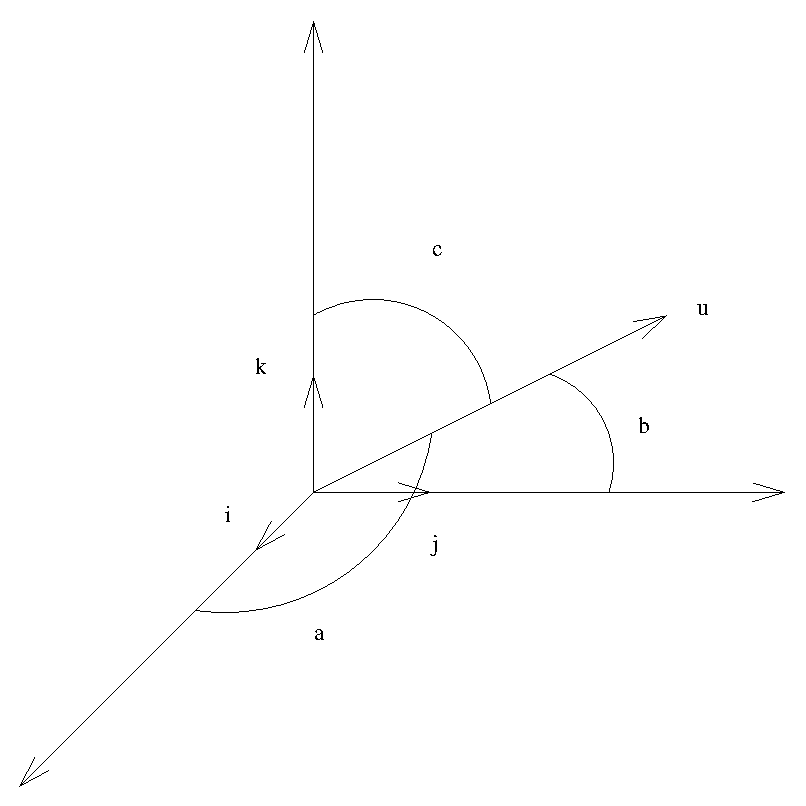
\includegraphics[height=2in]{../../modules/vectors/pictures/ok-direction_angles.eps}
\end{figure}


$\textbf{u} = \langle u_1, u_2, u_3\rangle, \qquad \alpha = \angle (\textbf{u},\textbf{i}) \qquad \beta =
\angle (\textbf{u},\textbf{j}) \qquad \gamma = \angle (\textbf{u},\textbf{k}) \; .$

$$\cos{\alpha} = \frac{\textbf{u} \cdot \textbf{i}}{|\textbf{u}|\, |\textbf{i}|} =
\frac{u_1}{\sqrt{u_1^2+u_2^2+u_3^2}}$$

Similar for $\cos{\beta}$ and $\cos{\gamma}$. Then:
%
$$\cos^2\alpha + \cos^2\beta + \cos^2\gamma = 1\; .$$

\end{frame}

%\begin{frame}
 \frametitle{Rotational Effect}

 \begin{itemize}
  \item Rigid rod $OP$, fixed at $O$, $\textbf{r}=\textbf{OP}$. Force $\textbf{F}$ applied at $P$.
 \end{itemize}
%
\begin{figure}[h]
  \psfrag{F}{$\textbf{F}$}
  \psfrag{r}{$\textbf{r}$}
  \psfrag{O}{$O$}
  \psfrag{P}{$P$}
  \psfrag{}{$\alpha$}
  \psfrag{pfr}{$\textbf{proj}_{\bm{r}} \textbf{F}$}
  \psfrag{ofr}{$\textbf{orth}_{\bm{r}} \textbf{F}$}
  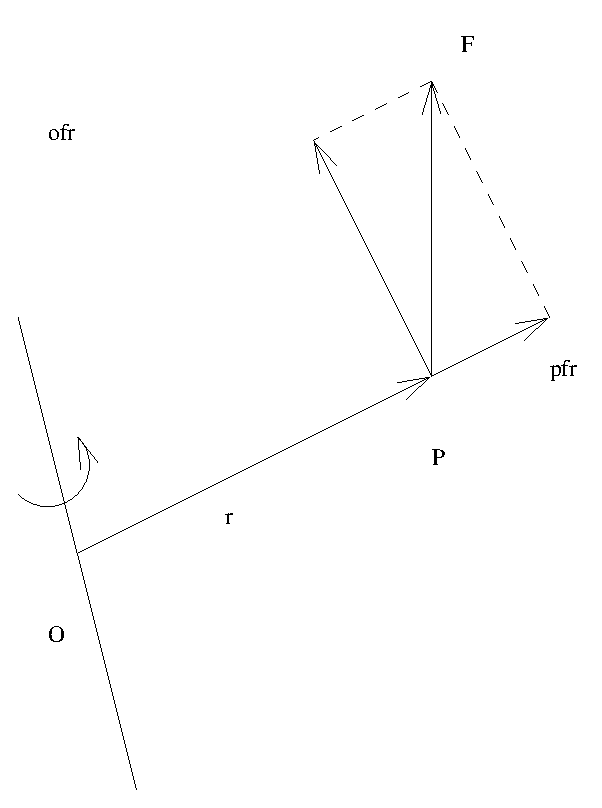
\includegraphics[height=1.5in]{../../modules/vectors/pictures/ok-torque.eps}
\end{figure}
%
\pause
\begin{itemize}
  \item $\textbf{proj}_{\bm{r}} \textbf{F}$: \pause no effect;
  \item $\textbf{orth}_{\bm{r}} \textbf{F}$: \pause rotational effect:\pause
  \begin{itemize}
    \item Axis of rotation: \pause perpendicular to $\textbf{r}$ and $\textbf{F}$;\pause
    \item Angular velocity: \pause proportional to $|\textbf{orth}_{\bm{r}} \textbf{F}|$;\pause
    \item Linear velocity: \pause proportional to $|\textbf{r}| \, |\textbf{orth}_{\bm{r}} \textbf{F}|$.
  \end{itemize}
\end{itemize}

\end{frame}
%\begin{frame}
\frametitle{Torque}

Rotation in space $\Longleftrightarrow$ vector\pause
  \begin{itemize}
   \item Axis of rotation $\Longleftrightarrow$ Support of direction \pause
   \item Sense of rotation  $\Longleftrightarrow$ Direction of vector \pause
  \begin{itemize}
      \item Convention: Right Hand Rule\pause
  \end{itemize}
  \item Angular velocity $\Longleftrightarrow$ (proportional to) Magnitude of vector\pause
  \end{itemize}
\begin{center}
 $(\textbf{r}, \textbf{F}) \rightarrow$ rotation $\rightarrow$ vector = torque, $\bm{\tau}$
\end{center}



\begin{itemize}
 \item Support of direction: perpendicular to $\textbf{r}$ and $\textbf{F}$;
 \item Direction: Right Hand Rule;
 \item Magnitude: $|\bm{\tau}| = |\textbf{r}| \, |\textbf{orth}_{\bm{r}} \textbf{F}|$
\end{itemize}

\end{frame}
%\begin{frame}
\frametitle{The Cross Product $\times$}
\begin{columns}
\column{0.35\textwidth}
\psset{xunit=2cm, yunit=2cm}
\begin{pspicture}(-0.2,-0.2)(1.2,1.2)
\tiny
\renewcommand{\fcScreenStyle}{[0 0.1 1]}%
\only<5->{\renewcommand{\fcScreen}{[-1 1 -0.5] 0}}%
\only<6->{\renewcommand{\fcScreen}{[-0.8 0.8 -0.5] 0}}%
\only<7->{\renewcommand{\fcScreen}{[-0.6 0.6 -0.5] 0}}%
\only<8->{\renewcommand{\fcScreen}{[-0.4 0.4 -0.5] 0}}%
\only<9->{\renewcommand{\fcScreen}{[-0.2 0.2 -0.5] 0}}%
\only<10->{\renewcommand{\fcScreen}{[-0.1 0.1 -0.5] 0}}%
\only<11->{\renewcommand{\fcScreen}{[-0.05 0.05 -0.5] 0}}%
\fcLineIIId[arrows=->]{[0 0 0]}{[1 0 0]}
\fcLineIIId[arrows=->]{[0 0 0]}{[1 1 0]}
\fcLineIIId[arrows=->]{[0 0 0]}{[0 0 1]}
\fcPutIIId[r]{[0 0 1]}{$\fcv u \times \fcv v$}
\fcAngleIIId[arrows=->, linecolor=blue]{[1 0 0]}{[1 1 0]}{0.4}
\fcPutIIId[lt]{[0.4 0.2 0]}{$\alpha$}
\fcPutIIId[t]{[1 0 -0.1]}{$\fcv u$}
\fcPutIIId[t]{[1 1 -0.1]}{$\fcv v$}
\uncover<3->{%
\fcLineIIId[arrows=->]{[0 0 0]}{[0 1 0]}
\fcPutIIId[rb]{[0 1 0]}{$\textbf{orth}_{\fcv u} \fcv v$}%
\fcPerpendicularIIId[linestyle=dashed]{[1 1 0]}{[0 1 0]}{0.2}%
}%
\only<2>{\fcPerpendicularIIId{[0 0 1]}{[-1 -1 0]}{0.2}%
\fcPerpendicularIIId{[0 0 1]}{[-1 0 0]}{0.2}%
}%
\end{pspicture}
\column{0.65\textwidth}

\begin{definition}[Cross product]
$\fcv{u} \times \fcv{v}$ is the vector uniquely determined by the following.
\begin{itemize}
\item If $\fcv{u}$, $\fcv{v}$ are non-zero and non-collinear.
\begin{itemize}
\item \alert<2>{ $\fcv{u} \times \fcv{v}$ is perpendicular to both $\fcv{u}$ and $\textbf{v}$.}
\item The magnitude of $\fcv{u} \times \fcv{v}$ equals $|\fcv{u}| \alert<3>{| \textbf{orth}_{\fcv u} \fcv v |}=|\textbf{u}| \alert<3>{|\textbf{v}| \sin{\alpha}}$.
\item \alert<4-12>{The direction of $\textbf{u} \times \textbf{v}$ is such that when viewed from the tip of $\fcv{u}\times \fcv v$, $\fcv v$ is counter-clockwise from $\fcv u$.}
\end{itemize}
\item If $\fcv{u}$, $\fcv{v}$ are colinear or zero then $\fcv u \times \fcv v=\fcv 0$.
\end{itemize}
\end{definition}
\end{columns}
\uncover<12->{\alert<12>{There are a couple of hand rules to help figure out the direction of the cross product.}}
\end{frame}
%\begin{frame}
 \frametitle{Properties of Cross Product}
Let $\textbf{u}$, $\textbf{v}$ non-zero vectors, $\alpha = \angle(\textbf{u},\textbf{v})$.


\begin{itemize}
\item<2-> $|\textbf{v} \times \textbf{u}|  = | \textbf{u} \times \textbf{v}|$.

\uncover<3->{Indeed, that is because $$|\textbf{orth}_{\bm{u}} \textbf{v}| = |\textbf{v}|\sin\alpha
\Longrightarrow |\textbf{u} \times \textbf{v}| = |\textbf{u}| \, |\textbf{v}| \, \sin{\alpha}$$
}

 \item<4-> Cross product is anti-symmetric:
$$\textbf{v} \times \textbf{u} = - \textbf{u} \times \textbf{v} \; .$$
\item<5-> Cross product is linear in each argument:
%
$$ \textbf{u} \times (a\textbf{v} + b\textbf{w}) =
a \textbf{u} \times \textbf{v} + b \textbf{u} \times \textbf{w}$$
%
$$(a\textbf{u} + b\textbf{w}) \times \textbf{v} =
a \textbf{u} \times \textbf{v} + b \textbf{w} \times \textbf{v}$$
\end{itemize}

\end{frame}
%\begin{frame}
 \frametitle{Cross Product in Coordinates}

\begin{itemize}
\item Let $\fcv{i}$, $\fcv{j}$, $\fcv{k}$: unit vectors along coordinate axes.
\item We have that
\[ 
\begin{array}{r@{}c@{}cr@{}c@{}cr@{}c@{}c}
\fcv{i} \times \fcv{i} &~=~& \fcv{0}, & \fcv{j} \times \fcv{j} &~=~&\fcv{0} , & \fcv{k} \times \fcv{k} &~=~& \fcv{0} \\
\fcv{i} \times \fcv{j} &~=~& \fcv{k}, & \fcv{j} \times \fcv{k} &~=~& \fcv{i}, &  \fcv{k} \times \fcv{i}& ~=~& \fcv{j}\\
\fcv{j} \times \fcv{i} &~=~& -\fcv{k}, & \fcv{k} \times \fcv{j} &~=~& -\fcv{i},& \fcv{i} \times \fcv{k} &~=~& -\fcv{j}
\end{array}
\]
\item Let $\begin{array}{rclcl}
\fcv{u} &=& u_1 \fcv{i} + u_2 \fcv{j} + u_3 \fcv{k} &=& \langle u_1, u_2, u_3 \rangle \\
\fcv{v}&=&v_1 \fcv{i} + v_2 \fcv{j} + v_3 \fcv{k} &=& \langle v_1, v_2, v_3 \rangle\end{array}$.
\item 
\[\begin{array}{rcl}
\fcv{u} \times \fcv{v} &=& (u_1 \fcv{i} + u_2 \fcv{j} + u_3 \fcv{k})
\times (v_1 \fcv{i} + v_2 \fcv{j} + v_3 \fcv{k})\\
&=& (u_2v_3 -u_3v_2) \fcv{i} + (u_3v_1-u_1v_3) \fcv{j} + (u_1v_2-u_2v_1) \fcv{k} \\
\fcv{u} \times \fcv{v} &=& 
\langle u_1, u_2, u_3 \rangle \times \langle v_1, v_2, v_3 \rangle =
\left|
\begin{array}{ccc}
\fcv{i} & \fcv{j} & \fcv{k} \\
u_1 & u_2 & u_3 \\
v_1 & v_2 & v_3
\end{array}
\right|
\end{array}
\]



\end{itemize}
\end{frame}
%\begin{frame}
$\displaystyle
\fcv{u} \times \fcv{v} = ( u_1, u_2, u_3 ) \times ( v_1, v_2, v_3 ) =
\left|  \begin{array}{ccc}
\fcv{i} & \fcv{j} & \fcv{k} \\
u_1 & u_2 & u_3 \\
v_1 & v_2 & v_3
\end{array}\right|
$
\begin{example}
\begin{columns}[c]
\column{0.3\textwidth}
\column{0.7\textwidth}
Find $\fcv u \times \fcv v$, where $\fcv{u} = ( 1,2,3)$ and $\fcv{v} = ( 6,5,4 )$.
\end{columns}

\[
\begin{array}{rcl}
\uncover<2->{%
\fcv{u} \times \fcv{v} &=& ( 1, 2, 3 ) \times ( 6, 5, 4 ) =
\left|
\begin{array}{ccc}
\fcv{i} & \fcv{j} & \fcv{k} \\
1 & 2 & 3 \\
6 & 5 & 4
\end{array}
\right| \\
} %uncover
\uncover<3->{%
&=&
\left|\begin{array}{cc}
2 & 3\\
5 & 4
\end{array}\right|\fcv{i} -
\left| \begin{array}{cc}
1 & 3\\
6 & 4
\end{array}\right| \fcv{j} +
\left| \begin{array}{cc}
1 & 2\\
6 & 5
\end{array}\right| \fcv{k}  \\~\\
} %uncover
\uncover<4->{%
&=&(2\cdot 4 -3\cdot 5) \fcv{i} - (1\cdot 4 - 3\cdot 6) \fcv{j} + (1 \cdot 5 - 2\cdot 6) \fcv{k} \\~\\
}%uncover
\uncover<5->{%
&=& -7 \fcv{i} + 14 \fcv{j} -7 \fcv{k} =( -7, 14, -7)\; .
}
\end{array}
\]
%
\end{example}
\end{frame}

%\begin{frame}
\frametitle{Use $\times$ to find vector perpendicular to two given}
Recall $\textbf{u} \times \textbf{v}$ is perpendicular to $\textbf{u}$ and $\textbf{v}$.
\begin{example}
Find a vector perpendicular to $\textbf{u} =\langle1,1,0\rangle = \textbf{i}+\textbf{j}$ and $\textbf{v}=\textbf{j}+\textbf{k}=\langle 0,1,1 \rangle$:

\[
\begin{array}{rcl}
 \textbf{w} &= & (\textbf{i}+\textbf{j}) \times (\textbf{j}+\textbf{k}) =
\textbf{i} \times \textbf{j} + \textbf{i} \times \textbf{k} +
\textbf{j} \times \textbf{j} + \textbf{j} \times \textbf{k} = \\
& = & \textbf{k} -\textbf{j}+\textbf{0}+\textbf{i} = \textbf{i} - \textbf{j} + \textbf{k} = \langle1,-1,1\rangle\; .
\end{array}
\]
\end{example}
\end{frame}

\begin{frame}
\frametitle{Use $\times$ to find area of triangle in space}
\begin{columns}
\column{0.3\textwidth}
\psset{xunit=2cm, yunit=2cm}
\begin{pspicture}(-0.3,-0.1)(1.4,1.4)%
\psline[arrows=->](0,0)(1.2,0)%
\psline[arrows=->](0,0)(0.2,1)%
\psline[arrows=->](1.2,0)(0.2,1)%
\psline(0.2,1)(1.4,1)(1.2,0)%
\rput[t](0,-0.1){$A$}
\rput[tl](1.2,-0.1){$B$}
\rput[bl](1.4,1.1){$D$}
\rput[br](0.2,1.1){$C$}
\uncover<2->{%
\rput[l](0.25,0.5){$\fcv w$}%
\fcPerpendicular{[0.2 1]}{[1 0]}{0.1}%
\psline[arrows=->](0.2,0 )(0.2,1)%
}%
\rput[t](0.5, -0.1){$\fcv u$}
\rput[r](0,0.5){$\fcv v$}
\end{pspicture}  
\column{0.7\textwidth}
\begin{itemize}
\item $A$, $B$, $C$ points in space, $\textbf{u} = \textbf{AB}$, $\textbf{v}=\textbf{AC}$. 
\item<2-> Then $|\textbf{w}| = |\textbf{orth}_{\bm{u}} \textbf{v}| = \text{ distance from } C \text{ to } AB\; .$
\item<3-> $|\textbf{u} \times \textbf{v}| = |\textbf{orth}_{\bm{u}} \textbf{v}| \, |\textbf{u}| =
2 \text{area}(ABC) = \text{area}(ABDC)$
\item<4-> $|\textbf{u} \times \textbf{v}|$ = Area of parallelogram on sides $\textbf{u}$ and $\textbf{v}$.
\end{itemize}
%
\end{columns}
\end{frame}

\begin{frame}
\begin{example}
\begin{columns}
\column{0.3\textwidth}
\psset{xunit=0.7cm, yunit=0.7cm}
\begin{pspicture}(-0.1, -1)(4,3.5)
\fcBoundingBox{-0.2}{-1}{4}{3.5}
\fcAxesIIId{3}{3}{3}%
\pscustom*[linecolor=cyan]{%
\fcPolyLineIIId{[1 2 3] [2 3 1] [3 1 2] [1 2 3]}
}
\end{pspicture}
\column{0.7\textwidth}

Find the area of the triangle $A(1,2,3)$, $B(2,3,1)$, $C(3,1,2)$.

\end{columns}
\[\begin{array}{rcl}
\displaystyle \text{Area}(ABC) &=&\displaystyle \frac{1}{2}|\textbf{AB} \times \textbf{AC}| =
\frac{1}{2}|\langle 1,1,-2\rangle \times \langle 2, -1, -1\rangle | \\~\\
&=&\displaystyle\frac{1}{2} |\langle -3, -3, -3 \rangle| \\~\\
&=&\displaystyle \frac{3\sqrt{3}}{2}\; .
\end{array}
\]

\end{example}
\end{frame}
%\begin{frame}[label=current]
\frametitle{Scalar Triple Product}
\begin{columns}
\column{0.25\textwidth}
  \psfrag{u}{$\textbf{u}$}
  \psfrag{v}{$\textbf{v}$}
  \psfrag{w}{$\textbf{w}$}
  \psfrag{uxv}{$\textbf{u}\times \textbf{v}$}
  \psfrag{ow}{$\textbf{r}$}
  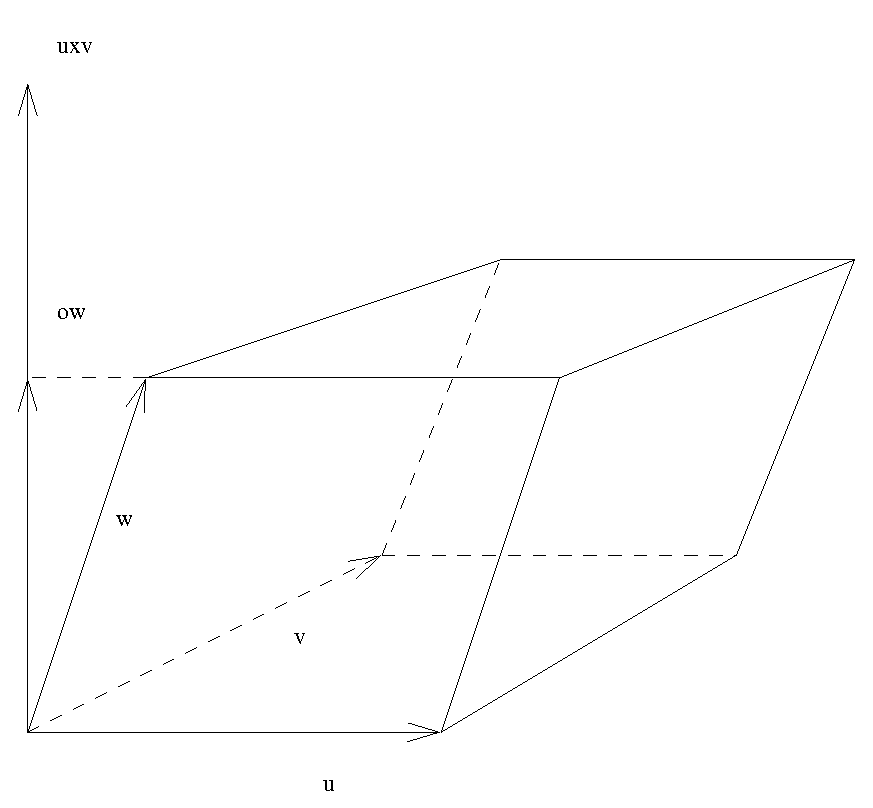
\includegraphics[height=1in]{../../modules/vectors/pictures/ok-volume_box.eps}

\column{0.75\textwidth}
\begin{itemize}
\item $A$, $B$, $C$, $D$ points in space;
\item<2-> $\textbf{u} = \textbf{AB}$, $\textbf{v}=\textbf{AC}$, $\textbf{w}=\textbf{AD}$;
\item<3-> $R=R(\textbf{u},\textbf{v},\textbf{w})$: box on sides $\textbf{u}$, $\textbf{v}$, $\textbf{w}$.\pause
\item<4-> $\text{Vol}(R) = |\textbf{u} \times \textbf{v}| |\textbf{r}| = |\textbf{u} \times \textbf{v}| \, |\textbf{proj}_{\bm{u} \times \bm{v}} \textbf{w}| =
|\textbf{w} \cdot (\textbf{u} \times \textbf{v})|\; .$
\end{itemize}
\end{columns}
\uncover<5->{
\begin{definition}
The quantity $\textbf{w} \cdot (\textbf{u} \times \textbf{v})$ is called the scalar triple product of $\fcv w, \fcv u, \fcv v$.
\end{definition}
}
\uncover<6->{
\begin{itemize}
\item If $\textbf{u} =\langle u_1,u_2,u_3\rangle$,
$\textbf{v} =\langle v_1,v_2,v_3\rangle$, and $\textbf{w} =\langle w_1,w_2,w_3\rangle$, then
%
$$\textbf{w} \cdot (\textbf{u} \times \textbf{v}) = \left|
\begin{array}{ccc}
w_1 & w_2 & w_3 \\
u_1 & u_2 & u_3 \\
v_1 & v_2 & v_3
\end{array}
 \right|$$
\end{itemize}
}
\end{frame}
%\begin{frame}
  \frametitle{Orientations of Space}

\begin{itemize}
 \item The following are equivalent:
\begin{itemize}
  \item Every vector in space can be decomposed along $\textbf{u}$, $\textbf{v}$, $\textbf{w}$;
  \item The box $R(\textbf{u},\textbf{v},\textbf{w})$ is non-degenerate;
  \item $Vol(R(\textbf{u},\textbf{v},\textbf{w})) \neq 0$;
  \item $\textbf{u} \cdot (\textbf{v} \times \textbf{w}) \neq 0$.
\end{itemize}
%
\item \pause If any of the above is valid: $\{ \textbf{u}, \textbf{v}, \textbf{w}\}$ is a frame.

\item Rectangular coordinate system $\to$ fundamental frame $\{ \textbf{u}, \textbf{v}, \textbf{w}\}$

\item Consistent Right Hand Rule ($\textbf{w}=\textbf{u} \times \textbf{v}$) if and only if
%
$$\textbf{u} \cdot (\textbf{v} \times \textbf{w}) >0$$
%
The frame $\{ \textbf{u}, \textbf{v}, \textbf{w}\}$ is positively oriented if
$\textbf{u} \cdot (\textbf{v} \times \textbf{w}) >0$
%
\end{itemize}

\end{frame}


%%\begin{comment}
\begin{frame}
\frametitle{Rectangular/Cartesian Coordinates}
\begin{columns}
\column[t]{0.3\textwidth}
\psset{xunit=0.7cm, yunit=0.7cm}
\begin{pspicture}(-0.5 ,-2)(4.5, 4)
\fcBoundingBox{-0.5}{-2}{4.5}{4}
\tiny
\uncover<3->{
\fcLineIIId{[0 0 0]}{[3 0 0]}
\fcLineIIId{[0 0 0]}{[0 3 0]}
\fcLineIIId{[0 0 0]}{[0 0 3]}
}
\uncover<4->{
\fcLineIIId[arrows=->]{[0 0 0]}{[3 0 0]}
\fcLineIIId[arrows=->]{[0 0 0]}{[0 3 0]}
\fcLineIIId[arrows=->]{[0 0 0]}{[0 0 3]}
}
\uncover<5->{
\fcPutIIId[t]{[3 0 0]}{\alertNoH{5}{$x$}}
\fcPutIIId[lb]{[0 3 0]}{\alertNoH{5}{$y$}}
\fcPutIIId[b]{[0 0 3]}{\alertNoH{5}{$z$}}
}
\uncover<2->{ %
\fcPutIIId[r]{[0 0 0]}{$O~~~$} %
\fcDotIIId[linecolor=black]{[0 0 0]} %
}
\end{pspicture}


\vfill
\column{0.7\textwidth}
\begin{itemize}
\item<1-> A Cartesian coordinate system is given by fixing:
\begin{itemize}
\item<2-> a point $O$ (called the origin),
\item<3-> 3 pairwise perpendicular lines intersecting at the origin,
\item<4-> a direction in each of the coordinate axis.
\end{itemize}
\item<5-> The three lines are labeled as $x$-axis, $y$-axis and $z$-axis.
\end{itemize}

\vskip 3cm
\end{columns}


%
\end{frame}

\begin{frame}
\frametitle{Rectangular/Cartesian Coordinates}
\begin{columns}
\column[t]{0.3\textwidth}
\psset{xunit=0.7cm, yunit=0.7cm}
\begin{pspicture}(-0.5 ,-2)(4.5, 4)
\fcBoundingBox{-0.5}{-2}{4.5}{4}
\tiny
\renewcommand{\fcScreen}{[-1 1.1 -0.5] 0}
\fcAxesIIId{3}{3}{3}
\fcPutIIId[r]{[0 0 0]}{$O~$}
\fcPutIIId[b]{[2.5 2.5 2.8]}{$P(x_P,y_P,z_P)$}
\uncover<9->{
\fcLineIIId[linecolor=gray]{[2.5 2.5 2.5]}{[2.5 2.5 0]}
\fcLineIIId[linecolor=gray]{[2.5 2.5 2.5]}{[2.5 0 2.5]}
\fcLineIIId[linecolor=gray]{[2.5 2.5 2.5]}{[0 2.5 2.5]}
\fcLineIIId[linecolor=gray]{[0 2.5 2.5]}{[0 0 2.5]}
\fcLineIIId[linestyle=dashed, linecolor=gray]{[0 2.5 2.5]}{[0 2.5 0]}
\fcLineIIId[linecolor=gray]{[2.5 0 2.5]}{[0 0 2.5]}
\fcLineIIId[linecolor=gray]{[2.5 0 2.5]}{[2.5 0 0]}
\fcLineIIId[linestyle=dashed, linecolor=gray]{[2.5 2.5 0]}{[0 2.5 0]}
\fcLineIIId[linecolor=gray]{[2.5 2.5 0]}{[2.5 0 0]}%
}%
\fcDotIIId{[2.5 2.5 2.5]}%
\uncover<3-8>{%
\fcPerpendicularIIId{[2.5 2.5 2.5]}{[1 0 0]}{0.3}%
\fcPutIIId[t]{[2.5 0 -0.1]}{$Q$}%
}%
\uncover<4->{\fcPutIIId[t]{[1.25 0 -0.1]}{$x_P$}}%
\uncover<6-8>{%
\fcPerpendicularIIId{[2.5 2.5 2.5]}{[0 1 0]}{0.3}%
\fcPerpendicularIIId{[2.5 2.5 2.5]}{[0 0 1]}{0.3}%
}%
\uncover<6->{%
\fcPutIIId[b]{[0 1.25 0.1]}{$y_P$}%
\fcPutIIId[r]{[0 0 1.25]}{$z_P~~$}%
}
\end{pspicture}


\vfill
\column{0.7\textwidth}
\begin{itemize}
\item<1-> $P$ -point. We assign to it triple $(x_P,y_P,z_P)$.
\item<2-> Assignment will be such that distinct points are assigned distinct triples.
\item<3-> $Q=$ base of perpendicular from $P$ to $x$-axis.
\item<4-> Define $x_P$ as \alertNoH{5}{signed distance b-n $O$ and $Q$}.
\item<5-> Take distance with \alertNoH{5}{$+$ sign if $OQ$ points in direction of $x$-axis, $-$ sign else}.
\item<6-> Definitions of $y_P$, $z_P$ are similar.
\item<7-> $(x_P,y_P,z_P)$ = Cartesian coordinates of $P$. 
\item<8-> $x_P$ is called the $x$-coordinate of $P$,  and so on for other axes.
\item<9-> $(x_P, y_P, z_P)$ = singed lengths of edges of the rectangular box indicated in the picture.
\end{itemize}

\vfill
\end{columns}

\vskip 5cm

\end{frame}
%\end{comment}
%\begin{frame}
 \frametitle{Polar curvilinear ``boxes''}

 Polar ``wedge'':
 %
$$C  = \{ P(r,\theta) \; | \;r_0 \leqslant
r \leqslant r_0+\Delta r,  \theta_0 \leqslant \theta
\leqslant \theta_0+\Delta \theta\} \; .$$
%
Shape? \pause Area = ...?

\end{frame}
%\begin{frame}
\frametitle{Spherical curvilinear ``boxes''}


\begin{columns}[T]
\column{0.4\textwidth}

\psset{xunit=1.5cm, yunit=1.5cm}
\begin{pspicture}(-0.6, -0.85)(2.4,1.85)
\tiny
\renewcommand{\fcScreen}{[-5 1 -2.4] 0}
\pstVerb{10 dict begin%
/rhoMin 1 def%
/rhoMax 2 def%
/thetaMin 20 def%
/thetaMax 70 def%
/phiMin 20 def%
/phiMax 70 def%
/xSph {theta cos phi sin rho mul mul} def%
/ySph {theta sin phi sin rho mul mul} def%
/zSph {phi cos rho mul} def%
}%
\fcAxesIIId{2}{2}{2}
\uncover<10->{
\pscustom*[linecolor=pink]{%
\fcCurveIIId{phiMin}{phiMax}{[3 dict begin /rho rhoMin def /phi t def /theta thetaMin def xSph ySph zSph end]}
\fcCurveIIId{rhoMin}{rhoMax}{[3 dict begin /rho t def /phi phiMax def /theta thetaMin def xSph ySph zSph end]}
\fcCurveIIId{thetaMin}{thetaMax}{[3 dict begin /rho rhoMax def /phi phiMax def /theta t def xSph ySph zSph end]}
\fcCurveIIId{phiMax}{phiMin}{[3 dict begin /rho rhoMax def /phi t def /theta thetaMax def xSph ySph zSph end]}
\fcCurveIIId{thetaMax}{thetaMin}{[3 dict begin /rho rhoMax def /phi phiMin def /theta t def xSph ySph zSph end]}
\fcCurveIIId{rhoMax}{rhoMin}{[3 dict begin /rho t def /phi phiMin def /theta thetaMin def xSph ySph zSph end]}
}%
}%
\fcLineIIId[linestyle=dashed]{[0 0 0]}{[0 2 0]}

\uncover<7->{\fcCurveIIId{rhoMin}{rhoMax}{[3 dict begin /rho t def /phi phiMin def /theta thetaMin def xSph ySph zSph end]}}
\uncover<5->{\fcCurveIIId{rhoMin}{rhoMax}{[3 dict begin /rho t def /phi phiMax def /theta thetaMin def xSph ySph zSph end]}}
\uncover<9->{\fcCurveIIId[linestyle=dashed, linecolor=red]{rhoMin}{rhoMax}{[3 dict begin /rho t def /phi phiMin def /theta thetaMax def xSph ySph zSph end]}}
\uncover<9->{\fcCurveIIId[linestyle=dashed, linecolor=red]{rhoMin}{rhoMax}{[3 dict begin /rho t def /phi phiMax def /theta thetaMax def xSph ySph zSph end]}}

\uncover<8->{%
\fcCurveIIId[linestyle=dashed, dash = 2.6pt,  linecolor=red] {thetaMin}{thetaMax}{[3 dict begin /rho rhoMin def /phi phiMin def /theta t def xSph ySph zSph end]}
\fcCurveIIId{thetaMin}{thetaMax}{[3 dict begin /rho rhoMax def /phi phiMin def /theta t def xSph ySph zSph end]}
\fcCurveIIId[linestyle=dashed, linecolor=red]{thetaMin}{thetaMax}{[3 dict begin /rho rhoMin def /phi phiMax def /theta t def xSph ySph zSph end]}
\fcCurveIIId{thetaMin}{thetaMax}{[3 dict begin /rho rhoMax def /phi phiMax def /theta t def xSph ySph zSph end]}
}%

\uncover<4->{\fcCurveIIId{phiMin}{phiMax}{[3 dict begin /rho rhoMin def /phi t def /theta thetaMin def xSph ySph zSph end]}}
\uncover<9->{\fcCurveIIId[linestyle=dashed, linecolor=red]{phiMin}{phiMax}{[3 dict begin /rho rhoMin def /phi t def /theta thetaMax def xSph ySph zSph end]}}
\uncover<6->{\fcCurveIIId{phiMin}{phiMax}{[3 dict begin /rho rhoMax def /phi t def /theta thetaMin def xSph ySph zSph end]}}
\uncover<9->{\fcCurveIIId{phiMin}{phiMax}{[3 dict begin /rho rhoMax def /phi t def /theta thetaMax def xSph ySph zSph end]}}
\pstVerb{end}
\end{pspicture}

\psset{xunit=1cm, yunit=1cm}
\begin{pspicture}(-0.6, -2)(3,2.4)
\tiny
\pstVerb{10 dict begin%
/rhoMin 1 def%
/rhoMax 2 def%
/thetaMin 20 57.2957795 div def%
/thetaMax 70 57.2957795 div  def%
/phiMin 20 57.2957795 div def%
/phiMax 70 57.2957795 div def%
}%
\fcAxesIIId[arrows=->, xLabel=$~~\rho$, yLabel=$~~\phi$, zLabel=$~~\theta$]{2.5}{3.8}{2.5}
\pscustom*[linecolor=cyan]{%
\fcPolyLineIIId{[rhoMin phiMin thetaMin] [rhoMax phiMin thetaMin] [rhoMax phiMax thetaMin] [rhoMax phiMax thetaMax] [rhoMin phiMax thetaMax] [rhoMin phiMin thetaMax] [rhoMin phiMin thetaMin]}
}
\fcLineIIId[linestyle=dashed]{[0 0 0]}{[0 3.8 0]}
\fcDotIIId{[rhoMin 0 0 ]}
\fcPutIIId[t]{[rhoMin 0 -0.2 ]}{$\rho_{min}$}
\fcDotIIId{[rhoMax 0 0 ]}
\fcPutIIId[t]{[rhoMax 0 -0.2 ]}{$\rho_{max}$}
\fcDotIIId{[0 0 thetaMin  ]}
\fcPutIIId[r]{[0 0 thetaMin]}{$\theta_{min}~~$}
\fcDotIIId{[0 0 thetaMax]}
\fcPutIIId[r]{[0 0 thetaMax]}{$\theta_{max}~~$}
\fcDotIIId{[0  phiMin 0  ]}
\fcPutIIId[b]{[0 phiMin 0.2 ]}{$~\phi_{min}$}
\fcDotIIId{[0  phiMax 0  ]}
\fcPutIIId[b]{[0 phiMax 0.2 ]}{$\phi_{max}$}

\fcLineIIId[linecolor=blue, linestyle=dashed]{[rhoMin phiMax thetaMin]}{[rhoMax phiMax thetaMin]}
\uncover<5-9>{\fcLineIIId[linecolor=red, linewidth=2pt, linestyle=dashed]{[rhoMin phiMax thetaMin]}{[rhoMax phiMax thetaMin]}}
\fcLineIIId[linecolor=blue]{[rhoMax phiMax thetaMin]}{[rhoMax phiMin thetaMin]}
\uncover<6-9>{\fcLineIIId[linecolor=red, linewidth=2pt]{[rhoMax phiMax thetaMin]}{[rhoMax phiMin thetaMin]}
}
\fcLineIIId[linecolor=blue]{[rhoMax phiMin thetaMin]}{[rhoMin phiMin thetaMin]}
\uncover<7-9>{\fcLineIIId[linecolor=red, linewidth=2pt]{[rhoMax phiMin thetaMin]}{[rhoMin phiMin thetaMin]}}
\fcLineIIId[linecolor=blue, linestyle=dashed]{[rhoMin phiMin thetaMin]}{[rhoMin phiMax thetaMin]}
\uncover<4-9>{\fcLineIIId[linecolor=red, linewidth=2pt, linestyle=dashed]{[rhoMin phiMin thetaMin]}{[rhoMin phiMax thetaMin]}}

\fcLineIIId[linecolor=blue, linestyle=dashed]{[rhoMin phiMax thetaMax]}{[rhoMin phiMax thetaMin]}
\fcLineIIId[linecolor=blue]{[rhoMax phiMax thetaMax]}{[rhoMax phiMax thetaMin]}
\fcLineIIId[linecolor=blue]{[rhoMax phiMin thetaMax]}{[rhoMax phiMin thetaMin]}
\fcLineIIId[linecolor=blue]{[rhoMin phiMin thetaMax]}{[rhoMin phiMin thetaMin]}
\uncover<8-9>{%
\fcLineIIId[linecolor=red, linestyle=dashed, linewidth=2pt]{[rhoMin phiMax thetaMax]}{[rhoMin phiMax thetaMin]}
\fcLineIIId[linecolor=red, linewidth=2pt]{[rhoMax phiMax thetaMax]}{[rhoMax phiMax thetaMin]}
\fcLineIIId[linecolor=red, linewidth=2pt]{[rhoMax phiMin thetaMax]}{[rhoMax phiMin thetaMin]}
\fcLineIIId[linecolor=red, linewidth=2pt]{[rhoMin phiMin thetaMax]}{[rhoMin phiMin thetaMin]}
}%
\fcLineIIId[linecolor=blue]{[rhoMin phiMax thetaMax]}{[rhoMax phiMax thetaMax]}
\fcLineIIId[linecolor=blue]{[rhoMax phiMax thetaMax]}{[rhoMax phiMin thetaMax]}
\fcLineIIId[linecolor=blue]{[rhoMax phiMin thetaMax]}{[rhoMin phiMin thetaMax]}
\fcLineIIId[linecolor=blue]{[rhoMin phiMin thetaMax]}{[rhoMin phiMax thetaMax]}
\uncover<9>{%
\fcLineIIId[linecolor=red, linewidth=2pt]{[rhoMin phiMax thetaMax]}{[rhoMax phiMax thetaMax]}
\fcLineIIId[linecolor=red, linewidth=2pt]{[rhoMax phiMax thetaMax]}{[rhoMax phiMin thetaMax]}
\fcLineIIId[linecolor=red, linewidth=2pt]{[rhoMax phiMin thetaMax]}{[rhoMin phiMin thetaMax]}
\fcLineIIId[linecolor=red, linewidth=2pt]{[rhoMin phiMin thetaMax]}{[rhoMin phiMax thetaMax]}
}%
\pstVerb{end}
\end{pspicture}

\column{0.6\textwidth}
\begin{itemize}
\item Cut off a rectangular box $B$ in the $\rho, \phi, \theta$-coordinates.
$
B:=\left\{(\rho, \phi, \theta) |\left| \begin{array}{ccccc}
\rho_{min} &\leq& \rho &\leq& \rho_{max} \\
\phi_{min} &\leq& \phi &\leq& \phi_{max}\\
\theta_{min} &\leq& \theta &\leq& \theta_{max}\\
\end{array}\right.\right\}
$
\item<2-> As $(\rho, \phi, \theta)$ traverse $B$, the point $P(\rho, \phi,\theta)$ traverses curvilinear ``box'' $Y$: %in the $x,y,z$-coordinates:
\[
Y = \left\{ P(\rho, \phi, \theta) | (\rho, \phi, \theta)\in B \right\}.
\]
\item<3-> \alertNoH{3-10}{ What is the shape of that curvilinear box?}
\item<11-> What is the volume?
\end{itemize}
\end{columns}
\end{frame}


%\begin{frame}
\frametitle{Transition Spherical - Rectangular coordinates}
\begin{columns}
\column{0.4\textwidth}
\psset{xunit=1cm, yunit=1cm}
\begin{pspicture}(-3,-2)(2,2)
\tiny
\renewcommand{\fcScreen}{[-1 -0.4 -0.25] -1}
\fcLineIIId[arrows=->]{[0 0 0]}{[5 0 0 ]}
\fcLineIIId[arrows=->]{[0 0 0]}{[0 5 0 ]}
\fcLineIIId[arrows=->]{[0 0 0]}{[0 0 5 ]}
\fcPutIIId[r]{[0 -0.15 0.15]}{\alert<2,3,4>{$O$}}
\fcLineIIId[linecolor=gray]{[3 0 0]}{[3 3 0]}
\fcLineIIId[linecolor=gray]{[3 3 0]}{[0 3 0]}
\fcLineIIId{[0 0 0]}{[3 3 0]}
\fcLineIIId{[3 3 0]}{[3 3 3]}
\fcLineIIId{[0 0 0]}{[3 3 3]}
\fcLineIIId{[0 0 3]}{[3 3 3]}
\fcPutIIId[l]{[3.1 3.1 3.1]}{\alert<4>{$P$}}
\fcPutIIId[r]{[1.5 -0.1 0]}{$\alert<1>{x}$}
\fcPutIIId[t]{[3.1 3.1 0]}{\alert<2,3>{$Q$}}
\uncover<2->{\fcPutIIId[l]{[1.4 1.5 0]}{\alert<4,5,6>{$~~r$}}}
\uncover<2->{
\fcPutIIId[r]{[3 -0.1 0]}{\alert<2,3>{$S$}}
\fcPolyLineIIId[linecolor=red]{[2.6 0 0 ] [2.6 0.4 0] [3 0.4 0]}
}
\uncover<2->{
\fcPutIIId[b]{[-0.1 1.5 0]}{$y$}
\fcPutIIId[t]{[3.1 1.5 0]}{\alert<5>{$y$}}
}
\uncover<7->{\fcPutIIId[r]{[0 0 1.5]}{\alert<7>{$z~~$}}}
\uncover<4->{
\fcPutIIId[r]{[0 -0.1 3]}{\alert<4>{$T~$}}
\fcPutIIId[b]{[1.4 1.5 3]}{\alert<4,6>{$~~r$}}
\fcPolyLineIIId[linecolor=red]{[2.6 2.6 0] [2.6 2.6 0.56569] [3 3 0.56569]}
\fcPolyLineIIId[linecolor=red]{[0.4 0.4 3] [0.4 0.4 3 0.56569 sub] [0 0 3 0.56569 sub]}
}
\fcPutIIId[r]{[1.7 1.7 1.7]}{\alert<4,6,7>{$\rho~~$}}
\fcPutIIId[rt]{[0.8 0.8 1.3]}{\alert<4,6,7>{$\phi~~$}}
\fcPutIIId[br]{[1.2 0.5 0]}{\alert<3,5>{$\theta$}}
\fcCurveIIId[linecolor=red, arrows=->]{0}{54.74}{ %
t sin 45 cos mul 1.5 mul % 
t sin 45 sin mul 1.5 mul %
t cos 1.5 mul %
} %
\fcCurveIIId[linecolor=red, arrows=->]{0}{45}{ %
t cos 1.5 mul % 
t sin 1.5 mul %
0 %
} %
\end{pspicture} 
\column{0.6\textwidth}

From spherical to rectangular coords:
\[
\begin{array}{rcll|l}
\alert<1->{x}&\alert<1>{=}& \uncover<3->{\alert<3>{ \alert<4>{r}\cos\theta}} &&\uncover<2->{\alert<2,5>{ \text{use }\triangle SQO}} \\ 
\uncover<4->{&\alert<0>{=} & \alert<4>{\rho\sin\phi }\cos\theta &&\alert<4,6,7>{ \text{use }\triangle OPT} }\\
\uncover<5->{\alert<5>{y}&\alert<0>{=}& \alert<5>{\alert<6>{r} \sin\theta } }\\
\uncover<6->{&\alert<0>{=}& \alert<6>{\rho\sin\phi }\sin\theta} \\
\uncover<7->{\alert<7>{z}&\alert<7>{=}& \alert<7>{\rho\cos\phi }}
\end{array}
\]
\uncover<8->{
From rectangular to spherical coords:
$$\rho = \sqrt{x^2+y^2+z^2} \quad , \quad r = \sqrt{x^2+y^2}$$
$$\cos\phi = \frac{z}{\rho} \quad , \quad \sin\phi = \frac{r}{\rho}$$
$$\cos\theta = \frac{x}{r} \quad , \quad \sin\theta = \frac{y}{r}$$
}
\end{columns}
\end{frame}

\begin{frame}
 \frametitle{Curvilinear boxes}
 
 Polar ``wedge'':
 %
$$C  = \{ P(r,\theta) \; | \;r_0 \leqslant
r \leqslant r_0+\Delta r,  \theta_0 \leqslant \theta
\leqslant \theta_0+\Delta \theta\} \; .$$
%
Shape? \pause Area = ...?
\pause

\bigskip

Cylindrical ``box'':
%
$$X = \{ P(r,\theta, z) \; | \; 0 \leqslant r \leqslant r_0\, ,
0 \leqslant \theta \leqslant \theta_0\, ,
0 \leqslant z \leqslant z_0\}$$

\pause
Shape ? \pause Volume = ...?

\bigskip

\pause
Spherical ``box'':
%
$$Y = \{ P(\rho, \phi, \theta) \; | \; 0 \leqslant \rho \leqslant \rho_0\, ,
0 \leqslant \phi \leqslant \phi_0\, ,
0 \leqslant \theta \leqslant \theta_0\}$$

\pause
Shape? \pause Volume = ...?

\end{frame}

%\begin{frame}
\frametitle{Space}
\begin{itemize}
\item<1-> Some subsets of points in space are special/distinguished.
\begin{itemize}
\item<2-> Lines.
\item<3-> Planes.
\end{itemize}
\item<4-> We rely on intuition rather than axiomatic construction.
\item<5-> Given a pair of objects (lines or planes), we discuss all possible configurations with respect to: 
\begin{itemize}
\item<6-> inclusion
\item<7-> intersection
\item<8-> parallelism
\item<9-> being contained in a single plane (being ``co-planar'').
\end{itemize}
\end{itemize}
\end{frame}


%\begin{frame}
\frametitle{Example}

%
\begin{figure}[h]
  \psfrag{A}{$A$} 
  \psfrag{B}{$B$} 
  \psfrag{C}{$C$} 
  \psfrag{D}{$D$}  
  \psfrag{E}{$E$} 
  \psfrag{F}{$F$}  
  \psfrag{G}{$G$}   
  \psfrag{L1}{$L_1$} 
  \psfrag{L2}{$L_2$} 
  \psfrag{L3}{$L_3$}  
  \psfrag{L4}{$L_4$} 
  \psfrag{cP}{$\cP$}     
  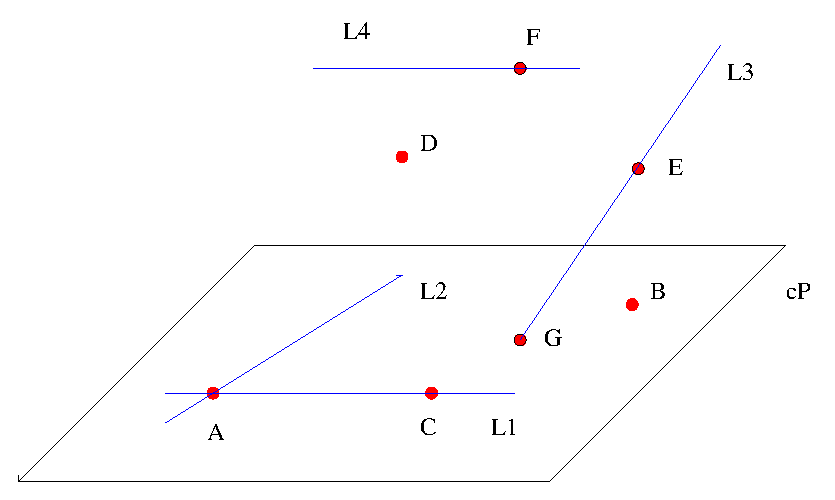
\includegraphics[height=2in]{../../modules/coordinate-systems/pictures/line_plane.eps}
  \caption{Points, lines, and planes}
  \label{fig:points_lines_planes}
\end{figure}
%
\end{frame}
%\begin{frame}
 \frametitle{Cylindrical coordinates}
\begin{columns}
\column{0.4\textwidth}
%
  \psfrag{P}{$P$}
  \psfrag{O}{$O$}  
  \psfrag{xp}{$x_P$} 
  \psfrag{yp}{$y_P$} 
  \psfrag{zp}{$z_P$}     
  \psfrag{rp}{$r_P$}
  \psfrag{thp}{$\theta_P$}
  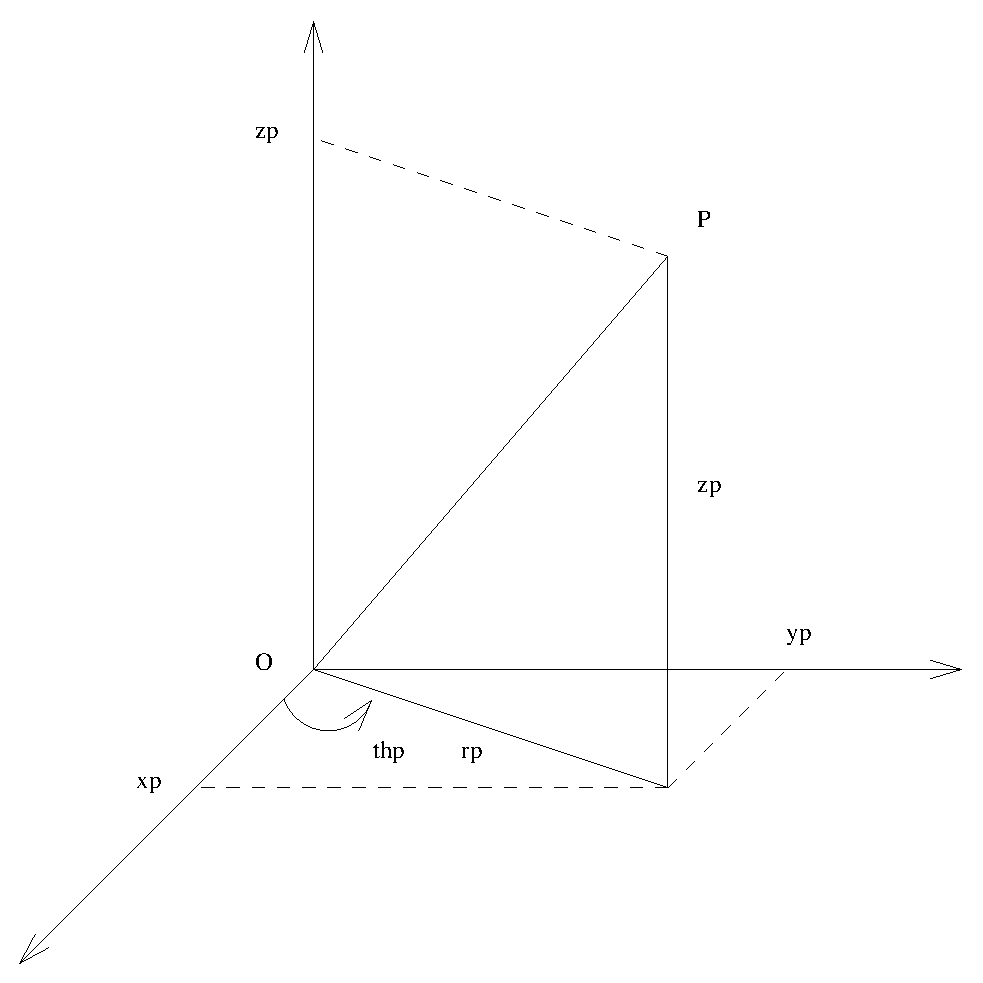
\includegraphics[height=2in]{../../modules/coordinate-systems/pictures/cylindrical_coordinates.eps}
  %\caption{Cylindrical coordinates}
  %\label{fig:cylindrical-coordinates}
%
\column{0.6\textwidth}
$$P(x,y,z) \Longleftrightarrow P(r, \theta, z)$$

\begin{itemize}
    \item Polar in $Oxy$ -- $(r, \theta)$;
    \item Rectangular in $Orz$ -- $(r, z)$.
\end{itemize}
\end{columns}

\end{frame}

\begin{frame}

\begin{columns}
\column{0.4\textwidth}
  \psfrag{P}{$P$}
  \psfrag{O}{$O$}  
  \psfrag{xp}{$x_P$} 
  \psfrag{yp}{$y_P$} 
  \psfrag{zp}{$z_P$}     
  \psfrag{rp}{$r_P$}
  \psfrag{thp}{$\theta_P$}
  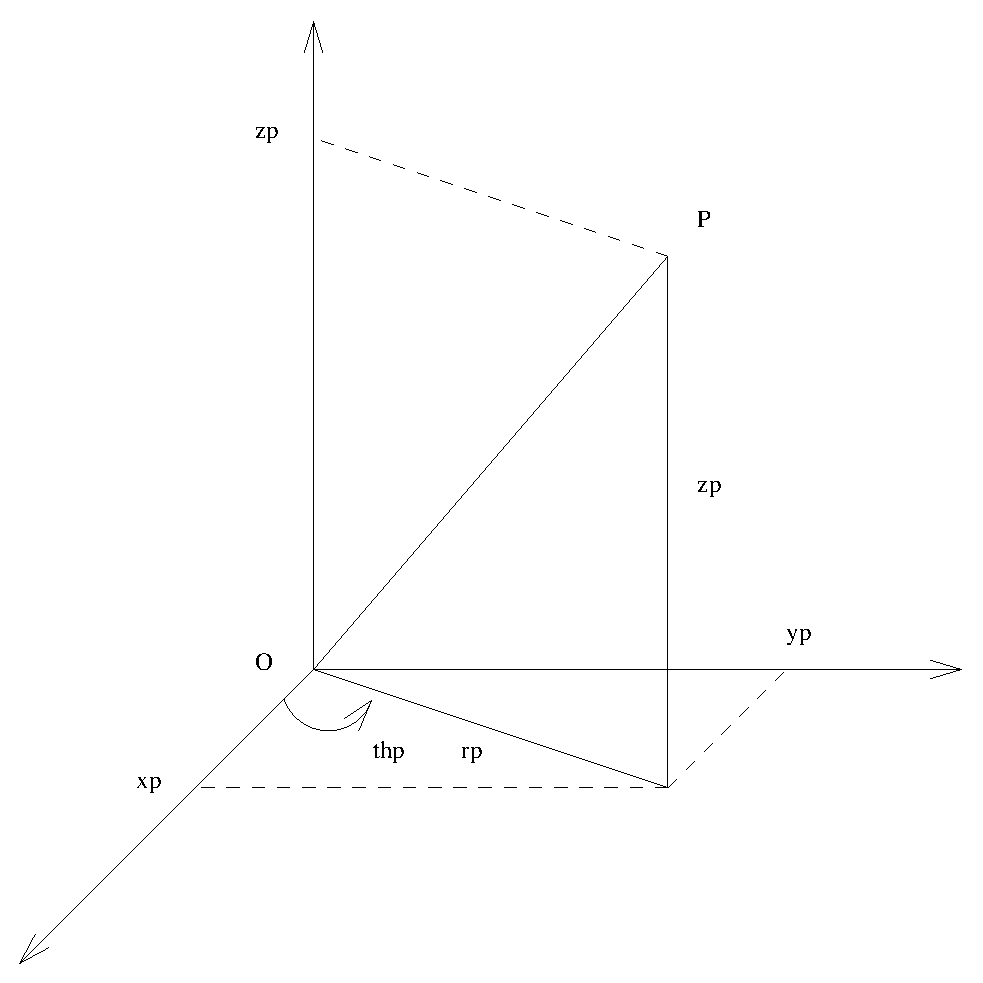
\includegraphics[height=2in]{../../modules/coordinate-systems/pictures/cylindrical_coordinates.eps}
  %\caption{Cylindrical coordinates}
  %\label{fig:cylindrical-coordinates}
%
\column{0.6\textwidth}
To transform cylindrical to rectangular coordinates:\pause
$$x=r\cos\theta \quad , \quad y = r\sin\theta \quad , \quad z_{r} = z_{c}$$

Rectangular to cylindrical:\pause
$$r= \sqrt{x^2+y^2} \quad , \quad z_{c}=z_{r}$$
$$\cos\theta = \frac{x}{r} \quad , \quad \sin\theta = \frac{y}{r}\; .$$
\end{columns}
\end{frame}

\begin{frame}
\frametitle{Constant Coordinate Sets}
\begin{columns}
\column{0.4\textwidth}
  \psfrag{P}{$P$}
  \psfrag{O}{$O$}  
  \psfrag{xp}{$x_P$} 
  \psfrag{yp}{$y_P$} 
  \psfrag{zp}{$z_P$}     
  \psfrag{rp}{$r_P$}
  \psfrag{thp}{$\theta_P$}
  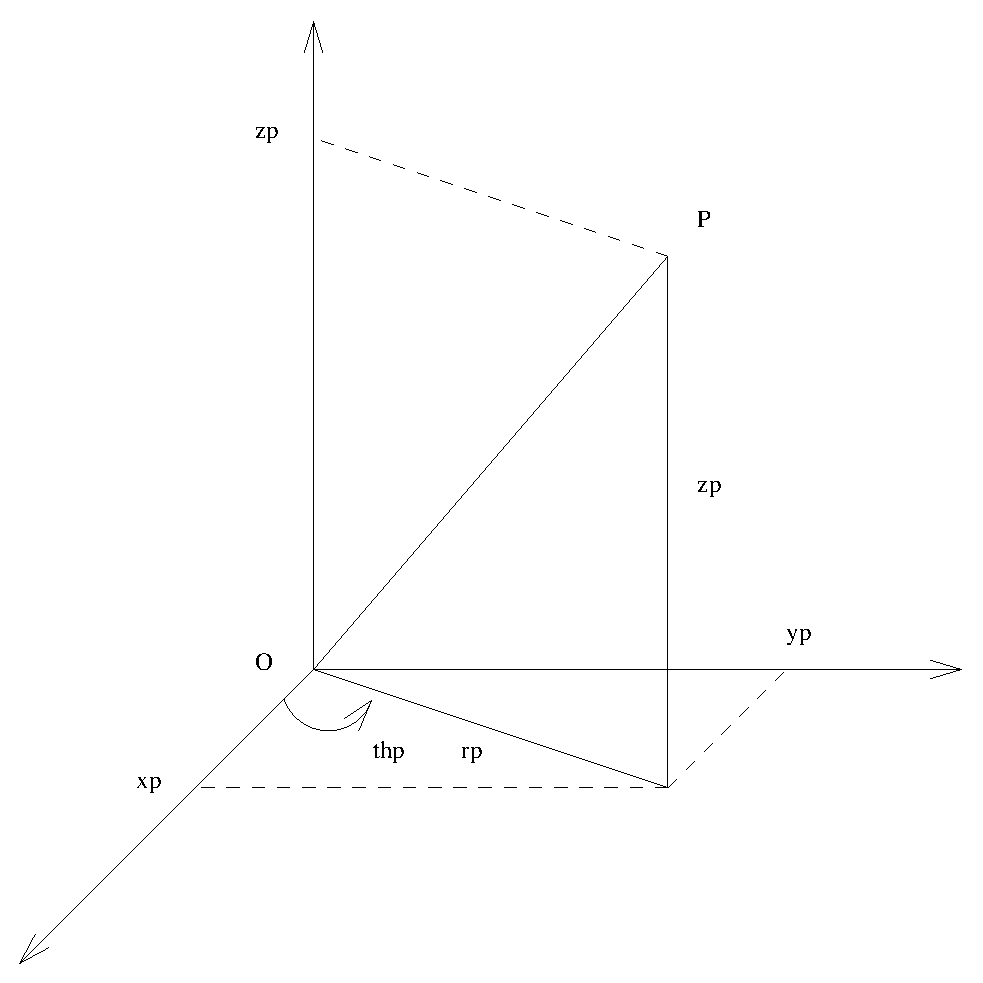
\includegraphics[height=2in]{../../modules/coordinate-systems/pictures/cylindrical_coordinates.eps}
\column{0.6\textwidth}

Surfaces:
\begin{itemize}
  \item $r$ constant \pause$\to$ vertical cylinder;
  \item $\theta$ constant \pause$\to$ vertical half plane;
  \item $z$ constant \pause$\to$ horizontal plane.\pause
\end{itemize}
%
Curves:
\begin{itemize}
 \item $\theta, z$ constant \pause$\to$ horizontal ray;
\item $r, z$ constant \pause$\to$ horizontal circle;
\item $r, \theta$ constant \pause$\to$ vertical line.
\end{itemize}
\end{columns}
\end{frame}
%\begin{frame}
 \frametitle{Spherical Coordinates}
\begin{columns}
\column{0.55\textwidth}
%  \psfrag{P}{$P$}
%  \psfrag{O}{$O$}
%  \psfrag{xp}{$x_P$}
%  \psfrag{yp}{$y_P$}
%  \psfrag{zp}{$z_P$}
%  \psfrag{rho}{$\rho_P$}
%  \psfrag{thp}{$\theta_P$}
%  \psfrag{phi}{$\phi_P$}
\psset{xunit=1cm, yunit=1cm}
\begin{pspicture}(-2.1,-2.5)(5,5.2)
\tiny
\renewcommand{\fcScreen}{[-1 -0.4 -0.25] -1}
\fcBoundingBox{-2.1}{-2.5}{2}{2}
\fcAxesIIId{5}{5}{5}
\fcPutIIId[r]{[0 -0.15 0.15]}{$O$}
\fcLineIIId[linestyle=dotted]{[3 0 0]}{[3 3 0]}
\fcLineIIId[linestyle=dotted]{[3 3 0]}{[0 3 0]}
\fcLineIIId[linestyle=dotted]{[0 0 0]}{[0 3 0]}
\fcLineIIId{[0 0 0]}{[3 3 0]}
\fcLineIIId{[3 3 0]}{[3 3 3]}
\fcLineIIId{[0 0 3]}{[3 3 3]}
\fcPutIIId[l]{[3.1 3.1 3.1]}{$P$}
\fcPutIIId[r]{[1.5 -0.1 0]}{$x_P$}
\fcPutIIId[t]{[3 3 0]}{$Q$}
\fcPutIIId[b]{[0 1.5 0]}{$y_P$}
\fcPutIIId[l]{[3 3 1.5]}{$~~z_P$}
\fcPutIIId[r]{[0 0 1.5]}{$z_P~~$}
\uncover<2->{%
\fcLineIIId{[0 0 0]}{[3 3 3]}
\uncover<3>{\fcLineIIId[linecolor=red, linewidth=2pt]{[0 0 0]}{[3 3 3]}}%
\fcPutIIId[r]{[2.1 2.1 2.1]}{$\rho_P$}
\fcPutIIId[rt]{[1 1 1.5]}{$\phi_P~~$}
\fcPutIIId[tr]{[1.8 0.9 0]}{$\theta_P$}%
\fcAngleIIId[linecolor=red, arrows=->]{[0 0 1]}{[3 3 3]}{1.7}%
\uncover<4>{\fcAngleIIId[linecolor=red, linewidth=2pt, arrows=->]{[0 0 1]}{[3 3 3]}{1.7}}%
\fcAngleIIId[linecolor=red, arrows=->]{[1 0 0]}{[3 3 0]}{1.7}%
\uncover<5>{\fcAngleIIId[linecolor=red, arrows=->, linewidth=2pt]{[1 0 0]}{[3 3 0]}{1.7}}%
}%
\uncover<8>{\fcLineIIId[arrows=->, linecolor=red, linewidth=2pt]{[0 0 0]}{[5 5 5]}}%
\uncover<10>{%
\fcAngleIIId[linecolor=red, linewidth=2pt]{[0 0 1]}{[1 1 0]}{2}%
\fcAngleIIId[linecolor=red, linewidth=2pt, arrows=->]{[1 1 0]}{[0 0 -1]}{2}%
}%
\uncover<12>{%
\fcAngleIIId[linecolor=red, linewidth=2pt]{[1 0 0]}{[0 1 0]}{2}%
\fcAngleIIId[linecolor=red, linewidth=2pt]{[0 1 0]}{[-1 0 0]}{2}%
\fcAngleIIId[linecolor=red, linewidth=2pt]{[-1 0 0]}{[0 -1 0]}{2}%
\fcAngleIIId[linecolor=red, linewidth=2pt, arrows=->]{[0 -1 0]}{[1 0 0]}{2}%
}%
\end{pspicture}
%  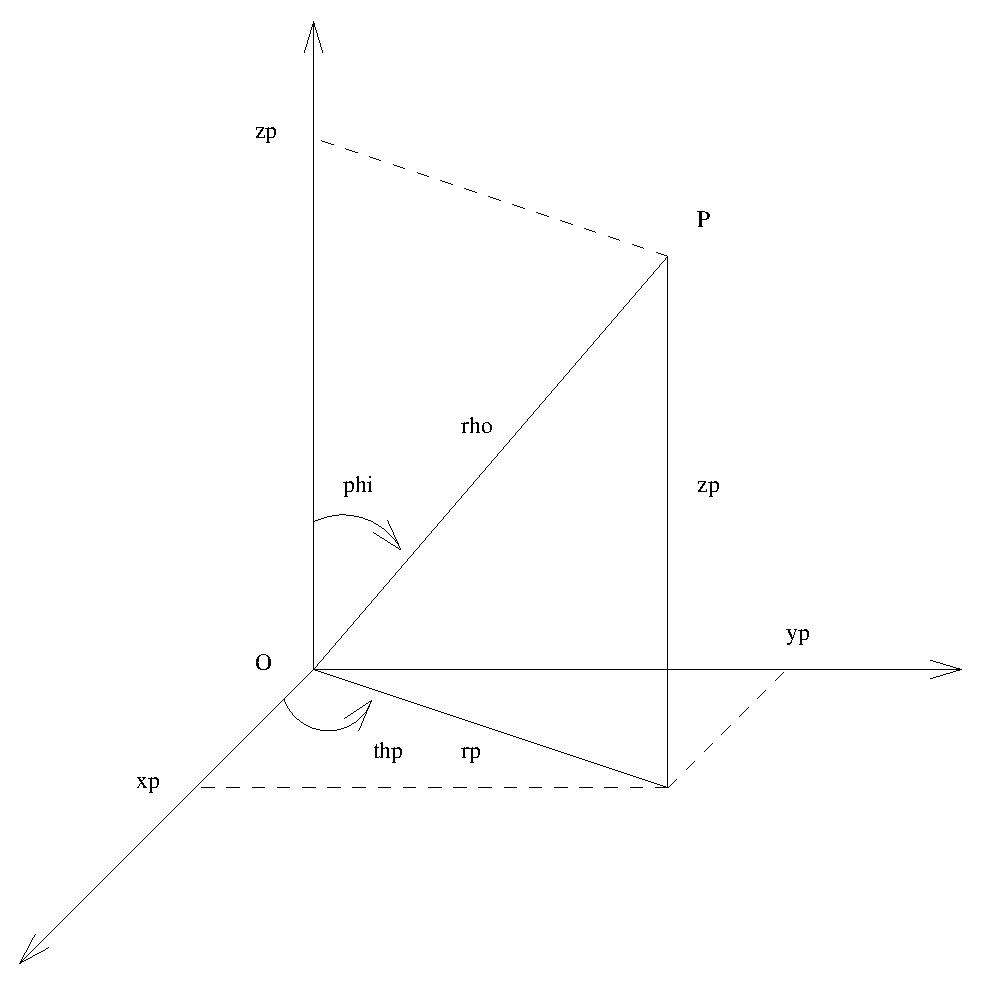
\includegraphics[height=2in]{../../modules/coordinate-systems/pictures/ok-cylindrical-spherical.eps}
\column{0.45\textwidth}
\begin{itemize}
\item In Cartesian coordinates, a point $P$ is given by triple $(x_P, y_P, z_P)$.
\item<2-> We introduce alternative spherical coordinates $(\rho_P, \phi_P,\theta_P)$.
\begin{itemize}
\item \alertNoH{3}{$\rho_P$: distance $|OP|$;}
\item \alertNoH{4}{$\phi_P$: angle $Oz$ to $OP$;}
\item \alertNoH{5}{$\theta_P$: angle $Ox$ to $OP_{xy}$.}
\end{itemize}
\item<6-> Coordinates range:
\begin{itemize}
\item \alertNoH{7,8}{$\rho$:} \uncover<8->{\alertNoH{8}{ $[0,\infty)$;}}
\item \alertNoH{9,10}{$\phi$:}  \uncover<10->{\alertNoH{10}{$[0, \pi]$;}}
\item \alertNoH{11,12}{$\theta$:}  \uncover<12->{ \alertNoH{12}{$[0,2\pi)$.}}
\end{itemize}
\end{itemize}
\end{columns}
\end{frame}

%\begin{frame}
\frametitle{Transition Spherical - Rectangular coordinates}
\begin{columns}
\column{0.4\textwidth}
\psset{xunit=1cm, yunit=1cm}
\begin{pspicture}(-3,-2)(2,2)
\tiny
\renewcommand{\fcScreen}{[-1 -0.4 -0.25] -1}
\fcLineIIId[arrows=->]{[0 0 0]}{[5 0 0 ]}
\fcLineIIId[arrows=->]{[0 0 0]}{[0 5 0 ]}
\fcLineIIId[arrows=->]{[0 0 0]}{[0 0 5 ]}
\fcPutIIId[r]{[0 -0.15 0.15]}{\alert<2,3,4>{$O$}}
\fcLineIIId[linecolor=gray]{[3 0 0]}{[3 3 0]}
\fcLineIIId[linecolor=gray]{[3 3 0]}{[0 3 0]}
\fcLineIIId{[0 0 0]}{[3 3 0]}
\fcLineIIId{[3 3 0]}{[3 3 3]}
\fcLineIIId{[0 0 0]}{[3 3 3]}
\fcLineIIId{[0 0 3]}{[3 3 3]}
\fcPutIIId[l]{[3.1 3.1 3.1]}{\alert<4>{$P$}}
\fcPutIIId[r]{[1.5 -0.1 0]}{$\alert<1>{x}$}
\fcPutIIId[t]{[3.1 3.1 0]}{\alert<2,3>{$Q$}}
\uncover<2->{\fcPutIIId[l]{[1.4 1.5 0]}{\alert<4,5,6>{$~~r$}}}
\uncover<2->{
\fcPutIIId[r]{[3 -0.1 0]}{\alert<2,3>{$S$}}
\fcPolyLineIIId[linecolor=red]{[2.6 0 0 ] [2.6 0.4 0] [3 0.4 0]}
}
\uncover<2->{
\fcPutIIId[b]{[-0.1 1.5 0]}{$y$}
\fcPutIIId[t]{[3.1 1.5 0]}{\alert<5>{$y$}}
}
\uncover<7->{\fcPutIIId[r]{[0 0 1.5]}{\alert<7>{$z~~$}}}
\uncover<4->{
\fcPutIIId[r]{[0 -0.1 3]}{\alert<4>{$T~$}}
\fcPutIIId[b]{[1.4 1.5 3]}{\alert<4,6>{$~~r$}}
\fcPolyLineIIId[linecolor=red]{[2.6 2.6 0] [2.6 2.6 0.56569] [3 3 0.56569]}
\fcPolyLineIIId[linecolor=red]{[0.4 0.4 3] [0.4 0.4 3 0.56569 sub] [0 0 3 0.56569 sub]}
}
\fcPutIIId[r]{[1.7 1.7 1.7]}{\alert<4,6,7>{$\rho~~$}}
\fcPutIIId[rt]{[0.8 0.8 1.3]}{\alert<4,6,7>{$\phi~~$}}
\fcPutIIId[br]{[1.2 0.5 0]}{\alert<3,5>{$\theta$}}
\fcCurveIIId[linecolor=red, arrows=->]{0}{54.74}{ %
t sin 45 cos mul 1.5 mul % 
t sin 45 sin mul 1.5 mul %
t cos 1.5 mul %
} %
\fcCurveIIId[linecolor=red, arrows=->]{0}{45}{ %
t cos 1.5 mul % 
t sin 1.5 mul %
0 %
} %
\end{pspicture} 
\column{0.6\textwidth}

From spherical to rectangular coords:
\[
\begin{array}{rcll|l}
\alert<1->{x}&\alert<1>{=}& \uncover<3->{\alert<3>{ \alert<4>{r}\cos\theta}} &&\uncover<2->{\alert<2,5>{ \text{use }\triangle SQO}} \\ 
\uncover<4->{&\alert<0>{=} & \alert<4>{\rho\sin\phi }\cos\theta &&\alert<4,6,7>{ \text{use }\triangle OPT} }\\
\uncover<5->{\alert<5>{y}&\alert<0>{=}& \alert<5>{\alert<6>{r} \sin\theta } }\\
\uncover<6->{&\alert<0>{=}& \alert<6>{\rho\sin\phi }\sin\theta} \\
\uncover<7->{\alert<7>{z}&\alert<7>{=}& \alert<7>{\rho\cos\phi }}
\end{array}
\]
\uncover<8->{
From rectangular to spherical coords:
$$\rho = \sqrt{x^2+y^2+z^2} \quad , \quad r = \sqrt{x^2+y^2}$$
$$\cos\phi = \frac{z}{\rho} \quad , \quad \sin\phi = \frac{r}{\rho}$$
$$\cos\theta = \frac{x}{r} \quad , \quad \sin\theta = \frac{y}{r}$$
}
\end{columns}
\end{frame}

\begin{frame}
 \frametitle{Curvilinear boxes}
 
 Polar ``wedge'':
 %
$$C  = \{ P(r,\theta) \; | \;r_0 \leqslant
r \leqslant r_0+\Delta r,  \theta_0 \leqslant \theta
\leqslant \theta_0+\Delta \theta\} \; .$$
%
Shape? \pause Area = ...?
\pause

\bigskip

Cylindrical ``box'':
%
$$X = \{ P(r,\theta, z) \; | \; 0 \leqslant r \leqslant r_0\, ,
0 \leqslant \theta \leqslant \theta_0\, ,
0 \leqslant z \leqslant z_0\}$$

\pause
Shape ? \pause Volume = ...?

\bigskip

\pause
Spherical ``box'':
%
$$Y = \{ P(\rho, \phi, \theta) \; | \; 0 \leqslant \rho \leqslant \rho_0\, ,
0 \leqslant \phi \leqslant \phi_0\, ,
0 \leqslant \theta \leqslant \theta_0\}$$

\pause
Shape? \pause Volume = ...?

\end{frame}
%\begin{frame}
\begin{pspicture}(-2,-2)(2,2)
%\pstVerb{[1 5 6]  \fcArrayToStack stack}
\pstVerb{[1 2 3] \fcProjectOntoScreen ==}
\pstVerb{[1 2 3] [4 5 6] \fcVectorMinusVector ==}
%\fcFullDot{1}{1}
%\pstVerb{[1 2 3] 5 \fcVectorTimesScalar \fcArrayToStack stack}
%\pscircle*[fillcolor=white, linecolor=red](! \fcProjectOriginOnPlane{1}{1}{1}{1}){0.07}
\end{pspicture}
\end{frame}
%\begin{frame}
Looking for $t $ such that 
\[
\begin{array}{rcl}
\displaystyle\langle \mathbf{v}+t \mathbf{n}, \mathbf{n}\rangle  &=&\displaystyle d\\
\displaystyle t&=&\displaystyle \frac{d-\langle\mathbf{v},\mathbf{n} \rangle}{\langle\mathbf{n}, \mathbf{n} \rangle}
\end{array}
\]
\begin{pspicture}(-2,-2)(2,2)
%\pstVerb{[1 5 6]  \fcArrayToStack stack}

\pstVerb{[1 2 3] [4 5 6] 7 \fcProjectOntoPlane \fcArrayToStack stack}

%\pstVerb{[1 2 3] 5 \fcVectorTimesScalar \fcArrayToStack stack}
%\pscircle*[fillcolor=white, linecolor=red](! \fcProjectOriginOnPlane{1}{1}{1}{1}){0.07}


\end{pspicture}
\end{frame}
%\begin{frame}
\begin{pspicture}(-2,-2)(2,2)
\fcAxesIIId{2}{2}{2}
\end{pspicture}
\end{frame}
%

\begin{frame}


\psset{xunit=1cm, yunit=1cm}
\stripPoints{\psxunit}
\stripPoints{\psyunit}

\begin{pspicture}(0,0)(1,1)
\psline(0,1)(7,1)
\fcLine{[0 0]}{[7 0]}
\pstVerb{
\fcCurve{0}{3600}{[t cos t sin]}
}
%\fcLine{[0 0]}{[100 -200]}
%\fcLine{[0 0]}{[100 90]}
%\fcLine{[0 0]}{[100 -90]}
\end{pspicture}
%\begin{pspicture}(-1,-1)(1,1)
%\end{pspicture}

\end{frame}
%\begin{frame}

\psset{xunit=0.4cm, yunit=0.4cm}
\begin{pspicture}(-5,-5)(5,5)
\fcAxesStandard{-5}{-5}{5}{5}
\fcVectorField[linecolor=blue, arrows=->]{-5}{-5}{11}{11}{1}{1 dict begin /r x x mul y y mul add sqrt def  r 0 eq {0 0} {-1 y mul r div  x r div} ifelse end}
\end{pspicture}

\end{frame}

%%\begin{comment}
\begin{frame}
\frametitle{A motivating example}
$
\displaystyle g(x,y) =x^2+2y^2
$

\begin{itemize}
\item What does the graph $\Gamma$ of $g$ look like?
\item<2-> $\Gamma$ = points in $\RR^3$ such that $z=x^2+2y^2$. The set is not a plane: what does it look like?
\item<3-> To answer look at sections. Use imaginary CT scan to cut the graph; assemble resulting sections into a graph.
\end{itemize}

\vskip 10cm
\end{frame}

\begin{frame}
\frametitle{A motivating example}
$
g(x,y) =x^2+2y^2
$

\begin{columns}
\column{0.4\textwidth}
\centering

\psset{xunit=0.75cm, yunit=0.75cm}
\begin{pspicture}(-3.4,-2)(3,4.3)
\tiny
\fcBoundingBox{-3.4}{-1.3}{3}{4.35}
\renewcommand{\fcScreen}{[-1 1 -0.5] -1}
\psline[linecolor=red!1](3, 4.3)(3.01,4.31)%
\psline[linecolor=red!1](-3.4, -1)(-3.41,-1.01)%
\uncover<2-5,9>{\fcParallelogramIIId{[1 -1.2 -0.5]}{[1 1.2 -0.5]}{[1 -1.2 4]}}%
\uncover<6>{\fcParallelogramIIId{[0 -1.2 -0.5]}{[0 1.2 -0.5]}{[0 -1.2 4]}} %
\uncover<7>{\fcParallelogramIIId{[0.333333 -1.2 -0.5]}{[0.333333 1.2 -0.5]}{[0.333333 -1.2 4]}} %
\uncover<8>{\fcParallelogramIIId{[0.666666 -1.2 -0.5]}{[0.666666 1.2 -0.5]}{[0.666666 -1.2 4]}} %
\fcAxesIIId{3}{3}{3}
\uncover<11->{\fcLineIIId[arrows=->, linecolor=black]{[0 0 0]}{[-3 0 0]}}
%parabola at x=1
\uncover<4-5,9->{\fcCurveIIId{-1.2}{1.2}{[1 t 2 t t mul mul 1 add]}} %
\uncover<5,9,10,12>{\fcDotIIId{[1 0 1]}} %
\uncover<2-5,9>{%
\fcDotIIId[linecolor=black]{[1 0 0]} %
\fcPutIIId[t]{[1 0 -0.3]}{$~~a$}%
} %
\uncover<5>{\fcPutIIId[bl]{[1 0 1.3]}{$~~~~\left(a,0,a^2\right)$}}%
%parabola at x=0
\uncover<6,10->{\fcCurveIIId{-1.2}{1.2}{[0 t 2 t t mul mul 0 add]}}
\uncover<6,10,12>{\fcDotIIId{[0 0 0]}}
\uncover<6>{ %
\fcDotIIId[linecolor=black]{[0 \space 0 0]}%
\fcPutIIId[t]{[0 0 -0.3]}{$~~a=0$}%
} %
%parabola at x=1/3
\uncover<7>{\fcCurveIIId{-1.2}{1.2}{[0.333333 t 2 t t mul mul 0.333333 dup mul add]}}
\uncover<7>{\fcDotIIId{[0.333333 0 0.333333 0.333333 mul]}}
\uncover<7>{ %
\fcDotIIId[linecolor=black]{[0.333333 0 0]}%
\fcPutIIId[t]{[0.333333 0 -0.3]}{$~~a$}%
}
%parabola at x=1/2
\uncover<10->{\fcCurveIIId{-1.2}{1.2}{[0.5 t 2 t t mul mul 0.5 dup mul add]}}
\uncover<10>{\fcDotIIId{[0.5 0 0.5 dup mul]}}
%parabola at x=2/3
\uncover<8>{\fcCurveIIId{-1.2}{1.2}{[0.666666 t 2 t t mul mul 0.666666 dup mul add]}}%
\uncover<8>{\fcDotIIId{[0.666666 0 0.666666 0.666666 mul]}}
\uncover<8>{ %
\fcDotIIId[linecolor=black]{[0.666666 0 0]}%
\fcPutIIId[t]{[0.666666  0 -0.3]}{$~~a$}%
} %
\uncover<11->{
%\fcCurveIIId{-1.2}{1.2}{[-0.333333 t 2 t t mul mul 0.333333 dup mul add]}
\fcCurveIIId{-1.2}{1.2}{[-0.5 t 2 t t mul mul 0.5 dup mul add]}
\fcCurveIIId{-1.2}{1.2}{[-1.0 t 2 t t mul mul 1.000000 dup mul add]}
}
\uncover<12>{
\fcCurveIIId[linecolor=blue]{-1.5}{1.5}{[t 0 t t mul]}
\fcDotIIId{[-0.5 0  -0.5 dup mul]}
\fcDotIIId{[0.5 0  0.5 dup mul]}
\fcDotIIId{[-1.000000 0  -1.000000 dup mul]}
}
\end{pspicture}

\uncover<2->{
\psset{xunit=0.4cm, yunit=0.4cm}
\begin{pspicture}(-1.6, -0.9)(1.6,4.38)
\tiny
\psframe*[linecolor=cyan!30](! -1.45 -0.75)(! 1.45 4.13)%
\psaxes[ticks=none, labels=none]{<->}(0,0)(-1.35,-0.65)(1.35,4.03)
\fcLabels[$y$][$z$]{1.35}{4.03}

\uncover<6>{
%Function formula: 2 x^{2}
\psplot[linecolor=\fcColorGraph, plotpoints=1000]{-1.2}{1.2}{x 2 exp 2 mul }
\fcFullDot{0}{0}
}

\uncover<7>{
%Function formula: 2 x^{2}+\frac{1}{9}
\psplot[linecolor=\fcColorGraph, plotpoints=1000]{-1.2}{1.2}{ 0.111111 x 2 exp 2 mul add }
\fcFullDot{0}{0.111111}
}
\uncover<8>{
%Function formula: 2 x^{2}+\frac{4}{9}
\psplot[linecolor=\fcColorGraph, plotpoints=1000]{-1.2}{1.2}{ 0.444444 x 2 exp 2 mul add }
\fcFullDot{0}{0.444444}
}
\uncover<3-5, 9->{ %
%Function formula: 2 x^{2}+1
\psplot[linecolor=\fcColorGraph, plotpoints=1000]{-1.2}{1.2}{ 1 x 2 exp 2 mul add } %
} %
\uncover<5, 9->{\fcFullDot{0}{1}} %
\end{pspicture}

The plane $x=a$.

\vskip 3cm %for alignment
} % uncover end

\column{0.6\textwidth}
\begin{itemize}
\item<2-> Cut by vertical planes $x=a$, $a$-constant, parallel to the $Oyz-$plane.
\item<3-> In other words, treat $x$ as constant and study the f-n $y\to z= a^2+2y^2=g(a,y) $.

\item<4-> The cross-sections are the curves:
$
\displaystyle \{(a, y, z)\quad \text{where } z=a^2+2y^2\}
$
\item<5-> These are parabolas lying inside the plane $x=a$ with vertices at $\left(a,0,a^2\right)$.

\item<6-> As $a$ moves away from $0$, the parabola vertex rises.
\item<12-> The vertices traverse the curve given by $\{ (a, 0, a^2) \}$.
\end{itemize}
\end{columns}

\vskip 10 cm
\end{frame}
%\end{comment}

%\begin{comment}
\begin{frame}
\frametitle{A motivating example}
$
g(x,y) =x^2+2y^2
$

\begin{columns}
\column{0.4\textwidth}
\centering
\psset{xunit=0.75cm, yunit=0.75cm}
\begin{pspicture}(-3.4,-2)(3,4.3)
\tiny
\fcBoundingBox{-3.4}{-1.3}{3}{4.35}
\renewcommand{\fcScreen}{[-1 1 -0.5] -1}
\psline[linecolor=red!1](3, 4.3)(3.01,4.31)%
\psline[linecolor=red!1](-3.4, -1)(-3.41,-1.01)%
%parabola at y=1
\uncover<1-3,7>{\fcParallelogramIIId{[-1  1 -0.5]}{[1 1 -0.5]}{[-1 1 4]}}%
\uncover<1-3,7>{ %
\fcDotIIId[linecolor=black]{[0 1 0]}%
\fcPutIIId[t]{[0 1 -0.3]}{$~~a$}%
} %
\uncover<3,7->{\fcCurveIIId{-1}{1}{[t 1 2 t t mul mul 1 dup mul 2 mul add]}} %

%parabola at y=0
\uncover<4>{\fcParallelogramIIId{[-1  0 -0.5]}{[1 0 -0.5]}{[-1 0 4]}}%
\uncover<4>{ %
\fcDotIIId[linecolor=black]{[0 0 0]}%
\fcPutIIId[t]{[0 0 -0.3]}{$~~a$}%
} %
\uncover<4,8->{\fcCurveIIId{-1}{1}{[t 0 2 t t mul mul 0 dup mul 2 mul add]}} %

%parabola at y=1/3
\uncover<5>{\fcParallelogramIIId{[-1  0.333333 -0.5]}{[1 0.333333 -0.5]}{[-1 0.333333 4]}}%
\uncover<5>{%
\fcDotIIId[linecolor=black]{[0 0.333333 0]}%
\fcPutIIId[t]{[0 0.333333 -0.3]}{$~~a$}%
} %
\uncover<5>{\fcCurveIIId{-1}{1}{[t 0.333333 2 t t mul mul 0.333333 dup mul 2 mul add]}} %

%parabola at y=2/3
\uncover<6>{\fcParallelogramIIId{[-1  0.666666 -0.5]}{[1 0.666666 -0.5]}{[-1 0.666666 4]}}%
\uncover<6>{ %
\fcDotIIId[linecolor=black]{[0 0.666666 0]}%
\fcPutIIId[t]{[0 0.666666 -0.3]}{$~~a$}%
} %
\uncover<6,8->{\fcCurveIIId{-1}{1}{[t 0.666666 2 t t mul mul 0.666666 dup mul 2 mul add]}} %

\fcAxesIIId{3}{3}{3}%
\uncover<9->{%
\fcLineIIId[arrows=->]{[0 0 0]}{[0 -3 0]} %
\fcCurveIIId{-1}{1}{[t -0.666666 2 t t mul mul 0.666666 dup mul 2 mul add]} %
\fcCurveIIId{-1}{1}{[t -1 2 t t mul mul 1 dup mul 2 mul add]}%
}%
\uncover<10->{%
\fcCurveIIId[linecolor=blue]{-1.2}{1.2}{[0 t 2 t t mul mul]}%
\fcDotIIId{[0 0 0]}%
\fcDotIIId{[0 -0.5 0.5]}%
\fcDotIIId{[0 0.5 0.5]}%
\fcDotIIId{[0 1 2]}%
\fcDotIIId{[0 -1 2]}%
}
\end{pspicture}

\uncover<1->{
\psset{xunit=0.4cm, yunit=0.4cm}
\begin{pspicture}(-1.6, -0.9)(1.6,4.38)
\tiny
\psframe*[linecolor=cyan!30](! -1.45 -0.75)(! 1.45 4.13)%
\psaxes[ticks=none, labels=none]{<->}(0,0)(-1.35,-0.65)(1.35,4.03)
\fcLabels[$x$][$z$]{1.35}{4.03}
\uncover<4>{
%Function formula: 2 x^{2}
\psplot[linecolor=\fcColorGraph, plotpoints=1000]{-1}{1}{x 2 exp 2 mul }
}%
\uncover<5>{%
%Function formula: 2 x^{2}+\frac{2}{9}
\psplot[linecolor=\fcColorGraph, plotpoints=1000]{-1}{1}{ 2 9 div x 2 exp 2 mul add }%
}%
\uncover<6>{%
%Function formula: 2 x^{2}+2*\frac{4}{9}
\psplot[linecolor=\fcColorGraph, plotpoints=1000]{-1}{1}{ 8 9 div x 2 exp 2 mul add }%
}%
\uncover<3, 7->{%
%Function formula: 2 x^{2}+1
\psplot[linecolor=\fcColorGraph, plotpoints=1000]{-1}{1}{ 2 x 2 exp 2 mul add }%
}%
\end{pspicture}

The plane $x=a$.
%\vskip 3cm %for alignment
} % uncover end

\column{0.6\textwidth}
\begin{itemize}
\item<1-> Similarly, cut by vertical planes $y=a$, i.e., planes parallel to the $Oxz$ plane.

\item<2-> In other words, treat $y$ as constant and study the f-n $z=g(x,a) = x^2+2a^2$.

\item<3-> The cross-sections are the curves  $\{ (x,a,z) \text{  where  } z= x^2+2a^2\}$. These are parabolas lying inside the plane $y=a$.
\item<8-> $\Rightarrow$ the vertical sections along both the $x$ and $y$ axes are parabolas.
\item<10-> The vertices are rising as we move away from the origin.
\end{itemize}
\vskip 2.4cm
\end{columns}

\vskip 10 cm
\end{frame}
%\end{comment}


%\begin{comment}
\begin{frame}

\frametitle{A motivating example}
$
g(x,y) =x^2+2y^2
$

\begin{columns}
\column{0.4\textwidth}
\centering
\psset{xunit=0.65cm, yunit=0.65cm}
\begin{pspicture}(-4,-2.2)(3,4)
\tiny
\fcBoundingBox{-3.5}{-1.3}{3.5}{4.3}
\renewcommand{\fcScreen}{[-1 1 -0.5] -1}
\psline[linecolor=red!1](3, 4)(3.01,4.01)%
\psline[linecolor=red!1](-3, -2.2)(-3.01,-2.21)%
\uncover<1-2>{ %
\fcParallelogramIIId{[-2.5  -2.5 1]}{[2.5 -2.5 1]}{[-2.5 2.5 1]}
\fcDotIIId[linecolor=black]{[0 0 1]}%
\fcPutIIId[tl]{[0 0 1]}{$~~a$}%
} %
\uncover<3>{ %
\fcParallelogramIIId{[-2.5  -2.5 -1]}{[2.5 -2.5 -1]}{[-2.5 2.5 -1]}
\fcDotIIId[linecolor=black]{[0 0 -1]}%
\fcPutIIId[tl]{[0 0 -1]}{$~~a$}%
} %
\uncover<4>{ %
\fcParallelogramIIId{[-2.5  -2.5 0]}{[2.5 -2.5 0]}{[-2.5 2.5 0]}
} %
\uncover<5>{ %
\fcParallelogramIIId{[-2.5  -2.5 0.5]}{[2.5 -2.5 0.5]}{[-2.5 2.5 0.5]}
} %
\uncover<6>{ %
\fcParallelogramIIId{[-2.5  -2.5 1]}{[2.5 -2.5 1]}{[-2.5 2.5 1]}
} %
\uncover<7>{ %
\fcParallelogramIIId{[-2.5  -2.5 1.5]}{[2.5 -2.5 1.5]}{[-2.5 2.5 1.5]}
} %
\uncover<8>{ %
\fcParallelogramIIId{[-2.5  -2.5 2]}{[2.5 -2.5 2]}{[-2.5 2.5 2]}
} %

\fcAxesIIId{3}{3}{3}%
\fcLineIIId[arrows=->]{[0 0 0]}{[0 -3 0]} %
\fcLineIIId[arrows=->]{[0 0 0]}{[-3 0 0]} %
\fcLineIIId[arrows=->]{[0 0 0]}{[0 0 -1.5]} %

\uncover<4>{\fcDotIIId{[0 0 0]}}
\uncover<5,9->{ %
\fcCurveIIId{ 0}{6.2832}{[t 360 mul cos 0.500 sqrt mul t 360 mul sin 0.500 2 div sqrt mul 0.5]}
}
\uncover<5>{\fcDotIIId[linecolor=black]{[0 0 0.5]}}
\uncover<6,9->{ %
\fcCurveIIId{ 0}{6.2832}{[t 360 mul cos 1 sqrt mul t 360 mul sin 1 2 div sqrt mul 1]}
}
\uncover<6>{\fcDotIIId[linecolor=black]{[0 0 1]}}
\uncover<7,9->{ %
\fcCurveIIId{ 0}{6.2832}{[t 360 mul cos 1.5 sqrt mul t 360 mul sin 1.5 2 div sqrt mul 1.5]}
}
\uncover<7>{\fcDotIIId[linecolor=black]{[0 0 1.5]}}
\uncover<8,9->{ %
\fcCurveIIId{ 0}{6.2832}{[t 360 mul cos 2.0 sqrt mul t 360 mul sin 2.0 2 div sqrt mul 2.0]}
}
\uncover<8>{\fcDotIIId[linecolor=black]{[0 0 2.0]}}

\uncover<10->{
\fcCurveIIId[linewidth=1pt, linecolor=blue]{-1.414214 }{1.414214}{[t 0 t t mul]}
\fcCurveIIId[linewidth=1pt, linecolor=blue]{-1}{1}{[0 t t t 2 mul mul]}
}
\uncover<11->{
\fcCurveIIId[linewidth=2pt, linecolor=\fcColorGraph]{ 0}{6.2832}{[t 360 mul cos 0.500 sqrt mul t 360 mul sin 0.500 2 div sqrt mul 0.5]}
\fcCurveIIId[linewidth=2pt, linecolor=\fcColorGraph]{ 0}{6.2832}{[t 360 mul cos 1 sqrt mul t 360 mul sin 1 2 div sqrt mul 1]}
\fcCurveIIId[linewidth=2pt, linecolor=\fcColorGraph]{ 0}{6.2832}{[t 360 mul cos 1.5 sqrt mul t 360 mul sin 1.5 2 div sqrt mul 1.5]}
\fcCurveIIId[linewidth=2pt, linecolor=\fcColorGraph]{ 0}{6.2832}{[t 360 mul cos 2.0 sqrt mul t 360 mul sin 2.0 2 div sqrt mul 2.0]}
}
\end{pspicture}

\uncover<2->{
\psset{xunit=0.4cm, yunit=0.4cm}
\begin{pspicture}(-3.228413, -1.814212)(3.228427,1.914212)
\tiny
\psframe*[linecolor=cyan!30](! -3.078413 -1.664212)(! 3.078427 1.664212)%
\psaxes[ticks=none, labels=none]{<->}(0,0)(-2.978413,-1.564212) (2.978427,1.564212)
\fcLabels[$x$][$y$]{2.978427}{1.564212}
\uncover<4>{
\fcFullDot{0}{0}
}
\uncover<5>{
%Calculator input: plotCurve{}\left(\frac{\sqrt{2}}{2} \cos{}t, \frac{1}{2} \sin{}t, 0, 2 \pi\right)
\parametricplot[linecolor=\fcColorGraph, plotpoints=1000]{0}{6.28319}{t 57.29578 mul cos 0.707107 mul t 57.29578 mul sin 0.5 mul }
}
\uncover<6>{
%Calculator input: plotCurve{}\left(\cos{}t, \frac{\sqrt{2}}{2} \sin{}t, 0, 2 \pi\right)
\parametricplot[linecolor=\fcColorGraph, plotpoints=1000]{0}{6.28319}{t 57.29578 mul cos t 57.29578 mul sin 0.707107 mul }
}
\uncover<7>{
%Calculator input: plotCurve{}\left(\frac{\sqrt{2}\sqrt{3}}{2} \cos{}t, \frac{\sqrt{3}}{2} \sin{}t, 0, 2 \pi\right)
\parametricplot[linecolor=\fcColorGraph, plotpoints=1000]{0}{6.28319}{t 57.29578 mul cos 1.224745 mul t 57.29578 mul sin 0.866025 mul }
}
\uncover<8->{
%Calculator input: plotCurve{}\left(\sqrt{2} \cos{}t, \sin{}t, 0, 2 \pi\right)
\parametricplot[linecolor=\fcColorGraph, plotpoints=1000]{0}{6.28319}{t 57.29578 mul cos 1.414214 mul t 57.29578 mul sin }
}
\end{pspicture}

$x^2+2y^2= \only<1-3>{a} \only<4>{\alert<4>{0}}$, \only<1-3>{\alert<5>{$a<0$}}\only<5->{\alert<5>{$a>0$}}.
}

\column{0.6\textwidth}
\begin{itemize}
\item<1-> For horizontal sections keep constant the output variable, $z=a$.
\item<2-> When we intersect with $z=a$ we get the curve with equations $x^2+2y^2=a$, $z=a$.
\item<3-> For $a<0$ intersection is empty.
\item<4-> For $a=0$ intersection is $(0,0,0)$.
\item<5-> For $a>0$ intersection is an ellipse.
\item<10-> Figure is called ellipsoidal paraboloid.
\end{itemize}
\uncover<11->{
\begin{definition}
The sets $\{ (x,y,a)| g(x,y)=a\}$ are called \alert<11>{level curves} of the function $g$.
\end{definition}
}
\end{columns}

\vskip 10 cm
\end{frame}
\begin{frame}

\begin{itemize}
\item
You should be familiarized with level curves if you have ever seen a topographic map or from weather reports on the tv.
\item What are the functions in those cases?
\end{itemize}
\end{frame}
%\end{comment}

%\begin{frame}
\begin{itemize}
\item<1-> Previously we considered functions $\alertNoH{2,6}{z}= g(\alertNoH{3,5}{x,y})$  \alertNoH{2}{with scalar output} and \alertNoH{3}{two dimensional input}.
\item<4-> The graphs of such functions live in $\RR^3 = \RR^{\alertNoH{5}{2} +\alertNoH{6}{1}}$.
\item<5-> \alertNoH{5}{2 dimensions} were used to represent the input.
\item<6-> \alertNoH{6}{1 dimension} was used to represent the output.
\item<7-> To represent functions with 3 dimensional input (3 variables) and scalar output: need  $3+1=4$ dimensions.
\item<8-> That's difficult for eyes used to visualizing physical 3d- space.
\item<9-> Instead: label the level sets of the function with color or other means to indicate value.
\item<10-> In this way we represent the f-n graphically using dimension equal to the number of input variables.
\end{itemize}
\end{frame}
\begin{frame}
\frametitle{Example}
\begin{columns}
\column{0.4\textwidth}
\psset{xunit=0.4cm, yunit=0.4cm}
\begin{pspicture}(-4,-7)(6,10)
\renewcommand{\fcScreen}{[-1 1 -0.7] -1}
\fcBoundingBox{-4}{-8.5}{4}{10.5}
\tiny
\fcAxesIIIdFull{5}{5}{5}%
\uncover<5->{%
%d=4
\fcParallelogramIIId[linecolor=cyan!90]{[-2 -2 -8]}{[-2 3 -3]}{[5 -2 -1]}%
\fcPutIIId[l]{[2 2 0]}{$~~d=4$}%
\fcLineIIId{[0 0 0]}{[0 0 -4]}
\fcLineIIId{[0 0 0]}{[4 0 0]}
}%
\uncover<6->{%
%d=2
\fcParallelogramIIId[linecolor=cyan!70]{[-2 -2 -6]}{[-2 3 -1]}{[5 -2 1]}%
\fcPutIIId[l]{[2 2 2]}{$~~d=2$}%
\fcLineIIId{[0 0 0]}{[0 2 0]}
\fcLineIIId{[0 0 0]}{[2 0 0]}
\fcLineIIId{[0 0 0]}{[0 0 -2]}
}%
\uncover<7->{%
%d=0
\fcParallelogramIIId[linecolor=cyan!50]{[-2 -2 -4]}{[-2 3 1]}{[5 -2 3]}%
\fcPutIIId[l]{[2 2 4]}{$~~d=0$}%
\fcLineIIId{[0 0 0]}{[0 0 4]}
\fcLineIIId{[0 0 0]}{[-4 0 0]}
\fcLineIIId{[0 0 0]}{[0 -4 0]}
}%
\uncover<8->{%
%d=-2
\fcParallelogramIIId[linecolor=cyan!30]{[-2 -2 -2]}{[-2 3 3]}{[5 -2 5]}%
\fcPutIIId[l]{[2 2 6]}{$~~d=-2$}%
\fcLineIIId{[0 0 2]}{[0 0 4]}%
\fcLineIIId{[-2 0 0]}{[-4 0 0]}%
\fcLineIIId{[0 -2 0]}{[0 -5 0]}%
}%
\uncover<9->{%
%d=-4
\fcParallelogramIIId[linecolor=cyan!10]{[-2 -2 0]}{[-2 3 5]}{[5 -2 7]}%
\fcPutIIId[l]{[2 2 8]}{$~~d=-4$}
\fcPutIIId[l]{[2 2 6]}{$~~d=-2$}%
\fcLineIIId{[0 0 4]}{[0 0 5]}%
\fcLineIIId{[-4 0 0]}{[-5 0 0]}%
}%
\fcAxesIIIdFull[arrows=->, linestyle=dotted, dash=1pt]{5}{5}{5}
\end{pspicture}

\column{0.6\textwidth}
\begin{itemize}
\item<1-> Let $f(x,y,z) = x+y-z$.
\item<2-> The graph consists of the quadruples $(x,y,z,w)$ in $\RR^4$ such that $w = x+y-z$. Can't plot that graphically (yet).
\item<3-> However, can represent with labeled level sets.
\item<4-> The level set $f(x,y,z) = d$ is the surface $x+y-z = d$ in $\RR^3$, and that surface is a plane.
\item<5-> For varying values of $d$ we plot the level set.
$f(x,y,z) =d \onlyNoH{5}{=4}\onlyNoH{6}{=2} \onlyNoH{7}{=0}\onlyNoH{8}{=-2}
\onlyNoH{9}{=-4}$.

Darker color = larger $d$.
\end{itemize}
\end{columns}

\end{frame}

\begin{frame}
To understand surfaces in space we need the following.
\begin{remark} The level set $f(x,y,z)=0$ for the function
%
$$f(x,y,z) = ax+by-z+d$$
%
is the same as the graph of the function $g(x,y) = ax+by+c$.
\end{remark}
\begin{itemize}
\item<2-> Graph surfaces can always be represented as level surfaces
\item<3-> The converse is not true: level surfaces can't always be represented as graph surfaces.
\item<4-> Example: a sphere centered at the origin is the
level surface of $f(x,y,z) = x^2+y^2+z^2$ but it ``fails the vertical line test in all directions'', so it cannot be globally represented as a graph surface, no matter how we change the coordinate system.
\item<5-> We'll show that under reasonable assumptions, level surfaces can \emph{locally} be described as graph surfaces.
\end{itemize}
\end{frame}

%\begin{frame}
\frametitle{Vector fields}
\begin{itemize}
\item \emph{Vector fields} are functions with multidimensional input and output. 
\item Input is point in space; output is a vector, which we plot as a vector with a tail at the input point. 
\item Examples
\begin{itemize}
  \item Velocity of fluid/air at given point;
  \item Electric force per unit of charge;
  \item Gravitational field;
  %\item Fundamental directions $\textbf{e}_\rho$, $\textbf{e}_\phi$, $\textbf{e}_\theta$, $\textbf{e}_r$
\end{itemize}
\end{itemize}
\end{frame}

\begin{frame}
\frametitle{Coordinate representation of vector fields}

\begin{itemize}
\item<1-> In rectangular coordinates a vector field $\textbf{F}$ can
be decomposed along the fundamental directions:
$$
\textbf{F}(x,y,z) = F_1(x,y,z) \textbf{i} + F_2(x,y,z) \textbf{j} + F_3(x,y,z) \textbf{k} \; .
$$
\item<2-> For regions in the plane 2-dim vector fields are defined in a similar fashion: as function from subsets of $\mathbb R^2$ to $\RR$:
$$
\textbf{F}(x,y) = F_1(x,y) \textbf{i} + F_2(x,y) \textbf{j}
$$


\end{itemize}
\end{frame}
\begin{frame}
\begin{itemize}
\item<1-> Example: define the vector field $\textbf{e}_r$ on $\mathbb{R}^2 \setminus \{ (0,0)\}$ via
\[
\textbf{e}_r = \cos\theta\, \textbf{i} +
\sin\theta \,\textbf{j} = \frac{x}{r} \, \textbf{i} +
\frac{y}{r} \, \textbf{j} = \frac{x}{\sqrt{x^2+y^2}} \,
\textbf{i} + \frac{y}{\sqrt{x^2+y^2}} \, \textbf{j}
\]

\item<2-> Similarly define the vector field $\textbf{e}_{\theta}$ by:
\[\textbf{e}_\theta = -\sin\theta\, \textbf{i} +
\cos\theta \,\textbf{j} = -\frac{y}{r} \, \textbf{i} +
\frac{x}{r} \, \textbf{j} = -\frac{y}{\sqrt{x^2+y^2}} \,
\textbf{i} + \frac{x}{\sqrt{x^2+y^2}} \, \textbf{j} \; .
\]
\uncover<3->{
\psset{xunit=0.3cm, yunit=0.3cm}
\begin{pspicture}(-5.2,-5.2)(5.2,5.2)
\tiny
\fcAxesStandard{-5.1}{-5.1}{5.1}{5.1}
\fcVectorField[linecolor=blue, arrows=->]{startX=-5, startY=-5, Delta=1, iterationsX=11, iterationsY=11}{1 dict begin /r x x mul y y mul add sqrt def  r 0 eq {0 0} {x r div  y r div} ifelse end}
\end{pspicture}
\psset{xunit=0.3cm, yunit=0.3cm}
~~~ \begin{pspicture}(-5.2,-5.2)(5.2,5.2)
\tiny
\fcAxesStandard{-5.1}{-5.1}{5.1}{5.1}
\fcVectorField[linecolor=blue, arrows=->]{startX=-5, startY=-5, Delta=1, iterationsX=11, iterationsY=11}{1 dict begin /r x x mul y y mul add sqrt def  r 0 eq {0 0} {-1 y mul r div  x r div} ifelse end}
\end{pspicture}
}
\item<4-> From the picture it is evident what trajectory would be followed by an object that ``\alert<5>{flows along the vector field}''.
\item<5-> By ``\alert<5>{flowing}'' we mean an object whose \alert<5>{velocity} at each point is given by \alert<5>{the value of the field}.
\end{itemize}
\end{frame}
\begin{frame}
Similar to decomposition in rectangular coordinates
we can decompose a vector field along fundamental vectors
corresponding to other coordinate systems. Things are a bit
trickier, since the fundamental vectors change from
point to point.

In particular, a planar vector field can be written in terms of
$\textbf{e}_r$ and $\textbf{e}_\theta$:
%
$$\textbf{X}(r,\theta) = X_1(r,\theta) \textbf{e}_r\, +
X_2(r,\theta) \textbf{e}_\theta\; .$$
%
For example, if $X(P) = \textbf{i}$, then
%
$$X(r,\theta) = \cos\theta \,\textbf{e}_r\,
-\sin\theta \, \textbf{e}_\theta\; .$$
\end{frame}

%% begin module improper-integral-type1-ex1
\begin{frame}
\begin{example} %[Example 1, p. 545]
Determine whether $\int_1^\infty \frac{1}{x} \diff x$ is convergent or divergent.
\begin{columns}[c]
\column{.4\textwidth}


\psset{xunit=1cm, yunit=1cm}
\begin{pspicture}(-0.4, -0.4)(3.4,2.2)
\tiny
\fcAxesStandard{-0.40}{-0.4}{3.3}{2}

\pscustom*[linecolor=cyan]{
%Function formula: x^{-1}

\psplot[linecolor=\fcColorGraph, plotpoints=1000]{1.000000}{3.000000}{x -1.0000000 exp }\psline(3.000000, 0)(1.000000, 0)}

%Function formula: x^{-1}

\psplot[linecolor=\fcColorGraph, plotpoints=1000]{0.5}{3.000000}{x -1.0000000 exp }
\rput(1.5, 1.5){$y=\frac{1}{x}$}
\end{pspicture}
%\ 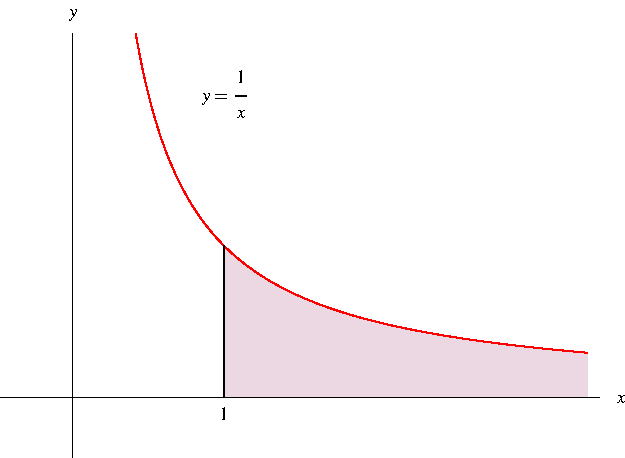
\includegraphics[height=3cm]{improper-integrals/pictures/08-08-ex1b.pdf}%

%\begin{center}
\uncover<7->{Infinite area}%
%\end{center}

\ \uncover<8->{%
\psset{xunit=1cm, yunit=1cm}
\begin{pspicture}(-0.4, -0.4)(3.3,2.2)
\tiny
\fcAxesStandard{-0.400000}{-0.4}{3.200000}{2}
\pscustom*[linecolor=cyan]{
%Function formula: x^{-2}

\psplot[linecolor=\fcColorGraph, plotpoints=1000]{1.000000}{3.000000}{x -2.0000000 exp }\psline(3.000000, 0)(1.000000, 0)}

%Function formula: x^{-2}

\psplot[linecolor=\fcColorGraph, plotpoints=1000]{0.75}{3.000000}{x -2.0000000 exp }
\rput(1.5, 1.5){$y=\frac{1}{x^2}$}

\end{pspicture}

%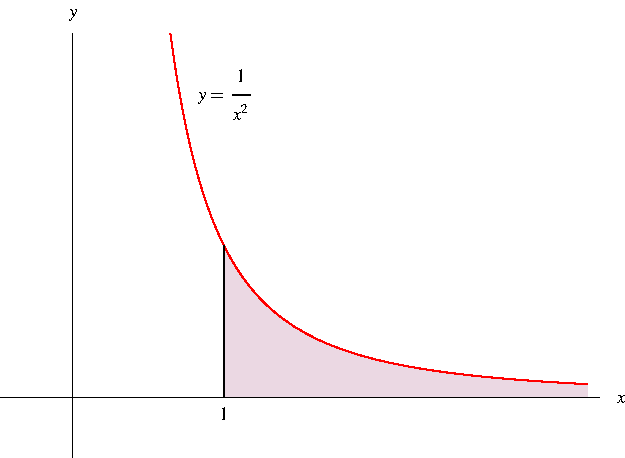
\includegraphics[height=3cm]{improper-integrals/pictures/08-08-ex1a.pdf}%
}%

%\begin{center}
\uncover<8->{Finite area}%
%\end{center}
\column{.6\textwidth}
\begin{eqnarray*}
\uncover<2->{%
\int_1^\infty \frac{1}{x}\diff x%
}%
& \uncover<2->{ = } & %
\uncover<2->{%
\lim_{t\rightarrow \infty} \int_1^t \frac{1}{x}\diff x%
}\\%
& \uncover<3->{ = } & %
\uncover<3->{%
\lim_{t\rightarrow \infty} \left[ \ln x\right]_1^t%
}\\%
& \uncover<4->{ = } & %
\uncover<4->{%
\lim_{t\rightarrow \infty} (\ln t - \ln 1)%
}\\%
& \uncover<5->{ = } & %
\uncover<5->{%
\lim_{t\rightarrow \infty} \ln t%
}%
\uncover<6->{ = \infty }%
\end{eqnarray*}
\uncover<7->{Therefore the improper integral is divergent.}
\end{columns}
\end{example}
\end{frame}
% end module improper-integral-type1-ex1


%% begin module improper-integral-type1-ex4
\begin{frame}
\begin{example} %[Example 4, p. 547]
For what values of $p$ is the integral $\int_1^\infty \frac{1}{x^p}\diff x$ convergent?
\begin{itemize}
\item<2->  We know from Example 1 that if $p = 1$, the integral is divergent.
\item<3->  Assume $p\neq 1$.
\end{itemize}
\abovedisplayskip=0pt
\belowdisplayskip=0pt
\[
\uncover<4->{%
\int_1^\infty \frac{1}{x^p} \diff x%
}%
 \uncover<4->{ = }  %
\uncover<4->{%
\lim_{t\rightarrow \infty}\int_1^t \frac{1}{x^p} \diff x%
}%
 \uncover<5->{ = }  %
\uncover<5->{%
\lim_{t\rightarrow \infty}\left[ \frac{x^{-p+1}}{-p+1}\right]_1^t%
}%
 \uncover<6->{ = }  %
\uncover<6->{%
\lim_{t\rightarrow \infty}\frac{ \frac{1}{t^{p-1}} - 1}{1-p}%
}%
\]
\begin{itemize}
\item<7->  If $p > 1$, then $p - 1 > 0$, so as $t\rightarrow \infty$, $t^{p-1}\rightarrow \infty$ and $1/t^{p-1}\rightarrow 0$.
\item<8->  Therefore $\int_1^\infty \frac{1}{x^p}\diff x = \frac{1}{p-1}$ if $p > 1$, and so the integral is convergent.
\item<9->  If $p < 1$, then $p - 1 < 0$, so $\frac{1}{t^{p-1}} = t^{1-p} \rightarrow \infty$ as $t\rightarrow \infty$.
\item<10->  Therefore $\int_1^\infty \frac{1}{x^p}\diff x$ is divergent if $p < 1$.
\end{itemize}
\end{example}
\uncover<11->{%
\begin{theorem}
$\int_1^\infty \frac{1}{x^p}\diff x$ converges if $p > 1$ and diverges if $p \leq 1$.
\end{theorem}
}%
\end{frame}
% end module improper-integral-type1-ex4


%% begin module improper-integral-type2
\begin{frame}
\frametitle{Type II: Discontinuous Integrands}
We can use the same approach if the function $f$ is discontinuous at one of the endpoints $a$ and $b$ in the integral $\int_a^b f(x) \diff x$.

For example, $\frac{1}{\sqrt{x - 2}}$ is discontinuous at $2$, so we might wonder if the integral
\[
\int_2^5 \frac{1}{\sqrt{x-2}}\diff x
\]
exists.

\begin{center}
\psset{xunit=1cm, yunit=1cm}
\begin{pspicture}(-0.5, -0.5)(5.600000,3.3)
\psframe*[linecolor=white](-0.5,-0.5)(5.600000,3.3)
\tiny
\pscustom*[linecolor=\fcColorAreaUnderGraph]{
%Function formula: \frac{1}{(x-2)^{1/2}}
\psplot[linecolor=\fcColorGraph, plotpoints=1000]{2.100000}{5.000000}{1.0000000 -2.0000000 x add 0.5000000 exp div }
\psline(5.000000, 0)(2.00000, 0)(2,3.16227766)
}
%Function formula: \frac{1}{(x-2)^{1/2}}
\psplot[linecolor=\fcColorGraph, plotpoints=1000]{2.100000}{5.000000}{1.0000000 -2.0000000 x add 0.5000000 exp div }

\psaxes[arrows=<->](0,0)(-0.500000,-0.5)(5.5,3.2)
\fcLabels{5.5}{3.2}
\end{pspicture}
%\ 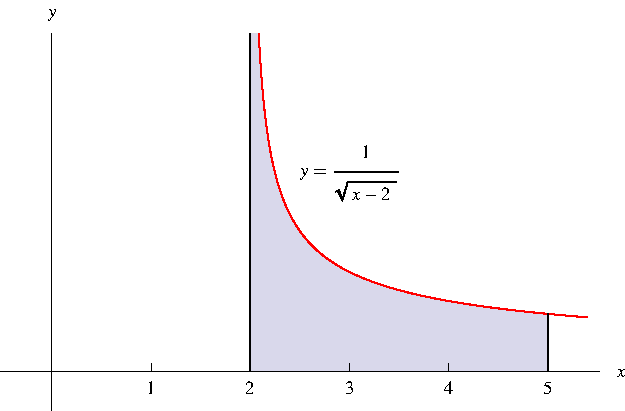
\includegraphics[height=3cm]{improper-integrals/pictures/08-08-ex5.pdf}%
\end{center}
\end{frame}

\begin{frame}
\begin{definition}[Improper Integral of Type II]
\begin{enumerate}
\item  If $f$ is continuous on $[a, b)$ and discontinuous at $b$, then
\abovedisplayskip=0pt
\belowdisplayskip=0pt
\[
\int_a^b f(x) \diff x = \lim_{t\rightarrow b^-} \int_a^t f(x) \diff x
\]
if the limit exists.
\item  If $f$ is continuous on $(a, b]$ and discontinuous at $a$, then
\abovedisplayskip=0pt
\belowdisplayskip=0pt
\[
\int_a^b f(x) \diff x = \lim_{t\rightarrow a^+} \int_t^b f(x) \diff x
\]
if the limit exists.
\end{enumerate}
$\int_a^bf(x) \diff x$ is called convergent if the corresponding limit exists and divergent if it doesn't exist.
\begin{enumerate}
\setcounter{enumi}{2}
\item  If $f$ has a discontinuity at $c$, where $a < c < b$, and both $\int_a^c f(x)\diff x$ and $\int_c^b f(x)\diff x$ are convergent, then we define
\abovedisplayskip=0pt
\belowdisplayskip=0pt
\[
\int_a^b f(x) \diff x = \int_a^c f(x)\diff x + \int_c^b f(x) \diff x
\]
\end{enumerate}
\end{definition}
\end{frame}
% end module improper-integral-type2


%% begin module trig-substitutions-ex3
\begin{frame}
\begin{example} %[Example 3, p. 505]
\begin{columns}[c]
\column{.4\textwidth}
Find $\int \frac{1}{x^2 \sqrt{x^2+4}}\diff x$.
\begin{itemize}
\item<2->  Let \alert<handout:0| 3-4,7,14,20>{$x = \uncover<4->{2\tan \theta}$}\uncover<4->{, where \alert<handout:0| 10>{$-\pi /2 \leq \theta \leq \pi / 2$}.}
\item<2->  Then \alert<handout:0| 5-6,13>{$\diff x = \uncover<6->{2\sec^2 \theta\diff \theta}$}\uncover<6->{.}
\end{itemize}
\column{.6\textwidth}
\begin{center}
\psset{xunit=2cm, yunit=2cm}
\begin{pspicture}(-0.15,-0.3)(2.3,1.2)
\psframe*[linecolor=white](-0.1,-0.3)(2.3,1.2)
\psline(0,0)(2, 0)(2,1)(0,0)
\psline(1.9,0)(1.9, 0.1)(2,0.1)
\fcAngle{0}{0.463648}{0.4}{$\theta$}
\uncover<handout:0|20->{
\rput[l](2.1, 0.5){$x$}
\rput[t](1, -0.1){$2$}
}
\uncover<handout:0|21->{
\rput[br](1, 0.55){$\sqrt{x^2+4}$}
}
%bounding box for pdflatex compilation:
\psline[linecolor=red!1](-0.11, -0.3 )(-0.105, -0.3)
\psline[linecolor=red!1](2.3, 1.21)(2.3, 1.205)
\end{pspicture}
%\ \only<handout:0| -19>{%
%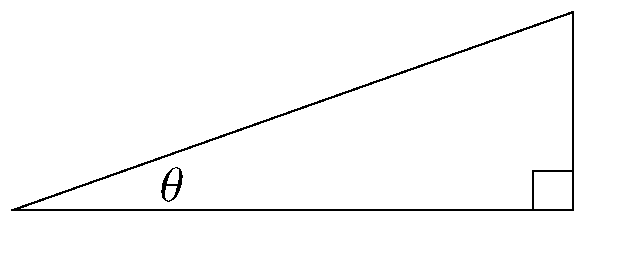
\includegraphics[height=3cm]{trig-substitution/pictures/08-03-ex3a.pdf}%
%}%
%\only<handout:0| 20>{%
%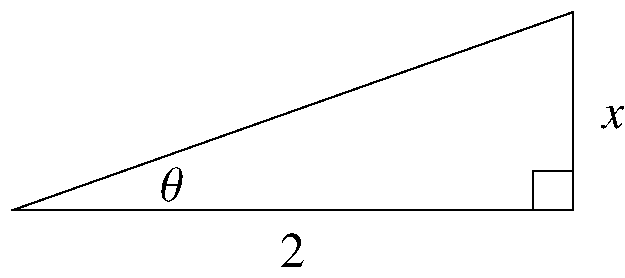
\includegraphics[height=3cm]{trig-substitution/pictures/08-03-ex3b.pdf}%
%}%
%\only<21->{%
%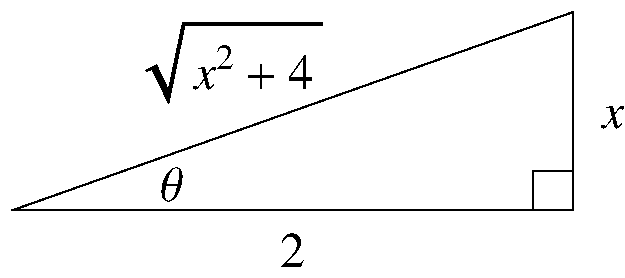
\includegraphics[height=3cm]{trig-substitution/pictures/08-03-ex3c.pdf}%
%}%
\end{center}
\end{columns}
\abovedisplayskip=0pt
\belowdisplayskip=0pt
\[
\uncover<2->{%
\alert<handout:0| 12>{%
\sqrt{\alert<handout:0| 7>{x^2} + 4} =
}%
}%
\uncover<7->{%
\sqrt{\alert<handout:0| 7>{4\tan^2 \theta} + 4} =
}%
\uncover<8->{%
\sqrt{4 \sec^2 \theta} =
}%
\uncover<9->{%
2 |\sec  \theta | =
}%
\uncover<10->{%
\alert<handout:0| 12>{%
2 \sec  \theta
}%
}%
\]
\abovedisplayskip=0pt
\belowdisplayskip=0pt
\begin{eqnarray*}
\uncover<11->{%
\int \frac{\alert<handout:0| 13>{\diff x}}{\alert<handout:0| 14>{x^2}\alert<handout:0| 12>{\sqrt{x^2+4}}}%
}%
& \uncover<11->{ = } & %
\uncover<11->{%
\int\frac{\alert<handout:0| 13>{2\sec^2 \theta \diff \theta}}{\alert<handout:0| 14>{4\tan^2 \theta}\cdot \alert<handout:0| 12>{2\sec \theta}}
}%
\uncover<15->{%
 = \frac{1}{4}\int \frac{\cos \theta}{\sin^2\theta} \diff \theta
}\\%
\uncover<16->{%
\textrm{Let } \alert<handout:0| 19>{u = \sin \theta} :%
}%
& \uncover<17->{ = } & %
\uncover<17->{%
\frac{1}{4} \int \frac{\diff u}{u^2}
}  \uncover<18->{ = }  \uncover<18->{%
\frac{1}{4} \left( -\alert<handout:0| 19>{\frac{1}{u}}\right)  + C
}\\%
& \uncover<19->{ = } & %
\uncover<19->{%
 -\frac{\alert<handout:0| 19,22-23>{\csc \theta}}{4} + C
}%
\uncover<23->{%
=  -\frac{\alert<handout:0| 23>{\sqrt{x^2+4}}}{4\alert<handout:0| 23>{x}} + C
}%
\end{eqnarray*}
\end{example}
\end{frame}
% end module trig-substitutions-ex3


%%begin module area-under-hyperbola-ex1

\begin{frame}
Recall Euler substitution: $x=\frac12\left(\frac{1}{t}- t \right)$, $\alert<2>{\sqrt{x^2+1}=\frac{1}2\left(\frac 1 t +t\right)}$, $\alert<12,13,14>{ t=\sqrt{x^2+1}-x} $, $\alert<3>{ \diff x=-\frac12 \left(\frac1{t^2} +1\right)\diff t}$.
\begin{example}
$
\begin{array}{rcl}
\displaystyle \int \alert<2>{ \sqrt{x^2+1}} \alert<3>{\diff x} \vphantom{ \frac{1}{8}\left(\frac{1}{ (\sqrt{ x^2 +1} -x)^2} - (\sqrt{x^2+1}- x)^2 \right) } &=&
\displaystyle
\only<1-16>{
\uncover<2->{ \alert<3>{-} \int  \alert<2>{\alert<4>{\frac12} \left(\alert<5,6>{\frac1t} +\alert<7,8>{t}\right)} \alert<3>{\alert<4>{ \frac{1}{2}} \left(\alert<5,7>{ \frac 1 {t^2}} +\alert<6,8>{1} \right)\diff t}} \\
\uncover<4->{ &=&\displaystyle -\alert<4>{ \frac 1 4} \alert<9,10,11>{ \int} \left(\alert<5>{ \alert<9>{ \frac{ 1 }{ t^3}}} + \alert<6,7,10>{2\frac{1}t} + \alert<8,11>{t} \right) \alert<9,10,11>{ \diff t} } \\
\uncover<9->{&=&\displaystyle \alert<15>{-\frac{1}4} \left( \alert<9>{ \alert<15>{ -}\frac{ \alert<12>{ t^{-2}}}{\alert<15>{2}}} +\alert<10>{ \alert<15>{2} \ln\alert<14>{ |t|} }+ \alert<11>{\frac{\alert<13>{ t^2}}{\alert<15>{2}}} \right)+C}\\
\uncover<12->{&=&}
}
\uncover<12->{\displaystyle \only<1-24>{  \alert<16,17,18,24>{ \alert<15>{\frac{1}{8}} \left(\frac{1}{\alert<12>{ (\sqrt{ x^2 +1} -x)^2}} - \alert<13>{\left(\sqrt{x^2+1}- x\right)^2} \right) } }}\only<25->{
\alert<25>{ \frac{1}{2}x\sqrt{x^2+1}}
} {~~~~~~~~~~~~~~~~~~~~~~~~~~~~~~~~~~~~~~~~~~~~~~~~~~~~~~}  \\
\uncover<12->{ && \displaystyle \alert<16,17>{ \only<1-30>{\alert<15>{ -}} \only<31->{\alert<31>{+} } \alert<15>{ \frac12}  \alert<26,30>{\ln \left( \alert<14>{ \sqrt{x^2+1} \only<1-30>{-}\only<31->{\alert<31>{+} } x} \right)} +C}}
\end{array}
$

\noindent \only<17-25>{The answer is good. However, let's simplify.

\noindent
\uncover<18->{
$
\begin{array}{l}
\phantom{=}
\displaystyle \alert<18>{ \frac{1}{(\sqrt{x^2+1}-x)^2}- \left( \sqrt{ x^2+1 }-x\right)^2} \\
\uncover<19->{= \displaystyle \frac{ \alert<19>{(\sqrt{x^2+1} +x )^2} }{ ( \sqrt{x^2 +1} -x )^2  	\alert<19>{(\sqrt{x^2+1}+x)^2} } - \left(\sqrt{x^2+1}-x\right)^2} \\
\uncover<20->{ =\displaystyle \frac{(\sqrt{x^2+1}+x)^2}{ \alert<20>{ \alert<21,22>{((\sqrt{x^2 +1 } )^2 -x^2 )^2 } \uncover<21,22>{\alert<21,22>{=1}} } } - \left( \sqrt{x^2 +1 } -x \right)^2} \\
\displaystyle \uncover<22->{=\left(\sqrt{x^2+1}+x\right)^2-\left( \sqrt{ x^2 + 1 } -x\right)^2} \uncover<23->{ = \alert<24,25>{ 4x\sqrt{x^2+1}}}
\end{array}
$
} %uncover<18->
} %only<17-25>

\only<26->{
The last expression can be transformed to:
\[
\begin{array}{rcl}
\displaystyle
\alert<26>{\ln} \left(\frac{\alert<26,28>{\left(\sqrt{x^2+1}-x\right)} \uncover<27->{ \alert<27,28>{\left( \sqrt{x^2+1}+ x \right)} }}{ \uncover<27->{ \alert<27>{ \sqrt{x^2 +1} +x}}} \right)
&=& \displaystyle \uncover<28->{\alert<29>{ \ln \left( \frac{\alert<28>{ 1} }{ \sqrt{x^2+1}+x}\right)} }\\ \uncover<29->{&=&\alert<29,30,31>{ -\ln \left(\sqrt{x^2+1}+x\right)}}
\end{array}
\]
}
\end{example}

\vspace{8cm}
\end{frame}

\begin{frame}
\begin{example}
Find the area locked b-n the hyperbolas $\alert<2,3>{ y=\pm \sqrt{ x^2+1}}$ and $x=\pm 2\sqrt{ 2}$.
\begin{columns}
\column{.5\textwidth}
\psset{xunit=0.7cm, yunit=0.7cm}
\begin{pspicture}(-3.328427, -3)(3.328427,3)
\psframe*[linecolor=white](-3.328427,-3)(3.328427,3)
\tiny
\uncover<31->{
\pscustom*[linecolor=\fcColorAreaUnderGraph]{
\psplot[linecolor=\fcColorGraph, plotpoints = 1000 ] {-2.828427} {2.828427}{1 x 2 exp add 0.5 exp }
\psline[linecolor=\fcColorGraph](2.828427,-3)(2.828427,3)
\psplot[linecolor=\fcColorGraph, plotpoints=1000] { 2.828427 } {-2.828427}{1 x 2 exp add 0.5 exp -1 mul }
\psline[linecolor=\fcColorGraph](-2.828427,-3)(-2.828427,3)
}
}
\uncover<1-26,28->{
\psaxes[arrows=<->,ticks=none, labels=none](0,0)(-3,-3)(3,3)
}
\psline[linecolor=red!1](3.301,2)(3.302,2)
\psline[linecolor=red!1](-3.301,2)(-3.302,2)

%Function formula: - (x^{2}+1)^{1/2}
\psplot[linecolor=\fcColorGraph, plotpoints=1000]{-2.828427}{2.828427}{1 x 2 exp add 0.5 exp -1 mul }
\uncover<3-4>{\rput[tl](-2.2, -2.4){ \alert<3>{ $y= - \sqrt{ x^2 +1 }$}}}

%Function formula: (x^{2}+1)^{1/2}
\psplot[linecolor=\fcColorGraph, plotpoints=1000]{-2.828427}{ 2.828427 }{1 x 2 exp add 0.5 exp }
\uncover<2-4>{\rput[bl](-2.1, 2.4){\alert<2>{ $y=\sqrt{ x^2 +1} $}}}

\uncover<29->{
\psline[linecolor=\fcColorGraph](-2.828427,3)(-2.828427,-3)
}
\uncover<30->{
\psline[linecolor=\fcColorGraph](2.828427,3)(2.828427,-3)
}
\uncover<25-27>{
\psline{<->}(-2.9,2.9)(2.9,-2.9)
\rput[t](-2.1, 1.7){$\begin{array}{l} \alert<25>{v=0} \\\uncover<1-26>{\alert<25>{y+x=0}} \end{array}$}
}
\uncover<15-27>{
\psline{<->}(-2.9,-2.9)(2.9,2.9)
\rput[b](-2.1, -1.9){$\begin{array}{l} \uncover<1-26>{ \alert<15>{ y-x=0 }}\\\uncover<16->{\alert<16>{u=0}} \end{array}$}
}
\uncover<17-26>{
\fcFullDot{1.4}{1.4}
\rput[l]( 1.6, 1.4){$(\frac{y+x}{2},\frac{y+x}{2})$}
}
\uncover<14-26>{
\fcFullDot{0.6}{2.2}
\rput[lb](0.65, 2.2){$(x,y)$}
}
\uncover<26>{
\psline(0.6,2.2)(-0.8,0.8)
\psline(-0.7, 0.9)(-0.6, 0.8)(-0.7, 0.7)
\rput[rb](-0.3, 1.3){\alert<26>{$v$}}
}
\uncover<18-26>{
\psline(0.6,2.2)(1.4, 1.4)
\psline(1.3, 1.5)(1.2,1.4)(1.3, 1.3)
}
\uncover<23-26>{
\rput[tr](0.95, 1.8){\alert<23>{$u$}}
}
\uncover<14-26>{
\fcFullDot{2.2}{0.6}
\rput[lt]( 2.2, 0.65){$(y,x)$}
}
\end{pspicture}

\vbox to 3.0cm {
\uncover<18->{\alert<18>{
\uncover<22->{\alert<22>{Signed}} distance b-n $(x,y)$ and line $u=0$ equals}}
\only<1-23>{
$\uncover<19->{\uncover<22->{\alert<22>{\pm}} \alert<19>{ \sqrt{ \alert<20>{ \left(x-\frac{(x+y)}{2} \right)^2+ \left( y- \frac{(x+y )}{2} \right)^2}}}}
$
$\uncover<20->{=\uncover<22->{\alert<22>{\pm}} \sqrt{ \alert<20>{ \frac{1}{2}(y-x)^2 }}} \uncover<21->{= \alert<21>{ \uncover<1-21>{\pm} \alert<23>{ \frac{\sqrt{2 }}{ 2 } ( y-x)}}} \uncover<23>{ \alert<23>{=}}$
} %only<1-23>
\uncover<23->{ \alert<23,24>{$u $}.}
\only<24->{\uncover<25->{
Similarly compute that \alert<26>{signed distance b-n $(x,y)$ and the \alert<25>{line $v=0$} equals $v$}.
\uncover<27->{$\Rightarrow$ $y^2-x^2=1$ is the \alert<27>{ hyperbola $v=\frac{1/2}{v}$} in the $(u,v)$-plane.}
}}

\vfil
} %vbox

\column {.5\textwidth}
\only<1-27>{
\uncover<4->{We studied $\alert<27>{v=\frac{1/2}{u}}$ is called a hyperbola:}\uncover<3->{ why do we call $y= \sqrt{ x^2 +1}$ hyperbola?} \uncover<5->{Compute:}
\[
\begin{array}{rcl}
\uncover<5->{\sqrt{x^2+1} &=& y}\\
\uncover<6->{ x^2+1 &=& y^2}\\
\uncover<7->{y^2-x^2&=&1}\\
\uncover<8->{\uncover<9>{\alert<9>{\frac{1}{2}}} \uncover<10->{\alert<10,11>{\frac{\sqrt{2}}{2}}} \alert<11>{(y-x)} \uncover<10->{\alert<10,12>{\frac{\sqrt{2}}{2}}} \alert<12>{(y+x)}&=&\uncover<9->{\alert<9>{\frac{1}{2}}} \uncover<8>{1}}\\
\uncover<11->{\alert<11>{u}\alert<12>{v}&=& \frac{1}{2}}\\
\uncover<13->{\alert<27>{v}&\alert<27>{=}& \alert<27>{\frac{1/2}{u}},}
\end{array}
\]
\uncover<11->{where $\begin{array}{|l}
\alert<11,16,23>{u=\frac{\sqrt{2}}{2} \left(y-x\right)}\\
\alert<12,25>{v=\frac{\sqrt{2}}{2}\left(y+x\right)}
\end{array}$. } \uncover<14->{Consider an arbitrary point $(x,y)$.}
} %only<1-27>
\only<28->{
The area in question is:
$
\begin{array}{l}
\displaystyle\phantom{=} \int \limits^{{{\uncover<28,29>{\alert<29>{ \textbf{?}}}\uncover<30->{\alert<30>{ 2\sqrt{2}}}}}}_{\uncover<28>{\alert<28>{\textbf{?}}}\uncover<29->{ -2\sqrt{2}}} 2\sqrt{x^2+1}\diff x \\
\displaystyle \uncover<32->{= \uncover<33->{\alert<33>{2}} \left[x\sqrt{x^2+1} \vphantom{\ln \left(\sqrt{x^2+1}+x\right) }\right.}\\
\displaystyle \uncover<32->{\left. \ln \left(\sqrt{x^2+1}+x\right)\right]^{2\sqrt{2}}_{\only<33->{\alert<33>{0}} \uncover<1-32>{-2\sqrt{2}}}}\\
\uncover<34->{=2\left(2\sqrt{2} \sqrt{(2\sqrt{2})^2+1}\right.} \\
\uncover<34->{\left.+ \ln \left(\sqrt{(2\sqrt{2})^2+1}+2\sqrt{2} \right) \right)}\\
\uncover<35->{=12\sqrt{2} +2\ln \left(3+2\sqrt{2}\right )}\\
\uncover<36->{\approx 20.496}
\end{array}
$
}
\end{columns}

\end{example}

\end{frame}

%end module area-under-hyperbola-ex1


%%begin module quadratic-radicals-linear-substitution-preparation-ex1
\begin{frame}
\frametitle{Linear substitutions to simplify radicals $\sqrt{ay^2+by+c}$}
\begin{itemize}
\item Using linear substitutions, radicals of form  $\sqrt{ay^2+by+c}$, $a\neq 0$, $b^2-4ac\neq 0$ can be transformed to (multiple of):
\begin{itemize}
\item $\sqrt{x^2+1}$ 
\item $\sqrt{-x^2+1}$
\item $\sqrt{x^2-1}$.
\end{itemize}
\item We already studied how to do that using completing the square when dealing with rational functions. 
\end{itemize}
\end{frame}
\begin{frame}
Recall: linear substitution is subst. of the form $u=px+q$.
\begin{example}
Use linear substitution to transform $\sqrt{x^2+x+1}$ to multiple of $\sqrt{u^2+1}$. 

\noindent $
\begin{array}{rcl}
\sqrt{x^2+x+1}&=&\displaystyle \uncover<2->{ \sqrt{ x^2+2\frac{1}{2}x + \uncover<3->{ \alert<3>{ \frac{1}{4} } } \uncover<2>{ \alert<2>{ \textbf{?}}} \uncover<2->{ \alert<2,3>{-} } \uncover<3->{ \alert<3>{ \frac{1}{4}}} \uncover<2>{\alert<2>{\textbf{?}}} +1}} \\
\uncover<4->{&=&\displaystyle \sqrt{ {\left(x+\uncover<5->{\alert<5>{\frac{1}{2}}} \uncover<4>{ \alert<4>{ \textbf{?}}} \right)}^2- \uncover<4>{\alert<4>{\textbf{?} }} \uncover<5->{ \alert<5,6>{ \frac{3}{4}}} }} \\
\uncover<6->{&=&\displaystyle \sqrt{ \alert<6,7>{ \frac{3}{4}}\left( \alert<6,8>{\frac{4}{3}} \left(x+\frac{1}{2}\right)^{\alert<8>{2}} +\alert<6>{ 1} \right)}}\\
\uncover<7->{&=&\displaystyle \alert<7>{\frac{\sqrt{3}}{2}} \sqrt{\left(  \alert<9>{\alert<8>{\frac{2}{\sqrt{3}}} \left( x+ \frac{1}{2} \right)}\right)^{\alert<8>{2}}+1}}\\
\uncover<9->{ &=&\displaystyle \frac{\sqrt{3}}{2} \sqrt{ {\alert<9>{u}}^2+1},}
\end{array}
$

\noindent \uncover<9->{ where $\displaystyle \alert<9>{u= \frac{2}{\sqrt{3}}\left( x+\frac{1}{2}\right)}  =\frac{2\sqrt{3}}{3}x +\frac{\sqrt{3}}{3} $.}
\end{example}
\vspace{5cm}
\end{frame}
%end module quadratic-radicals-linear-substitution-preparation-ex1
%%begin module partial-fractions-building-blocks-2a-and-3a
%This module may be too long, perhaps a split is needed.


%\begin{comment}






%\end{comment}
%end module partial-fractions-building-blocks-2a-and-3a
%% begin module orthogonal-trajectory-ex5
\begin{frame}
\begin{example}
Find the orthogonal trajectories of the family $x = ky^2$, where $k$ is an arbitrary constant.  \uncover<3->{\alert<handout:0| 3>{Differentiate implicitly:}}
\begin{columns}[c]
\column{.5\textwidth}
\abovedisplayskip=0pt
\belowdisplayskip=0pt
\begin{eqnarray*}
\uncover<2->{%
\alert<handout:0| 5>{x}%
}%
& \uncover<2->{ \alert<handout:0| 5>{=} } &%
\uncover<2->{%
\alert<handout:0| 5>{ky^2}%
}\\%
\uncover<3->{%
1%
}%
& \uncover<3->{ = } &%
\uncover<3->{%
2\alert<handout:0| 4-5>{k}y\frac{\diff y}{\diff x}%
}\\%
\uncover<4->{%
1%
}%
& \uncover<4->{ = } &%
\uncover<4->{%
2\left(\alert<handout:0| 4-5>{\uncover<5->{\frac{x}{y^2}}}\right) y\frac{\diff y}{\diff x}%
}\\%
\uncover<6->{%
\frac{\diff y}{\diff x}%
}%
& \uncover<6->{ = } &%
\uncover<6->{%
\frac{y}{2x}%
}%
\end{eqnarray*}
%\begin{center}

\hfil\hfil\psset{xunit=0.4cm, yunit=0.4cm}
\begin{pspicture}(-4.4, -3.228427)(4.4,3.317125)
\tiny
\fcAxesStandard{-4.15}{-2.978427}{4.15}{2.967125}
%Calculator input: plotCurve{}(1/2 t^{2}, t, - (8)^{1/2}, (8)^{1/2})
\parametricplot[linecolor=\fcColorGraph, plotpoints=1000]{-2.82843}{2.82843}{t 2 exp 0.5 mul t}
%Calculator input: plotCurve{}(-1/2 t^{2}, t, - (8)^{1/2}, (8)^{1/2})
\parametricplot[linecolor=\fcColorGraph, plotpoints=1000]{-2.82843}{2.82843}{t 2 exp -0.5 mul t}
%Calculator input: plotCurve{}(t^{2}, t, - (4)^{1/2}, (4)^{1/2})
\parametricplot[linecolor=\fcColorGraph, plotpoints=1000]{-2}{2}{t 2 exp t}
%Calculator input: plotCurve{}(- t^{2}, t, - (4)^{1/2}, (4)^{1/2})
\parametricplot[linecolor=\fcColorGraph, plotpoints=1000]{-2}{2}{t 2 exp -1 mul t}
%Calculator input: plotCurve{}(-2 t^{2}, t, - (2)^{1/2}, (2)^{1/2})
\parametricplot[linecolor=\fcColorGraph, plotpoints=1000]{-1.41421}{1.41421}{t 2 exp -2 mul t}
%Calculator input: plotCurve{}(2 t^{2}, t, - (2)^{1/2}, (2)^{1/2})
\parametricplot[linecolor=\fcColorGraph, plotpoints=1000]{-1.41421}{1.41421}{t 2 exp 2 mul t}
\uncover<11->{%
%Calculator input: plotCurve{}(1/2 \cos{}t, 1/2\sqrt{2} \sin{}t, 0, 2 \pi)
\parametricplot[linecolor=blue, plotpoints=1000]{0}{6.28319}{t 57.29578 mul cos 0.5 mul t 57.29578 mul sin 0.707107 mul }%
%Calculator input: plotCurve{}(3/2 \cos{}t, 3/2\sqrt{2} \sin{}t, 0, 2 \pi)
\parametricplot[linecolor=blue, plotpoints=1000]{0}{6.28319}{t 57.29578 mul cos 1.5 mul t 57.29578 mul sin 2.12132 mul }%
%Calculator input: plotCurve{}(\cos{}t, \sqrt{2} \sin{}t, 0, 2 \pi)
\parametricplot[linecolor=blue, plotpoints=1000]{0}{6.28319}{t 57.29578 mul cos t 57.29578 mul sin 1.414214 mul }%
}%
%\fcFullDot{1.081139}{1.470469}
\end{pspicture}

%\end{center}
\column{.5\textwidth}
\uncover<7->{%
An orthogonal trajectory will have a slope that is the negative reciprocal of the slope of the curve.
}%
\abovedisplayskip=0pt
\belowdisplayskip=0pt
\begin{eqnarray*}
\uncover<7->{%
\frac{\diff y}{\diff x}%
}%
& \uncover<7->{ = } &%
\uncover<7->{%
-\frac{2x}{y}%
}\\%
\uncover<8->{%
\int y \diff y%
}%
& \uncover<8->{ = } &%
\uncover<8->{%
-\int 2x\diff x%
}\\%
\uncover<9->{%
\frac{y^2}2%
}%
& \uncover<9->{ = } &%
\uncover<9->{%
-x^2 + C%
}\\%
\uncover<10->{%
x^2 + \frac{y^2}{2} %
}%
& \uncover<10->{ = } &%
\uncover<10->{%
C%
}%
\end{eqnarray*}
\uncover<11->{%
The ellipses $x^2 + \frac{y^2}{2} = C$ are all orthogonal trajectories to $x = ky^2$.
}%
\end{columns}
\end{example}
\end{frame}
% end module orthogonal-trajectory-ex5


%%begin module polar-two-points-coincide-iff
\begin{frame}
\begin{itemize}
\item Let $P_1$ be point  with polar coordinates $(r_1, \theta_1)$.
\item Let $P_2$ be point  with polar coordinates $(r_2, \theta_2)$.
\end{itemize}

\uncover<2->{
\begin{observation}
$P_1$ coincides with $P_2$ if one of the three mutually exclusive possibilities holds:
\begin{itemize}
\item<alert@3> $r_1=r_2\neq 0$ and $\theta_2=\theta_1+2k\pi, k\in \mathbb Z $,
\item<alert@4> $r_1=-r_2\neq 0$ and $\theta_2=\theta_1+(2k+1)\pi, k\in \mathbb Z$,
\item $r_1=r_2=0 $ and $\theta$ is arbitrary.
\end{itemize}
\end{observation}
}
\begin{columns}
\column{.5\textwidth}
\only<3>{
\psset{xunit=2cm, yunit=2cm}
\begin{pspicture}(-0.9, -1.1)(2,0.75) 
\tiny 
%force a boudning box:
%\psline[linecolor=red!1](-0.1, -0.1)(-0.21,0.2)
%\psline[linecolor=red!1](1.1, 0.6)(1.1,0.61)
\psFullDotBlue{0}{0}

%Calculator input: plotCurve{}(1/10 \cos{}t, 1/10 \sin{}t, 0, -3/4 \pi)
\parametricplot[arrows=->, linecolor=\psColorGraph, plotpoints=100]{0} {3.926990817} {t 57.29578 mul cos 0.3000000 mul t 57.29578 mul sin 0.3000000 mul }
\rput[t] (0,-0.1){$O$}
\rput[l](0.3, 0.3){$\theta_1$}

\psline{->}(0,0)(2,0)
\psline[linecolor=blue](0,0)(-0.707106781, -0.707106781)
\psFullDotBlue{-0.707106781}{-0.707106781}
\rput[tl](-0.6, -0.7){$(r_1,\theta_1)$}
\end{pspicture} 
}
\uncover<4>{
\psset{xunit=2cm, yunit=2cm}
\begin{pspicture}(-0.9, -1.1)(2,0.75) 
\tiny 
%force a boudning box:
%\psline[linecolor=red!1](-0.1, -0.1)(-0.21,0.2)
\psline[linecolor=red!1](1.1, 0.5)(1.1,0.51)
\psFullDotBlue{0}{0}

%Calculator input: plotCurve{}(1/10 \cos{}t, 1/10 \sin{}t, 0, -3/4 \pi)
\parametricplot[arrows=->, linecolor=\psColorGraph, plotpoints=100]{0} {-2.35619} {t 57.29578 mul cos 0.3000000 mul t 57.29578 mul sin 0.3000000 mul }
\rput[t] (0,-0.1){$O$}
\rput[l](0.3, -0.2){$\theta_1$}

\psline{->}(0,0)(2,0)
\psline[linecolor=blue](0,0)(-0.707106781, -0.707106781)
\psFullDotBlue{-0.707106781}{-0.707106781}
\rput[tl](-0.6, -0.7){$(r_1,\theta_1)$}
\end{pspicture} 
}

%\ \uncover<1->{%
%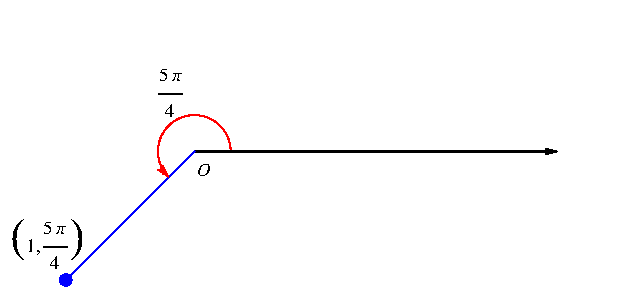
\includegraphics[height=3cm]{polar-curves/pictures/11-03-ex1a.pdf}%
%}%

%\ \uncover<2->{%
%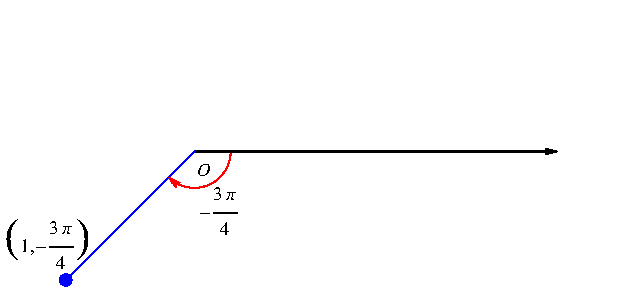
\includegraphics[height=3cm]{polar-curves/pictures/11-03-ex1b.pdf}%
%}%

\vspace{2cm}
\column{.5\textwidth}
\only<3>{
\psset{xunit=2cm, yunit=2cm}
\begin{pspicture}(-0.9, -1.1)(2,0.75) 
\tiny 
%force a boudning box:
%\psline[linecolor=red!1](-0.1, -0.1)(-0.21,0.2)
%\psline[linecolor=red!1](1.1, 0.6)(1.1,0.61)
\psFullDotBlue{0}{0}

%Calculator input: plotCurve{}(1/50 t \cos{}t+3/20 \cos{}t, 1/50 t \sin{}t+3/20 \sin{}t, 0, 13/4 \pi)
\parametricplot[arrows=->, linecolor=\psColorGraph, plotpoints=400] {0} {10.2102} {t 57.29578 mul cos 0.1500000 mul t 57.29578 mul cos t mul 0.0200000 mul add t 57.29578 mul sin 0.1500000 mul t 57.29578 mul sin t mul 0.0200000 mul add }

\rput[t] (0,-0.1){$O$}
\rput[l](0.3, 0.3){$\theta_2=\theta_1+2\pi$}

\psline{->}(0,0)(2,0)
\psline[linecolor=blue](0,0)(-0.707106781, -0.707106781)
\psFullDotBlue{-0.707106781}{-0.707106781}
\rput[tl](-0.6, -0.7){$(r_2, \theta_2)=(r_1,\theta_1+2\pi)$}
\end{pspicture} 
}

\uncover<4>{
\psset{xunit=2cm, yunit=2cm}
\begin{pspicture}(-0.9, -1.1)(2,0.75) 
\tiny 
%force a boudning box:
%\psline[linecolor=red!1](-0.1, -0.1)(-0.21,0.2)
\psline[linecolor=red!1](1.1, 0.5)(1.1,0.51)
\psFullDotBlue{0}{0}

%Calculator input: plotCurve{}(1/10 \cos{}t, 1/10 \sin{}t, 0, -3/4 \pi)
\parametricplot[arrows=->, linecolor=\psColorGraph, plotpoints=100]{0} {0.785398163} {t 57.29578 mul cos 0.3000000 mul t 57.29578 mul sin 0.3000000 mul }
\rput[t] (0,-0.1){$O$}
\rput[l](0.35, 0.15){$\theta_2=\theta_1+\pi$}

\psline{->}(0,0)(2,0)
\psline[linecolor=blue](0,0)(-0.707106781, -0.707106781)
\psFullDotBlue{-0.707106781}{-0.707106781}
\psline[linestyle=dashed](0,0)(0.707106781, 0.707106781)
\psFullDotBlack{0.707106781}{0.707106781}
\rput[tl](-0.6, -0.7){$(r_2, \theta_2)=(-r_1,\theta_1+\pi)$}
\end{pspicture} 
}
%\ \uncover<3->{%
%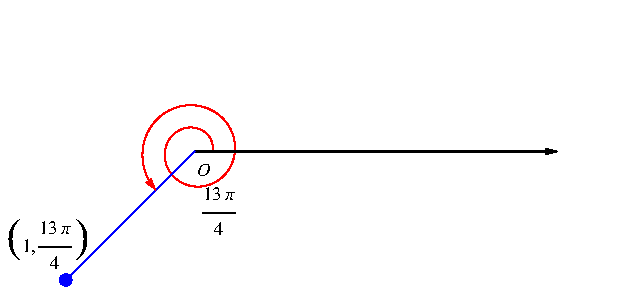
\includegraphics[height=3cm]{polar-curves/pictures/11-03-ex1c.pdf}%
%}%

%\ \uncover<4->{%
%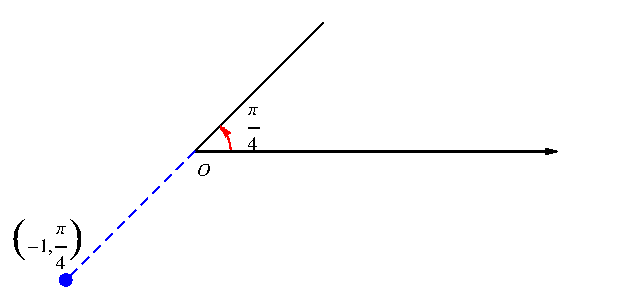
\includegraphics[height=3cm]{polar-curves/pictures/11-03-ex1d.pdf}%
%}%

\vspace{2cm}
\end{columns}
\end{frame}
%end module polar-two-points-coincide-iff


%% begin module cycloid-def
\begin{frame}
\frametitle{The Cycloid}

\psset{xunit=0.8cm, yunit=0.8cm}
\begin{pspicture}(-1.499950, -0.5)(14.066321,5)
\psframe*[linecolor=white](-1.499950,-0.1)(14.066321,5)
\tiny

%circles generated by calculator commands:
%precision:=0.99995;f{}{{t}}:=plot2D(\sqrt{1-(x-t)^2}+1, t-precision, t+precision )+plot2D(-\sqrt{1-(x-t)^2}+1, t-precision, t+precision );f{}(0)+f{}(0.5\pi)+f{}(\pi)+f{}(1.5\pi)+f{}(2\pi)+f{}(2.5\pi)+f{}(3\pi)+f{}(3.5\pi)+f{}(4\pi)

\fcAxesStandard{-1.1}{-0.5}{13.566321}{2.3}

%calcululator commands: f{}{{t}}:=(DoubleValue (t\pi-sin (t\pi) ), 1-cos (\pi t));(f{}0, f{}0.5, f{}1, f{}1.5, f{}2, f{}2.5, f{}3, f{}3.5, f{}4)
%generate the following points:
%(0.000000, 0.000000), (0.570796, 1.000000), (3.141593, 2), (5.712389, 1.000000), (6.283185, 0.000000), (6.853982, 1.000000), (9.424778, 2.000000), (11.995574, 1.000000), (12.566371, 0.000000)

\uncover<1>{
%Function formula: (- x^{2}+1)^{1/2}+1
\psplot[linecolor=\fcColorTangent, plotpoints=1000]{-0.999990}{0.999990}{1.0000000 1.0000000 x 2.0000000 exp -1.0000000 mul add 0.5000000 exp add }
%Function formula: - (- x^{2}+1)^{1/2}+1
\psplot[linecolor=\fcColorTangent, plotpoints=1000]{-0.999990}{0.999990}{1.0000000 1.0000000 x 2.0000000 exp -1.0000000 mul add 0.5000000 exp -1.0000000 mul add }
\fcFullDot{0}{0}
\rput[bl](0.1, 0.1){$P$}
}

\uncover<2>{
%Function formula: (- (x-1/2 \pi)^{2}+1)^{1/2}+1
\psplot[linecolor=\fcColorTangent, plotpoints=1000]{0.570806}{2.570786}{1.0000000 1.0000000 3.141592654 -0.5000000 mul x add 2.0000000 exp -1.0000000 mul add 0.5000000 exp add }
%Function formula: - (- (x-1/2 \pi)^{2}+1)^{1/2}+1
\psplot[linecolor=\fcColorTangent, plotpoints=1000]{0.570806}{2.570786}{1.0000000 1.0000000 3.141592654 -0.5000000 mul x add 2.0000000 exp -1.0000000 mul add 0.5000000 exp -1.0000000 mul add }
\fcFullDot{0.570796}{1}
\rput[l](0.670796, 1.000000){$P$}
}

\uncover<3>{
%Function formula: (- (x- \pi)^{2}+1)^{1/2}+1
\psplot[linecolor=\fcColorTangent, plotpoints=1000]{2.141603}{4.141583}{1.0000000 1.0000000 3.141592654 -1.0000000 mul x add 2.0000000 exp -1.0000000 mul add 0.5000000 exp add }
%Function formula: - (- (x- \pi)^{2}+1)^{1/2}+1
\psplot[linecolor=\fcColorTangent, plotpoints=1000]{2.141603}{4.141583}{1.0000000 1.0000000 3.141592654 -1.0000000 mul x add 2.0000000 exp -1.0000000 mul add 0.5000000 exp -1.0000000 mul add }
\fcFullDot{3.141593}{2}
\rput[t](3.141593, 1.9){$P$}
}

\uncover<4>{
%Function formula: (- (x-3/2 \pi)^{2}+1)^{1/2}+1
\psplot[linecolor=\fcColorTangent, plotpoints=1000]{3.712399}{5.712379}{1.0000000 1.0000000 3.141592654 -1.5000000 mul x add 2.0000000 exp -1.0000000 mul add 0.5000000 exp add }
%Function formula: - (- (x-3/2 \pi)^{2}+1)^{1/2}+1
\psplot[linecolor=\fcColorTangent, plotpoints=1000]{3.712399}{5.712379}{1.0000000 1.0000000 3.141592654 -1.5000000 mul x add 2.0000000 exp -1.0000000 mul add 0.5000000 exp -1.0000000 mul add }
\fcFullDot{5.712389}{1}
\rput[r](5.612389, 1){$P$}
}

\uncover<5>{
%Function formula: - (- (x-2 \pi)^{2}+1)^{1/2}+1
\psplot[linecolor=\fcColorTangent, plotpoints=1000]{5.283195}{7.283175}{1.0000000 1.0000000 3.141592654 -2.0000000 mul x add 2.0000000 exp -1.0000000 mul add 0.5000000 exp -1.0000000 mul add }
%Function formula: (- (x-2 \pi)^{2}+1)^{1/2}+1
\psplot[linecolor=\fcColorTangent, plotpoints=1000]{5.283195}{7.283175}{1.0000000 1.0000000 3.141592654 -2.0000000 mul x add 2.0000000 exp -1.0000000 mul add 0.5000000 exp add }
\fcFullDot{6.283185}{0}
\rput[lb](6.283185, 0.1){$P$}
}

\uncover<6>{
%Function formula: (- (x-5/2 \pi)^{2}+1)^{1/2}+1
\psplot[linecolor=\fcColorTangent, plotpoints=1000]{6.853992}{8.853972}{1.0000000 1.0000000 3.141592654 -2.5000000 mul x add 2.0000000 exp -1.0000000 mul add 0.5000000 exp add }
%Function formula: - (- (x-5/2 \pi)^{2}+1)^{1/2}+1
\psplot[linecolor=\fcColorTangent, plotpoints=1000]{6.853992}{8.853972}{1.0000000 1.0000000 3.141592654 -2.5000000 mul x add 2.0000000 exp -1.0000000 mul add 0.5000000 exp -1.0000000 mul add }
\fcFullDot{6.853982}{1}
\rput[l](6.953982, 1.000000){$P$}
}

\uncover<7>{
%Function formula: (- (x-3 \pi)^{2}+1)^{1/2}+1
\psplot[linecolor=\fcColorTangent, plotpoints=1000]{8.424788}{10.424768}{1.0000000 1.0000000 3.141592654 -3.0000000 mul x add 2.0000000 exp -1.0000000 mul add 0.5000000 exp add }
%Function formula: - (- (x-3 \pi)^{2}+1)^{1/2}+1
\psplot[linecolor=\fcColorTangent, plotpoints=1000]{8.424788}{10.424768}{1.0000000 1.0000000 3.141592654 -3.0000000 mul x add 2.0000000 exp -1.0000000 mul add 0.5000000 exp -1.0000000 mul add }
\fcFullDot{9.424778}{2}
\rput[t](9.424778, 1.9){$P$}
}

\uncover<8>{
%Function formula: - (- (x-7/2 \pi)^{2}+1)^{1/2}+1
\psplot[linecolor=\fcColorTangent, plotpoints=1000]{9.995584}{11.995564}{1.0000000 1.0000000 3.141592654 -3.5000000 mul x add 2.0000000 exp -1.0000000 mul add 0.5000000 exp -1.0000000 mul add }
%Function formula: (- (x-7/2 \pi)^{2}+1)^{1/2}+1
\psplot[linecolor=\fcColorTangent, plotpoints=1000]{9.995584}{11.995564}{1.0000000 1.0000000 3.141592654 -3.5000000 mul x add 2.0000000 exp -1.0000000 mul add 0.5000000 exp add }
\fcFullDot{11.995574}{1}
\rput[r](11.895574, 1.000000){$P$}
}

\uncover<9>{
%Function formula: (- (x-4 \pi)^{2}+1)^{1/2}+1
\psplot[linecolor=\fcColorTangent, plotpoints=1000]{11.566381}{13.566361}{1.0000000 1.0000000 3.141592654 -4.0000000 mul x add 2.0000000 exp -1.0000000 mul add 0.5000000 exp add }
%Function formula: - (- (x-4 \pi)^{2}+1)^{1/2}+1
\psplot[linecolor=\fcColorTangent, plotpoints=1000]{11.566381}{13.566361}{1.0000000 1.0000000 3.141592654 -4.0000000 mul x add 2.0000000 exp -1.0000000 mul add 0.5000000 exp -1.0000000 mul add }
\fcFullDot{12.566371}{0}
\rput[lb](12.566371, 0.1){$P$}
}

%Calculator input:f{}{{p}}:=plotCurve(t+\cos(- t+3\pi/2), 1+\sin(3\pi/2- t),p, p+\pi/4)+ plotCurve(t+\cos(- t+3\pi/2), 1+\sin(3\pi/2- t), p+\pi/4, p+\pi/2); f{}0+f{}(0.5\pi)+ f{}(\pi)+f{}(1.5\pi)+f{}(2\pi)+f{}(2.5\pi)+f{}(3\pi)+f{}(3.5\pi)+f{}(4\pi)


\uncover<2->{
%Calculator input: plotCurve{}(\cos{}(- t+3/2 \pi)+t, \sin{}(- t+3/2 \pi)+1, 0, 1/4 \pi)
\parametricplot[linecolor=\fcColorGraph, arrows=->, plotpoints=1000]{0}{0.785398}{t 3.141592654 1.5000000 mul t -1.0000000 mul add 57.29578 mul cos add 1.0000000 3.141592654 1.5000000 mul t -1.0000000 mul add 57.29578 mul sin add }
%Calculator input: plotCurve{}(\cos{}(- t+3/2 \pi)+t, \sin{}(- t+3/2 \pi)+1, 1/4 \pi, 1/2 \pi)
\parametricplot[linecolor=\fcColorGraph, plotpoints=1000]{ 0.785398}{1.5708}{t 3.141592654 1.5000000 mul t -1.0000000 mul add 57.29578 mul cos add 1.0000000 3.141592654 1.5000000 mul t -1.0000000 mul add 57.29578 mul sin add }
}
\uncover<3->{
%Calculator input: plotCurve{}(\cos{}(- t+3/2 \pi)+t, \sin{}(- t+3/2 \pi)+1, 1/2 \pi, 3/4 \pi)
\parametricplot[linecolor=\fcColorGraph, arrows=->, plotpoints=1000]{1.5708}{2.35619}{t 3.141592654 1.5000000 mul t -1.0000000 mul add 57.29578 mul cos add 1.0000000 3.141592654 1.5000000 mul t -1.0000000 mul add 57.29578 mul sin add }
%Calculator input: plotCurve{}(\cos{}(- t+3/2 \pi)+t, \sin{}(- t+3/2 \pi)+1, 3/4 \pi, \pi)
\parametricplot[linecolor=\fcColorGraph, plotpoints=1000]{2.35619}{3.14159}{t 3.141592654 1.5000000 mul t -1.0000000 mul add 57.29578 mul cos add 1.0000000 3.141592654 1.5000000 mul t -1.0000000 mul add 57.29578 mul sin add }
}
\uncover<4->{
%Calculator input: plotCurve{}(\cos{}(- t+3/2 \pi)+t, \sin{}(- t+3/2 \pi)+1, \pi, 5/4 \pi)
\parametricplot[linecolor=\fcColorGraph, arrows=->, plotpoints=1000]{3.14159}{3.92699}{t 3.141592654 1.5000000 mul t -1.0000000 mul add 57.29578 mul cos add 1.0000000 3.141592654 1.5000000 mul t -1.0000000 mul add 57.29578 mul sin add }
%Calculator input: plotCurve{}(\cos{}(- t+3/2 \pi)+t, \sin{}(- t+3/2 \pi)+1, 5/4 \pi, 3/2 \pi)
\parametricplot[linecolor=\fcColorGraph, plotpoints=1000]{3.92699}{4.71239}{t 3.141592654 1.5000000 mul t -1.0000000 mul add 57.29578 mul cos add 1.0000000 3.141592654 1.5000000 mul t -1.0000000 mul add 57.29578 mul sin add }
}
\uncover<5->{
%Calculator input: plotCurve{}(\cos{}(- t+3/2 \pi)+t, \sin{}(- t+3/2 \pi)+1, 3/2 \pi, 7/4 \pi)
\parametricplot[linecolor=\fcColorGraph, arrows=->, plotpoints=1000]{4.71239}{5.49779}{t 3.141592654 1.5000000 mul t -1.0000000 mul add 57.29578 mul cos add 1.0000000 3.141592654 1.5000000 mul t -1.0000000 mul add 57.29578 mul sin add }
%Calculator input: plotCurve{}(\cos{}(- t+3/2 \pi)+t, \sin{}(- t+3/2 \pi)+1, 7/4 \pi, 2 \pi)
\parametricplot[linecolor=\fcColorGraph, plotpoints=1000]{5.49779}{6.28319}{t 3.141592654 1.5000000 mul t -1.0000000 mul add 57.29578 mul cos add 1.0000000 3.141592654 1.5000000 mul t -1.0000000 mul add 57.29578 mul sin add }
}
\uncover<6->{
%Calculator input: plotCurve{}(\cos{}(- t+3/2 \pi)+t, \sin{}(- t+3/2 \pi)+1, 2 \pi, 9/4 \pi)
\parametricplot[linecolor=\fcColorGraph, arrows=->, plotpoints=1000]{6.28319}{7.06858}{t 3.141592654 1.5000000 mul t -1.0000000 mul add 57.29578 mul cos add 1.0000000 3.141592654 1.5000000 mul t -1.0000000 mul add 57.29578 mul sin add }
%Calculator input: plotCurve{}(\cos{}(- t+3/2 \pi)+t, \sin{}(- t+3/2 \pi)+1, 9/4 \pi, 5/2 \pi)
\parametricplot[linecolor=\fcColorGraph, plotpoints=1000]{7.06858}{7.85398}{t 3.141592654 1.5000000 mul t -1.0000000 mul add 57.29578 mul cos add 1.0000000 3.141592654 1.5000000 mul t -1.0000000 mul add 57.29578 mul sin add }
}
\uncover<7->{
%Calculator input: plotCurve{}(\cos{}(- t+3/2 \pi)+t, \sin{}(- t+3/2 \pi)+1, 5/2 \pi, 11/4 \pi)
\parametricplot[linecolor=\fcColorGraph, arrows=->, plotpoints=1000]{7.85398}{8.63938}{t 3.141592654 1.5000000 mul t -1.0000000 mul add 57.29578 mul cos add 1.0000000 3.141592654 1.5000000 mul t -1.0000000 mul add 57.29578 mul sin add }
%Calculator input: plotCurve{}(\cos{}(- t+3/2 \pi)+t, \sin{}(- t+3/2 \pi)+1, 11/4 \pi, 3 \pi)
\parametricplot[linecolor=\fcColorGraph, plotpoints=1000]{8.63938}{9.42478}{t 3.141592654 1.5000000 mul t -1.0000000 mul add 57.29578 mul cos add 1.0000000 3.141592654 1.5000000 mul t -1.0000000 mul add 57.29578 mul sin add }
}
\uncover<8->{
%Calculator input: plotCurve{}(\cos{}(- t+3/2 \pi)+t, \sin{}(- t+3/2 \pi)+1, 3 \pi, 13/4 \pi)
\parametricplot[linecolor=\fcColorGraph, arrows=->, plotpoints=1000]{9.42478}{10.2102}{t 3.141592654 1.5000000 mul t -1.0000000 mul add 57.29578 mul cos add 1.0000000 3.141592654 1.5000000 mul t -1.0000000 mul add 57.29578 mul sin add }
%Calculator input: plotCurve{}(\cos{}(- t+3/2 \pi)+t, \sin{}(- t+3/2 \pi)+1, 13/4 \pi, 7/2 \pi)
\parametricplot[linecolor=\fcColorGraph, plotpoints=1000]{10.2102}{10.9956}{t 3.141592654 1.5000000 mul t -1.0000000 mul add 57.29578 mul cos add 1.0000000 3.141592654 1.5000000 mul t -1.0000000 mul add 57.29578 mul sin add }
}
\uncover<9->{
%Calculator input: plotCurve{}(\cos{}(- t+3/2 \pi)+t, \sin{}(- t+3/2 \pi)+1, 7/2 \pi, 15/4 \pi)
\parametricplot[linecolor=\fcColorGraph, arrows=->, plotpoints=1000]{10.9956}{11.781}{t 3.141592654 1.5000000 mul t -1.0000000 mul add 57.29578 mul cos add 1.0000000 3.141592654 1.5000000 mul t -1.0000000 mul add 57.29578 mul sin add }
%Calculator input: plotCurve{}(\cos{}(- t+3/2 \pi)+t, \sin{}(- t+3/2 \pi)+1, 15/4 \pi, 4 \pi)
\parametricplot[linecolor=\fcColorGraph, plotpoints=1000]{11.781}{12.5664}{t 3.141592654 1.5000000 mul t -1.0000000 mul add 57.29578 mul cos add 1.0000000 3.141592654 1.5000000 mul t -1.0000000 mul add 57.29578 mul sin add }
}
\uncover<10->{
%Calculator input: plotCurve{}(\cos{}(- t+3/2 \pi)+t, \sin{}(- t+3/2 \pi)+1, 4 \pi, 17/4 \pi)
\parametricplot[linecolor=\fcColorGraph, arrows=->, plotpoints=1000]{12.5664}{13.3518}{t 3.141592654 1.5000000 mul t -1.0000000 mul add 57.29578 mul cos add 1.0000000 3.141592654 1.5000000 mul t -1.0000000 mul add 57.29578 mul sin add }
%Calculator input: plotCurve{}(\cos{}(- t+3/2 \pi)+t, \sin{}(- t+3/2 \pi)+1, 17/4 \pi, 9/2 \pi)
\parametricplot[linecolor=\fcColorGraph, plotpoints=1000]{13.3518}{14.1372}{t 3.141592654 1.5000000 mul t -1.0000000 mul add 57.29578 mul cos add 1.0000000 3.141592654 1.5000000 mul t -1.0000000 mul add 57.29578 mul sin add }
}
\end{pspicture}

\begin{definition}[Cycloid]
The curve traced out by a point $P$ on the circumference of a circle as the circle rolls along a straight line is called a cycloid. \uncover<11>{}
\end{definition}

%\ \only<handout:0| 1>{%
%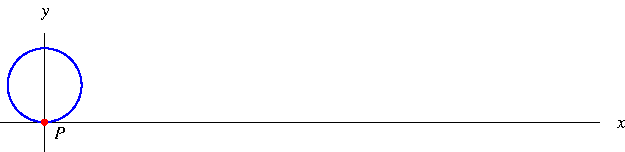
\includegraphics[width=12cm]{parametric-curves/pictures/11-01-cycloida.pdf}%
%}%
%\only<handout:0| 2>{%
%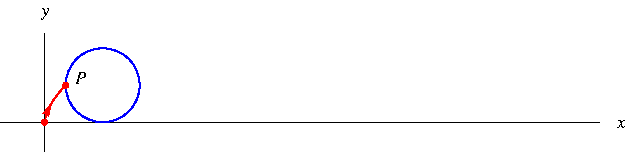
\includegraphics[width=12cm]{parametric-curves/pictures/11-01-cycloidb.pdf}%
%}%
%\only<handout:0| 3>{%
%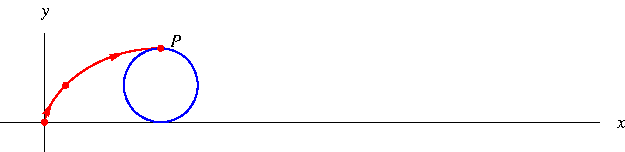
\includegraphics[width=12cm]{parametric-curves/pictures/11-01-cycloidc.pdf}%
%}%
%\only<handout:0| 4>{%
%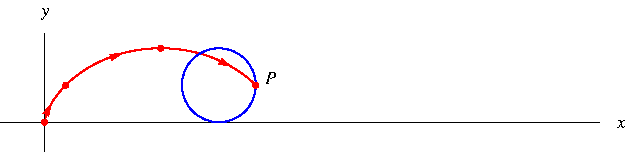
\includegraphics[width=12cm]{parametric-curves/pictures/11-01-cycloidd.pdf}%
%}%
%\only<handout:0| 5>{%
%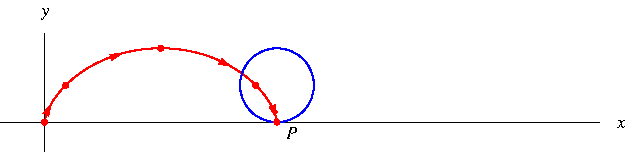
\includegraphics[width=12cm]{parametric-curves/pictures/11-01-cycloide.pdf}%
%}%
%\only<handout:0| 6>{%
%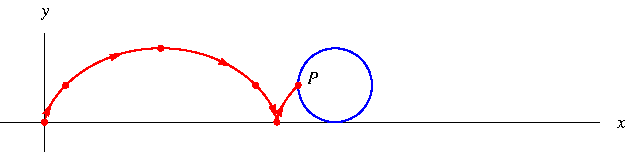
\includegraphics[width=12cm]{parametric-curves/pictures/11-01-cycloidf.pdf}%
%}%
%\only<handout:0| 7>{%
%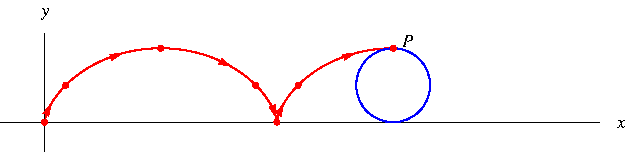
\includegraphics[width=12cm]{parametric-curves/pictures/11-01-cycloidg.pdf}%
%}%
%\only<8>{%
%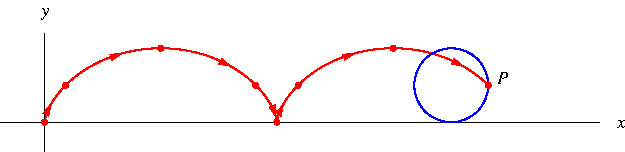
\includegraphics[width=12cm]{parametric-curves/pictures/11-01-cycloidh.pdf}%
%}%
%\only<handout:0| 9>{%
%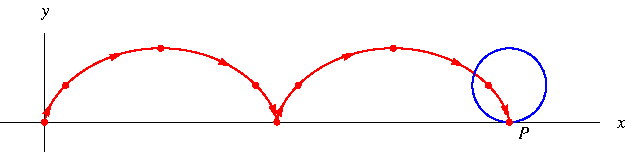
\includegraphics[width=12cm]{parametric-curves/pictures/11-01-cycloidi.pdf}%
%}%
%\only<handout:0| 10->{%
%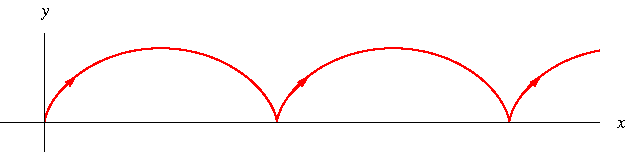
\includegraphics[width=12cm]{parametric-curves/pictures/11-01-cycloidj.pdf}%
%}%

\end{frame}
% end module cycloid-def

%%begin module polar-two-points-coincide-iff
\begin{frame}
\begin{itemize}
\item Let $P_1$ be point  with polar coordinates $(r_1, \theta_1)$.
\item Let $P_2$ be point  with polar coordinates $(r_2, \theta_2)$.
\end{itemize}

\uncover<2->{
\begin{observation}
$P_1$ coincides with $P_2$ if one of the three mutually exclusive possibilities holds:
\begin{itemize}
\item<alert@3> $r_1=r_2\neq 0$ and $\theta_2=\theta_1+2k\pi, k\in \mathbb Z $,
\item<alert@4> $r_1=-r_2\neq 0$ and $\theta_2=\theta_1+(2k+1)\pi, k\in \mathbb Z$,
\item $r_1=r_2=0 $ and $\theta$ is arbitrary.
\end{itemize}
\end{observation}
}
\begin{columns}
\column{.5\textwidth}
\only<3>{
\psset{xunit=2cm, yunit=2cm}
\begin{pspicture}(-0.9, -1.1)(2,0.75) 
\tiny 
%force a boudning box:
%\psline[linecolor=red!1](-0.1, -0.1)(-0.21,0.2)
%\psline[linecolor=red!1](1.1, 0.6)(1.1,0.61)
\psFullDotBlue{0}{0}

%Calculator input: plotCurve{}(1/10 \cos{}t, 1/10 \sin{}t, 0, -3/4 \pi)
\parametricplot[arrows=->, linecolor=\psColorGraph, plotpoints=100]{0} {3.926990817} {t 57.29578 mul cos 0.3000000 mul t 57.29578 mul sin 0.3000000 mul }
\rput[t] (0,-0.1){$O$}
\rput[l](0.3, 0.3){$\theta_1$}

\psline{->}(0,0)(2,0)
\psline[linecolor=blue](0,0)(-0.707106781, -0.707106781)
\psFullDotBlue{-0.707106781}{-0.707106781}
\rput[tl](-0.6, -0.7){$(r_1,\theta_1)$}
\end{pspicture} 
}
\uncover<4>{
\psset{xunit=2cm, yunit=2cm}
\begin{pspicture}(-0.9, -1.1)(2,0.75) 
\tiny 
%force a boudning box:
%\psline[linecolor=red!1](-0.1, -0.1)(-0.21,0.2)
\psline[linecolor=red!1](1.1, 0.5)(1.1,0.51)
\psFullDotBlue{0}{0}

%Calculator input: plotCurve{}(1/10 \cos{}t, 1/10 \sin{}t, 0, -3/4 \pi)
\parametricplot[arrows=->, linecolor=\psColorGraph, plotpoints=100]{0} {-2.35619} {t 57.29578 mul cos 0.3000000 mul t 57.29578 mul sin 0.3000000 mul }
\rput[t] (0,-0.1){$O$}
\rput[l](0.3, -0.2){$\theta_1$}

\psline{->}(0,0)(2,0)
\psline[linecolor=blue](0,0)(-0.707106781, -0.707106781)
\psFullDotBlue{-0.707106781}{-0.707106781}
\rput[tl](-0.6, -0.7){$(r_1,\theta_1)$}
\end{pspicture} 
}

%\ \uncover<1->{%
%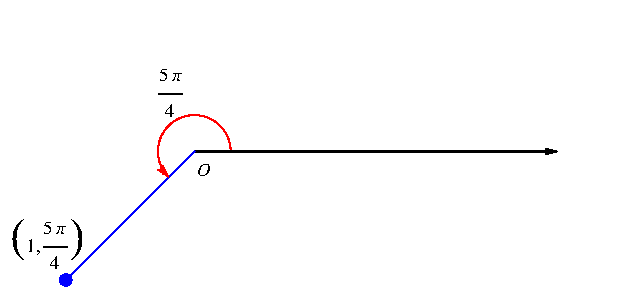
\includegraphics[height=3cm]{polar-curves/pictures/11-03-ex1a.pdf}%
%}%

%\ \uncover<2->{%
%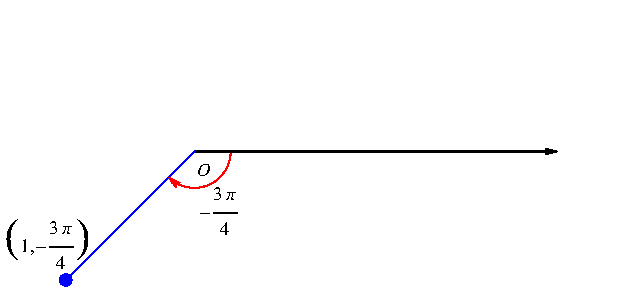
\includegraphics[height=3cm]{polar-curves/pictures/11-03-ex1b.pdf}%
%}%

\vspace{2cm}
\column{.5\textwidth}
\only<3>{
\psset{xunit=2cm, yunit=2cm}
\begin{pspicture}(-0.9, -1.1)(2,0.75) 
\tiny 
%force a boudning box:
%\psline[linecolor=red!1](-0.1, -0.1)(-0.21,0.2)
%\psline[linecolor=red!1](1.1, 0.6)(1.1,0.61)
\psFullDotBlue{0}{0}

%Calculator input: plotCurve{}(1/50 t \cos{}t+3/20 \cos{}t, 1/50 t \sin{}t+3/20 \sin{}t, 0, 13/4 \pi)
\parametricplot[arrows=->, linecolor=\psColorGraph, plotpoints=400] {0} {10.2102} {t 57.29578 mul cos 0.1500000 mul t 57.29578 mul cos t mul 0.0200000 mul add t 57.29578 mul sin 0.1500000 mul t 57.29578 mul sin t mul 0.0200000 mul add }

\rput[t] (0,-0.1){$O$}
\rput[l](0.3, 0.3){$\theta_2=\theta_1+2\pi$}

\psline{->}(0,0)(2,0)
\psline[linecolor=blue](0,0)(-0.707106781, -0.707106781)
\psFullDotBlue{-0.707106781}{-0.707106781}
\rput[tl](-0.6, -0.7){$(r_2, \theta_2)=(r_1,\theta_1+2\pi)$}
\end{pspicture} 
}

\uncover<4>{
\psset{xunit=2cm, yunit=2cm}
\begin{pspicture}(-0.9, -1.1)(2,0.75) 
\tiny 
%force a boudning box:
%\psline[linecolor=red!1](-0.1, -0.1)(-0.21,0.2)
\psline[linecolor=red!1](1.1, 0.5)(1.1,0.51)
\psFullDotBlue{0}{0}

%Calculator input: plotCurve{}(1/10 \cos{}t, 1/10 \sin{}t, 0, -3/4 \pi)
\parametricplot[arrows=->, linecolor=\psColorGraph, plotpoints=100]{0} {0.785398163} {t 57.29578 mul cos 0.3000000 mul t 57.29578 mul sin 0.3000000 mul }
\rput[t] (0,-0.1){$O$}
\rput[l](0.35, 0.15){$\theta_2=\theta_1+\pi$}

\psline{->}(0,0)(2,0)
\psline[linecolor=blue](0,0)(-0.707106781, -0.707106781)
\psFullDotBlue{-0.707106781}{-0.707106781}
\psline[linestyle=dashed](0,0)(0.707106781, 0.707106781)
\psFullDotBlack{0.707106781}{0.707106781}
\rput[tl](-0.6, -0.7){$(r_2, \theta_2)=(-r_1,\theta_1+\pi)$}
\end{pspicture} 
}
%\ \uncover<3->{%
%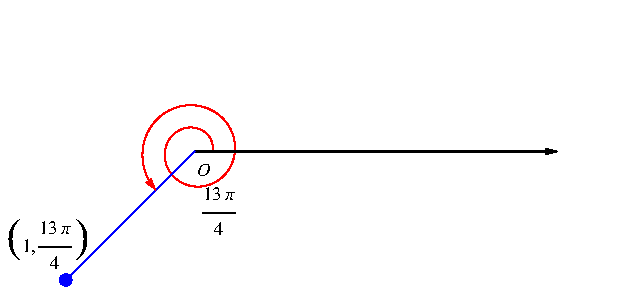
\includegraphics[height=3cm]{polar-curves/pictures/11-03-ex1c.pdf}%
%}%

%\ \uncover<4->{%
%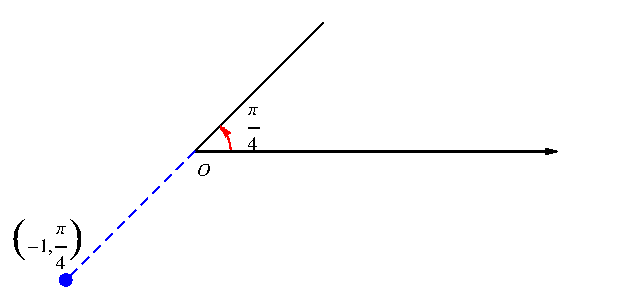
\includegraphics[height=3cm]{polar-curves/pictures/11-03-ex1d.pdf}%
%}%

\vspace{2cm}
\end{columns}
\end{frame}
%end module polar-two-points-coincide-iff

%% begin module polar-intersection-ex3
\begin{frame}
\begin{example} %[Example 3, p. 688]
Find all points of intersection of the polar curves $r = \frac{1}{2}$ and $r = \cos (2\theta)$.
\begin{columns}[c]
\column{.4\textwidth}

\psset{xunit=1.8cm, yunit=1.8cm}
\begin{pspicture}(-1.5, -1.5)(1.5,1.5)
\tiny
\fcAxesStandard{-1.4}{-1.4}{1.4}{1.4}
%Calculator command: drawPolar{}(1/2, 0, 2 \pi)
\parametricplot[linecolor=\fcColorGraph, plotpoints=1000, algebraic=false]{0}{6.28319}{ 0.5 t 57.29578 mul cos mul 0.5 t 57.29578 mul sin mul }
%Calculator command: drawPolar{}(\cos{}(2 t), 0, 2 \pi)
\parametricplot[linecolor=\fcColorGraph, plotpoints=1000, algebraic=false]{0}{6.28319}{t 2 mul 57.29578 mul cos t 57.29578 mul cos mul t 2 mul 57.29578 mul cos t 57.29578 mul sin mul }

\rput[tr](-0.8, -0.8){$r=\frac{1}{2}$}
\psline{->}(-0.75, -0.75)(-0.353553391, -0.353553391)
\rput[lt] (0.2, -1){$r=\cos (2\theta)$}

\uncover<4->{
\fcFullDotBlack{0.433013}{0.25}
\fcFullDotBlack{-0.433013}{0.25}
\fcFullDotBlack{-0.433013}{-0.25}
\fcFullDotBlack{0.433013}{-0.25}
}
\uncover<6->{
\fcFullDotBlack{0.25}{0.433013}
\fcFullDotBlack{0.25}{-0.433013}
\fcFullDotBlack{-0.25}{-0.433013}
\fcFullDotBlack{-0.25}{0.433013}
}
\uncover<9>{
\pscircle*[linecolor=red](0.433013,0.25){0.09}
\pscircle*[linecolor=red](-0.433013,0.25){0.09}
\pscircle*[linecolor=red](-0.433013,-0.25){0.09}
\pscircle*[linecolor=red](0.433013,-0.25){0.09}
}
\uncover<10>{
\pscircle*[linecolor=red](0.25,0.433013){0.09}
\pscircle*[linecolor=red](0.25,-0.433013){0.09}
\pscircle*[linecolor=red](-0.25,-0.433013){0.09}
\pscircle*[linecolor=red](-0.25,0.433013){0.09}
}
\end{pspicture}

%\ \only<handout:0| -3>{%
%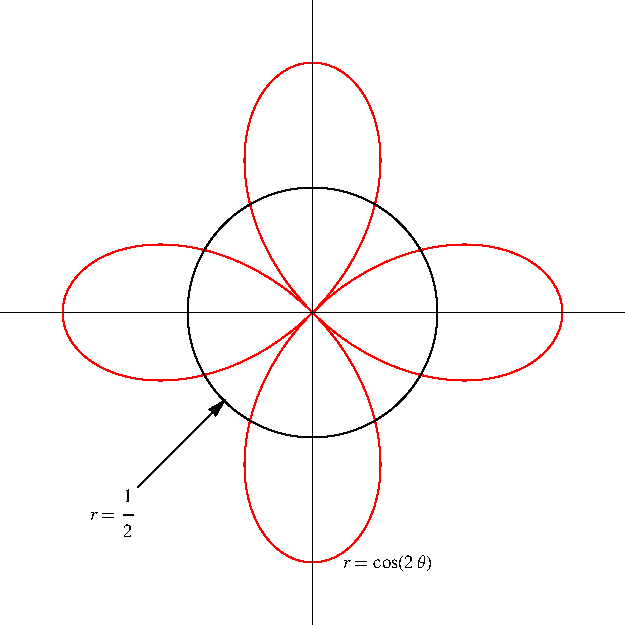
\includegraphics[height=5cm]{polar-curves/pictures/11-04-ex3a.pdf}%
%}%
%\only<handout:0| 4-5>{%
%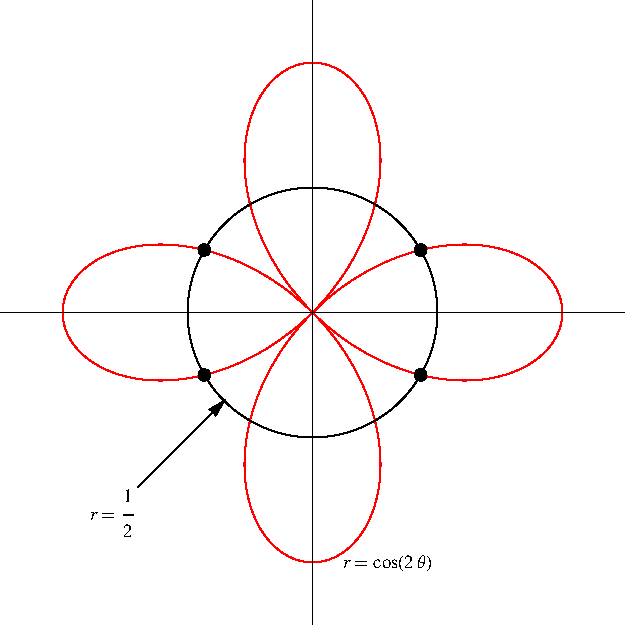
\includegraphics[height=5cm]{polar-curves/pictures/11-04-ex3b.pdf}%
%}%
%\only<6-8>{%
%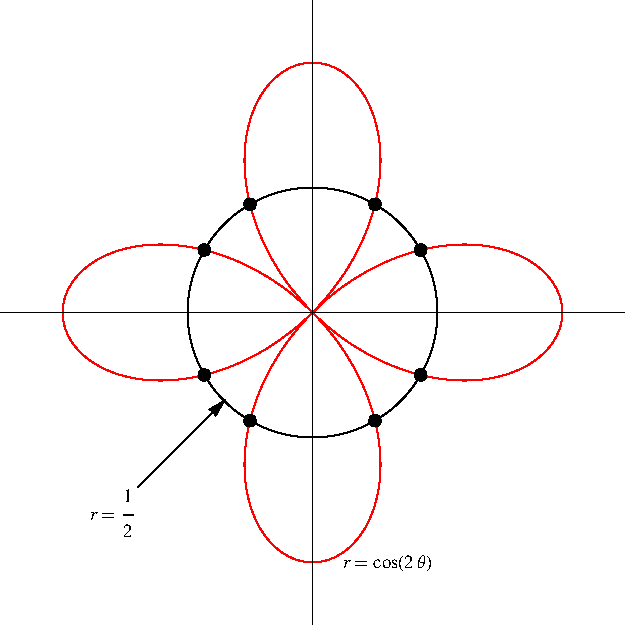
\includegraphics[height=5cm]{polar-curves/pictures/11-04-ex3c.pdf}%
%}%
%\only<handout:0| 9>{%
%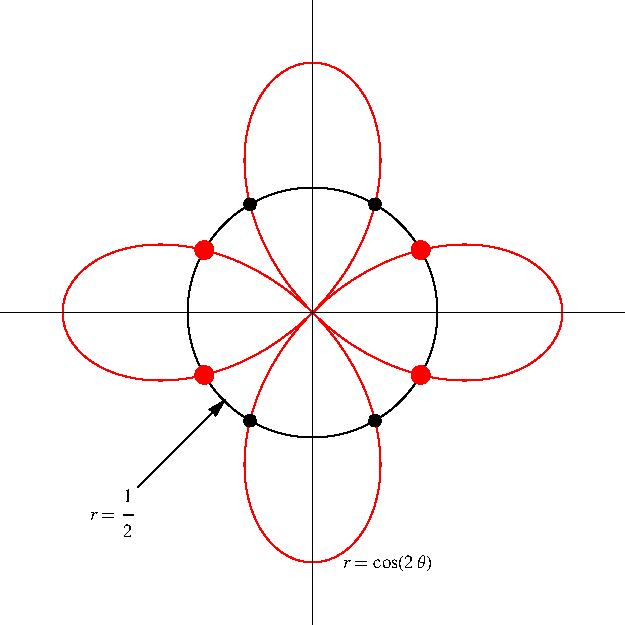
\includegraphics[height=5cm]{polar-curves/pictures/11-04-ex3d.pdf}%
%}%
%\only<handout:0| 10->{%
%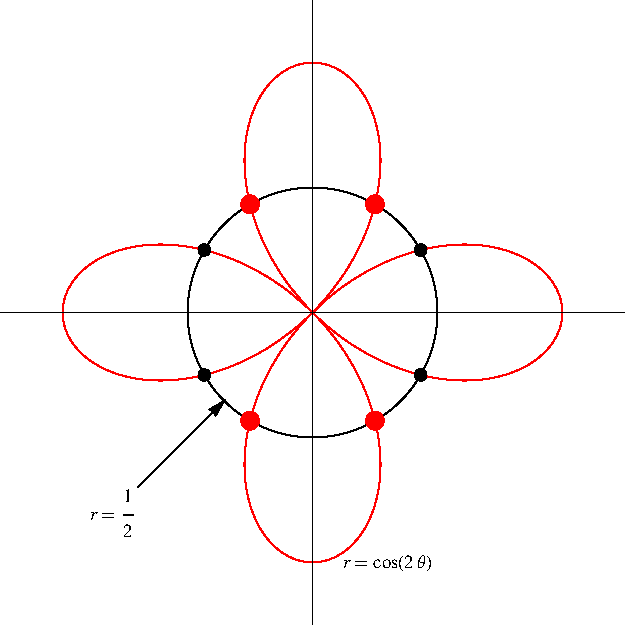
\includegraphics[height=5cm]{polar-curves/pictures/11-04-ex3e.pdf}%
%}%
\column{.6\textwidth}
\abovedisplayskip=0pt
\belowdisplayskip=0pt
\begin{eqnarray*}
\uncover<2->{%
\cos 2\theta%
}%
& \uncover<2->{ = } &%
\uncover<2->{%
\frac{1}{2}%
}\\%
\uncover<3->{%
2\theta%
}%
& \uncover<3->{ = } &%
\uncover<3->{%
\frac{\pi}{3}, \frac{5\pi}{3}, \frac{7\pi}{3}, \frac{11\pi}{3}%
}\\%
\uncover<4->{%
\theta%
}%
& \uncover<4->{ = } &%
\uncover<4->{%
\frac{\pi}{6}, \frac{5\pi}{6}, \frac{7\pi}{6}, \frac{11\pi}{6}%
}%
\end{eqnarray*}
\begin{itemize}
\item<5->  This only gives four points.
\item<6->  There are actually eight.
\item<7->  The circle $r = \frac{1}{2}$ also has polar equation $r = -\frac{1}{2}$.
\item<8->  To find all eight points, solve \alertNoH{ 9}{$\cos (2\theta )= \frac{1}{2}$} and \alertNoH{ 10}{$\cos (2\theta) = -\frac{1}{2}$}.
\end{itemize}
\end{columns}
\end{example}
\end{frame}
% end module polar-intersection-ex3


%% begin module trig-substitutions-ex3
\begin{frame}
\begin{example} %[Example 3, p. 505]
\begin{columns}[c]
\column{.4\textwidth}
Find $\int \frac{1}{x^2 \sqrt{x^2+4}}\diff x$.
\begin{itemize}
\item<2->  Let \alert<handout:0| 3-4,7,14,20>{$x = \uncover<4->{2\tan \theta}$}\uncover<4->{, where \alert<handout:0| 10>{$-\pi /2 \leq \theta \leq \pi / 2$}.}
\item<2->  Then \alert<handout:0| 5-6,13>{$\diff x = \uncover<6->{2\sec^2 \theta\diff \theta}$}\uncover<6->{.}
\end{itemize}
\column{.6\textwidth}
\begin{center}
\psset{xunit=2cm, yunit=2cm}
\begin{pspicture}(-0.15,-0.3)(2.3,1.2)
\psframe*[linecolor=white](-0.1,-0.3)(2.3,1.2)
\psline(0,0)(2, 0)(2,1)(0,0)
\psline(1.9,0)(1.9, 0.1)(2,0.1)
\fcAngle{0}{0.463648}{0.4}{$\theta$}
\uncover<handout:0|20->{
\rput[l](2.1, 0.5){$x$}
\rput[t](1, -0.1){$2$}
}
\uncover<handout:0|21->{
\rput[br](1, 0.55){$\sqrt{x^2+4}$}
}
%bounding box for pdflatex compilation:
\psline[linecolor=red!1](-0.11, -0.3 )(-0.105, -0.3)
\psline[linecolor=red!1](2.3, 1.21)(2.3, 1.205)
\end{pspicture}
%\ \only<handout:0| -19>{%
%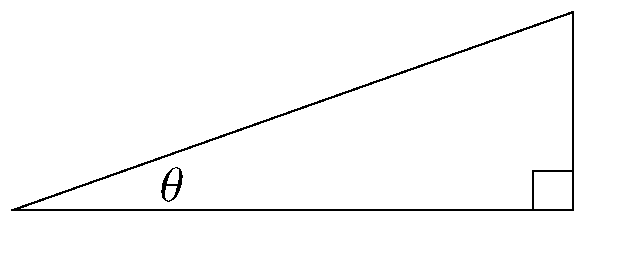
\includegraphics[height=3cm]{trig-substitution/pictures/08-03-ex3a.pdf}%
%}%
%\only<handout:0| 20>{%
%\includegraphics[height=3cm]{trig-substitution/pictures/08-03-ex3b.pdf}%
%}%
%\only<21->{%
%\includegraphics[height=3cm]{trig-substitution/pictures/08-03-ex3c.pdf}%
%}%
\end{center}
\end{columns}
\abovedisplayskip=0pt
\belowdisplayskip=0pt
\[
\uncover<2->{%
\alert<handout:0| 12>{%
\sqrt{\alert<handout:0| 7>{x^2} + 4} =
}%
}%
\uncover<7->{%
\sqrt{\alert<handout:0| 7>{4\tan^2 \theta} + 4} =
}%
\uncover<8->{%
\sqrt{4 \sec^2 \theta} =
}%
\uncover<9->{%
2 |\sec  \theta | =
}%
\uncover<10->{%
\alert<handout:0| 12>{%
2 \sec  \theta
}%
}%
\]
\abovedisplayskip=0pt
\belowdisplayskip=0pt
\begin{eqnarray*}
\uncover<11->{%
\int \frac{\alert<handout:0| 13>{\diff x}}{\alert<handout:0| 14>{x^2}\alert<handout:0| 12>{\sqrt{x^2+4}}}%
}%
& \uncover<11->{ = } & %
\uncover<11->{%
\int\frac{\alert<handout:0| 13>{2\sec^2 \theta \diff \theta}}{\alert<handout:0| 14>{4\tan^2 \theta}\cdot \alert<handout:0| 12>{2\sec \theta}}
}%
\uncover<15->{%
 = \frac{1}{4}\int \frac{\cos \theta}{\sin^2\theta} \diff \theta
}\\%
\uncover<16->{%
\textrm{Let } \alert<handout:0| 19>{u = \sin \theta} :%
}%
& \uncover<17->{ = } & %
\uncover<17->{%
\frac{1}{4} \int \frac{\diff u}{u^2}
}  \uncover<18->{ = }  \uncover<18->{%
\frac{1}{4} \left( -\alert<handout:0| 19>{\frac{1}{u}}\right)  + C
}\\%
& \uncover<19->{ = } & %
\uncover<19->{%
 -\frac{\alert<handout:0| 19,22-23>{\csc \theta}}{4} + C
}%
\uncover<23->{%
=  -\frac{\alert<handout:0| 23>{\sqrt{x^2+4}}}{4\alert<handout:0| 23>{x}} + C
}%
\end{eqnarray*}
\end{example}
\end{frame}
% end module trig-substitutions-ex3

%% begin module trig-substitutions-ex1
\begin{frame}
\begin{example} %[Example 1, p. 504]
\begin{columns}[c]
\column{.4\textwidth}
Evaluate $\int \frac{\sqrt{9-x^2}}{x^2}\diff x$.
\begin{itemize}
\item<2->  Let \alert<handout:0| 3-4,7,14,18>{$x = \uncover<4->{3\sin \theta}$}\uncover<4->{, where \alert<handout:0| 10>{$-\pi /2 \leq \theta \leq \pi / 2$}.}
\item<2->  Then \alert<handout:0| 5-6,13>{$\diff x = \uncover<6->{3\cos \theta\diff \theta}$}\uncover<6->{.}
\end{itemize}
\column{.6\textwidth}
\begin{center}
\psset{xunit=1.5cm, yunit=1.5cm}
\begin{pspicture}(-0.15,-0.4)(3.3,1.2)
\psframe*[linecolor=white](-0.1,-0.4)(3.3,1.2)
\psline(0,0)(3, 0)(3,1)(0,0)
\psline(2.9,0)(2.9, 0.1)(3,0.1)
\fcAngle{0}{0.339837}{0.6}{$\theta$}
\uncover<handout:0|18->{
\rput[l](3.1, 0.5){$x$}
\rput[br](1.5, 0.55){$3$}
}
\uncover<handout:0|19->{
\rput[t](1.5, -0.1){$\sqrt{9-x^2} $}
}
%bounding box for pdflatex compilation:
\psline[linecolor=red!1](-0.11, -0.4 )(-0.105, -0.4)
\psline[linecolor=red!1](3.3, 1.21)(3.3, 1.205)
\end{pspicture}
%\ \only<handout:0| -17>{%
%\includegraphics[height=3cm]{trig-substitution/pictures/08-03-ex1a.pdf}%
%}%
%\only<handout:0| 18>{%
%\includegraphics[height=3cm]{trig-substitution/pictures/08-03-ex1b.pdf}%
%}%
%\only<19->{%
%\includegraphics[height=3cm]{trig-substitution/pictures/08-03-ex1c.pdf}%
%}%
\end{center}
\end{columns}
\abovedisplayskip=0pt
\belowdisplayskip=0pt
\[
\uncover<2->{%
\alert<handout:0| 12>{%
\sqrt{9 - \alert<handout:0| 7>{x^2}} =
}%
}%
\uncover<7->{%
\sqrt{9 - \alert<handout:0| 7>{9\sin^2 \theta}} =
}%
\uncover<8->{%
\sqrt{9 \cos^2 \theta} =
}%
\uncover<9->{%
3 |\cos  \theta | =
}%
\uncover<10->{%
\alert<handout:0| 12>{%
3 \cos  \theta
}%
}%
\]
\abovedisplayskip=0pt
\belowdisplayskip=0pt
\begin{eqnarray*}
\uncover<11->{%
\int \frac{\alert<handout:0| 12>{\sqrt{9-x^2}}}{\alert<handout:0| 14>{x^2}}\alert<handout:0| 13>{\diff x}%
}%
& \uncover<11->{ = } & %
\uncover<11->{%
\int\frac{\alert<handout:0| 12>{3\cos \theta}}{\alert<handout:0| 14>{9\sin^2 \theta}}\alert<handout:0| 13>{3\cos \theta \diff \theta}
}%
\uncover<15->{%
 = \int \cot^2 \theta \diff \theta
}\\%
& \uncover<16->{ = } & %
\uncover<16->{%
 \int (\csc^2 \theta  - 1)\diff \theta
}  \uncover<17->{ = }  \uncover<17->{%
 -\alert<handout:0| 20-21>{\cot \theta} - \theta + C
}\\%
& \uncover<21->{ = } & %
\uncover<21->{%
 -\alert<handout:0| 21>{\frac{\sqrt{9-x^2}}{x}} - \Arcsin \left( \frac{x}{3}\right) + C
}%
\end{eqnarray*}
\end{example}
\end{frame}
% end module trig-substitutions-ex1

%% begin module trig-substitutions-ex5
\begin{frame}
\begin{example} %[Example 5, p. 506]
\begin{columns}[c]
\column{.4\textwidth}
Find $\int \frac{\diff x}{\sqrt{x^2-a^2}}$, \alert<handout:0| 9>{$a > 0$}.
\begin{itemize}
\item<2->  \alert<handout:0| 3-4,7,16,20>{$x = \uncover<4->{a\sec \theta}$}\uncover<4->{,  \alert<handout:0| 10>{$0 < \theta < \pi / 2$ or $\pi < \theta < 3\pi /2$}.}
\item<2->  \alert<handout:0| 5-6,13>{$\diff x = \uncover<6->{a\sec \theta\tan \theta \diff \theta}$}\uncover<6->{.}
\end{itemize}
\column{.6\textwidth}
\begin{center}
\ \only<handout:0| -15>{%
\includegraphics[height=2.8cm]{trig-substitution/pictures/08-03-ex5a.pdf}%
}%
\only<handout:0| 16>{%
\includegraphics[height=2.8cm]{trig-substitution/pictures/08-03-ex5b.pdf}%
}%
\only<17->{%
\includegraphics[height=2.8cm]{trig-substitution/pictures/08-03-ex5c.pdf}%
}%
\end{center}
\end{columns}
\abovedisplayskip=0pt
\belowdisplayskip=0pt
\[
\uncover<2->{%
\alert<handout:0| 12>{%
\sqrt{\alert<handout:0| 7>{x^2}-a^2} = 
}%
}%
\uncover<7->{%
\sqrt{\alert<handout:0| 7>{a^2\sec^2 \theta}-a^2} = 
}%
\uncover<8->{%
\sqrt{a^2 \tan^2 \theta} = 
}%
\uncover<9->{%
a |\tan  \theta | = 
}%
\uncover<10->{%
\alert<handout:0| 12>{%
a \tan  \theta  
}%
}%
\]
\abovedisplayskip=0pt
\belowdisplayskip=0pt
\begin{eqnarray*}
\uncover<11->{%
\int \frac{\alert<handout:0| 13>{\diff x}}{\alert<handout:0| 12>{\sqrt{x^2-a^2}}}%
}%
& \uncover<11->{ = } & %
\uncover<11->{%
\int\frac{\alert<handout:0| 13>{a\sec \theta \tan \theta \diff \theta}}{\alert<handout:0| 12>{a\tan \theta}}%
}%
\uncover<14->{%
 = \int \sec \theta \diff \theta
}\\%
& \uncover<15->{ = } & %
\uncover<15->{%
\ln | \alert<handout:0| 20>{\sec \theta} + \alert<handout:0| 18-19>{\tan \theta} | + C%
}  \uncover<19->{ = }  \uncover<19->{%
\ln \left| \alert<handout:0| 20>{\frac{x}{\alert<handout:0| 21>{a}}} + \alert<handout:0| 19>{\frac{\sqrt{x^2-a^2}}{\alert<handout:0| 21>{a}}}\right| + C
}\\%
& \uncover<21->{ = } & %
\uncover<21->{%
\ln \left| x + \sqrt{x^2 - a^2}\right| \only<handout:0| -22>{\alert<handout:0| 21-22>{- \ln a} \alert<handout:0| 22>{+ C}}\only<23->{\alert<handout:0| 23>{ + C_1}}%
}%
\end{eqnarray*}
\end{example}
\end{frame}
% end module trig-substitutions-ex5

%% begin module parametric-tangents-ex1
\begin{frame}[t]
\begin{example}
\begin{columns}
\column{0.25\textwidth}
\psset{xunit=0.4cm, yunit=0.4cm}
\begin{pspicture}(-0.9, -2.4)(4.4,2.499997)
\tiny
\fcAxesStandard{-0.650000}{-2.150000}{4.150000}{2.149997}
%Calculator input: plotCurve{}(t^{2}, t^{3}-3 t, -2, 2)
\parametricplot[linecolor=\fcColorGraph, plotpoints=1000]{-2}{2}{t 2.0000000 exp t -3.0000000 mul t 3.0000000 exp add }
\end{pspicture}
\column{0.75\textwidth}
A curve $C$ is defined by $x = t^2, y = t^3 - 3t$.
\end{columns}
\begin{enumerate}
\item Show $C$ traverses $(x,y)=(3,0)$ for two values of $t$; find the tangent slopes for both of these values.
\item Find the points on $C$ where the tangents are horizontal or vertical.
\item Find two intervals where we can write $y$ as a function of $x$.
\item Determine concavity intervals of the functions found in item 3.
\end{enumerate}
\end{example}
\vspace{4cm}
\end{frame}




\begin{frame}[t]
\begin{example}
\begin{columns}
\column{0.25\textwidth}
\psset{xunit=0.4cm, yunit=0.4cm}
\begin{pspicture}(-0.9, -2.4)(4.4,2.499997)
\tiny%
\fcAxesStandard{-0.650000}{-2.150000}{4.150000}{2.149997}%
%Calculator input: plotCurve{}(t^{2}, t^{3}-3 t, -2, 2)
\parametricplot[linecolor=\fcColorGraph, plotpoints=1000]{-2}{2}{t 2.0000000 exp t -3.0000000 mul t 3.0000000 exp add }%
\fcFullDotBlue{3}{0}%
\uncover<15->{%
\psline[linecolor=\fcColorTangent](2,1.732050808)(4,-1.732050808)%
\psline[linecolor=\fcColorTangent](2,-1.732050808)(4,1.732050808)%
}%
\end{pspicture}
\column{0.75\textwidth}
A curve $C$ is defined by \alert<handout:0| 2>{$x = t^2, y = t^3 - 3t$}.
\end{columns}
\begin{enumerate}
\item Show $C$ traverses $(x,y)=(3,0)$ for two values of $t$; find the tangent slopes for both of these values.
\end{enumerate}
\begin{itemize}
\item<2-| alert@3-4>  $3 = \alert<handout:0| 2>{x = t^2}$ \ if \ $t = $ \uncover<4->{$\pm \sqrt{3}$.}
\item<2-| alert@5-6>  $0 = \alert<handout:0| 2>{y = t^3 - 3t} = t(t^2-3)$\  if \ $t = $ \uncover<6->{$0$\  or\  $\pm \sqrt{3}$.}
\item<7->  Therefore the point $(3,0)$ is traversed when $t$ equals $\sqrt{3}$ or $-\sqrt{3}$.
\item<8-> $ \uncover<8->{ \frac{\diff y}{\diff x} = \frac{\alert<handout:0| 9-10>{\diff y / \diff t}}{\alert<handout:0| 11-12>{\diff x / \diff t}} %
} \uncover<9->{= \frac{\alert<handout:0| 10>{\uncover<10->{3t^2-3 }}}{\alert<handout:0| 12>{\uncover<12->{2t }}}}$\uncover<12->{\quad .}
\item<13->
Plug in $t = \pm \sqrt{3}$:
$\displaystyle
\uncover<13->{%
\frac{\diff y}{\diff x} _{|t = \pm \sqrt{3}} = \frac{3(\pm \sqrt{3})^2 - 3}{2(\pm \sqrt{3})} = %
}%
\uncover<14->{%
\pm \frac{6}{2\sqrt{3}} = \pm \sqrt{3}%
}%
$
\uncover<15->{%
Therefore the tangents at $(3,0)$ have slopes $\pm \sqrt{3}$.
}%
\end{itemize}
\end{example}
\vspace{4cm}
\end{frame}

\begin{frame}[t]
\begin{example}
\begin{columns}
\column{0.25\textwidth}
\psset{xunit=0.4cm, yunit=0.4cm}
\begin{pspicture}(-0.9, -2.4)(4.4,2.499997)
\tiny
\fcAxesStandard{-0.650000}{-2.150000}{4.150000}{2.149997}
%Calculator input: plotCurve{}(t^{2}, t^{3}-3 t, -2, 2)
\parametricplot[linecolor=\fcColorGraph, plotpoints=1000]{-2}{2}{t 2.0000000 exp t -3.0000000 mul t 3.0000000 exp add }
\uncover<6->{%
\fcFullDotBlue{1}{2}
\fcFullDotBlue{1}{-2}
\psline[linecolor=\fcColorTangent](0.1,2)(1.9,2)
\psline[linecolor=\fcColorTangent](0.1,-2)(1.9,-2)
}%
\uncover<10->{%
\fcFullDotBlue{0}{0}
\psline[linecolor=\fcColorTangent](0,-1)(0,1)
}%
\end{pspicture}
\column{0.75\textwidth}
A curve $C$ is defined by $x = t^2, y = t^3 - 3t$.
\end{columns}
\begin{enumerate}
\setcounter{enumi}{1}
%\item  Show that $C$ has two tangents at $(3,0)$ and find their slopes.
\item  Find the points on $C$ where the tangents are horizontal or vertical.
%\item  Determine where the curve is concave up or down.
\end{enumerate}
\begin{columns}[t]
\column{.5\textwidth}
Horizontal tangent:
\abovedisplayskip=0pt
\belowdisplayskip=0pt
\begin{eqnarray*}
\frac{\diff y}{\diff t} & = & 0\\
\uncover<2->{%
3t^2 - 3%
}%
& \uncover<2->{ = } & %
\uncover<2->{%
0
}\\%
\uncover<3->{%
3(t^2 - 1)%
}%
& \uncover<3->{ = } & %
\uncover<3->{%
0
}\\%
\uncover<4->{%
t%
}%
& \uncover<4->{ = } & %
\uncover<4->{%
\pm 1%
}%
\end{eqnarray*}
\uncover<5->{$\frac{\diff x}{\diff t} \neq 0$ when $t = \pm 1$, so there are horizontal tangents when $t = \pm 1$.}

\uncover<6->{%
The points are $(1, 2)$ and $(1, -2)$.
}%
\column{.5\textwidth}
Vertical tangent:
\abovedisplayskip=0pt
\belowdisplayskip=0pt
\begin{eqnarray*}
\frac{\diff x}{\diff t} & = & 0\\
\uncover<7->{%
2t%
}%
& \uncover<7->{ = } & %
\uncover<7->{%
0%
}\\%
\uncover<8->{%
t%
}%
& \uncover<8->{ = } & %
\uncover<8->{%
0%
}%
\end{eqnarray*}
\uncover<9->{$\frac{\diff y}{\diff t} \neq 0$ when $t =  0$, so there is a vertical tangent when $t = 0$.}

\uncover<10->{%
The points is $(0,0)$.
}%
\end{columns}
\end{example}
\vspace{4cm}
\end{frame}



\begin{frame}[t]
\begin{example} %[Example 1, p. 667]
\begin{columns}
\column{0.25\textwidth}
\psset{xunit=0.4cm, yunit=0.4cm}
\begin{pspicture}(-0.9, -2.4)(4.4,2.499997)
\tiny
\fcAxesStandard{-0.650000}{-2.150000}{4.150000}{2.149997}
\uncover<1-4,6->{%
%Calculator input: plotCurve{}(t^{2}, t^{3}-3 t, -2, 2)
\parametricplot[linecolor=\fcColorGraph, plotpoints=1000]{-2}{0}{t 2.0000000 exp t -3.0000000 mul t 3.0000000 exp add }%
}%
\uncover<1-5>{%
\parametricplot[linecolor=\fcColorGraph, plotpoints=1000]{0}{2}{t 2.0000000 exp t -3.0000000 mul t 3.0000000 exp add }%
}%
\end{pspicture}
\column{0.75\textwidth}
A curve $C$ is defined by $x = t^2, y = t^3 - 3t$.
\end{columns}
\begin{enumerate}
\setcounter{enumi}{2}
%\item  Show that $C$ has two tangents at $(3,0)$ and find their slopes.
%\item  Find the points on $C$ where the tangents are horizontal or vertical.
\item  Find two intervals where we can write $y$ as a function of $x$.
\end{enumerate}
\uncover<2->{From $x=t^2$ we have that $t=\pm \sqrt{x}$.} \uncover<3->{Therefore, when $t>0$, we have that $t=\sqrt{x}$.} \uncover<4->{Since that determines uniquely $t$ via $x$, this means that for $t>0$  $y$ is a function of $x$.} \uncover<5->{In other words, for $t>0$, the curve satisfies the vertical line test. } \uncover<6->{Similarly we conclude that when $t<0$, $y$ is a function of $x$.}
\end{example}
\vspace{5cm}
\end{frame}

\begin{frame}[t]
\begin{example} %[Example 1, p. 667]
\begin{columns}
\column{0.25\textwidth}
\psset{xunit=0.4cm, yunit=0.4cm}
\begin{pspicture}(-0.9, -2.4)(4.4,2.499997)
\tiny
\fcAxesStandard{-0.650000}{-2.150000}{4.150000}{2.149997}
\uncover<1-11,13->{%
%Calculator input: plotCurve{}(t^{2}, t^{3}-3 t, -2, 2)
\parametricplot[linecolor=\fcColorGraph, plotpoints=1000]{-2}{0}{t 2.0000000 exp t -3.0000000 mul t 3.0000000 exp add }%
}%
\uncover<1-12>{%
\parametricplot[linecolor=\fcColorGraph, plotpoints=1000]{0}{2}{t 2.0000000 exp t -3.0000000 mul t 3.0000000 exp add }%
}%
\end{pspicture}
\column{0.75\textwidth}
A curve $C$ is defined by $x = t^2, y = t^3 - 3t$.
\end{columns}
\begin{enumerate}
\setcounter{enumi}{3}
\item  Determine the concavity intervals of the functions found in item 3.
\end{enumerate}
\uncover<2->{Find the second derivative:}%

$\begin{array}{rcl}
\displaystyle \uncover<2->{%
\frac{\diff^2 y}{\diff x^2}%
}%
& \uncover<2->{ = } &%
\displaystyle \uncover<2->{%
\frac{\frac{\diff}{\diff t}\left( \alert<handout:0| 3-4>{\frac{\diff y}{\diff x}}\right)}{\alert<handout:0| 5-6>{\frac{\diff x}{\diff t}}}%
}  \uncover<3->{ = }  \uncover<3->{%
\frac{\frac{\diff}{\diff t}\left( \alert<handout:0| 3-4,7>{\uncover<4->{\frac{3t^2-3}{2t}}}\right)}{\alert<handout:0| 5-6>{\uncover<6->{2t}}}%
}\\%
& \uncover<7->{ = } &\displaystyle
\uncover<7->{%
\frac{\alert<handout:0| 8-9>{\frac{\diff}{\diff t}\left( \alert<handout:0| 7>{\frac{3}{2}\left( t - \frac{1}{t}\right)}\right)}}{2t}%
}  \uncover<8->{ = }  \uncover<8->{%
\frac{\alert<handout:0| 8-9>{\uncover<9->{\frac{3}{2} + \frac{3}{2t^2} }}}{2t}%
}\\%
& \uncover<10->{ = } &\displaystyle
\uncover<10->{%
\frac{\frac{3t^2 + 3}{2t^2}}{2t}%
}  \uncover<11->{ = } \uncover<11->{%
\frac{3(t^2 + 1)}{4t^3}%
}%
\end{array}
$

\uncover<12->{%
Therefore $y$ as a function of $x$ (which is a function of $t$) is concave up when $t > 0$}\uncover<13->{ and concave down when $t < 0$.}%
\end{example}
\vspace{4cm}
\end{frame}
% end module parametric-tangents-ex1


%% begin module arc-length-intro
\begin{frame}
\frametitle{Arc Length}
\begin{center}

\psset{xunit=2cm, yunit=2cm}
\begin{pspicture}(-1, -1)(1,1)
\tiny %
\parametricplot[linecolor=\fcColorGraph, plotpoints=1000, algebraic=true]{0}{6.283185307}{cos(t)|sin(t)}%
\uncover<3>{ %
\fcRegularNgon[linecolor=\fcColorTangent]{3}{1}%
}
\uncover<4>{ %
\fcRegularNgon[linecolor=\fcColorTangent]{4}{1}%
}
\uncover<5>{ %
\fcRegularNgon[linecolor=\fcColorTangent]{6}{1}%
}
\uncover<6>{ %
\fcRegularNgon[linecolor=\fcColorTangent]{8}{1}%
}
\uncover<7>{ %
\fcRegularNgon[linecolor=\fcColorTangent]{12}{1}%
}
\uncover<8>{ %
\fcRegularNgon[linecolor=\fcColorTangent]{16}{1}%
}
\uncover<9>{ %
\fcRegularNgon[linecolor=\fcColorTangent]{32}{1}%
}
\end{pspicture}

\uncover<1-9>{}
%\ \only<-2>{%
%\includegraphics[height=4cm]{arc-length/pictures/09-01-circlea.pdf}%
%}%
%\only<handout:0| 3>{%
%\includegraphics[height=4cm]{arc-length/pictures/09-01-circleb.pdf}%
%}%
%\only<handout:0| 4>{%
%\includegraphics[height=4cm]{arc-length/pictures/09-01-circlec.pdf}%
%}%
%\only<handout:0| 5>{%
%\includegraphics[height=4cm]{arc-length/pictures/09-01-circled.pdf}%
%}%
%\only<handout:0| 6>{%
%\includegraphics[height=4cm]{arc-length/pictures/09-01-circlee.pdf}%
%}%
%\only<handout:0| 7->{%
%\includegraphics[height=4cm]{arc-length/pictures/09-01-circlef.pdf}%
%}%
\end{center}
\begin{itemize}
\item  What do we mean by the length of a curve?
\item<2->  The length of a polygon is easy to compute: add up the length of the line segments that form the polygon.
\item<3->  If the curve is a circle, approximate it by a polygon.
\item<4->  Then take the limit as the number of segments of the polygon goes to $\infty$.
\end{itemize}
\end{frame}
% end module arc-length-intro

%%begin module arc-length-derivation-parametric
{% scoping block for the following command:
%Calculator input: plotCurve{}(t, 8 t^{4}-40 t^{3}+70 t^{2}-50 t+13, 2/5, 2)
\newcommand{\theCurve}{t 13 t -50 mul add t 2 exp 70 mul add t 3 exp -40 mul add t 4 exp 8 mul add}
\newcommand{\lowBound}{0.4}
\newcommand{\highBound}{2}
\begin{frame}
Let $\gamma $ be the curve
$ \gamma: \left|
\begin{array}{rcl}
x=x(t)\\
y=y(t)
\end{array}, t\in [a,b]
\right.$

\begin{itemize}
\item<2->  Divide $[a,b]$ into $n$ subintervals with endpoints $t_0, t_1, \ldots , t_n$ and equal width $\Delta t$.
\item<3->  The points $P_i = (x(t_i), y(t_i))$ lie on the curve $\gamma$. The lengths of the segments with endpoints with consecutive indices from $P_0, P_1, \ldots , P_n$ approximate the length of the curve $\gamma$.
\item<4->  The length $L$ of the curve $\gamma$ is the limit of the lengths of these segments as $n\rightarrow \infty$.
\end{itemize}
\begin{columns}[c]
\column{.6\textwidth}
\begin{center}
\psset{xunit=1.4cm, yunit=1.4cm}
\begin{pspicture}(-0.4,-0.3)(2.3,1.994800)
\tiny
\fcAxesStandard{-0.3}{-0.3}{2.146803}{1.994800}
%\theCurve is defined in the beginning of this module, has limited scope
\parametricplot{\lowBound}{\highBound}{\theCurve}
\uncover<2-4>{%
\fcPolylineAlongCurveWithLabels[linecolor=\fcColorGraph]{3}{\lowBound}{\highBound}{\theCurve}{P}%
}
\uncover<5>{%
\fcPolylineAlongCurveWithLabels[linecolor=\fcColorGraph]{4}{\lowBound}{\highBound}{\theCurve}{P}%
}
\uncover<6>{%
\fcPolylineAlongCurveWithLabels[linecolor=\fcColorGraph]{5}{\lowBound}{\highBound}{\theCurve}{P}%
}
\uncover<7>{%
\fcPolylineAlongCurveWithLabels[linecolor=\fcColorGraph]{6}{\lowBound}{\highBound}{\theCurve}{P}%
}
\uncover<8>{%
\fcPolylineAlongCurveWithLabels[linecolor=\fcColorGraph]{10}{\lowBound}{\highBound}{\theCurve}{P}%
}
\uncover<9->{%0
\fcPolylineAlongCurveWithLabels[linecolor=\fcColorGraph]{14}{\lowBound}{\highBound}{\theCurve}{P}%
}
\end{pspicture}
%\ \only<handout:0| -1>{%
%\includegraphics[height=4.5cm]{arc-length/pictures/09-01-arclengtha.pdf}%
%}%
%\only<handout:0| 2-4>{%
%\includegraphics[height=4.5cm]{arc-length/pictures/09-01-arclengthb.pdf}%
%}%
%\only<handout:0| 5>{%
%\includegraphics[height=4.5cm]{arc-length/pictures/09-01-arclengthc.pdf}%
%}%
%\only<handout:0| 6>{%
%\includegraphics[height=4.5cm]{arc-length/pictures/09-01-arclengthd.pdf}%
%}%
%\only<handout:0| 7>{%
%\includegraphics[height=4.5cm]{arc-length/pictures/09-01-arclengthe.pdf}%
%}%
%\only<8>{%
%\includegraphics[height=4.5cm]{arc-length/pictures/09-01-arclengthf.pdf}%
%}%
%\only<handout:0| 9->{%
%\includegraphics[height=4.5cm]{arc-length/pictures/09-01-arclengthg.pdf}%
%}%
%\only<10->{%
%\includegraphics[height=4.5cm]{arc-length/pictures/09-01-arclengthh.pdf}%
%}%
\end{center}
\column{.4\textwidth}
\uncover<10->{%
\[
L = \lim_{n\rightarrow \infty} \sum_{i=1}^n |P_{i-1}P_i|
\]
}%
\end{columns}
\end{frame}



\begin{frame}
Let $\gamma $ be the curve
$ \gamma: \left|
\begin{array}{rcl}
x=x(t)\\
y=y(t)
\end{array}, t\in [a,b]
\right.$

$\begin{array}{rcl}
\uncover<1->{%
L = \lim_{n\rightarrow \infty} \sum_{i = 1}^n \alert<handout:0| 10>{|P_{i-1}P_i|}%
}%
& \uncover<10->{ = } &%
\uncover<10->{%
\alert<handout:0| 12>{\lim_{n\rightarrow\infty} \sum_{i=1}^n} \alert<handout:0| 10>{\sqrt{\alert<handout:0|13>{ (x'(s_i))^2}+\alert<handout:0| 13>{(y'(r_i))^2}}\ \alert<handout:0| 14>{\Delta t}}%
}\\%
& \uncover<11->{ = } &%
\uncover<11->{%
\alert<handout:0| 12>{\int_a^b} \sqrt{ \alert<handout:0| 13>{(x'(t))^2} +\alert<handout:0| 13>{(y'(t))^2}} \ \alert<handout:0| 14>{\diff t}%
}%
\end{array}
$
\begin{itemize}
\item If $f$ has continuous derivative, we can compute the above limit.
\item<2-> Let 
$\left|\begin{array}{r@{~}c@{~}l} 
x_i &=& x(t_i)\\ 
y_i &=& y(t_i)
\end{array}\right.$, 
and 
$\left|\begin{array}{rcl}
\Delta x &=& x_i - x_{i-1} = x(t_i) - x(t_{i-1})\\ 
\Delta y &=& y_i - y_{i-1} = y(t_i) - y(t_{i-1}) 
\end{array}\right. $.
\item<3-| alert@6> Then $|P_iP_{i-1}| = \sqrt{(\Delta x)^2 + (\Delta y)^2}$.
\item<4-> Mean Value Theorem: there exist numbers $s_i$ and $r_i$ between $t_{i-1}$ and $t_i$ such that $\alert<handout:0| 5>{x(t_i) - x(t_{i-1}) = x'(s_i )(t_i- t_{i-1})}$  and $\alert<handout:0| 5>{y(t_i) - y(t_{i-1}) = y'(r_i)( t_i-t_{i-1})}$
\item<5-| alert@5,7> $\Delta x = x'(s_i)\Delta t$, $\Delta y = y'(r_i)\Delta t$.
\end{itemize}
$\begin{array}{rcl}
\uncover<6->{%
\alert<handout:0| 10>{|P_{i-1}P_i|}%
}%
& \uncover<6->{\alert<handout:0| 10>{ = }} &%
\uncover<6->{%
\sqrt{(\alert<handout:0| 7>{\Delta x})^2 + (\alert<handout:0| 7>{\Delta y})^2}%
}  \uncover<7->{ = } \uncover<7->{%
\sqrt{ (\alert<handout:0| 7>{x'(s_i)\Delta t})^2 + (\alert<handout:0| 7>{y'(r_i)\Delta t})^2}%
}\\%
& \uncover<8->{ = } &%
\uncover<8->{%
\sqrt{(x'(s_i))^2 + (y'(r_i))^2}\sqrt{(\Delta t)^2}%
}  \uncover<9->{ = } \uncover<9->{%
\alert<handout:0| 10>{\sqrt{(x'(s_i))^2 + (y'(r_i))^2}\ \Delta t }%
}\\%
\end{array}
$
\end{frame}
}% end of scoping block
%end module arc-length-derivation-parametric

%% begin module arc-length-ex1
\begin{frame}
\begin{example} %[Example 1, p. 562]
Find the length of the arc of $y^2 = x^3$ between $(1,1)$ and $(4,8)$.
\begin{columns}[c]
\column{.3\textwidth}
%\includegraphics[height=6cm]{arc-length/pictures/09-01-ex1.pdf}%
\psset{xunit=0.4cm, yunit=0.4cm}
\begin{pspicture}(-0.9, -8.955949)(6,9.055949)
\tiny
\fcAxesStandard{-0.65}{-8.705949}{5.5}{8.705949}
%Function formula: - \sqrt{x^{3}}
\psplot[linecolor=gray, plotpoints=1000]{0}{4.2}{x 3 exp sqrt -1 mul }
%Function formula: \sqrt{x^{3}}
\psplot[linecolor=gray, plotpoints=1000]{0}{4.2}{x 3 exp sqrt }
%Function formula: \sqrt{x^{3}}
\psplot[linecolor=\fcColorGraph, plotpoints=1000]{1}{4}{x 3 exp sqrt }
\fcFullDot{1}{1}
\fcFullDot{4}{8}
\rput[tl](4.2, 8){$(4,8)$}
\rput[tl](1.2, 1){$(1,1)$}
\rput[l](2.7, 4){$y^2=x^3$}
\end{pspicture}
\column{.7\textwidth}
\begin{itemize}
\item<2->  For the top half of the curve we have:
\item<2->  \alert<handout:0| 3-4>{$y = \uncover<4->{x^{3/2}}$} and  \alert<handout:0| 5-6,8>{$y' = \uncover<6->{\frac{3}{2}x^{1/2}}$}.
\item<9->  \alert<handout:0| 10-11>{$u = \uncover<11->{1 + \frac{9}{4}x}$} and  \alert<handout:0| 12-13>{$\diff u = \uncover<13->{\frac{9}{4}\diff x}$}.
\item<9-| alert@14-15>  When $x = 1$, $u = \uncover<15->{\frac{13}{4}}$.
\item<9-| alert@16-17>  When $x = 4$, $u = \uncover<17->{10}$.
\end{itemize}
\begin{eqnarray*}
\uncover<7->{%
L %
}%
& \uncover<7->{ = } &%
\uncover<7->{%
\int_1^4 \sqrt{1+\left( \alert<handout:0| 8>{y'} \right)^2}\diff x%
}\\%
& \uncover<8->{ = } &%
\uncover<8->{%
\int_{\alert<handout:0| 14-15>{1}}^{\alert<handout:0| 16-17>{4}} \sqrt{\alert<handout:0| 11>{1+} \alert<handout:0| 8,11>{\frac{9}{4}x} }\ \alert<handout:0| 12-13>{\diff x}%
} \uncover<9->{ = } \uncover<9->{%
\int_{\alert<handout:0| 14-15>{\uncover<15->{13/4}}}^{\alert<handout:0| 16-17>{\uncover<17->{10}}} \alert<handout:0| 12-13>{\uncover<13->{\frac{4}{9}}}\uncover<11->{\sqrt{\alert<handout:0| 10-11>{u}}}\ \alert<handout:0| 12-13>{\uncover<13->{\diff u}}%
}\\%
& \uncover<18->{ = } &%
\uncover<18->{%
\frac{4}{9}\left[ \frac{2}{3} u^{3/2}\right]_{13/4}^{10}%
} \uncover<19->{ = } \uncover<19->{%
\frac{8}{27}\left( 10^{3/2} - \left( \frac{13}{4}\right)^{3/2}\right)%
}\\%
\end{eqnarray*}
\end{columns}
\end{example}
\end{frame}
% end module arc-length-ex1

%% begin module arc-length-half-ex
\begin{frame}
\begin{example}[$(a+b)^2$, $(a-b)^2$, $2ab=1/2$]
\begin{columns}
\column{0.15\textwidth}
\psset{xunit=0.25cm, yunit=0.25cm}
\begin{pspicture}(-1.4, -0.9)(1.4,3.855887)
\tiny
\fcAxesStandard{-1.15}{-0.65}{1.15}{3.505887}
%Function formula: 1/6 e^{3 x}+1/6 e^{-3 x}
\psplot[linecolor=gray, plotpoints=1000]{-1}{1}{ 2.718281828 x -3. mul exp 0.166667 mul 2.718281828 x 3. mul exp 0.166667 mul add }
\psplot[linecolor=\fcColorGraph, plotpoints=1000]{0}{1}{ 2.718281828 x -3. mul exp 0.166667 mul 2.718281828 x 3. mul exp 0.166667 mul add }
\end{pspicture}
\column{0.85\textwidth}
Find the length of the arc of $y = \frac{1}{6}e^{3x} + \frac{1}{6} e^{ -3x}$ from $x = 0$ to $x = 1$.
\end{columns}
\abovedisplayskip=0pt
\belowdisplayskip=0pt
\abovedisplayshortskip=0pt
\belowdisplayshortskip=0pt
\begin{align*}
\uncover<2->{\alert<handout:0| 2-3>{y'}} %
& \uncover<2->{\alert<handout:0| 2-3>{=}}  %
\uncover<3->{\alert<handout:0| 3>{\frac{1}{2}e^{3x} - \frac{1}{2}e^{-3x}}.} \\%
\uncover<4->{\alert<handout:0| 8>{(y')^2}} %
& \uncover<4->{=}  %
\uncover<4->{\frac{1}{4}e^{6x} \alert<handout:0| 5-6>{- \frac{1}{4}e^{3x}e^{-3x} - \frac{1}{4}e^{3x}e^{-3x}} + \frac{1}{4}e^{-6x}} \\%
& \uncover<6->{\alert<handout:0| 8>{=}}  %
\uncover<6->{\alert<handout:0| 8>{\frac{1}{4}e^{6x} \alert<handout:0| 6>{- \frac{1}{2}} + \frac{1}{4}e^{-6x}}.} \\%
\uncover<7->{L} %
& \uncover<7->{=}  %
\uncover<7->{\int_0^1 \sqrt{1 + \alert<handout:0| 8>{(y')^2}} \diff x} %
 \uncover<8->{=}  %
\uncover<8->{\int_0^1 \sqrt{\alert<handout:0| 9>{1} + \alert<handout:0| 8>{\frac{1}{4}e^{6x} \alert<handout:0| 9>{- \frac{1}{2}} + \frac{1}{4}e^{-6x}}} \diff x} \\%
& \uncover<9->{=}  %
\uncover<9->{\int_0^1 \sqrt{\frac{1}{4}e^{6x} \alert<handout:0| 9>{+ \frac{1}{2}} + \frac{1}{4}e^{-6x}} \diff x} %
 \uncover<10->{=}  %
\uncover<10->{\int_0^1 \sqrt{\left( \frac{1}{2}e^{3x} + \frac{1}{2}e^{-3x}\right)^2} \diff x} \\%
& \uncover<11->{=}  %
\uncover<11->{\int_0^1 \left( \alert<handout:0| 12-13>{\frac{1}{2}e^{3x}} + \alert<handout:0| 14-15>{\frac{1}{2}e^{-3x}}\right) \diff x} %
 \uncover<12->{=}  %
\uncover<12->{{\left[ \uncover<13->{\alert<handout:0| 13>{\frac{1}{6}e^{3x}}} \uncover<15->{\alert<handout:0| 15>{- \frac{1}{6}e^{-3x}}}\right]}^1_0} %
 \uncover<16->{=}  %
\uncover<16->{\frac{ e^3 - e^{-3}}{6}.} %
\end{align*}
\end{example}
\end{frame}
% end module arc-length-half-ex

%% begin module cycloid-arc-length-ex5
\begin{frame}
\begin{example} %[Example 5, p. 671]
\begin{columns}[c]
\column{.4\textwidth}
\psset{xunit=0.6cm, yunit=0.6cm}
\begin{pspicture}(-0.9, -0.9)(6.8,2.6)
\tiny
\fcAxesStandard{-0.8}{-0.65}{6.8}{2.4}
\fcYTickWithLabel{2}{$2\pi r$}
\fcXTickWithLabel{6.28319}{$2\pi r$}
%Calculator input: plotCurve{}(- \sin{}t+t, - \cos{}t+1, 0, 2 \pi)
\parametricplot[linecolor=\fcColorGraph, plotpoints=1000]{0}{6.28319}{t t 57.29578 mul sin -1 mul add 1 t 57.29578 mul cos -1 mul add }
\end{pspicture}
%\ \includegraphics[height=2.2cm]{parametric-curves/pictures/11-02-ex5.pdf}%
\column{.6\textwidth}
Find the length of one arch of the cycloid
\[
\alert<handout:0| 3-4>{x = r(\theta - \sin \theta )}, \quad  \alert<handout:0| 5-6>{y = r(1-\cos \theta )}.%
\]
\uncover<2->{%
The first arch is \alert<handout:0| 2,12>{$0\leq \theta \leq 2\pi$}.
}%
\end{columns}
\abovedisplayskip=0pt
\belowdisplayskip=0pt
\[
\uncover<2->{%
L = \int_{\alert<handout:0| 2>{0}}^{\alert<handout:0| 2>{2\pi}}\sqrt{\left( \alert<handout:0| 3-4>{\frac{\diff x}{\diff \theta}}\right)^2+\left( \alert<handout:0| 5-6>{\frac{\diff y}{\diff \theta}}\right)^2} \diff \theta%
}%
\uncover<3->{%
 = \int_0^{2\pi}\sqrt{\left( \alert<handout:0| 3-4>{\uncover<4->{r(1-\cos \theta )}}\right)^2+\left( \alert<handout:0| 5-6>{\uncover<6->{r\sin \theta}}\right)^2} \diff \theta%
}%
\]
\abovedisplayskip=0pt
\belowdisplayskip=0pt
\[
\uncover<7->{%
 = \int_0^{2\pi} \sqrt{r^2(1 - 2\cos \theta + \cos^2\theta + \sin^2\theta)}\diff \theta%
}%
\uncover<8->{%
 = r \int_0^{2\pi} \sqrt{2(1 - \cos \theta)}\diff \theta%
}%
\]
\uncover<9->{%
Use the identity \alert<handout:0| 10>{$\sin^2 x = \frac{1}{2}(1-\cos 2x)$}.  %
}%
\uncover<10->{%
Then %
}%
\abovedisplayskip=0pt
\belowdisplayskip=0pt
\[
\uncover<9->{%
\sqrt{\alert<handout:0| 10>{2(1-\cos \theta )}}%
}%
\uncover<10->{%
 = \sqrt{\alert<handout:0| 10>{4\sin^2 (\theta /2) }}%
}%
\uncover<11->{%
 = 2\alert<handout:0| 12>{|}\sin (\theta /2)\alert<handout:0| 12>{|}%
}%
\uncover<12->{%
 = 2\sin (\theta /2)%
}%
\]
\abovedisplayskip=0pt
\belowdisplayskip=0pt
\[
\uncover<13->{%
L = r\int_0^{2\pi}2\sin (\theta /2)\diff \theta%
}%
\uncover<14->{%
 = r\left[ -4\cos (\theta / 2)\right]_0^{2\pi}%
}%
%\uncover<15->{%
% = r\left( (-4)(-1) - (-4)(1)\right)%
%}%
\uncover<15->{%
 = 8r%
}%
\]
\end{example}
\end{frame}
% end module cycloid-arc-length-ex5

%% begin module cardioid-arc-length-ex4
\begin{frame}[t]
\begin{example} %[Example 4, p. 688]
\begin{columns}
\column{0.2\textwidth}
\psset{xunit=0.5cm, yunit=0.5cm}
\begin{pspicture}(-1.699025, -0.9)(1.699025,2.499985)
\tiny
\fcAxesStandard{-1.449025}{-0.65}{1.449025}{2.149985}
%Calculator command: drawPolar{}(\sin{}t+1, 0, 2 \pi)
\parametricplot[linecolor=\fcColorGraph, plotpoints=1000, algebraic=false]{0}{6.28319}{ 1 t 57.29578 mul sin add t 57.29578 mul cos mul 1 t 57.29578 mul sin add t 57.29578 mul sin mul }
\end{pspicture}
\column{0.8\textwidth}
Find the length of the cardioid \alert<handout:0| 3-6>{$r = 1 + \sin \theta$}.
\uncover<2->{%
The full length is given by \alert<handout:0| 2>{$0\leq \theta \leq 2\pi$}.
}%
\end{columns}
\abovedisplayskip=0pt
\belowdisplayskip=0pt
%\begin{eqnarray*}
\[
\begin{array}{l}
\uncover<2->{%
\displaystyle L  = \displaystyle  \int_{\alert<handout:0| 2>{0}}^{\alert<handout:0| 2>{2\pi}} \sqrt{\alert<handout:0| 3-4>{r^2} + \alert<handout:0| 5-6>{\left( \frac{\diff r}{\diff \theta}\right)^2}}\diff \theta%
}%
\uncover<3->{%
\displaystyle  = \int_0^{2\pi} \sqrt{\alert<handout:0| 4>{\uncover<4->{(1+\sin \theta )^2}} + \alert<handout:0| 6>{\uncover<6->{\cos^2\theta}}}\diff \theta%
}\\%
 \uncover<7->{ = } %
\uncover<7->{%
\displaystyle \int_0^{2\pi} \sqrt{2 + 2\sin\theta}\only<8->{\alert<handout:0| 8>{\frac{\sqrt{2-2\sin\theta}}{\sqrt{2-2\sin\theta}}}}\diff \theta%
}%
\uncover<9->{%
\displaystyle  = \int_0^{2\pi} \frac{\sqrt{4 - 4\sin^2\theta}}{\sqrt{2-2\sin\theta}}\diff \theta%
}\\%
 \uncover<10->{ = } %
\uncover<10->{%
\displaystyle \int_0^{2\pi} \frac{\alert<handout:0| 11>{\sqrt{4\cos^2\theta}}}{\sqrt{2-2\sin\theta}}\diff \theta%
}%
\uncover<11->{%
\displaystyle  = \int_{\alert<handout:0| 12>{0}}^{\alert<handout:0| 12>{2\pi}} \frac{\alert<handout:0| 11-12>{2|\cos\theta |}}{\sqrt{2-2\sin\theta}}\diff \theta%
}\\%
 \uncover<12->{ = } %
\uncover<12->{%
\displaystyle \int_{\alert<handout:0| 12>{0}}^{\alert<handout:0| 12>{\pi/2}}\frac{\alert<handout:0| 12>{2\cos \theta}}{\sqrt{2-2\sin\theta}}\diff\theta%
 + \int_{\alert<handout:0| 12>{\pi/2}}^{\alert<handout:0| 12>{3\pi /2}}\frac{\alert<handout:0| 12>{-2\cos \theta}}{\sqrt{2-2\sin\theta}}\diff\theta%
 + \int_{\alert<handout:0| 12>{3\pi/2}}^{\alert<handout:0| 12>{2\pi}}\frac{\alert<handout:0| 12>{2\cos \theta}}{\sqrt{2-2\sin\theta}}\diff\theta%
}\\%
 \uncover<13->{ = } %
\uncover<13->{%
\displaystyle \left[ -2\alert<handout:0| 14-17>{\sqrt{2-2\sin\theta}}\right]_{\alert<handout:0| 16-17>{0}}^{\alert<handout:0| 14-15>{\pi/2}}%
\displaystyle  + \left[ 2\alert<handout:0| 18-21>{\sqrt{2-2\sin\theta}}\right]_{\alert<handout:0| 20-21>{\pi/2}}^{\alert<handout:0| 18-19>{3\pi/2}}%
\displaystyle  + \left[ -2\alert<handout:0| 22-25>{\sqrt{2-2\sin\theta}}\right]_{\alert<handout:0| 24-25>{3\pi/2}}^{\alert<handout:0| 22-23>{2\pi}}%
}\\%
 \uncover<14->{ = } %
\uncover<14->{%
\displaystyle -2\left( \uncover<15->{\alert<handout:0| 15>{0}} - \uncover<17->{\alert<handout:0| 17>{\sqrt{2}}}\right)%
\displaystyle +2\left( \uncover<19->{\alert<handout:0| 19>{2}} - \uncover<21->{\alert<handout:0| 21>{0}}\right)%
\displaystyle -2\left( \uncover<23->{\alert<handout:0| 23>{\sqrt{2}}} - \uncover<25->{\alert<handout:0| 25>{2}}\right)%
}%
 \uncover<26->{ = } %
\uncover<26->{%
8%
}%
%\end{eqnarray*}
\end{array}
\]
\end{example}
\end{frame}
% end module cardioid-arc-length-ex4

%% begin module arcsin-def
\begin{frame}
\frametitle{Inverse Trigonometric Functions}
\psset{xunit=0.6cm,yunit=0.6cm}
\begin{pspicture}(-5,-1.9)(10,1.9)
\tiny
\psaxes[labels=none, Dx=1.570796327, Dy=1] {<->}(0,0)(-4,-1.8)(10,1.8)

\uncover<1-2| handout:0>{\psplot[linecolor=red, plotpoints=1000]{-4}{10}{x 57.295779513 mul sin}}
\uncover<2| handout:0>{\psline(-4,0.6)(10,0.6 )}

\uncover<3>{\psplot[linecolor=red, plotpoints=1000]{-1.570796327}{1.570796327}{x 57.295779513 mul sin}
\rput[bl](3, 1){\alertNoH{3}{$y=\sin x, -\frac{\pi}{2}\leq x\leq \frac{\pi}{2}$} }
}
\uncover<4-| handout:1>{\psplot[linecolor=gray, plotpoints=1000]{-1.570796327}{1.570796327}{x 57.295779513 mul sin}
\rput[bl](3, 1){\color{gray}{$y=\sin x, -\frac{\pi}{2}\leq x\leq \frac{\pi}{2}$} }
}
\uncover<4|handout:1>{\psline[linecolor=blue, linestyle=dashed](-1.75,-1.75)(1.75,1.75)}
\uncover<4-| handout:1>{\psplot[linecolor=red, plotpoints=1000]{-1}{1}{x ASIN}
\rput[r](-1.5, -1){\alertNoH{4}{$y=\Arcsin x$} }}

\rput[t](-3.14, -0.3){$-\pi$}
\rput[t](-1.57, -0.3){$-\frac{\pi}{2}$}
\rput[t](1.57, -0.3){$\frac{\pi}{2}$}
\rput[t](3.14, -0.3){$\pi$}
\rput[t](4.71, -0.3){$\frac{3\pi}{2}$}
\rput[t](6.28, -0.3){$2\pi$}
\rput[t](7.85, -0.3){$\frac{5\pi}{2}$}
\rput[t](9.42, -0.3){$3\pi$}
\rput[bl](0.2,1){\tiny $1$}
\end{pspicture}
\begin{columns}[c]
\column{.65\textwidth}
\begin{itemize}
\item<2->  $\sin x$ isn't one-to-one.
\item<3->  It is if we restrict the domain to $\left[-\frac{\pi}{2}, \frac{\pi}{2}\right]$.
\item<4->  Then it has an inverse function.
\item<4->  We call it $\arcsin$ or $\sin^{-1}$.
\item<6->  $\Arcsin x = y \Leftrightarrow \sin y = x$ and $-\frac{\pi} {2} \leq y \leq \frac{\pi}{2}$.
\end{itemize}
\column{.35\textwidth}
\psset{xunit=1cm,yunit=1cm}
\uncover<5->{
\begin{pspicture}(-1.5,-2)(1.7,2)
\tiny
\psaxes[ticks=none, labels=none]{<->}(0,0)(-1.5,-2)(1.5,2)
\fcLabels{1.5}{2}
\fcLabelXOne
\psline(-1, -0.1)(-1,0.1)
\rput[t](-1,  -0.1){$-1$}

\psline(-0.1, 1.570796327)(0.1,1.570796327)
\rput[r](-0.1,  1.570796327){$\frac{\pi}{2}$}
\psline(-0.1, -1.570796327)(0.1,-1.570796327)
\rput[r](-0.1,  -1.570796327){$-\frac{\pi}{2}$}

\psplot[linecolor=red, plotpoints=1000]{-1}{1}{x ASIN}
\rput[rb](-0.05, 0.2){\alertNoH{4}{$y=\Arcsin x$} }
\fcFullDot{1}{1.570796327}
\fcFullDot{-1}{-1.570796327}
\end{pspicture}
}
%\uncover<5->{%
%\includegraphics[height=4cm]{inverse-trig/pictures/07-06-arcsine.pdf}%
%}%

\end{columns}
\end{frame}
% end module arcsin-def

%% begin module arcsin-properties
\begin{frame}
Important facts about $\Arcsin$:
\begin{columns}[c]
\column{.5\textwidth}
\psset{xunit=2cm,yunit=2cm}
\begin{pspicture}(-1.5,-2)(1.6,2.1)
\tiny
\psaxes[ticks=none, labels=none]{<->}(0,0)(-1.5,-2)(1.5,2)
\fcLabels{1.5}{2}
\fcLabelXOne
\psline(-1, -0.1)(-1,0.1)
\rput[t](-1,  -0.1){$-1$}

\psline(-0.1, 1.570796327)(0.1,1.570796327)
\rput[r](-0.1,  1.570796327){$\frac{\pi}{2}$}
\psline(-0.1, -1.570796327)(0.1,-1.570796327)
\rput[r](-0.1,  -1.570796327){$-\frac{\pi}{2}$}

\psplot[linecolor=red, plotpoints=1000]{-1}{1}{x ASIN}
\rput[rb](-0.05, 0.2){$y=\Arcsin x$}
\fcFullDot{1}{1.570796327}
\fcFullDot{-1}{-1.570796327}
\uncover<3| handout:0>{\psline[linecolor=red, linewidth=2pt]{<->}(-1,0)(1,0) }
\uncover<5| handout:0>{\psline[linecolor=red, linewidth=2pt]{<->}(0,-1.570796327)(0,1.570796327) }

\end{pspicture}
\column{.5\textwidth}
\begin{enumerate}
\item  \alert<handout:0| 2-3>{Domain: \uncover<3-| handout:0>{$[-1, 1]$.}}
\item  \alert<handout:0| 4-5>{Range: \uncover<5-| handout:0>{$[-\pi /2, \pi /2]$.}}
\item  $\Arcsin x = y \Leftrightarrow \sin y = x$ and $-\pi /2 \leq y \leq \pi /2$.
\item  $\Arcsin (\sin x) = x$ for $-\pi /2 \leq x \leq \pi /2$.
\item  $\sin (\Arcsin x) = x$ for $-1 \leq x \leq 1$.
\item  $\frac{\diff}{\diff x} (\Arcsin x) = \frac{1}{\sqrt{1-x^2}}$.
\end{enumerate}
\end{columns}
\end{frame}
% end module arcsin-properties


%% begin module arccos-def
\begin{frame}
%\ \only<handout:0| -1>{%
%\includegraphics[width=12cm]{inverse-trig/pictures/07-06-arccosa.pdf}%
%}%
%\only<2>{%
%\includegraphics[width=12cm]{inverse-trig/pictures/07-06-arccosb.pdf}%
%}%
%\only<handout:0| 3->{%
%\includegraphics[width=12cm]{inverse-trig/pictures/07-06-arccosc.pdf}%
%}%
\psset{xunit=0.6cm,yunit=0.6cm}
\begin{pspicture}(-5,-1.4)(10,1.4)
\tiny
\psaxes[labels=none, ticks=x, Dx=1.570796327, Dy=1] {<->}(0,0)(-4,-1.4)(10,3.4)
\psLabels{10}{3.4}
\uncover<1>{\psplot[linecolor=red, plotpoints=1000]{-4}{10}{x 57.295779513 mul cos}
\rput[t](3.5, 1){$y=\cos x$}
}
\uncover<2>{\psplot[linecolor=red, plotpoints=1000]{0}{3.141592654}{x 57.295779513 mul cos}
\rput[t](3.5, 1){$y=\cos x, \quad 0\leq x\leq \pi$}
}
\uncover<3->{\psplot[linecolor=gray, plotpoints=1000]{0}{3.141592654}{x 57.295779513 mul cos}
\rput[t](3.5, 1){\color{gray}$y=\cos x, \quad 0\leq x\leq \pi$}

\psplot[linecolor=red, plotpoints=1000]{-1}{1}{x ACOS}
\psline(-0.1,3.141592654)(0.1,3.141592654)
\rput[l](0.15,3.141592654){$\pi$}
\psline(-1,-0.1)(-1,0.1)
\rput[t](-1,-0.1){$-1$}
\psline(1,-0.1)(1,0.1)
\rput[t](1,-0.1){$1$}
\rput[r](-0.6, 0.4){$y=\Arccos x$}
}

\rput[t](-3.14, -0.3){$-\pi$}
\rput[t](-1.57, -0.3){$-\frac{\pi}{2}$}
\rput[t](1.57, -0.3){$\frac{\pi}{2}$}
\rput[t](3.14, -0.3){$\pi$}
\rput[t](4.71, -0.3){$\frac{3\pi}{2}$}
\rput[t](6.28, -0.3){$2\pi$}
\rput[t](7.85, -0.3){$\frac{5\pi}{2}$}
\rput[t](9.42, -0.3){$3\pi$}
\rput[br](-0.2,1){\tiny $1$}

\end{pspicture}

\begin{columns}[c]
\column{.65\textwidth}
\begin{itemize}
\item<1->  Same for $\cos x$.
\item<2->  Restrict the domain to $[0, \pi ]$.
\item<3->  The inverse is called $\arccos$ or $\cos^{-1}$.
\item<5->  $\Arccos (x) = y \Leftrightarrow \cos y = x$ and $0 \leq y \leq \pi$.
\end{itemize}
\column{.35\textwidth}
\uncover<4->{%
%\uncover<4->{%
%\includegraphics[height=4cm]{inverse-trig/pictures/07-06-arccosd.pdf}%
%}%
\psset{xunit=1.2cm,yunit=1.2cm}
\begin{pspicture}(-5,-1.4)(10,1.4)
\tiny
\psaxes[labels=none, ticks=none] {<->}(0,0)(-2,-0.5)(1.6,3.7)
\psLabels{1.6}{3.7}
\psplot[linecolor=red, plotpoints=1000]{-1}{1}{x ACOS}
\psline(-0.1,3.141592654)(0.1,3.141592654)
\rput[l](0.15,3.141592654){$\pi$}
\psline(-1,-0.1)(-1,0.1)
\rput[t](-1,-0.1){$-1$}
\psline(1,-0.1)(1,0.1)
\rput[t](1,-0.1){$1$}
\rput[r](-0.6, 2){$y=\Arccos x$}
\end{pspicture}
}%
\end{columns}
\end{frame}
% end module arccos-def



%% begin module inverse-trig-summary
\begin{frame}
The remaining inverse trigonometric functions aren't used often, and are summarized here.
\[
\begin{array}{llcrcl}
y = \csc^{-1} x &%
(|x| \geq 1) &%
\Leftrightarrow &%
\csc y = x &%
\text{ and } &%
y\in (0,\pi /2] \cup (\pi , 3\pi /2] \\%
y = \sec^{-1} x &%
(|x| \geq 1) &%
\Leftrightarrow &%
\sec y = x &%
\text{ and } &%
\alert<2>{y\in [0,\pi /2) \cup [\pi , 3\pi /2)} \\%
y = \cot^{-1} x &%
(|x| \in \mathbb{R}) &%
\Leftrightarrow &%
\cot y = x &%
\text{ and } &%
y\in (0,\pi )
\end{array}
\]

\ \only<handout:0| -1>{%
\includegraphics[width=5cm]{inverse-trig/pictures/07-06-seca.pdf}%
}%
\only<2->{%
\includegraphics[width=5cm]{inverse-trig/pictures/07-06-secb.pdf}%
}%
\end{frame}

\begin{frame}
Table of derivatives of inverse trigonometric functions: 
\begin{align*}
\frac{\diff}{\diff x} (\arcsin x) & = %
\frac{1}{\sqrt{1-x^2}} &%
\frac{\diff}{\diff x} (\csc^{-1} x) & = %
-\frac{1}{x\sqrt{x^2-1}} \\%
\frac{\diff}{\diff x} (\arccos x) & = %
-\frac{1}{\sqrt{1-x^2}} &%
\frac{\diff}{\diff x} (\sec^{-1} x) & = %
\frac{1}{x\sqrt{x^2-1}} \\%
\frac{\diff}{\diff x} (\arctan x) & = %
\frac{1}{1+x^2} &%
\frac{\diff}{\diff x} (\cot^{-1} x) & = %
-\frac{1}{1+x^2} %
\end{align*}
\end{frame}
% end module inverse-trig-summary


%% begin module cycloid-equations-ex7
\begin{frame}
\begin{example} %[Example 7, p. 660]
Find parametric equations of a cycloid made using a circle with radius $r$ that rolls along the $x$-axis such that $P$ hits the origin.
\begin{columns}[c]
\column{.4\textwidth}

\psset{xunit=1.7cm, yunit=1.7cm}
\begin{pspicture}(-1.000000, -5)(1.500000,5) 
\psframe*[linecolor=white](-1.000000,-5)(5.500000,5) 
\tiny 
\psaxes[arrows=<->, ticks=none, labels=none ]( 0,0)( -0.500000, -0.5)(2.55,2.2)

%Function formula: - (- (x-1256637061/1000000000)^{2}+1 )^{1/2}+1 
\psplot[linecolor=\psColorTangent, plotpoints=1000] {0.256647} {2.256627}{1 1 -1.25664 x add 2 exp -1 mul add 0.5 exp -1 mul add }
%Function formula: (- (x-1256637061/1000000000)^{2}+1 )^{1/2}+1 
\psplot[linecolor=\psColorTangent, plotpoints=1000] {0.256647} {2.256627}{1 1 -1.25664 x add 2 exp -1 mul add 0.5 exp add }
\uncover<2->{
\psplot[linecolor=green, plotpoints=300]{0.305581} {1.256637061} {1 1 -1.25664 x add 2 exp -1 mul add 0.5 exp -1 mul add }
}

%Calculator input: plotCurve{}(- \sin{}t+t, - \cos{}t+1, 0, \pi)
\parametricplot[linecolor=\psColorGraph, plotpoints=1000] { 0}{2.8}{t t 57.29578 mul sin -1 mul add 1 t 57.29578 mul cos -1 mul add }

\psFullDot{0.305581}{0.690983}
\rput[r](0.2, 0.69){$P$}
\psFullDot{1.256637061}{1}
\rput[bl](1.286637061,1.05){\uncover<5->{\alert<5>{$ C=(r\theta,r)$}}}

\uncover<6->{\psline[linestyle=dashed](0.305581,0)(0.305581,0.690983)
\rput[b](0.15, 0.05){\alert<6>{$x$}}
\rput[l](0.32, 0.35){\alert<6>{$y$}}
}

\psline(0.305581,0.690983)(1.256637061,1)
\rput[b](0.75, 0.85){$r$}

\uncover<7->{
\psline[linestyle=dashed](0.305581,0.690983)(1.256637061,0.690983)
\psline(1.156637061,0.690983)(1.156637061,0.590983)(1.256637061,0.590983)
\rput[l](1.306637061,0.690983){$Q$}
}

\psline(1.256637061,0.1)(1.356637061,0.1)(1.356637061,0)
\rput[lt](1.256637061,-0.1){$T$}
\psline(1.256637061,1)(1.256637061,0)

\uncover<3->{\psline[linecolor=green](0,0)(1.256637061, 0)}

\uncover<4->{
\psline{<-}(0,-0.2)(0.5, -0.2)
\psline{->}(0.72,-0.2)(1.256637061, -0.2)
\rput(0.62, -0.2){\alert<4>{$r\theta$}}
}
\rput(1.2, 0.9){\uncover<2->{\alert<2>{$\theta$}}}
\rput (-0.2, -0.2){$O$}
\end{pspicture} 

%\ \only<handout:0| -2>{%
%\includegraphics[width=5cm]{parametric-curves/pictures/11-01-cycloideqa.pdf}%
%}%
%\only<handout:0| 3>{%
%\includegraphics[width=5cm]{parametric-curves/pictures/11-01-cycloideqb.pdf}%
%}%
%\only<handout:0| 4>{%
%\includegraphics[width=5cm]{parametric-curves/pictures/11-01-cycloideqc.pdf}%
%}%
%\only<handout:0| 5>{%
%\includegraphics[width=5cm]{parametric-curves/pictures/11-01-cycloideqd.pdf}%
%}%
%\only<handout:0| 6>{%
%\includegraphics[width=5cm]{parametric-curves/pictures/11-01-cycloideqe.pdf}%
%}%
%\only<7->{%
%\includegraphics[width=5cm]{parametric-curves/pictures/11-01-cycloideqf.pdf}%
%}%
\column{.6\textwidth}
\begin{itemize}
\item<2->  We choose our parameter to be \alert<2>{$\theta$}, the angle of rotation of the circle.
\item<3->  How far has the circle moved if it has rolled through $\theta$ radians?
\abovedisplayskip=0pt
\belowdisplayskip=0pt
\[
\uncover<3->{%
{|OT|} = \alert<handout:0| 4>{{ \textrm{arc} PT} }%
}%
\uncover<4->{%
\alert<handout:0| 4>{ = r\theta}%
}%
\]
\item<5->  Then the center is $\alert<5>{C = (r\theta , r)}$.
\item<6->  Let the coordinates of $P$ be $(x,y)$.
\end{itemize}
\[
\begin{array}{cccccc}
\uncover<6->{%
\alert<handout:0| 8>{x}%
}&%
\uncover<6->{%
\alert<handout:0| 8>{=}%
}&%
\uncover<8->{%
\alert<handout:0| 8>{\alert<handout:0| 9-10>{|OT|} - \alert<handout:0| 11-12>{|PQ|}}%
}&%
\uncover<9->{%
=%
}&%
\uncover<10->{%
\alert<handout:0| 10>{r\theta}%
}%
\uncover<9->{-}%
\uncover<12->{%
\alert<handout:0| 12>{r\sin \theta}%
}\\%

\uncover<6->{%
\alert<handout:0| 13>{y}%
}&%
\uncover<6->{%
\alert<handout:0| 13>{=}%
}&%
\uncover<13->{%
\alert<handout:0| 13>{\alert<handout:0| 14-15>{|CT|} - \alert<handout:0| 16-17>{|CQ|}}%
}&%
\uncover<14->{%
=%
}&%
\uncover<15->{%
\alert<handout:0| 15>{r}%
}%
\uncover<14->{-}%
\uncover<17->{%
\alert<handout:0| 17>{r\cos \theta}%
}\\%
\end{array}
\]
\end{columns}
\uncover<18->{%
Therefore the equations are
\abovedisplayskip=0pt
\belowdisplayskip=0pt
\[
x = r(\theta - \sin \theta ),\qquad y = r(1-\cos \theta ),\qquad \theta \in \mathbb{R}
\]
}%
\end{example}
\end{frame}
% end module cycloid-equations-ex7

%% begin module cycloid-tangents-ex2
\begin{frame}[t]
\begin{example} %[Example 2, p. 667]
Consider the cycloid $x = r(\theta - \sin \theta )$, $y = r(1 - \cos \theta )$.
\psset{xunit=0.43cm, yunit=0.43cm}
\begin{pspicture}(-6.683185, -0.900000)(20.5,2.6500000)
\tiny
\fcAxesStandard{-6.433185}{-0.650000}{20.5}{2.550000}

\fcYTickWithLabel{2}{$2r$}
\fcXTickWithLabel{6.283185307}{$2\pi r$}
\fcXTickWithLabel{12.566370614}{$4\pi r$}
\fcXTickWithLabel{18.849555922}{$6\pi r$}
%Calculator input: plotCurve{}(- \sin{}t+t, - \cos{}t+1, -2 \pi, 6 \pi+1)
\parametricplot[linecolor=\fcColorGraph, plotpoints=1000]{-6.28319}{20.9}{t t 57.29578 mul sin -1.0000000 mul add 1.0000000 t 57.29578 mul cos -1.0000000 mul add }
\end{pspicture}
\begin{enumerate}
\item  At what points is the tangent horizontal?
\item  At what points is the tangent vertical?
\end{enumerate}
\end{example}
\end{frame}


\begin{frame}[t]
\begin{example} %[Example 2, p. 667]
Consider the cycloid \alertNoH{ 5-6}{$x = r(\theta - \sin \theta )$}, \alertNoH{ 3-4}{$y = r(1 - \cos \theta )$}.
\psset{xunit=0.43cm, yunit=0.43cm}
\begin{pspicture}(-6.683185, -0.900000)(20.5,2.6500000)
\tiny
\fcAxesStandard{-6.433185}{-0.650000}{20.5}{2.550000}

\fcYTickWithLabel{2}{$2r$}
\fcXTickWithLabel{6.283185307}{$2\pi r$}
\fcXTickWithLabel{12.566370614}{$4\pi r$}
\fcXTickWithLabel{18.849555922}{$6\pi r$}
%Calculator input: plotCurve{}(- \sin{}t+t, - \cos{}t+1, -2 \pi, 6 \pi+1)
\parametricplot[linecolor=\fcColorGraph, plotpoints=1000]{-6.28319}{20.9}{t t 57.29578 mul sin -1.0000000 mul add 1.0000000 t 57.29578 mul cos -1.0000000 mul add }
\uncover<14->{%
\fcFullDotBlue{3.141592654}{2}
\psline[linecolor=\fcColorTangent](1.141592654, 2)(5.141592654,2)
\fcFullDotBlue{-3.141592654}{2}
\psline[linecolor=\fcColorTangent](-1.141592654, 2)(-5.141592654,2)
\fcFullDotBlue{9.424777961}{2}
\psline[linecolor=\fcColorTangent](7.424777961, 2)(11.424777961,2)
\fcFullDotBlue{15.707963268}{2}
\psline[linecolor=\fcColorTangent](13.707963268, 2)(17.707963268,2)
}%
\end{pspicture}

%\ \only<handout:0| -13>{%
%\includegraphics[height=1.5cm]{parametric-curves/pictures/11-02-ex2a.pdf}%
%}%
%\only<14->{%
%\includegraphics[height=1.5cm]{parametric-curves/pictures/11-02-ex2b.pdf}%
%}%
\begin{enumerate}
\item  At what points is the tangent horizontal?
%\item  At what points is the tangent vertical?
\end{enumerate}
\begin{itemize}
\item<2->  The slope of the tangent is $
\uncover<2->{%
\frac{\diff y}{\diff x} = \frac{\alertNoH{ 3-4}{\diff y /\diff \theta}}{\alertNoH{ 5-6}{\diff x/\diff \theta}}%
}%
\uncover<3->{%
 = \frac{\alertNoH{ 3-4}{\uncover<4->{r\sin \theta}}}{\alertNoH{ 5-6}{\uncover<6->{r(1-\cos \theta )}}}%
}%
\uncover<7->{%
 = \frac{\sin \theta}{1-\cos \theta}%
}%
$
\item<8->  The tangent is horizontal when $\diff y/\diff x = 0$, that is, when $\diff y/\diff \theta = 0$ and $\diff x/\diff \theta \neq 0$.
\item<9-| alert@10-11>  $r\sin\theta = \diff y/\diff \theta = 0$ if $\theta = $ \uncover<11->{$n\pi$, where $n$ is any integer.}
\item<9-| alert@12-13>  $r(1 - \cos\theta ) = \diff x/\diff \theta = 0$ if $\theta = $ \uncover<13->{$2n\pi$, where $n$ is any integer.}
\item<14->  Therefore there is a horizontal tangent when $\theta = (2n+1)\pi$.
\end{itemize}
\end{example}
\end{frame}



\begin{frame}[t]
\begin{example} %[Example 2, p. 667]
Consider the cycloid $x = r(\theta - \sin \theta )$, $y = r(1 - \cos \theta )$.
\psset{xunit=0.43cm, yunit=0.43cm}
\begin{pspicture}(-6.683185, -0.900000)(20.5,2.6500000)
\tiny
\fcAxesStandard{-6.433185}{-0.650000}{20.5}{2.550000}

\fcYTickWithLabel{2}{$2r$}
\fcXTickWithLabel{6.283185307}{$2\pi r$}
\fcXTickWithLabel{12.566370614}{$4\pi r$}
\fcXTickWithLabel{18.849555922}{$6\pi r$}
%Calculator input: plotCurve{}(- \sin{}t+t, - \cos{}t+1, -2 \pi, 6 \pi+1)
\parametricplot[linecolor=\fcColorGraph, plotpoints=1000]{-6.28319}{20.9}{t t 57.29578 mul sin -1.0000000 mul add 1.0000000 t 57.29578 mul cos -1.0000000 mul add }
\uncover<15->{%
\fcFullDotBlue{0}{0}%
\fcFullDotBlue{6.283185307}{0}%
\fcFullDotBlue{12.566370614}{0}%
\fcFullDotBlue{18.849555922}{0}%
\psline[linecolor=\fcColorTangent](0,-0.6)(0,1.2)
\psline[linecolor=\fcColorTangent](6.283185307,-0.6)(6.283185307,1.2)
\psline[linecolor=\fcColorTangent](12.566370614,-0.6)(12.566370614,1.2)
\psline[linecolor=\fcColorTangent](18.849555922,-0.6)(18.849555922,1.2)
}
\end{pspicture}

%\ \only<handout:0| -14>{%
%\includegraphics[height=1.5cm]{parametric-curves/pictures/11-02-ex2a.pdf}%
%}%
%\only<15->{%
%\includegraphics[height=1.5cm]{parametric-curves/pictures/11-02-ex2c.pdf}%
%}%
\begin{enumerate}
\setcounter{enumi}{1}
%\item  At what points is the tangent horizontal?
\item  At what points is the tangent vertical?
\end{enumerate}
\begin{itemize}
\item<2->  When $\theta = 2n\pi$ both $\diff y/\diff \theta$ and $\diff x/\diff \theta$ are $0$.
\item<3->  To see if there is a vertical tangent, \alertNoH{ 5-8}{use L'Hospital's Rule}.
%\abovedisplayskip=0pt
%\belowdisplayskip=0pt
$\displaystyle
\uncover<4->{%
\lim_{\theta\to 2n\pi^+} \frac{\diff y}{\diff x} = \lim_{\theta\to 2n\pi^+} \frac{\alertNoH{ 5-6}{\sin \theta}}{\alertNoH{ 7-8}{1-\cos \theta}}%
}%
\uncover<5->{%
 = \lim_{\theta\to 2n\pi^+} \frac{\alertNoH{ 5-6,9-10}{\uncover<6->{\cos \theta}}}{\alertNoH{ 7-8,11-12}{\uncover<8->{\sin \theta}}}%
}%
\uncover<9->{%
{%
\uncover<9->{\alertNoH{ 9-10}{\to}} \atop%
\uncover<11->{\alertNoH{ 11-12}{\to}} }%
\frac{\uncover<10->{\alertNoH{ 9-10}{1}}}{\uncover<12->{\alertNoH{ 11-12}{0^+}}} %
}%
$
\item<13->  Therefore $\lim_{\theta\to 2n\pi^+} (\diff y/\diff x) = \infty$.
\item<14->  A similar argument shows $\lim_{\theta\to 2n\pi^-} (\diff y/\diff x) = -\infty$.
\item<15->  Therefore there is a vertical tangent when $\theta = 2n\pi$.
\end{itemize}
\end{example}
\end{frame}
% end module cycloid-tangents-ex2

%% begin module cardioid-tangents-ex9
\begin{frame}
\begin{example} %[Example 9, p. 681]
Find the points on \alertNoH{ 3-6}{$r = 1+\sin\theta$} where the tangent is horizontal or vertical.
\begin{columns}[c]
\column{.4\textwidth}
\psset{xunit=1.2cm, yunit=1.2cm}
\begin{pspicture}(-2.2, -0.900000)(2.2,2.6)
\tiny
\fcAxesStandard{-2.1}{-0.650000}{2.1}{2.4}
%Calculator command: drawPolar{}(\sin{}t+1, 0, 2 \pi)
\parametricplot[linecolor=\fcColorGraph, plotpoints=1000, algebraic=false]{0}{6.28319}{1.0000000 t 57.29578 mul sin add t 57.29578 mul cos mul 1.0000000 t 57.29578 mul sin add t 57.29578 mul sin mul }

\uncover<15->{%
\fcFullDotBlue{1.299038}{0.75}
\psline[linecolor=\fcColorTangent](1.299038,0.35)(1.299038,1.15)
\rput[l](1.35, 0.75){$\left(\frac{3}{2},\frac{\pi}{6}\right)$}
}%
\uncover<14->{%
\fcFullDotBlue{0}{2}
\psline[linecolor=\fcColorTangent](-0.4,2)(0.4,2)
\rput[bl](0.05,2.05){$\left(2,\frac{\pi}{2}\right)$}
}%
\uncover<15->{%
\fcFullDotBlue{-1.299038}{0.75}
\psline[linecolor=\fcColorTangent](-1.299038,0.35)(-1.299038,1.15)
\rput[r](-1.35,0.75){$\left(\frac{3}{2},\frac{5\pi}{6}\right)$}
}%
\uncover<14->{%
\fcFullDotBlue{-0.433013}{-0.25}
\psline[linecolor=\fcColorTangent](-0.033013,-0.25)(-0.833013,-0.25)
\rput[t](-0.433013,-0.3){$\left(\frac{1}{2},\frac{7\pi}{6}\right)$}
}
\uncover<22->{%
\fcFullDotBlue{0}{0}
\psline[linecolor=\fcColorTangent](0,-0.4)(0,0.4)
\rput[bl](0.05,0.05){$\left(0,\frac{3\pi}{2}\right)$}
}%
\uncover<14->{%
\fcFullDotBlue{0.433013}{-0.25}
\psline[linecolor=\fcColorTangent](0.033013,-0.25)(0.833013,-0.25)
\rput[t](0.433013,-0.3){$\left(\frac{1}{2},\frac{11\pi}{6}\right)$}
}%
\end{pspicture}

%\ \only<handout:0| -13>{%
%\includegraphics[height=4cm]{polar-curves/pictures/11-03-tangenta.pdf}%
%}%
%\only<handout:0| 14>{%
%\includegraphics[height=4cm]{polar-curves/pictures/11-03-tangentb.pdf}%
%}%
%\only<handout:0| 15>{%
%\includegraphics[height=4cm]{polar-curves/pictures/11-03-tangentc.pdf}%
%}%
%\only<handout:0| 16-21>{%
%\includegraphics[height=4cm]{polar-curves/pictures/11-03-tangentd.pdf}%
%}%
%\only<22->{%
%\includegraphics[height=4cm]{polar-curves/pictures/11-03-tangente.pdf}%
%}%
\column{.62\textwidth}
\abovedisplayskip=0pt
\belowdisplayskip=0pt
\[
\begin{array}{r@{\ }c@{\ }l}
\uncover<2->{%
\frac{\diff y}{\diff x} %
}%
&\uncover<2->{ = } & %
\uncover<2->{\frac{\alertNoH{ 5-6}{\frac{\diff r}{\diff\theta}}\sin \theta + \alertNoH{ 3-4}{r}\cos \theta}{\alertNoH{ 5-6}{\frac{\diff r}{\diff \theta}}\cos \theta - \alertNoH{ 3-4}{r}\sin \theta}}%
\uncover<3->{ = \frac{\uncover<6->{\alertNoH{ 6}{\cos\theta }}\sin\theta + \uncover<4->{\alertNoH{ 4}{(1+\sin\theta )}}\cos\theta}{\uncover<6->{\alertNoH{ 6}{\cos\theta }}\cos \theta - \uncover<4->{\alertNoH{ 4}{(1+\sin \theta )}}\sin\theta}}\\%
&\uncover<7->{ = } & %
\uncover<7->{\frac{\cos\theta (1+2\sin \theta )}{1 - 2\sin^2\theta - \sin\theta}}%
\uncover<8->{ = \frac{\cos\theta (1+2\sin\theta)}{(1+\sin\theta )(1-2\sin\theta )}}%
\end{array}
\]
\begin{itemize}
\item<9->  $\cos\theta (1+2\sin \theta ) = 0$ \\
 when \alertNoH{ 10-11}{$\theta =$ \uncover<11->{$\alertNoH{ 14}{\frac{\pi}{2}}, \alertNoH{ 16}{\frac{3\pi}{2}}, \alertNoH{ 14}{\frac{7\pi}{6}}, \alertNoH{ 14}{\frac{11\pi}{6}}$.}}%
\item<9->  $(1+\sin \theta ) (1-2\sin \theta ) = 0$ \\
 when \alertNoH{ 12-13}{$\theta = $ \uncover<13->{$\alertNoH{ 16}{\frac{3\pi}{2}}, \alertNoH{ 15}{\frac{\pi}{6}}, \alertNoH{ 15}{\frac{5\pi}{6}}$.}}%
\end{itemize}
\end{columns}
\begin{itemize}
\item<14->  Horizontal tangents at $(2,\alertNoH{ 14}{\pi /2})$, $(1/2, \alertNoH{ 14}{7\pi /6})$, and $(1/2, \alertNoH{ 14}{11\pi /6})$.
\item<15->  Vertical tangents at $(3/2,\alertNoH{ 15}{\pi /6})$, and $(3/2, \alertNoH{ 15}{5\pi /6})$.
\item<16->  If \alertNoH{ 16}{$\theta = 3\pi /2$}, top and bottom are both $0$, so \alertNoH{ 20-21}{use L'Hospital's Rule}.
\end{itemize}
\abovedisplayskip=0pt
\belowdisplayskip=0pt
\[
\begin{array}{l}
\uncover<17->{{\displaystyle \lim_{\theta\to 3\pi/2^-}}\frac{\diff y}{\diff x} = }%
\uncover<17->{ \alertNoH{ 18-19}{{\displaystyle \lim_{\theta\to 3\pi/2^-}}\frac{1+2\sin\theta}{1-2\sin\theta}}\cdot %
 \alertNoH{ 20-21}{{\displaystyle \lim_{\theta\to 3\pi/2^-}}\frac{\cos\theta}{1+\sin\theta}} }%
\uncover<18->{=} \uncover<19->{\alertNoH{ 19}{-\frac{1}{3}}} \uncover<21->{\alertNoH{ 21}{{\displaystyle \lim_{\theta\to 3\pi/2^-}}\frac{-\sin\theta}{\cos\theta}}} %
\uncover<22->{= \infty}
\end{array}
\]
\end{example}
\end{frame}
% end module cardioid-tangents-ex9

%% begin module parametric-tangents-ex1
\begin{frame}[t]
\begin{example}
\begin{columns}
\column{0.25\textwidth}
\psset{xunit=0.4cm, yunit=0.4cm}
\begin{pspicture}(-0.9, -2.4)(4.4,2.499997) 
\tiny 
\psaxesStandard{-0.650000}{-2.150000}{4.150000}{2.149997}
%Calculator input: plotCurve{}(t^{2}, t^{3}-3 t, -2, 2)
\parametricplot[linecolor=\psColorGraph, plotpoints=1000]{-2}{2}{t 2.0000000 exp t -3.0000000 mul t 3.0000000 exp add }
\end{pspicture} 
\column{0.75\textwidth}
A curve $C$ is defined by $x = t^2, y = t^3 - 3t$.
\end{columns}
\begin{enumerate}
\item  Show $C$ has two tangents at $(x,y)=(3,0)$ and find their slopes.
\item  Find the points on $C$ where the tangents are horizontal or vertical.
\item  Find two intervals where we can write $y$ as a function of $x$.
\item  Determine concavity intervals of the functions found in item 3.
\end{enumerate}
\end{example}
\vspace{4cm}
\end{frame}




\begin{frame}[t]
\begin{example}
\begin{columns}
\column{0.25\textwidth}
\psset{xunit=0.4cm, yunit=0.4cm}
\begin{pspicture}(-0.9, -2.4)(4.4,2.499997) 
\tiny%
\psaxesStandard{-0.650000}{-2.150000}{4.150000}{2.149997}%
%Calculator input: plotCurve{}(t^{2}, t^{3}-3 t, -2, 2)
\parametricplot[linecolor=\psColorGraph, plotpoints=1000]{-2}{2}{t 2.0000000 exp t -3.0000000 mul t 3.0000000 exp add }%
\psFullDotBlue{3}{0}%
\uncover<15->{%
\psline[linecolor=\psColorTangent](2,1.732050808)(4,-1.732050808)%
\psline[linecolor=\psColorTangent](2,-1.732050808)(4,1.732050808)%
}%
\end{pspicture} 
\column{0.75\textwidth}
A curve $C$ is defined by \alert<handout:0| 2>{$x = t^2, y = t^3 - 3t$}.
\end{columns}
\begin{enumerate}
\item  Show $C$ has two tangents at $(x,y)=(3,0)$ and find their slopes.
%\item  Find the points on $C$ where the tangents are horizontal or vertical.
%\item  Determine where the curve is concave up or down.
\end{enumerate}
\begin{itemize}
\item<2-| alert@3-4>  $3 = \alert<handout:0| 2>{x = t^2}$ \ if \ $t = $ \uncover<4->{$\pm \sqrt{3}$.}
\item<2-| alert@5-6>  $0 = \alert<handout:0| 2>{y = t^3 - 3t} = t(t^2-3)$\  if \ $t = $ \uncover<6->{$0$\  or\  $\pm \sqrt{3}$.}
\item<7->  Therefore the point $(3,0)$ is traversed when $t$ equals $\sqrt{3}$ or $-\sqrt{3}$.
\item<8-> $ \uncover<8->{ \frac{\diff y}{\diff x} = \frac{\alert<handout:0| 9-10>{\diff y / \diff t}}{\alert<handout:0| 11-12>{\diff x / \diff t}} %
} \uncover<9->{= \frac{\alert<handout:0| 10>{\uncover<10->{3t^2-3 }}}{\alert<handout:0| 12>{\uncover<12->{2t }}}}$\uncover<12->{\quad .}
\item<13->
Plug in $t = \pm \sqrt{3}$:
$\displaystyle
\uncover<13->{%
\left. \frac{\diff y}{\diff x} \right|_{t = \pm \sqrt{3}} = \frac{3(\pm \sqrt{3})^2 - 3}{2(\pm \sqrt{3})} = %
}%
\uncover<14->{%
\pm \frac{6}{2\sqrt{3}} = \pm \sqrt{3}%
}%
$
\uncover<15->{%
Therefore the tangents at $(3,0)$ have slopes $\pm \sqrt{3}$.
}%
\end{itemize}
\end{example}
\vspace{4cm}
\end{frame}

\begin{frame}[t]
\begin{example}
\begin{columns}
\column{0.25\textwidth}
\psset{xunit=0.4cm, yunit=0.4cm}
\begin{pspicture}(-0.9, -2.4)(4.4,2.499997) 
\tiny 
\psaxesStandard{-0.650000}{-2.150000}{4.150000}{2.149997}
%Calculator input: plotCurve{}(t^{2}, t^{3}-3 t, -2, 2)
\parametricplot[linecolor=\psColorGraph, plotpoints=1000]{-2}{2}{t 2.0000000 exp t -3.0000000 mul t 3.0000000 exp add }
\uncover<6->{%
\psFullDotBlue{1}{2}
\psFullDotBlue{1}{-2}
\psline[linecolor=\psColorTangent](0.1,2)(1.9,2)
\psline[linecolor=\psColorTangent](0.1,-2)(1.9,-2)
}%
\uncover<10->{%
\psFullDotBlue{0}{0}
\psline[linecolor=\psColorTangent](0,-1)(0,1)
}%
\end{pspicture} 
\column{0.75\textwidth}
A curve $C$ is defined by $x = t^2, y = t^3 - 3t$.
\end{columns}
\begin{enumerate}
\setcounter{enumi}{1}
%\item  Show that $C$ has two tangents at $(3,0)$ and find their slopes.
\item  Find the points on $C$ where the tangents are horizontal or vertical.
%\item  Determine where the curve is concave up or down.
\end{enumerate}
\begin{columns}[t]
\column{.5\textwidth}
Horizontal tangent:
\abovedisplayskip=0pt
\belowdisplayskip=0pt
\begin{eqnarray*}
\frac{\diff y}{\diff t} & = & 0\\
\uncover<2->{%
3t^2 - 3%
}%
& \uncover<2->{ = } & %
\uncover<2->{%
0
}\\%
\uncover<3->{%
3(t^2 - 1)%
}%
& \uncover<3->{ = } & %
\uncover<3->{%
0
}\\%
\uncover<4->{%
t%
}%
& \uncover<4->{ = } & %
\uncover<4->{%
\pm 1%
}%
\end{eqnarray*}
\uncover<5->{$\frac{\diff x}{\diff t} \neq 0$ when $t = \pm 1$, so there are horizontal tangents when $t = \pm 1$.}

\uncover<6->{%
The points are $(1, 2)$ and $(1, -2)$.
}%
\column{.5\textwidth}
Vertical tangent:
\abovedisplayskip=0pt
\belowdisplayskip=0pt
\begin{eqnarray*}
\frac{\diff x}{\diff t} & = & 0\\
\uncover<7->{%
2t%
}%
& \uncover<7->{ = } & %
\uncover<7->{%
0%
}\\%
\uncover<8->{%
t%
}%
& \uncover<8->{ = } & %
\uncover<8->{%
0%
}%
\end{eqnarray*}
\uncover<9->{$\frac{\diff y}{\diff t} \neq 0$ when $t =  0$, so there is a vertical tangent when $t = 0$.}

\uncover<10->{%
The points is $(0,0)$.
}%
\end{columns}
\end{example}
\vspace{4cm}
\end{frame}



\begin{frame}[t]
\begin{example} %[Example 1, p. 667]
\begin{columns}
\column{0.25\textwidth}
\psset{xunit=0.4cm, yunit=0.4cm}
\begin{pspicture}(-0.9, -2.4)(4.4,2.499997) 
\tiny 
\psaxesStandard{-0.650000}{-2.150000}{4.150000}{2.149997}
\uncover<1-4,6->{%
%Calculator input: plotCurve{}(t^{2}, t^{3}-3 t, -2, 2)
\parametricplot[linecolor=\psColorGraph, plotpoints=1000]{-2}{0}{t 2.0000000 exp t -3.0000000 mul t 3.0000000 exp add }%
}%
\uncover<1-5>{%
\parametricplot[linecolor=\psColorGraph, plotpoints=1000]{0}{2}{t 2.0000000 exp t -3.0000000 mul t 3.0000000 exp add }%
}%
\end{pspicture} 
\column{0.75\textwidth}
A curve $C$ is defined by $x = t^2, y = t^3 - 3t$.
\end{columns}
\begin{enumerate}
\setcounter{enumi}{2}
%\item  Show that $C$ has two tangents at $(3,0)$ and find their slopes.
%\item  Find the points on $C$ where the tangents are horizontal or vertical.
\item  Find two intervals where we can write $y$ as a function of $x$.
\end{enumerate}
\uncover<2->{From $x=t^2$ we have that $t=\pm \sqrt{x}$.} \uncover<3->{Therefore, when $t>0$, we have that $t=\sqrt{x}$.} \uncover<4->{Since that determines uniquely $t$ via $x$, this means that for $t>0$  $y$ is a function of $x$.} \uncover<5->{In other words, for $t>0$, the curve satisfies the vertical line test. } \uncover<6->{Similarly we conclude that when $t<0$, $y$ is a function of $x$.}
\end{example}
\end{frame}

\begin{frame}[t]
\begin{example} %[Example 1, p. 667]
\begin{columns}
\column{0.25\textwidth}
\psset{xunit=0.4cm, yunit=0.4cm}
\begin{pspicture}(-0.9, -2.4)(4.4,2.499997) 
\tiny 
\psaxesStandard{-0.650000}{-2.150000}{4.150000}{2.149997}
\uncover<1-11,13->{%
%Calculator input: plotCurve{}(t^{2}, t^{3}-3 t, -2, 2)
\parametricplot[linecolor=\psColorGraph, plotpoints=1000]{-2}{0}{t 2.0000000 exp t -3.0000000 mul t 3.0000000 exp add }%
}%
\uncover<1-12>{%
\parametricplot[linecolor=\psColorGraph, plotpoints=1000]{0}{2}{t 2.0000000 exp t -3.0000000 mul t 3.0000000 exp add }%
}%
\end{pspicture} 
\column{0.75\textwidth}
A curve $C$ is defined by $x = t^2, y = t^3 - 3t$.
\end{columns}
\begin{enumerate}
\setcounter{enumi}{3}
\item  Determine the concavity intervals of the functions found in item 3.
\end{enumerate}
\uncover<2->{Find the second derivative:}%

$\begin{array}{rcl}
\displaystyle \uncover<2->{%
\frac{\diff^2 y}{\diff x^2}%
}%
& \uncover<2->{ = } &%
\displaystyle \uncover<2->{%
\frac{\frac{\diff}{\diff t}\left( \alert<handout:0| 3-4>{\frac{\diff y}{\diff x}}\right)}{\alert<handout:0| 5-6>{\frac{\diff x}{\diff t}}}%
}  \uncover<3->{ = }  \uncover<3->{%
\frac{\frac{\diff}{\diff t}\left( \alert<handout:0| 3-4,7>{\uncover<4->{\frac{3t^2-3}{2t}}}\right)}{\alert<handout:0| 5-6>{\uncover<6->{2t}}}%
}\\%
& \uncover<7->{ = } &\displaystyle 
\uncover<7->{%
\frac{\alert<handout:0| 8-9>{\frac{\diff}{\diff t}\left( \alert<handout:0| 7>{\frac{3}{2}\left( t - \frac{1}{t}\right)}\right)}}{2t}%
}  \uncover<8->{ = }  \uncover<8->{%
\frac{\alert<handout:0| 8-9>{\uncover<9->{\frac{3}{2} + \frac{3}{2t^2} }}}{2t}%
}\\%
& \uncover<10->{ = } &\displaystyle 
\uncover<10->{%
\frac{\frac{3t^2 + 3}{2t^2}}{2t}%
}  \uncover<11->{ = } \uncover<11->{%
\frac{3(t^2 + 1)}{4t^3}%
}%
\end{array}
$

\uncover<12->{%
Therefore $y$ as a function of $x$ (which is a function of $t$) is concave up when $t > 0$}\uncover<13->{ and concave down when $t < 0$.}%
\end{example}
\vspace{4cm}
\end{frame}
% end module parametric-tangents-ex1

%% begin module parametric-tangents-ex1
\begin{frame}[t]
\begin{example}
\begin{columns}
\column{0.25\textwidth}
\psset{xunit=0.4cm, yunit=0.4cm}
\begin{pspicture}(-0.9, -2.4)(4.4,2.499997)
\tiny
\fcAxesStandard{-0.650000}{-2.150000}{4.150000}{2.149997}
%Calculator input: plotCurve{}(t^{2}, t^{3}-3 t, -2, 2)
\parametricplot[linecolor=\fcColorGraph, plotpoints=1000]{-2}{2}{t 2.0000000 exp t -3.0000000 mul t 3.0000000 exp add }
\end{pspicture}
\column{0.75\textwidth}
A curve $C$ is defined by $x = t^2, y = t^3 - 3t$.
\end{columns}
\begin{enumerate}
\item Show $C$ traverses $(x,y)=(3,0)$ for two values of $t$; find the tangent slopes for both of these values.
\item Find the points on $C$ where the tangents are horizontal or vertical.
\item Find two intervals where we can write $y$ as a function of $x$.
\item Determine concavity intervals of the functions found in item 3.
\end{enumerate}
\end{example}
\vspace{4cm}
\end{frame}




\begin{frame}[t]
\begin{example}
\begin{columns}
\column{0.25\textwidth}
\psset{xunit=0.4cm, yunit=0.4cm}
\begin{pspicture}(-0.9, -2.4)(4.4,2.499997)
\tiny%
\fcAxesStandard{-0.650000}{-2.150000}{4.150000}{2.149997}%
%Calculator input: plotCurve{}(t^{2}, t^{3}-3 t, -2, 2)
\parametricplot[linecolor=\fcColorGraph, plotpoints=1000]{-2}{2}{t 2.0000000 exp t -3.0000000 mul t 3.0000000 exp add }%
\fcFullDotBlue{3}{0}%
\uncover<15->{%
\psline[linecolor=\fcColorTangent](2,1.732050808)(4,-1.732050808)%
\psline[linecolor=\fcColorTangent](2,-1.732050808)(4,1.732050808)%
}%
\end{pspicture}
\column{0.75\textwidth}
A curve $C$ is defined by \alert<handout:0| 2>{$x = t^2, y = t^3 - 3t$}.
\end{columns}
\begin{enumerate}
\item Show $C$ traverses $(x,y)=(3,0)$ for two values of $t$; find the tangent slopes for both of these values.
\end{enumerate}
\begin{itemize}
\item<2-| alert@3-4>  $3 = \alert<handout:0| 2>{x = t^2}$ \ if \ $t = $ \uncover<4->{$\pm \sqrt{3}$.}
\item<2-| alert@5-6>  $0 = \alert<handout:0| 2>{y = t^3 - 3t} = t(t^2-3)$\  if \ $t = $ \uncover<6->{$0$\  or\  $\pm \sqrt{3}$.}
\item<7->  Therefore the point $(3,0)$ is traversed when $t$ equals $\sqrt{3}$ or $-\sqrt{3}$.
\item<8-> $ \uncover<8->{ \frac{\diff y}{\diff x} = \frac{\alert<handout:0| 9-10>{\diff y / \diff t}}{\alert<handout:0| 11-12>{\diff x / \diff t}} %
} \uncover<9->{= \frac{\alert<handout:0| 10>{\uncover<10->{3t^2-3 }}}{\alert<handout:0| 12>{\uncover<12->{2t }}}}$\uncover<12->{\quad .}
\item<13->
Plug in $t = \pm \sqrt{3}$:
$\displaystyle
\uncover<13->{%
\frac{\diff y}{\diff x} _{|t = \pm \sqrt{3}} = \frac{3(\pm \sqrt{3})^2 - 3}{2(\pm \sqrt{3})} = %
}%
\uncover<14->{%
\pm \frac{6}{2\sqrt{3}} = \pm \sqrt{3}%
}%
$
\uncover<15->{%
Therefore the tangents at $(3,0)$ have slopes $\pm \sqrt{3}$.
}%
\end{itemize}
\end{example}
\vspace{4cm}
\end{frame}

\begin{frame}[t]
\begin{example}
\begin{columns}
\column{0.25\textwidth}
\psset{xunit=0.4cm, yunit=0.4cm}
\begin{pspicture}(-0.9, -2.4)(4.4,2.499997)
\tiny
\fcAxesStandard{-0.650000}{-2.150000}{4.150000}{2.149997}
%Calculator input: plotCurve{}(t^{2}, t^{3}-3 t, -2, 2)
\parametricplot[linecolor=\fcColorGraph, plotpoints=1000]{-2}{2}{t 2.0000000 exp t -3.0000000 mul t 3.0000000 exp add }
\uncover<6->{%
\fcFullDotBlue{1}{2}
\fcFullDotBlue{1}{-2}
\psline[linecolor=\fcColorTangent](0.1,2)(1.9,2)
\psline[linecolor=\fcColorTangent](0.1,-2)(1.9,-2)
}%
\uncover<10->{%
\fcFullDotBlue{0}{0}
\psline[linecolor=\fcColorTangent](0,-1)(0,1)
}%
\end{pspicture}
\column{0.75\textwidth}
A curve $C$ is defined by $x = t^2, y = t^3 - 3t$.
\end{columns}
\begin{enumerate}
\setcounter{enumi}{1}
%\item  Show that $C$ has two tangents at $(3,0)$ and find their slopes.
\item  Find the points on $C$ where the tangents are horizontal or vertical.
%\item  Determine where the curve is concave up or down.
\end{enumerate}
\begin{columns}[t]
\column{.5\textwidth}
Horizontal tangent:
\abovedisplayskip=0pt
\belowdisplayskip=0pt
\begin{eqnarray*}
\frac{\diff y}{\diff t} & = & 0\\
\uncover<2->{%
3t^2 - 3%
}%
& \uncover<2->{ = } & %
\uncover<2->{%
0
}\\%
\uncover<3->{%
3(t^2 - 1)%
}%
& \uncover<3->{ = } & %
\uncover<3->{%
0
}\\%
\uncover<4->{%
t%
}%
& \uncover<4->{ = } & %
\uncover<4->{%
\pm 1%
}%
\end{eqnarray*}
\uncover<5->{$\frac{\diff x}{\diff t} \neq 0$ when $t = \pm 1$, so there are horizontal tangents when $t = \pm 1$.}

\uncover<6->{%
The points are $(1, 2)$ and $(1, -2)$.
}%
\column{.5\textwidth}
Vertical tangent:
\abovedisplayskip=0pt
\belowdisplayskip=0pt
\begin{eqnarray*}
\frac{\diff x}{\diff t} & = & 0\\
\uncover<7->{%
2t%
}%
& \uncover<7->{ = } & %
\uncover<7->{%
0%
}\\%
\uncover<8->{%
t%
}%
& \uncover<8->{ = } & %
\uncover<8->{%
0%
}%
\end{eqnarray*}
\uncover<9->{$\frac{\diff y}{\diff t} \neq 0$ when $t =  0$, so there is a vertical tangent when $t = 0$.}

\uncover<10->{%
The points is $(0,0)$.
}%
\end{columns}
\end{example}
\vspace{4cm}
\end{frame}



\begin{frame}[t]
\begin{example} %[Example 1, p. 667]
\begin{columns}
\column{0.25\textwidth}
\psset{xunit=0.4cm, yunit=0.4cm}
\begin{pspicture}(-0.9, -2.4)(4.4,2.499997)
\tiny
\fcAxesStandard{-0.650000}{-2.150000}{4.150000}{2.149997}
\uncover<1-4,6->{%
%Calculator input: plotCurve{}(t^{2}, t^{3}-3 t, -2, 2)
\parametricplot[linecolor=\fcColorGraph, plotpoints=1000]{-2}{0}{t 2.0000000 exp t -3.0000000 mul t 3.0000000 exp add }%
}%
\uncover<1-5>{%
\parametricplot[linecolor=\fcColorGraph, plotpoints=1000]{0}{2}{t 2.0000000 exp t -3.0000000 mul t 3.0000000 exp add }%
}%
\end{pspicture}
\column{0.75\textwidth}
A curve $C$ is defined by $x = t^2, y = t^3 - 3t$.
\end{columns}
\begin{enumerate}
\setcounter{enumi}{2}
%\item  Show that $C$ has two tangents at $(3,0)$ and find their slopes.
%\item  Find the points on $C$ where the tangents are horizontal or vertical.
\item  Find two intervals where we can write $y$ as a function of $x$.
\end{enumerate}
\uncover<2->{From $x=t^2$ we have that $t=\pm \sqrt{x}$.} \uncover<3->{Therefore, when $t>0$, we have that $t=\sqrt{x}$.} \uncover<4->{Since that determines uniquely $t$ via $x$, this means that for $t>0$  $y$ is a function of $x$.} \uncover<5->{In other words, for $t>0$, the curve satisfies the vertical line test. } \uncover<6->{Similarly we conclude that when $t<0$, $y$ is a function of $x$.}
\end{example}
\vspace{5cm}
\end{frame}

\begin{frame}[t]
\begin{example} %[Example 1, p. 667]
\begin{columns}
\column{0.25\textwidth}
\psset{xunit=0.4cm, yunit=0.4cm}
\begin{pspicture}(-0.9, -2.4)(4.4,2.499997)
\tiny
\fcAxesStandard{-0.650000}{-2.150000}{4.150000}{2.149997}
\uncover<1-11,13->{%
%Calculator input: plotCurve{}(t^{2}, t^{3}-3 t, -2, 2)
\parametricplot[linecolor=\fcColorGraph, plotpoints=1000]{-2}{0}{t 2.0000000 exp t -3.0000000 mul t 3.0000000 exp add }%
}%
\uncover<1-12>{%
\parametricplot[linecolor=\fcColorGraph, plotpoints=1000]{0}{2}{t 2.0000000 exp t -3.0000000 mul t 3.0000000 exp add }%
}%
\end{pspicture}
\column{0.75\textwidth}
A curve $C$ is defined by $x = t^2, y = t^3 - 3t$.
\end{columns}
\begin{enumerate}
\setcounter{enumi}{3}
\item  Determine the concavity intervals of the functions found in item 3.
\end{enumerate}
\uncover<2->{Find the second derivative:}%

$\begin{array}{rcl}
\displaystyle \uncover<2->{%
\frac{\diff^2 y}{\diff x^2}%
}%
& \uncover<2->{ = } &%
\displaystyle \uncover<2->{%
\frac{\frac{\diff}{\diff t}\left( \alert<handout:0| 3-4>{\frac{\diff y}{\diff x}}\right)}{\alert<handout:0| 5-6>{\frac{\diff x}{\diff t}}}%
}  \uncover<3->{ = }  \uncover<3->{%
\frac{\frac{\diff}{\diff t}\left( \alert<handout:0| 3-4,7>{\uncover<4->{\frac{3t^2-3}{2t}}}\right)}{\alert<handout:0| 5-6>{\uncover<6->{2t}}}%
}\\%
& \uncover<7->{ = } &\displaystyle
\uncover<7->{%
\frac{\alert<handout:0| 8-9>{\frac{\diff}{\diff t}\left( \alert<handout:0| 7>{\frac{3}{2}\left( t - \frac{1}{t}\right)}\right)}}{2t}%
}  \uncover<8->{ = }  \uncover<8->{%
\frac{\alert<handout:0| 8-9>{\uncover<9->{\frac{3}{2} + \frac{3}{2t^2} }}}{2t}%
}\\%
& \uncover<10->{ = } &\displaystyle
\uncover<10->{%
\frac{\frac{3t^2 + 3}{2t^2}}{2t}%
}  \uncover<11->{ = } \uncover<11->{%
\frac{3(t^2 + 1)}{4t^3}%
}%
\end{array}
$

\uncover<12->{%
Therefore $y$ as a function of $x$ (which is a function of $t$) is concave up when $t > 0$}\uncover<13->{ and concave down when $t < 0$.}%
\end{example}
\vspace{4cm}
\end{frame}
% end module parametric-tangents-ex1


%% begin module parametric-ex4
\begin{frame}[t]
\begin{example} %[Example 4, p. 659]
Find parametric equations for the circle with center $(h, k)$ and radius $r$.
\begin{columns}
\column{0.37\textwidth}
\psset{xunit=1.5cm, yunit=1.5cm}
\begin{pspicture}(-0.5, -0.5)(2.8,2.7)
\tiny
\psframe*[linecolor=white](-0.5, -0.5)(2.8,2.7)
\psaxes[arrows=<->, ticks=none, labels=none](0,0)(-0.5,-0.5)(2.7,2.5)
\parametricplot[algebraic=true, linecolor=\fcColorGraph] {0}{6.283185307}{1.4+cos(t)|1.2+sin(t)}
\uncover<2->{%
\fcFullDot{1.4}{1.2}
\rput[tr](1.35, 1.1){$(h,k)=O$}
}
\uncover<3->{%
\rput[bl](1.6, 1.65){$r$}
\rput[bl](1.9, 2.1){$P=(x,y)$}
\psline(1.4,1.2)(1.9,2.066025)
\fcFullDot{1.900000}{2.066025}
}
\uncover<4->{
\rput(1.4,1.2){\fcAngle{0}{1.047197551}{0.2}{} }
\rput[bl](1.6,1.3){$t$ }
\rput[tl](1.9, 1.1){$Q$}
\psline(1.9,2.066025)(1.9,1.2)
\psline(1.8,1.2)(1.8, 1.3)(1.9,1.3)
\psline(1.4, 1.2)(2.4,1.2)
}
\uncover<9->{
\psline[linestyle=dashed](1.4,1.2)(1.4,0)
\psline[linestyle=dashed](1.4,1.2)(0,1.2)
\psline(1.3,0)(1.3,0.1)(1.4,0.1)
\psline(0,1.1)(0.1,1.1)(0.1,1.2)
\psline[linecolor=red, arrows=<->](0,-0.12)(1.4,-0.12)
\psline[linecolor=red, arrows=<->](-0.12,0)(-0.12,1.2)
\psline[linecolor=red, arrows=<->](1.4,-0.12)(1.9,-0.12)
\psline[linecolor=red, arrows=<->](-0.12,1.2) (-0.12,2.066025)
\rput[t](1.65, -0.14){$r\cot t$}
\rput[r](-0.14, 1.63){$r\sin t$}
\rput[t](0.7, -0.14){$h$}
\rput[r](-0.14, 0.6) {$k$}
\psline[linestyle=dashed](1.9, 1.2)(1.9,0)
\psline[linestyle=dashed](1.9, 2.066025)(0,2.066025)
\psline(1.8,0)(1.8,0.1)(1.9, 0.1)
\psline(0,1.966025)(0.1, 1.966025)(0.1, 2.066025)
}
\end{pspicture}
\vspace{1.4cm}
\column{0.63\textwidth}
\begin{itemize}
\only<1-10>{ \item<2->  Let $O$ be the center of the circle with coordinates $(h,k)$.
\item<3->  Let $P$ be a point on the circle with coordinates $(x,y)$.
\item<4->  Let $t$, $Q$ be as indicated on the figure.
\item<5->  Then $\alert<5,6>{|OQ|=}\uncover<5>{\alert<5>{\textbf{?}}} \uncover<6->{ \alert<6>{r \cos t}}$.
\item<7->  $\alert<7,8>{|PQ|=} \uncover<7>{ \alert<7>{ \textbf{?}}} \uncover<8->{\alert<8>{r \sin t}}$.
\item<9-> Then the coordinates of $P$ are $ (h+r\cos t, k+r\sin t)$.
\item<10-> In this way we get the parametric equations $\left|\begin{array}{l}x=h+r\cos t\\ y=k+r\sin t\end{array}\right., t\in [0,2\pi]$
}
\only<11->{
\item<11-> Alternative solution: $x=\cos t$, $y=\sin t$ is the equation of the unit circle.
\item<12-> Multiply by $r$ to scale the circle to have radius $r$: $x = r\cos t,\ \  y = r\sin t$.
\item<13-> Add $h$ to $x$ and $k$ to $y$ to translate the circle $h$ units to the left and $k$ units up: $x =h+ r\cos t,\ \  y =k+  r\sin t$
}
\end{itemize}
\end{columns}
\end{example}
\end{frame}
% end module parametric-ex4

%% begin module polar-area-justification
\begin{frame}[t]
\begin{columns}
\frametitle{Area swept by a polar curve: justification}
\column{0.5\textwidth}
\psset{xunit=1cm, yunit=1cm, algebraic=false}
\begin{pspicture}(-2.65,-1)(1.4,2.3)%
\tiny%
\psline[linecolor=red!1](1.4, 2.3)(1.39, 2.3)%
\psline[linecolor=red!1](-2.65, -1)(-2.649, -1)%
\rput[t](0,-0.1){$O$}%
\pstVerb{%
10 dict begin
/thePolarR {t 2 div 1 add} def
/thePolarX {t 57.295779513 mul cos thePolarR mul} def
/thePolarY {t 57.295779513 mul sin thePolarR mul} def
/thetaMax 3.5 def
}%
\uncover<1>{%
\pscustom*[linecolor=cyan]{%
\fcDrawPolar[linecolor=red, plotpoints=1000]{0}{thetaMax}{thePolarR}%
\pstVerb{1 dict begin /t thetaMax def}%
\psline(! thePolarX thePolarY )(0,0)(1,0)%
\pstVerb{end}%
}%
\pstVerb{1 dict begin /t thetaMax def}%
\psline[linecolor=red](! thePolarX thePolarY )(0,0)(1,0)%
\pstVerb{end}%
}%
\rput[t](1.2,-0.1){$x$}%
\uncover<2-15>{%
\rput[b](-0.832294, 1.85){$\alertNoH{4}{P_2}$}%
\rput[bl](0.84, 1.3){$\alertNoH{4}{P_1}$}%
\pstVerb{1 dict begin /t 1 def}%
\fcFullDot{thePolarX}{thePolarY}%
\pstVerb{/t 2 def}%
\fcFullDot{thePolarX}{thePolarY}%
\pstVerb{end}%
}%
\uncover<5-15>{%
\pstVerb{1 dict begin /t 1 def}%
\psline[linecolor=cyan](0,0)(! thePolarX thePolarY)%
\pstVerb{/t 2 def}%
\psline[linecolor=cyan](0,0)(! thePolarX thePolarY)%
\pstVerb{end}%
}%
\uncover<7-15>{%
\fcPolarWedge{1}{2}{thePolarR}%
}%
\uncover<8,9,10>{%
\pstVerb{1 dict begin /t 1 def}%
\psline[linecolor=red, linewidth=2pt](0,0)(! thePolarX thePolarY)%
\pstVerb{/t 2 def}%
\psline[linecolor=red, linewidth=2pt](0,0)(! thePolarX thePolarY)%
\pstVerb{end}%
}%
\uncover<5-15>{%
\rput[bl](0.50, 0.6){$r_1$}%
\rput[l](-0.45, 1.1){$r_2$}%
}%
\uncover<6-15>{%
\fcAngle{1}{2}{0.7}{}%
\fcAngle{0}{2}{0.45}{}%
\fcAngle{0}{1}{0.15}{}%
\rput[bl](0.15, 0.05){$\alertNoH{6}{\theta_1}$}%
\rput[b](0, 0.46){$\alertNoH{6}{\theta_2}$}%
\rput[b](0, 0.73){$ \alertNoH{9,10}{\Delta}$}%
}%
\uncover<handout:2|11-15>{%
\fcPolarWedgeSequence{0}{1}{3}{thePolarR}%
}%
\uncover<handout:2|16>{%
\fcPolarWedgeSequence{0}{0.75}{4}{thePolarR}%
}%
\uncover<handout:2|17>{%
\fcPolarWedgeSequence{0}{0.5}{6}{thePolarR}%
}%
\uncover<handout:2|18>{%
\fcPolarWedgeSequence{0}{0.3}{10}{thePolarR}%
}%
\uncover<handout:2|19>{%
\fcPolarWedgeSequence{0}{0.2}{15}{thePolarR}%
}%
\uncover<handout:2|20->{%
\fcPolarWedgeSequence{0}{0.1}{30}{thePolarR}%
}%
\fcDrawPolar[linecolor=red, plotpoints=1000]{0}{3.5}{thePolarR}%
\psline[arrows=->](0,0)(1.2, 0)%
\pstVerb{end}%
\end{pspicture}

\column{0.5\textwidth}
\uncover<2->{Split $[a,b]$ into $N$ equal segments via points $a=\theta_0 \leq \theta_1 \leq \dots \leq \theta_{N-1} \leq \theta_N=b$.} \uncover<3->{The length of each segment is $\Delta=\frac{b-a}{N}$.} \uncover<4->{Let $r_i=f(\theta_i)$. Then each $\theta_i$ gives a \alertNoH{4}{point $P_i$} with polar coordinates $(\alertNoH{5}{r_i},\alertNoH{6}{\theta_i})$.}
\end{columns}

\only<handout:1|1-12>{ \uncover<7->{The area swept by the curve is approximated by sum of areas of triangles given by connecting the origin with two consecutive vertices. Consider one such triangle, say, $OP_1P_2$.} \uncover<8->{By Euclidean geometry, the area of $\triangle OP_1P_2 $ is $\alertNoH{8,9}{\frac{|OP_1| |OP_2|  \fcAnswer{9}{ \sin \Delta}}{2}} \uncover<10->{=\frac{ r_1 r_2 \sin \Delta}{2}= \frac{ f(\theta_1) f(\theta_2) \sin \Delta}{2}} $.}
}

\uncover<handout:2| 11->{\alertNoH{12,13}{ Therefore the area swept by the curve \only<handout:0|1-14>{is approximated by} \only<handout:2|15->{\alertNoH{15}{equals \alertNoH{16-}{the limit} of}} the sum:}
\[\begin{array}{rcl}
\uncover<15->{ A&=&}\alertNoH{12,13}{\uncover<15->{\lim\limits_{\Delta\to 0}} \sum\limits_{i=0}^{N-1} \frac{f(\theta_i)f(\theta_{i+1}) \alertNoH{14}{ \sin \Delta} }{2}} \uncover<14->{= \uncover<15->{ \lim \limits_{\Delta\to 0}} \alertNoH{14}{ \frac{ \sin\Delta}{ \Delta}} \sum\limits_{i=0}^{N-1} \frac{ f( \theta_i) f(\theta_{i} + \Delta)\alertNoH{14}{\Delta}}{2}}\\
\uncover<21->{\uncover<24>{\alertNoH{24}{\text{{\tiny(can be proved)}}}}  &=&   \alertNoH{22,23}{ \lim \limits_{\Delta\to 0}\frac{ \sin\Delta}{ \Delta  }}  \lim \limits_{\alertNoH{24}{\Delta\to 0} } \sum\limits_{i=0}^{N-1} \frac{ f( \theta_i) f( \alertNoH{24}{ \theta_{i} + \Delta} )\Delta}{2} \uncover<22->{=  \fcAnswer{23}{1}\cdot \lim \limits_{\Delta\to 0} \sum\limits_{i=0}^{N-1} \frac{\alertNoH{25}{ f( \theta_i) f(\alertNoH{24}{ \theta_{i}} )} \Delta}{2}}} \\
\uncover<25->{\uncover<27->{{\tiny\text{\alertNoH{27}{(Riemann sum)}}}} &=& \lim \limits_{\Delta\to 0} \sum \limits_{i=0}^{N-1} \frac{ \alertNoH{25}{ f^2( \theta_i)}  \Delta }{2}}\uncover<26->{=  \fcAnswer{27}{  \int\limits_{a}^b \frac{ f^2(\theta)}{2}\diff \theta} }
\end{array}
\]
}
\end{frame}
%end module polar-area-justification



%%begin module graphs-of-functions-as-curves
\begin{frame}
\frametitle{Graphs of functions as curve images}
\begin{itemize}
\item Consider a graph of a function given by 
\[
y=f(x)
\]
\item<2-> Write $\alert<3>{x=t}$. Then $y=f(x)\uncover<3->{ =f(\alert<3>{t})}$\uncover<4->{, so we get the system }
\uncover<4->{
\[
C: \left|\begin{array}{rcl}
x&=&t\\
y&=&f(t)
\end{array}\right., t\in [a,b]
\]
}
\end{itemize}
\uncover<5->{
\begin{observation}
The graph of an arbitrary function can be written as the image of a curve $C$ using the above transformation.
\end{observation}
}
\end{frame}

%end module graphs-of-functions-as-curves


%% begin module parametric-intro
\begin{frame}
\frametitle{Curves Defined by Parametric Equations}
\begin{columns}[c]
\column{.4\textwidth}

\psset{xunit=1cm, yunit=1cm}
\begin{pspicture}(-1.000000, -5)(1.500000,5) 
\psframe*[linecolor=white](-1.000000,-5)(1.500000,5) 
\tiny 
\psaxesStandard{-2}{-0.5}{2}{3.5}
%Calculator input: plotCurve{}(\cos{}(t^{2}), t \sin{}t+\sin{}t, 0, 3)
\parametricplot[arrows=->, linecolor=\psColorGraph, plotpoints=500] {0}{0.75}{t 2 exp 57.29578 mul cos t 57.29578 mul sin t 57.29578 mul sin t mul add }
\parametricplot[arrows=->, linecolor=\psColorGraph, plotpoints=500] {0.75}{1.5}{t 2 exp 57.29578 mul cos t 57.29578 mul sin t 57.29578 mul sin t mul add }
\parametricplot[arrows=->, linecolor=\psColorGraph, plotpoints=500] {1.5}{2.25}{t 2 exp 57.29578 mul cos t 57.29578 mul sin t 57.29578 mul sin t mul add }
\parametricplot[linecolor=\psColorGraph, plotpoints=500] {2.25}{3}{t 2 exp 57.29578 mul cos t 57.29578 mul sin t 57.29578 mul sin t mul add }

\uncover<1>{\psFullDot{0.987227}{ 0.545186} } 
\uncover<2>{\psFullDot{0.689498}{ 1.488321} }
\uncover<3>{\psFullDot{-0.379452}{ 2.365079}}
\uncover<4>{\psFullDot{-0.892288}{ 2.744270}}
\uncover<5->{\psFullDot{0.866232}{ 2.296575} }
\uncover<6->{
\rput[l](0.89,2.396575){$\begin{array}{l}(x,y)\uncover<7->{= (g(t), f(t))} \\\phantom{(x,y)}\uncover<8->{=(x(t), y(t))}\end{array}$}
}
\end{pspicture} 
%\ \only<handout:0| -1>{%
%\includegraphics[height=7cm]{parametric-curves/pictures/11-01-parametrica.pdf}%
%}%
%\only<handout:0| 2>{%
%\includegraphics[height=7cm]{parametric-curves/pictures/11-01-parametricb.pdf}%
%}%
%\only<handout:0| 3>{%
%\includegraphics[height=7cm]{parametric-curves/pictures/11-01-parametricc.pdf}%
%}%
%\only<handout:0| 4>{%
%\includegraphics[height=7cm]{parametric-curves/pictures/11-01-parametricd.pdf}%
%}%
%\only<handout:0| 5-7>{%
%\includegraphics[height=7cm]{parametric-curves/pictures/11-01-parametrice.pdf}%
%}%
%\only<8->{%
%\includegraphics[height=4cm]{parametric-curves/pictures/11-01-parametricf.pdf}%
%}%
\column{.6\textwidth}
\begin{itemize}
\item  Suppose a particle moves along the curve in the picture.
\item<6->  The $x$-coordinate and $y$-coordinate of the particle are some functions of the time $t$.
\item<7->  We can write $x = f(t)$ and $y = g(t)$.
\item<8->  Less formally, we may directly write $(x,y)=(x(t), y(t))$.
\item<9->  We say that the equations $\left| \begin{array}{rcl}x &=& f(t)\\y&=&g(t)\end{array}\right.$ are parametric equations of a parametric curve.
\item<9->  Note that the curve can't be written as $y = f(x)$: it fails the vertical line test.
\end{itemize}
\end{columns}
\end{frame}
% end module parametric-intro


%%begin module parametric-curve-vs-curve-image-terminology
\begin{frame}
\begin{columns}
\column{0.5\textwidth}
\begin{center}
\psset{xunit=1.5cm, yunit=1.5cm}
\begin{pspicture}(-1.000000, -5)(1.500000,5) 
\psframe*[linecolor=white](-1.000000,-5)(1.500000,5) 
\tiny 
\psaxesStandard{-0.200000}{-0.2}{1.2}{1.2}
\psline[linecolor=\psColorGraph](0,0)(1,1)
\rput[l](0.4,0.2){$C_1:
\left| 
\begin{array}{rcl}
x&=&t^2\\
y&=&t^2\\
\end{array} \right., t\in [0,1]
$}
\end{pspicture} 
\end{center}

\column{0.5\textwidth}
\begin{center}
\psset{xunit=1.5cm, yunit=1.5cm}
\begin{pspicture}(-1.000000, -5)(1.500000,5) 
\psframe*[linecolor=white](-1.000000,-5)(1.500000,5) 
\tiny 
\psaxesStandard{-0.200000}{-0.2}{1.2}{1.2}
\psline[linecolor=\psColorGraph ](0,0)(1,1)
\rput[l](0.4,0.2){$C_2:
\left| 
\begin{array}{rcl}
x&=&t\\
y&=&t\\
\end{array} \right., t\in [0,1]$
}
\end{pspicture}
\end{center}
\end{columns}
\begin{question}
$\begin{array}{l|l}
\only<1-3>{\text{ Are the above curves different?}}
\only<4->{\alert<4>{\xcancel{\text{ Are the above curves different?}}}} &\begin{array}{l} \uncover<2->{\alert<2>{\text{Are the above parametric curves} }
\\
\alert<2>{\text{different? Yes.}}}
\\
\uncover<3->{\alert<3>{\text{Are the above curve images}}\\ 
\alert<3>{\text{ different? No.}}}
\end{array}
\end{array}
$
\end{question}
\begin{itemize}
\only<1-4>{
\item<2-> As parametric curves, $C_1$ and $C_2$ are different: $C_1, C_2$ are given by different functions.
\item<3-> As curve images, $C_1,C_2$ coincide.
\item<4-> The original question is incorrectly posed: the word ``curve'' does not have a mathematical definition without the words ``parametric'' or ``image'' attached to it.
}
\item<5-> Nonetheless we sometimes use the word ``curve'' \alert<5>{informally}, without specifying ``parametric curve'' or ``curve image''. 
\item<6-> In this case, whether we mean  ``parametric curve'' or ``curve image'' should be clear from the context. \uncover<7->{\alert<7>{If not, we are using mathematical language incorrectly.}}
\end{itemize}

\vspace{5cm}

\end{frame}



%end module parametric-curve-vs-curve-image-terminology

%%begin module curve-image-definition-intro
\begin{frame}
Consider the two parametric curves:
\begin{columns}
\column{0.5\textwidth}
\[
\gamma_1:
\left|
\begin{array}{rcl}
x&=&t^2\\
y&=&t^2\\
\end{array} \right., t\in [0,1]\quad
\]
\begin{center}
\psset{xunit=2cm, yunit=2cm}
\begin{pspicture}(-0.5, -0.5)(1.4,1.4)
\psframe*[linecolor=white](-0.5, -0.5)(1.400000,1.4)
\tiny
\fcAxesStandard{-0.200000}{-0.2}{1.2}{1.2}
\uncover<8->{
\psline[linecolor=\fcColorGraph](0,0)(1,1)
}
\uncover<2->{
\fcFullDot{0}{0}
}
\uncover<3->{
\fcFullDot{0.04}{0.04}
}
\uncover<4->{
\fcFullDot{0.16}{0.16}
}
\uncover<5->{
\fcFullDot{0.36}{0.36}
}
\uncover<6->{
\fcFullDot{0.64}{0.64}
}
\uncover<7->{
\fcFullDot{1}{1}
}
\end{pspicture}
\end{center}

\column{0.5\textwidth}
\[
\gamma_2:
\left|
\begin{array}{rcl}
x&=&t\\
y&=&t\\
\end{array} \right., t\in [0,1]\quad
\]
\begin{center}
\psset{xunit=2cm, yunit=2cm}
\begin{pspicture}(-0.5000000, -0.5)(1.400000,1.4)
\psframe*[linecolor=white](-0.5000000, -0.5)(1.400000,1.4)
\tiny
\fcAxesStandard{-0.200000}{-0.2}{1.2}{1.2}
\uncover<8->{
\psline[linecolor=\fcColorGraph ](0,0)(1,1)
}
\uncover<2->{
\fcFullDot{0}{0}
}
\uncover<3->{
\fcFullDot{0.2}{0.2}
}
\uncover<4->{
\fcFullDot{0.4}{0.4}
}
\uncover<5->{
\fcFullDot{0.6}{0.6}
}
\uncover<6->{
\fcFullDot{0.8}{0.8}
}
\uncover<7->{
\fcFullDot{1}{1}
}
\end{pspicture}
\end{center}
\end{columns}
\uncover<2->{Plug in} \uncover<2->{\alert<2>{$ t=0 $}}\uncover<3->{, \alert<3>{$t=0.2$}}\uncover<4->{, \alert<4>{$t = 0.4 $}}\uncover<5->{, \alert<5>{$t = 0.6$}}\uncover<6->{, \alert<6>{$t=0.8$}}\uncover<7->{, \alert<7>{$t = 1$}.}
\uncover<9->{
\begin{question}
Are the above curves different?
\end{question}
}
\uncover<10->{
To answer this question we need a definition.
}
\end{frame}
%end module curve-image-definition-intro

%
\begin{frame}
Recall a parametric curve $\gamma$  was defined as the data
\[
\gamma:
\left| 
\begin{array}{rcl}
x_1&=&f_1(t)\\
x_2&=&f_2(t)\\
&\vdots & \\
x_n&=&f_n(t)
\end{array} \right., t\in [a,b]\quad 
\]
\begin{definition}
A \emph{curve image} (or simply a curve) is any set of points that arises by traversing some \alert<2>{continuous} curve. In other words, a curve image is any set that can be written in the form
\[
\left\{(f_1(t),\dots, f_n(t))~|~ t\in [a,b]\right\}\quad ,
\]
for some \alert<2>{continuous} functions $f_1, \dots, f_n$.
\end{definition}
\only<2>{If we don't require that the functions be continuous, every set of points will be a curve and the definition would be pointless.}

\uncover<3->{Informally, a curve image ``remembers'' only the points lying on the curve but forgets the ``speed'' with which each point was visited and ``how many times'' each point was visited.
}
\end{frame}

%%begin module area-under-hyperbola-ex1

\begin{frame}
Recall Euler substitution: $x=\frac12\left(\frac{1}{t}- t \right)$, $\alert<2>{\sqrt{x^2+1}=\frac{1}2\left(\frac 1 t +t\right)}$, $\alert<12,13,14>{ t=\sqrt{x^2+1}-x} $, $\alert<3>{ \diff x=-\frac12 \left(\frac1{t^2} +1\right)\diff t}$.
\begin{example}
$
\begin{array}{rcl}
\displaystyle \int \alert<2>{ \sqrt{x^2+1}} \alert<3>{\diff x} \vphantom{ \frac{1}{8}\left(\frac{1}{ (\sqrt{ x^2 +1} -x)^2} - (\sqrt{x^2+1}- x)^2 \right) } &=&
\displaystyle
\only<1-16>{
\uncover<2->{ \alert<3>{-} \int  \alert<2>{\alert<4>{\frac12} \left(\alert<5,6>{\frac1t} +\alert<7,8>{t}\right)} \alert<3>{\alert<4>{ \frac{1}{2}} \left(\alert<5,7>{ \frac 1 {t^2}} +\alert<6,8>{1} \right)\diff t}} \\
\uncover<4->{ &=&\displaystyle -\alert<4>{ \frac 1 4} \alert<9,10,11>{ \int} \left(\alert<5>{ \alert<9>{ \frac{ 1 }{ t^3}}} + \alert<6,7,10>{2\frac{1}t} + \alert<8,11>{t} \right) \alert<9,10,11>{ \diff t} } \\
\uncover<9->{&=&\displaystyle \alert<15>{-\frac{1}4} \left( \alert<9>{ \alert<15>{ -}\frac{ \alert<12>{ t^{-2}}}{\alert<15>{2}}} +\alert<10>{ \alert<15>{2} \ln\alert<14>{ |t|} }+ \alert<11>{\frac{\alert<13>{ t^2}}{\alert<15>{2}}} \right)+C}\\
\uncover<12->{&=&}
}
\uncover<12->{\displaystyle \only<1-24>{  \alert<16,17,18,24>{ \alert<15>{\frac{1}{8}} \left(\frac{1}{\alert<12>{ (\sqrt{ x^2 +1} -x)^2}} - \alert<13>{\left(\sqrt{x^2+1}- x\right)^2} \right) } }}\only<25->{
\alert<25>{ \frac{1}{2}x\sqrt{x^2+1}}
} {~~~~~~~~~~~~~~~~~~~~~~~~~~~~~~~~~~~~~~~~~~~~~~~~~~~~~~}  \\
\uncover<12->{ && \displaystyle \alert<16,17>{ \only<1-30>{\alert<15>{ -}} \only<31->{\alert<31>{+} } \alert<15>{ \frac12}  \alert<26,30>{\ln \left( \alert<14>{ \sqrt{x^2+1} \only<1-30>{-}\only<31->{\alert<31>{+} } x} \right)} +C}}
\end{array}
$

\noindent \only<17-25>{The answer is good. However, let's simplify.

\noindent
\uncover<18->{
$
\begin{array}{l}
\phantom{=}
\displaystyle \alert<18>{ \frac{1}{(\sqrt{x^2+1}-x)^2}- \left( \sqrt{ x^2+1 }-x\right)^2} \\
\uncover<19->{= \displaystyle \frac{ \alert<19>{(\sqrt{x^2+1} +x )^2} }{ ( \sqrt{x^2 +1} -x )^2  	\alert<19>{(\sqrt{x^2+1}+x)^2} } - \left(\sqrt{x^2+1}-x\right)^2} \\
\uncover<20->{ =\displaystyle \frac{(\sqrt{x^2+1}+x)^2}{ \alert<20>{ \alert<21,22>{((\sqrt{x^2 +1 } )^2 -x^2 )^2 } \uncover<21,22>{\alert<21,22>{=1}} } } - \left( \sqrt{x^2 +1 } -x \right)^2} \\
\displaystyle \uncover<22->{=\left(\sqrt{x^2+1}+x\right)^2-\left( \sqrt{ x^2 + 1 } -x\right)^2} \uncover<23->{ = \alert<24,25>{ 4x\sqrt{x^2+1}}}
\end{array}
$
} %uncover<18->
} %only<17-25>

\only<26->{
The last expression can be transformed to:
\[
\begin{array}{rcl}
\displaystyle
\alert<26>{\ln} \left(\frac{\alert<26,28>{\left(\sqrt{x^2+1}-x\right)} \uncover<27->{ \alert<27,28>{\left( \sqrt{x^2+1}+ x \right)} }}{ \uncover<27->{ \alert<27>{ \sqrt{x^2 +1} +x}}} \right)
&=& \displaystyle \uncover<28->{\alert<29>{ \ln \left( \frac{\alert<28>{ 1} }{ \sqrt{x^2+1}+x}\right)} }\\ \uncover<29->{&=&\alert<29,30,31>{ -\ln \left(\sqrt{x^2+1}+x\right)}}
\end{array}
\]
}
\end{example}

\vspace{8cm}
\end{frame}

\begin{frame}
\begin{example}
Find the area locked b-n the hyperbolas $\alert<2,3>{ y=\pm \sqrt{ x^2+1}}$ and $x=\pm 2\sqrt{ 2}$.
\begin{columns}
\column{.5\textwidth}
\psset{xunit=0.7cm, yunit=0.7cm}
\begin{pspicture}(-3.328427, -3)(3.328427,3)
\psframe*[linecolor=white](-3.328427,-3)(3.328427,3)
\tiny
\uncover<31->{
\pscustom*[linecolor=\fcColorAreaUnderGraph]{
\psplot[linecolor=\fcColorGraph, plotpoints = 1000 ] {-2.828427} {2.828427}{1 x 2 exp add 0.5 exp }
\psline[linecolor=\fcColorGraph](2.828427,-3)(2.828427,3)
\psplot[linecolor=\fcColorGraph, plotpoints=1000] { 2.828427 } {-2.828427}{1 x 2 exp add 0.5 exp -1 mul }
\psline[linecolor=\fcColorGraph](-2.828427,-3)(-2.828427,3)
}
}
\uncover<1-26,28->{
\psaxes[arrows=<->,ticks=none, labels=none](0,0)(-3,-3)(3,3)
}
\psline[linecolor=red!1](3.301,2)(3.302,2)
\psline[linecolor=red!1](-3.301,2)(-3.302,2)

%Function formula: - (x^{2}+1)^{1/2}
\psplot[linecolor=\fcColorGraph, plotpoints=1000]{-2.828427}{2.828427}{1 x 2 exp add 0.5 exp -1 mul }
\uncover<3-4>{\rput[tl](-2.2, -2.4){ \alert<3>{ $y= - \sqrt{ x^2 +1 }$}}}

%Function formula: (x^{2}+1)^{1/2}
\psplot[linecolor=\fcColorGraph, plotpoints=1000]{-2.828427}{ 2.828427 }{1 x 2 exp add 0.5 exp }
\uncover<2-4>{\rput[bl](-2.1, 2.4){\alert<2>{ $y=\sqrt{ x^2 +1} $}}}

\uncover<29->{
\psline[linecolor=\fcColorGraph](-2.828427,3)(-2.828427,-3)
}
\uncover<30->{
\psline[linecolor=\fcColorGraph](2.828427,3)(2.828427,-3)
}
\uncover<25-27>{
\psline{<->}(-2.9,2.9)(2.9,-2.9)
\rput[t](-2.1, 1.7){$\begin{array}{l} \alert<25>{v=0} \\\uncover<1-26>{\alert<25>{y+x=0}} \end{array}$}
}
\uncover<15-27>{
\psline{<->}(-2.9,-2.9)(2.9,2.9)
\rput[b](-2.1, -1.9){$\begin{array}{l} \uncover<1-26>{ \alert<15>{ y-x=0 }}\\\uncover<16->{\alert<16>{u=0}} \end{array}$}
}
\uncover<17-26>{
\fcFullDot{1.4}{1.4}
\rput[l]( 1.6, 1.4){$(\frac{y+x}{2},\frac{y+x}{2})$}
}
\uncover<14-26>{
\fcFullDot{0.6}{2.2}
\rput[lb](0.65, 2.2){$(x,y)$}
}
\uncover<26>{
\psline(0.6,2.2)(-0.8,0.8)
\psline(-0.7, 0.9)(-0.6, 0.8)(-0.7, 0.7)
\rput[rb](-0.3, 1.3){\alert<26>{$v$}}
}
\uncover<18-26>{
\psline(0.6,2.2)(1.4, 1.4)
\psline(1.3, 1.5)(1.2,1.4)(1.3, 1.3)
}
\uncover<23-26>{
\rput[tr](0.95, 1.8){\alert<23>{$u$}}
}
\uncover<14-26>{
\fcFullDot{2.2}{0.6}
\rput[lt]( 2.2, 0.65){$(y,x)$}
}
\end{pspicture}

\vbox to 3.0cm {
\uncover<18->{\alert<18>{
\uncover<22->{\alert<22>{Signed}} distance b-n $(x,y)$ and line $u=0$ equals}}
\only<1-23>{
$\uncover<19->{\uncover<22->{\alert<22>{\pm}} \alert<19>{ \sqrt{ \alert<20>{ \left(x-\frac{(x+y)}{2} \right)^2+ \left( y- \frac{(x+y )}{2} \right)^2}}}}
$
$\uncover<20->{=\uncover<22->{\alert<22>{\pm}} \sqrt{ \alert<20>{ \frac{1}{2}(y-x)^2 }}} \uncover<21->{= \alert<21>{ \uncover<1-21>{\pm} \alert<23>{ \frac{\sqrt{2 }}{ 2 } ( y-x)}}} \uncover<23>{ \alert<23>{=}}$
} %only<1-23>
\uncover<23->{ \alert<23,24>{$u $}.}
\only<24->{\uncover<25->{
Similarly compute that \alert<26>{signed distance b-n $(x,y)$ and the \alert<25>{line $v=0$} equals $v$}.
\uncover<27->{$\Rightarrow$ $y^2-x^2=1$ is the \alert<27>{ hyperbola $v=\frac{1/2}{v}$} in the $(u,v)$-plane.}
}}

\vfil
} %vbox

\column {.5\textwidth}
\only<1-27>{
\uncover<4->{We studied $\alert<27>{v=\frac{1/2}{u}}$ is called a hyperbola:}\uncover<3->{ why do we call $y= \sqrt{ x^2 +1}$ hyperbola?} \uncover<5->{Compute:}
\[
\begin{array}{rcl}
\uncover<5->{\sqrt{x^2+1} &=& y}\\
\uncover<6->{ x^2+1 &=& y^2}\\
\uncover<7->{y^2-x^2&=&1}\\
\uncover<8->{\uncover<9>{\alert<9>{\frac{1}{2}}} \uncover<10->{\alert<10,11>{\frac{\sqrt{2}}{2}}} \alert<11>{(y-x)} \uncover<10->{\alert<10,12>{\frac{\sqrt{2}}{2}}} \alert<12>{(y+x)}&=&\uncover<9->{\alert<9>{\frac{1}{2}}} \uncover<8>{1}}\\
\uncover<11->{\alert<11>{u}\alert<12>{v}&=& \frac{1}{2}}\\
\uncover<13->{\alert<27>{v}&\alert<27>{=}& \alert<27>{\frac{1/2}{u}},}
\end{array}
\]
\uncover<11->{where $\begin{array}{|l}
\alert<11,16,23>{u=\frac{\sqrt{2}}{2} \left(y-x\right)}\\
\alert<12,25>{v=\frac{\sqrt{2}}{2}\left(y+x\right)}
\end{array}$. } \uncover<14->{Consider an arbitrary point $(x,y)$.}
} %only<1-27>
\only<28->{
The area in question is:
$
\begin{array}{l}
\displaystyle\phantom{=} \int \limits^{{{\uncover<28,29>{\alert<29>{ \textbf{?}}}\uncover<30->{\alert<30>{ 2\sqrt{2}}}}}}_{\uncover<28>{\alert<28>{\textbf{?}}}\uncover<29->{ -2\sqrt{2}}} 2\sqrt{x^2+1}\diff x \\
\displaystyle \uncover<32->{= \uncover<33->{\alert<33>{2}} \left[x\sqrt{x^2+1} \vphantom{\ln \left(\sqrt{x^2+1}+x\right) }\right.}\\
\displaystyle \uncover<32->{\left. \ln \left(\sqrt{x^2+1}+x\right)\right]^{2\sqrt{2}}_{\only<33->{\alert<33>{0}} \uncover<1-32>{-2\sqrt{2}}}}\\
\uncover<34->{=2\left(2\sqrt{2} \sqrt{(2\sqrt{2})^2+1}\right.} \\
\uncover<34->{\left.+ \ln \left(\sqrt{(2\sqrt{2})^2+1}+2\sqrt{2} \right) \right)}\\
\uncover<35->{=12\sqrt{2} +2\ln \left(3+2\sqrt{2}\right )}\\
\uncover<36->{\approx 20.496}
\end{array}
$
}
\end{columns}

\end{example}

\end{frame}

%end module area-under-hyperbola-ex1



%% begin module polar-area-justification
\begin{frame}[t]
\begin{columns}
\frametitle{Area swept by a polar curve: justification}
\column{0.5\textwidth}
\psset{xunit=1cm, yunit=1cm, algebraic=false}
\begin{pspicture}(-2.65,-1)(1.4,2.3)%
\tiny%
\psline[linecolor=red!1](1.4, 2.3)(1.39, 2.3)%
\psline[linecolor=red!1](-2.65, -1)(-2.649, -1)%
\rput[t](0,-0.1){$O$}%
\pstVerb{%
10 dict begin
/thePolarR {t 2 div 1 add} def
/thePolarX {t 57.295779513 mul cos thePolarR mul} def
/thePolarY {t 57.295779513 mul sin thePolarR mul} def
/thetaMax 3.5 def
}%
\uncover<1>{%
\pscustom*[linecolor=cyan]{%
\fcDrawPolar[linecolor=red, plotpoints=1000]{0}{thetaMax}{thePolarR}%
\pstVerb{1 dict begin /t thetaMax def}%
\psline(! thePolarX thePolarY )(0,0)(1,0)%
\pstVerb{end}%
}%
\pstVerb{1 dict begin /t thetaMax def}%
\psline[linecolor=red](! thePolarX thePolarY )(0,0)(1,0)%
\pstVerb{end}%
}%
\rput[t](1.2,-0.1){$x$}%
\uncover<2-15>{%
\rput[b](-0.832294, 1.85){$\alertNoH{4}{P_2}$}%
\rput[bl](0.84, 1.3){$\alertNoH{4}{P_1}$}%
\pstVerb{1 dict begin /t 1 def}%
\fcFullDot{thePolarX}{thePolarY}%
\pstVerb{/t 2 def}%
\fcFullDot{thePolarX}{thePolarY}%
\pstVerb{end}%
}%
\uncover<5-15>{%
\pstVerb{1 dict begin /t 1 def}%
\psline[linecolor=cyan](0,0)(! thePolarX thePolarY)%
\pstVerb{/t 2 def}%
\psline[linecolor=cyan](0,0)(! thePolarX thePolarY)%
\pstVerb{end}%
}%
\uncover<7-15>{%
\fcPolarWedge{1}{2}{thePolarR}%
}%
\uncover<8,9,10>{%
\pstVerb{1 dict begin /t 1 def}%
\psline[linecolor=red, linewidth=2pt](0,0)(! thePolarX thePolarY)%
\pstVerb{/t 2 def}%
\psline[linecolor=red, linewidth=2pt](0,0)(! thePolarX thePolarY)%
\pstVerb{end}%
}%
\uncover<5-15>{%
\rput[bl](0.50, 0.6){$r_1$}%
\rput[l](-0.45, 1.1){$r_2$}%
}%
\uncover<6-15>{%
\fcAngle{1}{2}{0.7}{}%
\fcAngle{0}{2}{0.45}{}%
\fcAngle{0}{1}{0.15}{}%
\rput[bl](0.15, 0.05){$\alertNoH{6}{\theta_1}$}%
\rput[b](0, 0.46){$\alertNoH{6}{\theta_2}$}%
\rput[b](0, 0.73){$ \alertNoH{9,10}{\Delta}$}%
}%
\uncover<handout:2|11-15>{%
\fcPolarWedgeSequence{0}{1}{3}{thePolarR}%
}%
\uncover<handout:2|16>{%
\fcPolarWedgeSequence{0}{0.75}{4}{thePolarR}%
}%
\uncover<handout:2|17>{%
\fcPolarWedgeSequence{0}{0.5}{6}{thePolarR}%
}%
\uncover<handout:2|18>{%
\fcPolarWedgeSequence{0}{0.3}{10}{thePolarR}%
}%
\uncover<handout:2|19>{%
\fcPolarWedgeSequence{0}{0.2}{15}{thePolarR}%
}%
\uncover<handout:2|20->{%
\fcPolarWedgeSequence{0}{0.1}{30}{thePolarR}%
}%
\fcDrawPolar[linecolor=red, plotpoints=1000]{0}{3.5}{thePolarR}%
\psline[arrows=->](0,0)(1.2, 0)%
\pstVerb{end}%
\end{pspicture}

\column{0.5\textwidth}
\uncover<2->{Split $[a,b]$ into $N$ equal segments via points $a=\theta_0 \leq \theta_1 \leq \dots \leq \theta_{N-1} \leq \theta_N=b$.} \uncover<3->{The length of each segment is $\Delta=\frac{b-a}{N}$.} \uncover<4->{Let $r_i=f(\theta_i)$. Then each $\theta_i$ gives a \alertNoH{4}{point $P_i$} with polar coordinates $(\alertNoH{5}{r_i},\alertNoH{6}{\theta_i})$.}
\end{columns}

\only<handout:1|1-12>{ \uncover<7->{The area swept by the curve is approximated by sum of areas of triangles given by connecting the origin with two consecutive vertices. Consider one such triangle, say, $OP_1P_2$.} \uncover<8->{By Euclidean geometry, the area of $\triangle OP_1P_2 $ is $\alertNoH{8,9}{\frac{|OP_1| |OP_2|  \fcAnswer{9}{ \sin \Delta}}{2}} \uncover<10->{=\frac{ r_1 r_2 \sin \Delta}{2}= \frac{ f(\theta_1) f(\theta_2) \sin \Delta}{2}} $.}
}

\uncover<handout:2| 11->{\alertNoH{12,13}{ Therefore the area swept by the curve \only<handout:0|1-14>{is approximated by} \only<handout:2|15->{\alertNoH{15}{equals \alertNoH{16-}{the limit} of}} the sum:}
\[\begin{array}{rcl}
\uncover<15->{ A&=&}\alertNoH{12,13}{\uncover<15->{\lim\limits_{\Delta\to 0}} \sum\limits_{i=0}^{N-1} \frac{f(\theta_i)f(\theta_{i+1}) \alertNoH{14}{ \sin \Delta} }{2}} \uncover<14->{= \uncover<15->{ \lim \limits_{\Delta\to 0}} \alertNoH{14}{ \frac{ \sin\Delta}{ \Delta}} \sum\limits_{i=0}^{N-1} \frac{ f( \theta_i) f(\theta_{i} + \Delta)\alertNoH{14}{\Delta}}{2}}\\
\uncover<21->{\uncover<24>{\alertNoH{24}{\text{{\tiny(can be proved)}}}}  &=&   \alertNoH{22,23}{ \lim \limits_{\Delta\to 0}\frac{ \sin\Delta}{ \Delta  }}  \lim \limits_{\alertNoH{24}{\Delta\to 0} } \sum\limits_{i=0}^{N-1} \frac{ f( \theta_i) f( \alertNoH{24}{ \theta_{i} + \Delta} )\Delta}{2} \uncover<22->{=  \fcAnswer{23}{1}\cdot \lim \limits_{\Delta\to 0} \sum\limits_{i=0}^{N-1} \frac{\alertNoH{25}{ f( \theta_i) f(\alertNoH{24}{ \theta_{i}} )} \Delta}{2}}} \\
\uncover<25->{\uncover<27->{{\tiny\text{\alertNoH{27}{(Riemann sum)}}}} &=& \lim \limits_{\Delta\to 0} \sum \limits_{i=0}^{N-1} \frac{ \alertNoH{25}{ f^2( \theta_i)}  \Delta }{2}}\uncover<26->{=  \fcAnswer{27}{  \int\limits_{a}^b \frac{ f^2(\theta)}{2}\diff \theta} }
\end{array}
\]
}
\end{frame}
%end module polar-area-justification


%\begin{frame}
%\begin{pspicture*}(-3,-1)(5.2,2.3)%
%\fcPolarWedge{1}{2}{t 2 div 1 add}
%\end{pspicture*}
%\end{frame}
%% begin module derivative-sine-graph
\begin{frame}
\frametitle{Derivatives of Trigonometric Functions}
\psset{xunit=0.8cm, yunit=0.8cm}
\begin{pspicture}(-7.1, -1.5)(7.1,1.5)
\tiny
\psframe*[linecolor=white](-7.1,-1.3)(7.1,1.3)
\fcAxesStandard{-7}{-1.5}{7}{1.5}
%Function formula: sin{}(x)
\psplot[linecolor=red, plotpoints=1000]{-7}{7}{x 57.29578 mul sin }
\fcLabelYOne
\rput(4.2,1){$y=f(x)=\sin{}(x)$}
\fcXTickWithLabel{1.570796327}{$\frac{\pi}{2}$}
\fcXTickWithLabel{3.141592654}{$\pi$}
\fcXTickWithLabel{4.71238898}{$\frac{3\pi}{2}$}
\fcXTickWithLabel{6.283185307}{$\pi$}
\fcXTickWithLabel{-1.570796327}{$-\frac{\pi}{2}$}
\fcXTickWithLabel{-3.141592654}{$-\pi$}
\fcXTickWithLabel{-4.71238898}{$-\frac{3\pi}{2}$}
\fcXTickWithLabel{-6.283185307}{$-\pi$}

\uncover<handout:0|2->{
\fcFullDot{-4.71238898}{1}
\psline[linewidth=1pt, linecolor=blue](-5.4238898,1)(-4.01238898,1)
}
\uncover<handout:0|4->{
\fcFullDot{-3.141592654}{0}
\psline[linewidth=1pt, linecolor=blue](-3.6365674,0.494974747)(-2.646617907,-0.494974747)
}
\uncover<handout:0|6->{
\fcFullDot{-1.570796327}{-1}
\psline[linewidth=1pt, linecolor=blue](-2.270796327,-1)(-0.870796327,-1)
}
\uncover<handout:0|8->{
\fcFullDot{0}{0}
\psline[linewidth=1pt, linecolor=blue](-0.494974747,-0.494974747)(0.494974747,0.494974747)
}
\uncover<handout:0|10->{
\fcFullDot{1.570796327}{1}
\psline[linewidth=1pt, linecolor=blue](2.270796327,1)(0.870796327,1)
}
\uncover<handout:0|12->{
\fcFullDot{3.141592654}{0}
\psline[linewidth=1pt, linecolor=blue](3.6365674,-0.494974747)(2.646617907,0.494974747)
}
\uncover<handout:0|14->{
\fcFullDot{4.71238898}{-1}
\psline[linewidth=1pt, linecolor=blue](5.4238898,-1)(4.01238898,-1)
}
\end{pspicture}

\psset{xunit=0.8cm, yunit=0.8cm}
\begin{pspicture}(-7.1, -1.5)(7.1,1.5)
\tiny
\psframe*[linecolor=white](-7.1,-1.3)(7.1,1.3)
\fcAxesStandard{-7}{-1.5}{7}{1.5}
\fcLabelYOne
\rput(3.141592654,1){$y=f'(x)$}

%\fcXTickWithLabel{1.570796327}{$\frac{\pi}{2}$}
%\fcXTickWithLabel{3.141592654}{$\pi$}
%\fcXTickWithLabel{4.71238898}{$\frac{3\pi}{2}$}
%\fcXTickWithLabel{6.283185307}{$\pi$}
%\fcXTickWithLabel{-1.570796327}{$-\frac{\pi}{2}$}
%\fcXTickWithLabel{-3.141592654}{$-\pi$}
%\fcXTickWithLabel{-4.71238898}{$-\frac{3\pi}{2}$}
%\fcXTickWithLabel{-6.283185307}{$-\pi$}

\uncover<handout:0|3->{
\fcFullDotBlue{-4.71238898}{0}
}
\uncover<handout:0|5->{
\fcFullDotBlue{-3.141592654}{-1}
}
\uncover<handout:0|7->{
\fcFullDotBlue{-1.570796327}{0}
}
\uncover<handout:0|9->{
\fcFullDotBlue{0}{1}
}
\uncover<handout:0|11->{
\fcFullDotBlue{1.570796327}{0}
}
\uncover<handout:0|13->{
\fcFullDotBlue{3.141592654}{-1}
}
\uncover<handout:0|15->{
\fcFullDotBlue{4.71238898}{0}
}
\uncover<handout:0|17->{
%Function formula: cos{}(x)
\psplot[linecolor=blue, plotpoints=1000]{-7}{7}{x 57.29578 mul cos }
}
%placeholders
\psdot[linecolor=white](-6.95, 1.35)
\psdot[linecolor=white]( 6.95,-1.35)
\end{pspicture}

What is the derivative of $f(x) = \sin x$?  \uncover<16,17->{It looks like $\cos x$.}
\end{frame}
% end module derivative-sine-graph


%% begin module direction-fields-intro
\begin{frame}
\frametitle{(10.2) Direction Fields and Euler's Method} 
\begin{itemize}
\item  Often we don't know how to find explicit solutions to a differential equation.
\item  Nevertheless, we can learn a lot about the solutions using:
\begin{itemize}
\item  A graphical approach (direction fields)
\item  A numerical approach (Euler's method)
\end{itemize}
\item<2->  Today we will discuss direction fields, but not Euler's method.
\end{itemize}
\end{frame}
% end module direction-fields-intro

%% begin module direction-fields-procedure
\begin{frame}
\frametitle{Direction Fields}
\begin{itemize}
\item  How do we sketch the graph of the solution to $y' = x + y$ that satisfies the initial condition $y(0) = 1$?
\item<2->  Make a table of values of $y'$.
\end{itemize}
\begin{columns}[c]

\column{.25\textwidth}
\uncover<2->{%
\[%
\begin{array}{|c|r|}
\hline
\textrm{Point} & y' \\
\hline
\alert<handout:0| 3-4>{(1,0)}&%
\alert<handout:0| 3-4>{\uncover<4->{1}}\\%
\alert<handout:0| 5-6>{(-1,0)}&%
\alert<handout:0| 5-6>{\uncover<6->{-1}}\\%
\alert<handout:0| 7-8>{(0,1)}&%
\alert<handout:0| 7-8>{\uncover<8->{1}}\\%
\alert<handout:0| 9-10>{(0,-1)}&%
\alert<handout:0| 9-10>{\uncover<10->{-1}}\\%
\alert<handout:0| 11-12>{(0,0)}&%
\alert<handout:0| 11-12>{\uncover<12->{0}}\\%
\alert<handout:0| 13-14>{(1,1)}&%
\alert<handout:0| 13-14>{\uncover<14->{2}}\\%
\alert<handout:0| 15-16>{(1,-1)}&%
\alert<handout:0| 15-16>{\uncover<16->{0}}\\%
\alert<handout:0| 17-18>{(-1,1)}&%
\alert<handout:0| 17-18>{\uncover<18->{0}}\\%
\alert<handout:0| 19-20>{(-1,-1)}&%
\alert<handout:0| 19-20>{\uncover<20->{-2}}\\%
\hline
\end{array}
\]%
}%


\column{.45\textwidth}
\psset{xunit=0.3cm, yunit=0.3cm}
\begin{pspicture}(-2.7,-2.7)(2.7,2.7)
\tiny
\psaxesStandard{-2.65}{-2.65}{2.65}{2.65}%
%WARNING THE INCREDIBLY BUGGY LATEX MESSES UP WHITE SPACE. DO NOT USE SPACES
\psXTickWithLabel{1}{$1$}
\psXTickWithLabel{2}{$2$}
\uncover<4->{%
\directionFieldOneTangent{x y add}{1}{0}{0.1}{0.02}{linecolor=blue}%
}%
\uncover<6->{%
\directionFieldOneTangent{x y add}{-1}{0}{0.1}{0.02}{linecolor=blue}%
}%
\uncover<8->{%
\directionFieldOneTangent{x y add}{0}{1}{0.1}{0.02}{linecolor=blue}%
}%
\uncover<10->{%
\directionFieldOneTangent{x y add}{0}{-1}{0.1}{0.02}{linecolor=blue}%
}%
\uncover<12->{%
\directionFieldOneTangent{x y add}{0}{0}{0.1}{0.02}{linecolor=blue}%
}%
\uncover<14->{%
\directionFieldOneTangent{x y add}{1}{1}{0.1}{0.02}{linecolor=blue}%
}%
\uncover<16->{%
\directionFieldOneTangent{x y add}{1}{-1}{0.1}{0.02}{linecolor=blue}%
}%
\uncover<18->{%
\directionFieldOneTangent{x y add}{-1}{1}{0.1}{0.02}{linecolor=blue}%
}%
\uncover<20->{%
\directionFieldOneTangent{x y add}{-1}{-1}{0.1}{0.02}{linecolor=blue}%
}%
\uncover<23>{%
\psline(-2.5,2.5)(2.5,-2.5)%
}%
\uncover<24>{%
\directionFieldOneTangent{x y add}{-2.5}{2.5}{0.1}{0.02}{linecolor=red}%
\directionFieldOneTangent{x y add}{-2}{2}{0.1}{0.02}{linecolor=red}%
\directionFieldOneTangent{x y add}{-1.5}{1.5}{0.1}{0.02}{linecolor=red}%
\directionFieldOneTangent{x y add}{-1}{1}{0.1}{0.02}{linecolor=red}%
\directionFieldOneTangent{x y add}{-0.5}{0.5}{0.1}{0.02}{linecolor=red}%
\directionFieldOneTangent{x y add}{0}{0}{0.1}{0.02}{linecolor=red}%
\directionFieldOneTangent{x y add}{0.5}{-0.5}{0.1}{0.02}{linecolor=red}%
\directionFieldOneTangent{x y add}{1}{-1}{0.1}{0.02}{linecolor=red}%
\directionFieldOneTangent{x y add}{1.5}{-1.5}{0.1}{0.02}{linecolor=red}%
\directionFieldOneTangent{x y add}{2}{-2}{0.1}{0.02}{linecolor=red}%
\directionFieldOneTangent{x y add}{2.5}{-2.5}{0.1}{0.02}{linecolor=red}%
}%
\uncover<25->{%
\directionFieldOneTangent{x y add}{-2.5}{2.5}{0.1}{0.02}{linecolor=blue}%
\directionFieldOneTangent{x y add}{-2}{2}{0.1}{0.02}{linecolor=blue}%
\directionFieldOneTangent{x y add}{-1.5}{1.5}{0.1}{0.02}{linecolor=blue}%
\directionFieldOneTangent{x y add}{-1}{1}{0.1}{0.02}{linecolor=blue}%
\directionFieldOneTangent{x y add}{-0.5}{0.5}{0.1}{0.02}{linecolor=blue}%
\directionFieldOneTangent{x y add}{0}{0}{0.1}{0.02}{linecolor=blue}%
\directionFieldOneTangent{x y add}{0.5}{-0.5}{0.1}{0.02}{linecolor=blue}%
\directionFieldOneTangent{x y add}{1}{-1}{0.1}{0.02}{linecolor=blue}%
\directionFieldOneTangent{x y add}{1.5}{-1.5}{0.1}{0.02}{linecolor=blue}%
\directionFieldOneTangent{x y add}{2}{-2}{0.1}{0.02}{linecolor=blue}%
\directionFieldOneTangent{x y add}{2.5}{-2.5}{0.1}{0.02}{linecolor=blue}%
}%
\uncover<25>{%
\psline(-2,2.5)(2.5,-2)%
}%
\uncover<26>{%
\directionFieldOneTangent{x y add}{-2}{2.5}{0.1}{0.02}{linecolor=red}%
\directionFieldOneTangent{x y add}{-1.5}{2}{0.1}{0.02}{linecolor=red}%
\directionFieldOneTangent{x y add}{-1}{1.5}{0.1}{0.02}{linecolor=red}%
\directionFieldOneTangent{x y add}{-0.5}{1}{0.1}{0.02}{linecolor=red}%
\directionFieldOneTangent{x y add}{0}{0.5}{0.1}{0.02}{linecolor=red}%
\directionFieldOneTangent{x y add}{0.5}{0}{0.1}{0.02}{linecolor=red}%
\directionFieldOneTangent{x y add}{1}{-0.5}{0.1}{0.02}{linecolor=red}%
\directionFieldOneTangent{x y add}{1.5}{-1}{0.1}{0.02}{linecolor=red}%
\directionFieldOneTangent{x y add}{2}{-1.5}{0.1}{0.02}{linecolor=red}%
\directionFieldOneTangent{x y add}{2.5}{-2}{0.1}{0.02}{linecolor=red}%
}%
\uncover<27>{%
\directionFieldOneTangent{x y add}{-2}{2.5}{0.1}{0.02}{linecolor=blue}%
\directionFieldOneTangent{x y add}{-1.5}{2}{0.1}{0.02}{linecolor=blue}%
\directionFieldOneTangent{x y add}{-1}{1.5}{0.1}{0.02}{linecolor=blue}%
\directionFieldOneTangent{x y add}{-0.5}{1}{0.1}{0.02}{linecolor=blue}%
\directionFieldOneTangent{x y add}{0}{0.5}{0.1}{0.02}{linecolor=blue}%
\directionFieldOneTangent{x y add}{0.5}{0}{0.1}{0.02}{linecolor=blue}%
\directionFieldOneTangent{x y add}{1}{-0.5}{0.1}{0.02}{linecolor=blue}%
\directionFieldOneTangent{x y add}{1.5}{-1}{0.1}{0.02}{linecolor=blue}%
\directionFieldOneTangent{x y add}{2}{-1.5}{0.1}{0.02}{linecolor=blue}%
\directionFieldOneTangent{x y add}{2.5}{-2}{0.1}{0.02}{linecolor=blue}%
}%
\uncover<27>{%
\psline(-1.5,2.5)(2.5,-1.5)%
}%
\uncover<28>{%
\directionFieldOneTangent{x y add}{-1.5}{2.5}{0.1}{0.02}{linecolor=red}%
\directionFieldOneTangent{x y add}{-1}{2}{0.1}{0.02}{linecolor=red}%
\directionFieldOneTangent{x y add}{-0.5}{1.5}{0.1}{0.02}{linecolor=red}%
\directionFieldOneTangent{x y add}{-0.5}{1}{0.1}{0.02}{linecolor=red}%
\directionFieldOneTangent{x y add}{0}{0.5}{0.1}{0.02}{linecolor=red}%
\directionFieldOneTangent{x y add}{0.5}{0}{0.1}{0.02}{linecolor=red}%
\directionFieldOneTangent{x y add}{1}{-0.5}{0.1}{0.02}{linecolor=red}%
\directionFieldOneTangent{x y add}{1.5}{-1}{0.1}{0.02}{linecolor=red}%
\directionFieldOneTangent{x y add}{2}{-1.5}{0.1}{0.02}{linecolor=red}%
\directionFieldOneTangent{x y add}{2.5}{-2}{0.1}{0.02}{linecolor=red}%
}%
\end{pspicture}

\ \only<handout:0| -3>{%
\includegraphics[height=5cm]{diff-eq-direction-fields/pictures/10-02-dirfielda.pdf}%
}%
\only<handout:0| 4>{%
\includegraphics[height=5cm]{diff-eq-direction-fields/pictures/10-02-dirfieldb.pdf}%
}%
\only<handout:0| 5>{%
\includegraphics[height=5cm]{diff-eq-direction-fields/pictures/10-02-dirfieldc.pdf}%
}%
\only<handout:0| 6>{%
\includegraphics[height=5cm]{diff-eq-direction-fields/pictures/10-02-dirfieldd.pdf}%
}%
\only<handout:0| 7>{%
\includegraphics[height=5cm]{diff-eq-direction-fields/pictures/10-02-dirfielde.pdf}%
}%
\only<handout:0| 8>{%
\includegraphics[height=5cm]{diff-eq-direction-fields/pictures/10-02-dirfieldf.pdf}%
}%
\only<handout:0| 9>{%
\includegraphics[height=5cm]{diff-eq-direction-fields/pictures/10-02-dirfieldg.pdf}%
}%
\only<handout:0| 10>{%
\includegraphics[height=5cm]{diff-eq-direction-fields/pictures/10-02-dirfieldh.pdf}%
}%
\only<handout:0| 11>{%
\includegraphics[height=5cm]{diff-eq-direction-fields/pictures/10-02-dirfieldi.pdf}%
}%
\only<handout:0| 12>{%
\includegraphics[height=5cm]{diff-eq-direction-fields/pictures/10-02-dirfieldj.pdf}%
}%
\only<handout:0| 13>{%
\includegraphics[height=5cm]{diff-eq-direction-fields/pictures/10-02-dirfieldk.pdf}%
}%
\only<handout:0| 14>{%
\includegraphics[height=5cm]{diff-eq-direction-fields/pictures/10-02-dirfieldl.pdf}%
}%
\only<handout:0| 15>{%
\includegraphics[height=5cm]{diff-eq-direction-fields/pictures/10-02-dirfieldm.pdf}%
}%
\only<handout:0| 16>{%
\includegraphics[height=5cm]{diff-eq-direction-fields/pictures/10-02-dirfieldn.pdf}%
}%
\only<handout:0| 17>{%
\includegraphics[height=5cm]{diff-eq-direction-fields/pictures/10-02-dirfieldo.pdf}%
}%
\only<handout:0| 18>{%
\includegraphics[height=5cm]{diff-eq-direction-fields/pictures/10-02-dirfieldp.pdf}%
}%
\only<handout:0| 19>{%
\includegraphics[height=5cm]{diff-eq-direction-fields/pictures/10-02-dirfieldq.pdf}%
}%
\only<handout:0| 20>{%
\includegraphics[height=5cm]{diff-eq-direction-fields/pictures/10-02-dirfieldr.pdf}%
}%
\only<handout:0| 21-22>{%
\includegraphics[height=5cm]{diff-eq-direction-fields/pictures/10-02-dirfields.pdf}%
}%
\only<handout:0| 23>{%
\includegraphics[height=5cm]{diff-eq-direction-fields/pictures/10-02-dirfieldt.pdf}%
}%
\only<handout:0| 24>{%
\includegraphics[height=5cm]{diff-eq-direction-fields/pictures/10-02-dirfieldu.pdf}%
}%
\only<handout:0| 25>{%
\includegraphics[height=5cm]{diff-eq-direction-fields/pictures/10-02-dirfieldv.pdf}%
}%
\only<handout:0| 26>{%
\includegraphics[height=5cm]{diff-eq-direction-fields/pictures/10-02-dirfieldw.pdf}%
}%
\only<handout:0| 27>{%
\includegraphics[height=5cm]{diff-eq-direction-fields/pictures/10-02-dirfieldx.pdf}%
}%
\only<handout:0| 28>{%
\includegraphics[height=5cm]{diff-eq-direction-fields/pictures/10-02-dirfieldy.pdf}%
}%
\only<handout:0| 29>{%
\includegraphics[height=5cm]{diff-eq-direction-fields/pictures/10-02-dirfieldz.pdf}%
}%
\only<handout:0| 30>{%
\includegraphics[height=5cm]{diff-eq-direction-fields/pictures/10-02-dirfieldaa.pdf}%
}%
\only<handout:0| 31>{%
\includegraphics[height=5cm]{diff-eq-direction-fields/pictures/10-02-dirfieldab.pdf}%
}%
\only<handout:0| 32>{%
\includegraphics[height=5cm]{diff-eq-direction-fields/pictures/10-02-dirfieldac.pdf}%
}%
\only<handout:0| 33>{%
\includegraphics[height=5cm]{diff-eq-direction-fields/pictures/10-02-dirfieldad.pdf}%
}%
\only<handout:0| 34>{%
\includegraphics[height=5cm]{diff-eq-direction-fields/pictures/10-02-dirfieldae.pdf}%
}%
\only<35>{%
\includegraphics[height=5cm]{diff-eq-direction-fields/pictures/10-02-dirfieldaf.pdf}%
}%

\column{.3\textwidth}
\uncover<22->{%
\[%
\begin{array}{|l|r|}
\hline
\textrm{Line} & y' \\
\hline
\alert<handout:0| 23-24>{y = -x}&%
\alert<handout:0| 23-24>{\uncover<24->{0}}\\%
\alert<handout:0| 25-26>{y = -x+\frac{1}{2}}&%
\alert<handout:0| 25-26>{\uncover<26->{\frac{1}{2}}}\\%
\alert<handout:0| 27-28>{y = -x+1}&%
\alert<handout:0| 27-28>{\uncover<28->{1}}\\%
\alert<handout:0| 29-30>{y = -x-\frac{1}{2}}&%
\alert<handout:0| 29-30>{\uncover<30->{-\frac{1}{2}}}\\%
\alert<handout:0| 31-32>{y = -x-1}&%
\alert<handout:0| 31-32>{\uncover<32->{-1}}\\%
\hline
\end{array}
\]%
}%
\end{columns}
\end{frame}
% end module direction-fields-procedure

%% begin module diff-eq-natural-growth
\begin{frame}
\frametitle{Models of Population Growth}
\begin{itemize}
\item  One model for population growth assumes that the population grows at a rate proportional to its size.
\item  In other words, if a certain number of bacteria produce a certain number of offspring in a certain time, then ten times that many bacteria produce ten times that many offspring in the same time.
\item  This is plausible when the population has unlimited food and environment and no restrictions on its size.
\item<2->  Name the variables:
\uncover<2->{%
\begin{quote}
$t = $ time %(the independent variable)

$P = $ the number of individuals in the population %(the dependent variable)
\end{quote}
}%
\item<3->  The rate of growth is $\diff P/\diff t$.
\item<4->  Then ``rate of growth proportional to population size'' means
\end{itemize}
\uncover<4->{%
\[
\frac{\diff P}{\diff t} = k P
\]
where $k$ is the proportionality constant.
}%
\end{frame}
% end module diff-eq-natural-growth

%% begin module diff-eq-natural-growth-solution
\begin{frame}
\begin{columns}[c]
\column{.4\textwidth}
\[
\frac{\diff P}{\diff t} = k P
\]
\column{.6\textwidth}
\ \only<handout:0| -9>{%
\includegraphics[height=4cm]{diff-eq-models/pictures/10-01-natgrowtha.pdf}%
}%
\only<handout:0| 10>{%
\includegraphics[height=4cm]{diff-eq-models/pictures/10-01-natgrowthb.pdf}%
}%
\only<11->{%
\includegraphics[height=4cm]{diff-eq-models/pictures/10-01-natgrowthc.pdf}%
}%
\end{columns}
\begin{itemize}
\item  This is a differential equation.
\item<2->  Exponential functions satisfy this condition.
\item<3->  Let $\alert<handout:0| 8>{P(t) = Ce^{kt}}$ ($C$ is a constant).  Then
\abovedisplayskip=0pt
\belowdisplayskip=0pt
\[
\uncover<4->{%
\frac{\diff P}{\diff t} = %
}%
\uncover<5->{%
\frac{\diff}{\diff t} (Ce^{kt}) = %
}%
\uncover<6->{%
 Cke^{kt} = %
}%
\uncover<7->{%
 k\alert<handout:0| 8>{Ce^{kt}} = %
}%
\uncover<8->{%
 k\alert<handout:0| 8>{P(t)} %
}%
\]
\item<9->  Therefore any function of the form $P(t) = Ce^{kt}$ satisfies the equation.  We will see later that there is no other solution.
\item<10->  Letting $C$ vary over the real numbers gives a family of solutions.
\item<11->  Populations have positive values, so we only care about $C > 0$.
\end{itemize}
\end{frame}
% end module diff-eq-natural-growth-solution

%% begin module diff-eq-logistic
\begin{frame}
\begin{itemize}
\item  This model works well under ideal conditions.
\item  In real life, most populations are constrained by the environment, the amount of food, etc.
\item  Many populations start by increasing exponentially, but then level off when they approach some upper bound, called the carrying capacity $K$.
\item<2->  To take this into account, make two assumptions:
\begin{itemize}
\item<2->  $\frac{\diff P}{\diff t} \approx kP$ if $P$ is small (Initially, the growth rate is proportional to $P$).
\item<2->  $\frac{\diff P}{\diff t} < 0$ if $P > K$ ($P$ decreases if it ever exceeds $K$).
\end{itemize}
\item<3->  Here is an expression that takes both assumptions into account:
\[
\uncover<3->{%
\frac{\diff P}{\diff t} = kP\left( 1 - \frac{P}{K}\right)
}%
\]
\item<4->  This is called the logistic differential equation.
\end{itemize}
\end{frame}
% end module diff-eq-logistic

%% begin module diff-eq-logistic-graph
\begin{frame}
\[
\frac{\diff P}{\diff t} = kP\left( 1 - \frac{P}{K}\right)
\]
\begin{itemize}
\item  What do the solutions look like?
\item<2->  $P = 0$ and $P = K$ are special solutions, called equilibrium solutions.
\item<3->  If $P > K$, then $1 - P/K < 0$ , so $\diff P/ \diff t < 0$, and $P$ decreases.
\item<4->  If $P < K$, then $1 - P/K > 0$, so $\diff P/\diff t > 0$, and $P$ increases.
\item<5->  As $P \rightarrow K$, $1 - P/K \rightarrow 0$, so $\diff P/\diff t \rightarrow 0$ and $P$ levels off.
\end{itemize}
%\begin{center}


\hfil \hfil\psset{xunit=0.8cm, yunit=0.8cm}
\begin{pspicture}(-2.000000, -0.700000)(3.200000,4) 
\tiny 
\psaxes[ticks=none, labels=none, arrows=<->](0, 0)(-2, -0.550000)(5.000000, 3.873671)
\rput[t](5.000000, -0.1){$t$}
\rput[r](-0.1,3.873671){$P$}

\uncover<2->{
\psline(-1.95, 1)( 5,1)
\rput[rt](-0.05, 0.95){$P=K$}
\rput[rt](-0.05, -0.05){$P=0$}
}

\uncover<3->{
%Function formula: \frac{3/2*e^{x}}{3/2*e^{x}-1/2} 
\psplot[linecolor=red, plotpoints=1000]{-0.800000}{5.000000}{2.718281828 x exp 1.5000000 mul -0.5000000 2.718281828 x exp 1.5000000 mul add div }

%Function formula: \frac{7/5*e^{x}}{7/5*e^{x}-2/5} 
\psplot[linecolor=purple, plotpoints=1000]{-0.9}{5.000000}{2.718281828 x exp 1.4000000 mul -0.4000000 2.718281828 x exp 1.4000000 mul add div }

%Function formula: \frac{13/10*e^{x}}{13/10*e^{x}-3/10} 
\psplot[linecolor=green, plotpoints=1000]{-1.100000}{5.000000}{2.718281828 x exp 1.3000000 mul -0.3000000 2.718281828 x exp 1.3000000 mul add div }

%Function formula: \frac{11/10*e^{x}}{11/10*e^{x}-1/10} 
\psplot[linecolor=brown, plotpoints=1000]{-1.95}{5.000000}{2.718281828 x exp 1.1000000 mul -0.1000000 2.718281828 x exp 1.1000000 mul add div }
}

\uncover<4->{
%Function formula: \frac{2/5*e^{x}}{2/5*e^{x}+3/5} 
\psplot[linecolor=orange, plotpoints=1000]{-1.95}{5.000000}{2.718281828 x exp 0.4000000 mul 0.6000000 2.718281828 x exp 0.4000000 mul add div }

%Function formula: \frac{3/10*e^{x}}{3/10*e^{x}+7/10} 
\psplot[linecolor=blue, plotpoints=1000]{-1.95}{5.000000}{2.718281828 x exp 0.3000000 mul 0.7000000 2.718281828 x exp 0.3000000 mul add div }

%Function formula: \frac{1/5*e^{x}}{1/5*e^{x}+4/5} 
\psplot[linecolor=red, plotpoints=1000]{-1.95}{5.000000}{2.718281828 x exp 0.2000000 mul 0.8000000 2.718281828 x exp 0.2000000 mul add div }

%Function formula: \frac{1/10*e^{x}}{1/10*e^{x}+9/10} 
\psplot[linecolor=cyan, plotpoints=1000]{-1.95}{5.000000}{2.718281828 x exp 0.1000000 mul 0.9000000 2.718281828 x exp 0.1000000 mul add div }
}
\end{pspicture} 

\end{frame}
% end module diff-eq-logistic-graph


%% begin module parametric-ex2
\begin{frame}
\begin{example} %[Example 2, p. 658]
Sketch and identify the curve defined by the parametric equations
\abovedisplayskip=2pt
\belowdisplayskip=2pt
\[
\alert<handout:0| 15>{x = \cos t}, \qquad \alert<handout:0| 14>{y = \sin t}.
\]
\begin{columns}[c]
\column{.55\textwidth}

\psset{xunit=2, yunit=2cm}
\begin{pspicture}(-1.5, -1.5)(1.5,1.5)

\tiny
\fcAxesStandard{-1.4}{-1.4}{1.4}{1.4}

\fcXTick{1}
\rput[rb](0.95, 0.05){$(1,0)$}

%Calculator input for full circle: plotCurve{}(\cos{}t, \sin{}t, 0, 2 \pi)
\uncover<handout:0| 3->{
\fcFullDot{1}{0}
\rput[bl](1.05, 0.05){$t=0$}
}

\uncover<handout:0| 5->{
\parametricplot[arrows=->, linecolor=\fcColorGraph, plotpoints=200] {0} {0.261799388}{t 57.29578 mul cos t 57.29578 mul sin }
\parametricplot[ linecolor=\fcColorGraph, plotpoints=200] {0.261799388} {0.523598776}{t 57.29578 mul cos t 57.29578 mul sin }
\rput[bl](0.9, 0.5){$t=\frac{\pi}{6}$}
\fcFullDot{0.866025} {0.500000}
}

\uncover<handout:0| 7->{
\tiny
%Calculator input: plotCurve{}(\cos{}t, \sin{}t, 1/4 \pi, 1/3 \pi)
\parametricplot[linecolor=\fcColorGraph, plotpoints=1000]{0.785398}{1.0472}{t 57.29578 mul cos t 57.29578 mul sin }
%Calculator input: plotCurve{}(\cos{}t, \sin{}t, 1/6 \pi, 1/4 \pi)
\parametricplot[arrows=->, linecolor=\fcColorGraph, plotpoints=1000]{0.523599}{0.785398}{t 57.29578 mul cos t 57.29578 mul sin }
\fcFullDot{0.500000}{0.866025}
\rput[bl](0.55, 0.9){$t=\frac{\pi}{3}$}
}
\uncover<handout:0| 9->{
%Calculator input: plotCurve{}(\cos{}t, \sin{}t, 5/12 \pi, 1/2 \pi)
\parametricplot[linecolor=\fcColorGraph, plotpoints=1000]{1.309}{1.5708}{t 57.29578 mul cos t 57.29578 mul sin }
%Calculator input: plotCurve{}(\cos{}t, \sin{}t, 1/3 \pi, 5/12 \pi)
\parametricplot[arrows=->, linecolor=\fcColorGraph, plotpoints=1000]{1.0472}{1.309}{t 57.29578 mul cos t 57.29578 mul sin }
\fcFullDot{0.000000}{ 1.000000}
\rput[bl](0.1, 1.05){$t=\frac{\pi}{2}$}
}
\uncover<handout:0| 11->{
%Calculator input: plotCurve{}(\cos{}t, \sin{}t, 3/4 \pi, \pi)
\parametricplot[linecolor=\fcColorGraph, plotpoints=1000]{2.35619}{3.14159}{t 57.29578 mul cos t 57.29578 mul sin }
%Calculator input: plotCurve{}(\cos{}t, \sin{}t, 1/2 \pi, 3/4 \pi)
\parametricplot[arrows=->, linecolor=\fcColorGraph, plotpoints=1000]{1.5708}{2.35619}{t 57.29578 mul cos t 57.29578 mul sin }
\fcFullDot{-1}{0}
\rput[rb](-1, 0.1){$t=\pi$}
}
\uncover<handout:0| 13->{
%Calculator input: plotCurve{}(\cos{}t, \sin{}t, 5/4 \pi, 3/2 \pi)
\parametricplot[linecolor=\fcColorGraph, plotpoints=1000]{3.92699}{4.71239}{t 57.29578 mul cos t 57.29578 mul sin }
%Calculator input: plotCurve{}(\cos{}t, \sin{}t, \pi, 5/4 \pi)
\parametricplot[arrows=->, linecolor=\fcColorGraph, plotpoints=1000]{ 3.14159} {3.92699}{t 57.29578 mul cos t 57.29578 mul sin }
\fcFullDot{0}{-1}
\rput[tr](-0.1, -1.05){$t=\frac{3\pi}{2}$}
}
\uncover<handout:0| 15->{
%Calculator input: plotCurve{}(\cos{}t, \sin{}t, 7/4 \pi, 2 \pi)
\parametricplot[linecolor=\fcColorGraph, plotpoints=1000 ]{ 5.49779}{6.28319}{t 57.29578 mul cos t 57.29578 mul sin }
%Calculator input: plotCurve{}(\cos{}t, \sin{}t, 3/2 \pi, 7/4 \pi)
\parametricplot[arrows=->, linecolor=\fcColorGraph, plotpoints=1000]{4.71239}{5.49779}{t 57.29578 mul cos t 57.29578 mul sin }
\rput[tl](1, -0.1){$t=2\pi$}
}
\end{pspicture}

%\ \only<handout:0| -2>{%
%\includegraphics[height=6cm]{parametric-curves/pictures/11-01-ex2a.pdf}%
%}%
%\only<handout:0| 3-4>{%
%\includegraphics[height=6cm]{parametric-curves/pictures/11-01-ex2b.pdf}%
%}%
%\only<handout:0| 5-6>{%
%\includegraphics[height=6cm]{parametric-curves/pictures/11-01-ex2c.pdf}%
%}%
%\only<handout:0| 7-8>{%
%\includegraphics[height=6cm]{parametric-curves/pictures/11-01-ex2d.pdf}%
%}%
%\only<handout:0| 9-10>{%
%\includegraphics[height=6cm]{parametric-curves/pictures/11-01-ex2e.pdf}%
%}%
%\only<handout:0| 11-12>{%
%\includegraphics[height=6cm]{parametric-curves/pictures/11-01-ex2f.pdf}%
%}%
%\only<handout:0| 13-14>{%
%\includegraphics[height=6cm]{parametric-curves/pictures/11-01-ex2g.pdf}%
%}%
%\only<15->{%
%\includegraphics[height=6cm]{parametric-curves/pictures/11-01-ex2h.pdf}%
%}%

\column{.45\textwidth}
\[
\begin{array}{|r|r|r|}
\hline
t & x & y\\
\hline
\alert<handout:0| 2-3>{0} &%
\alert<handout:0| 2-3>{\uncover<3->{1}} &%
\alert<handout:0| 2-3>{\uncover<3->{0}} \\%
\alert<handout:0| 4-5>{\frac{\pi}6} &%
\alert<handout:0| 4-5>{\uncover<5->{\frac{\sqrt{3}}{2}}} &%
\alert<handout:0| 4-5>{\uncover<5->{\frac12}} \\%
\alert<handout:0| 6-7>{\frac{\pi}3} &%
\alert<handout:0| 6-7>{\uncover<7->{\frac12}} &%
\alert<handout:0| 6-7>{\uncover<7->{\frac{\sqrt{3}}2}} \\%
\alert<handout:0| 8-9>{\frac{\pi}2} &%
\alert<handout:0| 8-9>{\uncover<9->{0}} &%
\alert<handout:0| 8-9>{\uncover<9->{1}} \\%
\alert<handout:0| 10-11>{\pi} &%
\alert<handout:0| 10-11>{\uncover<11->{-1}} &%
\alert<handout:0| 10-11>{\uncover<11->{0}} \\%
\alert<handout:0| 12-13>{\frac{3\pi}2} &%
\alert<handout:0| 12-13>{\uncover<13->{0}} &%
\alert<handout:0| 12-13>{\uncover<13->{-1}} \\%
\alert<handout:0| 14-15>{2\pi} &%
\alert<handout:0| 14-15>{\uncover<15->{1}} &%
\alert<handout:0| 14-15>{\uncover<15->{0}} \\%
\hline
\end{array}
\]
\abovedisplayskip=2pt
\belowdisplayskip=2pt
\[
\uncover<16->{%
x^2 + y^2 = %
}%
\uncover<17->{%
\cos^2 t+ \sin^2 t = %
}%
\uncover<18->{%
1%
}%
\]
\uncover<19->{%
Therefore $(x,y)$ travels on the unit circle $x^2 + y^2 = 1$.
}%
\end{columns}
\end{example}
\end{frame}
% end module parametric-ex2

%% begin module polar-curve-ex4
\begin{frame}
\begin{example} %[Example 4, p. 677]
What curve is represented by the polar equation $r = 2$?
\begin{columns}[c]
\column{.5\textwidth}

\psset{xunit=0.5cm, yunit=0.5cm}
\begin{pspicture}(-4.8, -4.8)(4.8,4.8) 
\tiny 
\psframe*[linecolor=white](-4.8, -4.8)(4.8, 4.8)
%Force a bounding box for pdflatex:
\psline[linecolor=red!1](4.6, 4.6)(4.6001,4.6)
\psline[linecolor=red!1](-4.6, -4.6)(-4.6001,-4.6)
%
\psFullDotBlue{0}{0}
\psline{->}(0,0)(4.4)
\uncover<3->{
\rput[bl](1.5, 1.7){\alert<3>{$r=2$}}
}
\uncover<3>{
%Calculator input: plotCurve{}(2 \cos{}t, 2 \sin{}t, - \pi, \pi)
\parametricplot[linecolor=\psColorGraph, plotpoints=1000]{-3.14159}{3.14159}{t 57.29578 mul cos 2.0000000 mul t 57.29578 mul sin 2.0000000 mul }
}
\uncover<4->{
%Calculator input: plotCurve{}(2 \cos{}t, 2 \sin{}t, - \pi, \pi)
\parametricplot[plotpoints=1000]{-3.14159}{3.14159}{t 57.29578 mul cos 2.0000000 mul t 57.29578 mul sin 2.0000000 mul }
}
\uncover<4->{
\rput[bl](0.6, 0.88){\alert<4>{$r=1$}}
}
\uncover<4>{
\parametricplot[linecolor=\psColorGraph, plotpoints=1000]{-3.14159}{3.14159}{t 57.29578 mul cos t 57.29578 mul sin  }
}
\uncover<5->{
\parametricplot[plotpoints=1000]{-3.14159}{3.14159}{t 57.29578 mul cos t 57.29578 mul sin  }
}
\uncover<5->{
\rput[bl](3.2, 3.4){\alert<5>{$r=4$}}
}
\uncover<5>{
\parametricplot[linecolor=\psColorGraph, plotpoints=1000]{-3.14159}{3.14159}{t 57.29578 mul cos 4 mul t 57.29578 mul sin 4 mul }
}
\end{pspicture}
%\only<handout:0| -2>{%
%\includegraphics[height=6cm]{polar-curves/pictures/11-03-ex4a.pdf}%
%}%
%\only<handout:0| 3>{%
%\includegraphics[height=6cm]{polar-curves/pictures/11-03-ex4b.pdf}%
%}%
%\only<handout:0| 4>{%
%\includegraphics[height=6cm]{polar-curves/pictures/11-03-ex4c.pdf}%
%}%
%\only<5->{%
%\includegraphics[height=6cm]{polar-curves/pictures/11-03-ex4d.pdf}%
%}%
\column{.5\textwidth}
\begin{itemize}
\item<2->  The equation describes all points that are $2$ units away from $O$.
\item<3->  This is the circle with center $O$ and radius $2$.
\item<4->  The equation $r = 1$ describes the unit circle.
\item<5->  The equation $r = 4$ describes the circle with center $O$ and radius $4$.
\end{itemize}
\end{columns}
\end{example}
\end{frame}
% end module polar-curve-ex4

%% begin module polar-curve-ex6
\begin{frame}[t]
\begin{example} %[Example 6, p. 678]
\begin{enumerate}
\item<1-| alert@2-21> Sketch the curve with polar equation \alertNoH{ 26}{$r = 2\cos \theta$}.
\item<1-| alert@22-> Find a Cartesian equation for this curve.
\end{enumerate}
\begin{columns}[c]
\column{.5\textwidth}
\psset{xunit=1.75cm, yunit=1.75cm}
\begin{pspicture}(-0.6, -1.5)(2.5,1.5)

\tiny
\fcAxesStandard{-0.52}{-1.4}{2.4}{1.4}

\uncover<21->{
%Calculator input: plotCurve{}(2 \cos^{2}{}t, 2 \cos{}t \sin{}t, 0, 2 \pi)
\parametricplot[linecolor=\fcColorGraph, plotpoints=200]{0}{6.28319}{t 57.29578 mul cos 2.0000000 exp 2.0000000 mul t 57.29578 mul sin t 57.29578 mul cos mul 2.0000000 mul }
}
\uncover<4->{
\fcFullDot{2}{0}
\rput[bl](2.05,0.05){$(2,0)$}
}
\uncover<6->{
\fcFullDot{1.500000}{0.866025}
\rput[bl](1.55,0.9){$\left(\sqrt{3}, \frac{\pi}{6}\right)$}
}

\uncover<8->{
\fcFullDot{1}{1}
\rput[bl](1.05,1.05){$\left(\sqrt{2}, \frac{\pi}{4}\right)$}
}
\uncover<10->{
\fcFullDot{0.5}{0.866025}
\rput[br](0.45,0.86){$\left(1, \frac{\pi}{3}\right)$}
}
\uncover<12->{
\fcFullDot{0}{0}
\rput[tr](-0.05,-0.05){$\left(0,\frac{\pi}{2}\right)$}
}
\uncover<14->{
\fcFullDot{0.5}{ -0.866025}
\rput[t](0.5,-0.88){$\left(-1, \frac{2\pi}{3}\right)$}
}
\uncover<16->{
\fcFullDot{1}{-1}
\rput[t](1,-1.05){$\left(-\sqrt{2},\frac{3\pi}{4}\right)$}
}
\uncover<18->{
\fcFullDot{1.5}{-0.866025}
\rput[lt](1.5,-0.9){$\left(-\sqrt{3},\frac{5\pi}{6}\right)$}
}
\uncover<4-5>{
\psline[linecolor=blue](0,0)(2,0)
}
\uncover<6-7>{
\parametricplot[arrows=->, linecolor=\fcColorGraph, plotpoints=200] {0}{0.523598776 }{t 57.29578 mul cos 0.3 mul t 57.29578 mul sin 0.3 mul }
\psline[linecolor=blue](0,0)(1.5,0.866025)
}
\uncover<8-9>{
\parametricplot[arrows=->, linecolor=\fcColorGraph, plotpoints=200] {0}{0.785398163}{t 57.29578 mul cos 0.3 mul t 57.29578 mul sin 0.3 mul }
\psline[linecolor=blue](0,0)(1,1)
}
\uncover<10-11>{
\parametricplot[arrows=->, linecolor=\fcColorGraph, plotpoints=200] {0}{1.047197551}{t 57.29578 mul cos 0.3 mul t 57.29578 mul sin 0.3 mul }
\psline[linecolor=blue](0,0)(0.5,0.866025)
}
\uncover<12-13>{
\parametricplot[arrows=->, linecolor=\fcColorGraph, plotpoints=200] {0}{1.570796327}{t 57.29578 mul cos 0.3 mul t 57.29578 mul sin 0.3 mul }
}
\uncover<14-15>{
\parametricplot[arrows=->, linecolor=\fcColorGraph, plotpoints=200] {0}{2.094395102}{t 57.29578 mul cos 0.3 mul t 57.29578 mul sin 0.3 mul }
\psline[linecolor=blue](0,0)(0.5, -0.866025)
\psline[linecolor=blue, linestyle=dashed](0,0)(-0.500000, 0.866025)
}
\uncover<16-17>{
\parametricplot[arrows=->, linecolor=\fcColorGraph, plotpoints=200] {0}{2.35619449}{t 57.29578 mul cos 0.3 mul t 57.29578 mul sin 0.3 mul }
\psline[linecolor=blue, linestyle=dashed](0,0)(-0.5, 0.5)
\psline[linecolor=blue](0,0)(1, -1)
}
\uncover<18-19>{
\parametricplot[arrows=->, linecolor=\fcColorGraph, plotpoints=200] {0}{2.617993878}{t 57.29578 mul cos 0.3 mul t 57.29578 mul sin 0.3 mul }
\psline[linecolor=blue, linestyle=dashed](0,0)(-0.500000, 0.288675)
\psline[linecolor=blue](0,0)(1.500000, -0.866025)
}
\uncover<20>{
\parametricplot[arrows=->, linecolor=\fcColorGraph, plotpoints=200] {0}{3.141592654}{t 57.29578 mul cos 0.3 mul t 57.29578 mul sin 0.3 mul }
\psline[linecolor=blue, linestyle=dashed](0,0)(-0.5,0)
\psline[linecolor=blue](0,0)(2,0)
}
\end{pspicture}
\vspace{1cm}
%\ \only<handout:0| -3>{%
%\includegraphics[height=6cm]{polar-curves/pictures/11-03-ex6z.pdf}%
%}%
%\only<handout:0| 4-5>{%
%\includegraphics[height=6cm]{polar-curves/pictures/11-03-ex6a.pdf}%
%}%
%\only<handout:0| 6-7>{%
%\includegraphics[height=6cm]{polar-curves/pictures/11-03-ex6b.pdf}%
%}%
%\only<handout:0| 8-9>{%
%\includegraphics[height=6cm]{polar-curves/pictures/11-03-ex6c.pdf}%
%}%
%\only<handout:0| 10-11>{%
%\includegraphics[height=6cm]{polar-curves/pictures/11-03-ex6d.pdf}%
%}%
%\only<handout:0| 12-13>{%
%\includegraphics[height=6cm]{polar-curves/pictures/11-03-ex6e.pdf}%
%}%
%\only<handout:0| 14-15>{%
%\includegraphics[height=6cm]{polar-curves/pictures/11-03-ex6f.pdf}%
%}%
%\only<handout:0| 16-17>{%
%\includegraphics[height=6cm]{polar-curves/pictures/11-03-ex6g.pdf}%
%}%
%\only<handout:0| 18-19>{%
%\includegraphics[height=6cm]{polar-curves/pictures/11-03-ex6h.pdf}%
%}%
%\only<handout:0| 20>{%
%\includegraphics[height=6cm]{polar-curves/pictures/11-03-ex6i.pdf}%
%}%
%\only<21->{%
%\includegraphics[height=6cm]{polar-curves/pictures/11-03-ex6j.pdf}%
%}%
\column{.5\textwidth}
\only<handout:1| -21>{\uncover<2->{%
\[
\begin{array}{|@{\ }l@{\ }|r@{\ }|}
\hline
\theta & r \\
\hline
\alertNoH{ 3-4}{%
0%
}&%
\uncover<4->{\alertNoH{ 4}{%%
2%
}}\\%%
\alertNoH{ 5-6}{%
\pi /6%
}&%
\uncover<6->{\alertNoH{ 6}{%%
\sqrt{3}%
}}\\%%
\alertNoH{ 7-8}{%
\pi /4%
}&%
\uncover<8->{\alertNoH{ 8}{%%
\sqrt{2}%
}}\\%%
\alertNoH{ 9-10}{%
\pi /3%
}&%
\uncover<10->{\alertNoH{ 10}{%%
1%
}}\\%%
\alertNoH{ 11-12}{%
\pi /2%
}&%
\uncover<12->{\alertNoH{ 12}{%%
0%
}}\\%%
\alertNoH{ 13-14}{%
2\pi /3%
}&%
\uncover<14->{\alertNoH{ 14}{%%
-1%
}}\\%%
\alertNoH{ 15-16}{%
3\pi /4%
}&%
\uncover<16->{\alertNoH{ 16}{%%
-\sqrt{2}%
}}\\%%
\alertNoH{ 17-18}{%
5\pi /6%
}&%
\uncover<18->{\alertNoH{ 18}{%%
-\sqrt{3}%
}}\\%%
\alertNoH{ 19-20}{%
\pi%
}&%
\uncover<20->{\alertNoH{ 20}{%%
-2%
}}\\%%
\hline
\end{array}
\]
}}%
\only<handout:2| 22->{%
\begin{itemize}
\item<22-| alert@22-23>  $x = $ \uncover<23->{$r\cos \theta$.}
\item<24-| alert@24-25>  $\cos \theta = $ \uncover<25->{$x/r$.}
\item<26-| alert@26-27>  $r = 2\cos \theta = $ \uncover<27->{$\alertNoH{ 28}{2x}/r$.}
\item<28-| alert@28-30>  $2x = $ \uncover<29->{$r^2 = $ \uncover<30->{$x^2+y^2$.}}
\item<31->  $x^2 + y^2 - 2x = 0$.
\item<32->  Complete the square:
\end{itemize}
\begin{eqnarray*}
\uncover<32->{%
(x^2 - 2x \uncover<33->{\alertNoH{ 33}{+ 1}}) + y^2%
}%
& \uncover<32->{ = } &%
\uncover<32->{%
0 \uncover<33->{\alertNoH{ 33}{+ 1}}%
}\\%
\uncover<34->{%
(x-1)^2 + y^2%
}%
& \uncover<34->{ = } &%
\uncover<34->{%
1%
}%
\end{eqnarray*}
}%
\end{columns}
\end{example}
\end{frame}
% end module polar-curve-ex6

%% begin module cardioid-ex7
\begin{frame}
\begin{example} %[Example 7, p. 679]
Sketch the curve $r = 1 + \sin \theta$.
\begin{columns}[c]
\column{.3\textwidth}
\psset{xunit=1cm, yunit=1cm}
\begin{pspicture}(-1.499038, -0.700000)(1.6,2.4) 

\tiny 
\psaxesStandard{-1.4}{-0.6}{1.4}{2.3}
\psLabelXOne
\psLabelYOne
\uncover<2-6>{
%Calculator input: plotCurve{}(\cos{}t \sin{}t+\cos{}t, \sin^{2}{}t+\sin{}t, 0, 2 \pi)
\parametricplot[arrows=->, linecolor=\psColorGraph, plotpoints=200] {0}{0.7}{t 57.29578 mul cos t 57.29578 mul sin t 57.29578 mul cos mul add t 57.29578 mul sin t 57.29578 mul sin 2.0000000 exp add }
%Calculator input: plotCurve{}(\cos{}t \sin{}t+\cos{}t, \sin^{2}{}t+\sin{}t, 0, 2 \pi)
\parametricplot[linecolor=\psColorGraph, plotpoints=200] {0.7}{1.570796327} {t 57.29578 mul cos t 57.29578 mul sin t 57.29578 mul cos mul add t 57.29578 mul sin t 57.29578 mul sin 2.0000000 exp add }
}
%\uncover<3-6>{%
%\psFullDot{1.207107}{1.207107}
%}
\uncover<handout:0| 3>{%
\psline[linecolor=blue](0,0)(1.207107, 1.207107)
\psAngle{0}{0.785398}{0.4}{$\theta$}
\rput[b](0.6, 0.68){$r$}
} 
%\uncover<4-6>{%
%\psFullDot{1.017510}{1.522811}
%}
\uncover<handout:0| 4>{%
\psline[linecolor=blue](0,0)(1.017510, 1.522811)
\psAngle{0}{0.981748}{0.4}{$\theta$}
\rput[b](0.45, 0.8){$r$}
}
%\uncover<5-6>{%
%\psFullDot{0.736237}{1.777433}
%}
\uncover<handout:0| 5>{
\psline[linecolor=blue](0,0)(0.736237, 1.777433)
\psAngle{0}{1.178097}{0.4}{$\theta$}
\rput[b](0.3, 0.9){$r$}
}
%\uncover<6>{%
%\psFullDot{0.386432}{1.942725}
%} 
\uncover<handout:0| 6>{
\psAngle{0}{1.374447}{0.4}{$\theta$}
\psline[linecolor=blue](0,0)(0.386432, 1.942725)
\rput[b](0.1, 1.1){$r$}
} 
\uncover<handout:0| 7->{
%Calculator input: plotCurve{}(\cos{}t \sin{}t+\cos{}t, \sin^{2}{}t+\sin{}t, 0, 2 \pi)
\parametricplot[plotpoints=400, linecolor=blue] {0}{1.570796327}{t 57.29578 mul cos t 57.29578 mul sin t 57.29578 mul cos mul add t 57.29578 mul sin t 57.29578 mul sin 2.0000000 exp add }
}

\uncover<7>{
%Calculator input: plotCurve{}(\cos{}t \sin{}t+\cos{}t, \sin^{2}{}t+\sin{}t, 0, 2 \pi)
\parametricplot[arrows=->, linecolor=\psColorGraph, plotpoints=200] {1.570796327}{2.35619449}{t 57.29578 mul cos t 57.29578 mul sin t 57.29578 mul cos mul add t 57.29578 mul sin t 57.29578 mul sin 2.0000000 exp add }
%Calculator input: plotCurve{}(\cos{}t \sin{}t+\cos{}t, \sin^{2}{}t+\sin{}t, 0, 2 \pi)
\parametricplot[linecolor=\psColorGraph, plotpoints=200] {2.35619449}{3.141592654} {t 57.29578 mul cos t 57.29578 mul sin t 57.29578 mul cos mul add t 57.29578 mul sin t 57.29578 mul sin 2.0000000 exp add }
}
\uncover<handout:0| 8->{
%Calculator input: plotCurve{}(\cos{}t \sin{}t+\cos{}t, \sin^{2}{}t+\sin{}t, 0, 2 \pi)
\parametricplot[linecolor=blue, plotpoints=200] {1.570796327}{3.141592654} {t 57.29578 mul cos t 57.29578 mul sin t 57.29578 mul cos mul add t 57.29578 mul sin t 57.29578 mul sin 2.0000000 exp add }
}
\uncover<8>{
%Calculator input: plotCurve{}(\cos{}t \sin{}t+\cos{}t, \sin^{2}{}t+\sin{}t, 0, 2 \pi)
\parametricplot[arrows=->, linecolor=\psColorGraph, plotpoints=200] {3.141592654}{3.926990817}{t 57.29578 mul cos t 57.29578 mul sin t 57.29578 mul cos mul add t 57.29578 mul sin t 57.29578 mul sin 2.0000000 exp add }
%Calculator input: plotCurve{}(\cos{}t \sin{}t+\cos{}t, \sin^{2}{}t+\sin{}t, 0, 2 \pi)
\parametricplot[linecolor=\psColorGraph, plotpoints=200] {3.926990817}{4.71238898} {t 57.29578 mul cos t 57.29578 mul sin t 57.29578 mul cos mul add t 57.29578 mul sin t 57.29578 mul sin 2.0000000 exp add }
}
\uncover<handout:0| 9->{
%Calculator input: plotCurve{}(\cos{}t \sin{}t+\cos{}t, \sin^{2}{}t+\sin{}t, 0, 2 \pi)
\parametricplot[linecolor=blue, plotpoints=200] {3.141592654}{4.71238898} {t 57.29578 mul cos t 57.29578 mul sin t 57.29578 mul cos mul add t 57.29578 mul sin t 57.29578 mul sin 2.0000000 exp add }
}
\uncover<9>{
%Calculator input: plotCurve{}(\cos{}t \sin{}t+\cos{}t, \sin^{2}{}t+\sin{}t, 0, 2 \pi)
\parametricplot[arrows=->, linecolor=\psColorGraph, plotpoints=200] {4.71238898}{5.7}{t 57.29578 mul cos t 57.29578 mul sin t 57.29578 mul cos mul add t 57.29578 mul sin t 57.29578 mul sin 2.0000000 exp add }
%Calculator input: plotCurve{}(\cos{}t \sin{}t+\cos{}t, \sin^{2}{}t+\sin{}t, 0, 2 \pi)
\parametricplot[linecolor=\psColorGraph, plotpoints=200] {5.7}{6.283185307} {t 57.29578 mul cos t 57.29578 mul sin t 57.29578 mul cos mul add t 57.29578 mul sin t 57.29578 mul sin 2.0000000 exp add }
}
\uncover<handout:0| 10->{
%Calculator input: plotCurve{}(\cos{}t \sin{}t+\cos{}t, \sin^{2}{}t+\sin{}t, 0, 2 \pi)
\parametricplot[linecolor=blue, plotpoints=200] {4.71238898}{6.283185307} {t 57.29578 mul cos t 57.29578 mul sin t 57.29578 mul cos mul add t 57.29578 mul sin t 57.29578 mul sin 2.0000000 exp add }
}

\end{pspicture} 

%\ \only<handout:0| 1>{%
%\includegraphics[height=3.6cm]{polar-curves/pictures/11-03-ex7a.pdf}%
%}%
%\only<handout:0| 2>{%
%\includegraphics[height=3.6cm]{polar-curves/pictures/11-03-ex7b.pdf}%
%}%
%\only<handout:0| 3>{%
%\includegraphics[height=3.6cm]{polar-curves/pictures/11-03-ex7ba.pdf}%
%}%
%\only<handout:0| 4>{%
%\includegraphics[height=3.6cm]{polar-curves/pictures/11-03-ex7bb.pdf}%
%}%
%\only<handout:0| 5>{%
%\includegraphics[height=3.6cm]{polar-curves/pictures/11-03-ex7bc.pdf}%
%}%
%\only<handout:0| 6>{%
%\includegraphics[height=3.6cm]{polar-curves/pictures/11-03-ex7bd.pdf}%
%}%
%\only<handout:0| 7>{%
%\includegraphics[height=3.6cm]{polar-curves/pictures/11-03-ex7c.pdf}%
%}%
%\only<handout:0| 8>{%
%\includegraphics[height=3.6cm]{polar-curves/pictures/11-03-ex7d.pdf}%
%}%
%\only<9->{%
%\includegraphics[height=3.6cm]{polar-curves/pictures/11-03-ex7e.pdf}%
%}%
\column{.7\textwidth}
\psset{xunit=1cm, yunit=1cm}
\begin{pspicture}(-0.700000, -0.700000)(6.55,2.4) 

\tiny 
\psframe*[linecolor=white](-0.7, -0.7)(6.55, 2.4)
\psaxes[arrows=<->, Dx=1.570796327, Dy=1, labels=none](0,0)(-0.5, -0.5)(6.4, 2.3)
\rput[r](-0.1,2.3){$r$}
\rput[t](6.48,-0.01){$\theta$}
\rput[r](-0.15,1){$1$}
\rput[r](-0.15,2){$2$}

\rput[t](! 1.570796327 -0.15){$\frac{\pi}2$}
\rput[t](! 1.570796327 2 mul -0.15){$\pi$}
\rput[t](! 1.570796327 3 mul -0.15){$\frac{3\pi}{2}$}
\rput[t](! 1.570796327 4 mul -0.15){$2\pi$}

\rput[l](3.4, 1){$r=1+\sin \theta$}

\uncover<handout:0| 3>{
\psLengthIndicator{0}{-0.1}{0.785398163}{-0.1}{$\theta$}
\psline[linecolor=blue](0.785398163, 0)(0.785398163, 1.707107)
}
\uncover<handout:0| 4>{
\psLengthIndicator{0}{-0.1}{0.981747704}{-0.1}{$\theta$}
\psline[linecolor=blue](0.981747704, 0)(0.981747704, 1.831470)
}
\uncover<handout:0| 5>{
\psLengthIndicator{0}{-0.1}{1.178097245}{-0.1}{$\theta$}
\psline[linecolor=blue](1.178097245, 0)(1.178097245, 1.923880)
}
\uncover<handout:0| 6>{
\psLengthIndicator{0}{-0.1}{1.374446786}{-0.1}{$\theta$}
\psline[linecolor=blue](1.374446786, 0)(1.374446786, 1.980785)
}


%Function formula: \sin{}x+1 
\psplot[linecolor=blue, plotpoints=1000]{0.000000}{6.283185}{1.0000000 x 57.29578 mul sin add }
\uncover<handout:0| 2-6>{
\psplot[linecolor=red, plotpoints=400]{0.000000}{1.570796327}{1.0000000 x 57.29578 mul sin add }
\psFullDot{0}{1}
\psFullDot{1.570796327}{2}
}
\uncover<handout:0| 7>{
\psplot[linecolor=red, plotpoints=400]{1.570796327}{3.141592654} {1.0000000 x 57.29578 mul sin add }
\psFullDot{1.570796327}{2}
\psFullDot{3.141592654}{1}
}
\uncover<handout:0| 8>{
\psplot[linecolor=red, plotpoints=400]{3.141592654} {4.71238898} {1.0000000 x 57.29578 mul sin add }
\psFullDot{3.141592654}{1}
\psFullDot{4.71238898}{0}
}
\uncover<handout:0| 9>{
\psplot[linecolor=red, plotpoints=400]{4.71238898}{6.283185307}{1.0000000 x 57.29578 mul sin add }
\psFullDot{4.71238898}{0}
\psFullDot{6.283185307}{1}
}
\end{pspicture} 


%\ \only<handout:0| 1>{%
%\includegraphics[height=3.6cm]{polar-curves/pictures/11-03-ex7helpera.pdf}%
%}%
%\only<handout:0| 2>{%
%\includegraphics[height=3.6cm]{polar-curves/pictures/11-03-ex7helperb.pdf}%
%}%
%\only<handout:0| 3>{%
%\includegraphics[height=3.6cm]{polar-curves/pictures/11-03-ex7helperba.pdf}%
%}%
%\only<handout:0| 4>{%
%\includegraphics[height=3.6cm]{polar-curves/pictures/11-03-ex7helperbb.pdf}%
%}%
%\only<handout:0| 5>{%
%\includegraphics[height=3.6cm]{polar-curves/pictures/11-03-ex7helperbc.pdf}%
%}%
%\only<handout:0| 6>{%
%\includegraphics[height=3.6cm]{polar-curves/pictures/11-03-ex7helperbd.pdf}%
%}%
%\only<handout:0| 7>{%
%\includegraphics[height=3.6cm]{polar-curves/pictures/11-03-ex7helperc.pdf}%
%}%
%\only<handout:0| 8>{%
%\includegraphics[height=3.6cm]{polar-curves/pictures/11-03-ex7helperd.pdf}%
%}%
%\only<9->{%
%\includegraphics[height=3.6cm]{polar-curves/pictures/11-03-ex7helpere.pdf}%
%}%
\end{columns}
\end{example}
\end{frame}
% end module cardioid-ex7

%% begin module polar-curve-ex8

%plots a section of the second graph:
\newcommand{\plotSection}[1]{%
\psplot[linecolor=red, plotpoints=200]{#1\space 1 sub 6.283185 mul 8 div}{#1\space  6.283185 mul 8 div}{cos(2*x)}
\psFullDot{#1\space  1 sub 6.283185 mul 8 div} {#1\space  1 sub 6.283185 mul 8 div 57.29578 mul 2 mul cos }
\psFullDot{#1\space  6.283185 mul 8 div} {#1\space  6.283185 mul 8 div 57.29578 mul 2 mul cos }
}

\begin{frame}
\begin{example} %[Example 8, p. 679]
Sketch the curve $r = \cos (2\theta)$.
\begin{columns}[c]
\column{.3\textwidth}
\psset{xunit=1cm, yunit=1cm,algebraic=true}
\begin{pspicture}(-1.4, -1.6)(1.6,1.6) 

\tiny 
\psaxesStandard{-1.3}{-1.3}{1.6}{1.6}
\psLabelXOne
\psLabelYOne

\uncover<2>{
\drawPolarWithArrow{3.141592654 0 mul 4 div}{3.141592654 1 mul 4 div}{cos(2*t)}{linecolor=red, plotpoints=200}
}
\uncover<3->{
\drawPolar{3.141592654 0 mul 4 div}{3.141592654 1 mul 4 div}{cos(2*t)}{linecolor=blue, plotpoints=200}
}
\uncover<3>{
\drawPolarWithArrow{3.141592654 1 mul 4 div}{3.141592654 2 mul 4 div}{cos(2*t)}{linecolor=red, plotpoints=200}
}
\uncover<4->{
\drawPolar{3.141592654 1 mul 4 div}{3.141592654 2 mul 4 div}{cos(2*t)}{linecolor=blue, plotpoints=200}
}
\uncover<4>{
\drawPolarWithArrow{3.141592654 2 mul 4 div}{3.141592654 3 mul 4 div}{cos(2*t)}{linecolor=red, plotpoints=200}
}
\uncover<5->{
\drawPolar{3.141592654 2 mul 4 div}{3.141592654 3 mul 4 div}{cos(2*t)}{linecolor=blue, plotpoints=200}
}
\uncover<5>{
\drawPolarWithArrow{3.141592654 3 mul 4 div}{3.141592654 4 mul 4 div}{cos(2*t)}{linecolor=red, plotpoints=200}
}
\uncover<6->{
\drawPolar{3.141592654 3 mul 4 div}{3.141592654 4 mul 4 div}{cos(2*t)}{linecolor=blue, plotpoints=200}
}
\uncover<6>{
\drawPolarWithArrow{3.141592654 4 mul 4 div}{3.141592654 5 mul 4 div}{cos(2*t)}{linecolor=red, plotpoints=200}
}
\uncover<7->{
\drawPolar{3.141592654 4 mul 4 div}{3.141592654 5 mul 4 div}{cos(2*t)}{linecolor=blue, plotpoints=200}
}
\uncover<7>{
\drawPolarWithArrow{3.141592654 5 mul 4 div}{3.141592654 6 mul 4 div}{cos(2*t)}{linecolor=red, plotpoints=200}
}
\uncover<8->{
\drawPolar{3.141592654 5 mul 4 div}{3.141592654 6 mul 4 div}{cos(2*t)}{linecolor=blue, plotpoints=200}
}
\uncover<8>{
\drawPolarWithArrow{3.141592654 6 mul 4 div}{3.141592654 7 mul 4 div}{cos(2*t)}{linecolor=red, plotpoints=200}
}
\uncover<9->{
\drawPolar{3.141592654 6 mul 4 div}{3.141592654 7 mul 4 div}{cos(2*t)}{linecolor=blue, plotpoints=200}
}
\uncover<9>{
\drawPolarWithArrow{3.141592654 7 mul 4 div}{3.141592654 8 mul 4 div}{cos(2*t)}{linecolor=red, plotpoints=200}
}
\uncover<10->{
\drawPolar{3.141592654 7 mul 4 div}{3.141592654 8 mul 4 div}{cos(2*t)}{linecolor=blue, plotpoints=200}
}
\end{pspicture} 

%\ \only<handout:0| 1>{%
%\includegraphics[height=3.6cm]{polar-curves/pictures/11-03-ex8a.pdf}%
%}%
%\only<handout:0| 2>{%
%\includegraphics[height=3.6cm]{polar-curves/pictures/11-03-ex8b.pdf}%
%}%
%\only<handout:0| 3>{%
%\includegraphics[height=3.6cm]{polar-curves/pictures/11-03-ex8c.pdf}%
%}%
%\only<handout:0| 4>{%
%\includegraphics[height=3.6cm]{polar-curves/pictures/11-03-ex8d.pdf}%
%}%
%\only<handout:0| 5>{%
%\includegraphics[height=3.6cm]{polar-curves/pictures/11-03-ex8e.pdf}%
%}%
%\only<handout:0| 6>{%
%\includegraphics[height=3.6cm]{polar-curves/pictures/11-03-ex8f.pdf}%
%}%
%\only<handout:0| 7>{%
%\includegraphics[height=3.6cm]{polar-curves/pictures/11-03-ex8g.pdf}%
%}%
%\only<handout:0| 8>{%
%\includegraphics[height=3.6cm]{polar-curves/pictures/11-03-ex8h.pdf}%
%}%
%\only<9->{%
%\includegraphics[height=3.6cm]{polar-curves/pictures/11-03-ex8i.pdf}%
%}%
\column{.7\textwidth}
\psset{xunit=1cm, yunit=1cm, algebraic=true}
\begin{pspicture}(-0.7, -1.6)(6.55,1.6) 

\tiny 
\psframe*[linecolor=white](-0.7, -1.6)(6.55, 1.6)
\psaxes[arrows=<->, Dx=0.785398163, Dy=1, labels=none](0,0)(-0.5, -1.4)(6.4, 1.4)
\rput[r](-0.1,1.4){$r$}
\rput[t](6.48,-0.01){$\theta$}
\rput[r](-0.15,1){$1$}

\rput[t](! 1.570796327 2 div 1 mul -0.2){$\frac{\pi}4$}
\rput[t](! 1.570796327 2 div 2 mul -0.2){$\frac{\pi}2$}
\rput[t](! 1.570796327 2 div 3 mul -0.2){$\frac{3\pi}4$}
\rput[t](! 1.570796327 2 div 4 mul -0.2){$\pi$}
\rput[t](! 1.570796327 2 div 5 mul -0.2){$\frac{5\pi}4$}
\rput[t](! 1.570796327 2 div 6 mul -0.2){$\frac{3\pi}{2}$}
\rput[t](! 1.570796327 2 div 7 mul -0.2){$\frac{7\pi}{2}$}
\rput[t](! 1.570796327 2 div 8 mul -0.2){$2\pi$}

\rput[l](3.4, 1){$r=\cos (2\theta)$}
\psplot[linecolor=blue, plotpoints=1000]{0.000000}{6.283185}{cos(2*x)}
\uncover<2>{
\plotSection{1}
}
\uncover<3>{
\plotSection{2}
}
\uncover<4>{
\plotSection{3}
}
\uncover<5>{
\plotSection{4}
}
\uncover<6>{
\plotSection{5}
}
\uncover<7>{
\plotSection{6}
}
\uncover<8>{
\plotSection{7}
}
\uncover<9>{
\plotSection{8}
}
\end{pspicture} 
\uncover<1-9>{}
%\ \only<handout:0| 1>{%
%\includegraphics[height=3.6cm]{polar-curves/pictures/11-03-ex8helpera.pdf}%
%}%
%\only<handout:0| 2>{%
%\includegraphics[height=3.6cm]{polar-curves/pictures/11-03-ex8helperb.pdf}%
%}%
%\only<handout:0| 3>{%
%\includegraphics[height=3.6cm]{polar-curves/pictures/11-03-ex8helperc.pdf}%
%}%
%\only<handout:0| 4>{%
%\includegraphics[height=3.6cm]{polar-curves/pictures/11-03-ex8helperd.pdf}%
%}%
%\only<handout:0| 5>{%
%\includegraphics[height=3.6cm]{polar-curves/pictures/11-03-ex8helpere.pdf}%
%}%
%\only<handout:0| 6>{%
%\includegraphics[height=3.6cm]{polar-curves/pictures/11-03-ex8helperf.pdf}%
%}%
%\only<handout:0| 7>{%
%\includegraphics[height=3.6cm]{polar-curves/pictures/11-03-ex8helperg.pdf}%
%}%
%\only<handout:0| 8>{%
%\includegraphics[height=3.6cm]{polar-curves/pictures/11-03-ex8helperh.pdf}%
%}%
%\only<9->{%
%\includegraphics[height=3.6cm]{polar-curves/pictures/11-03-ex8helperi.pdf}%
%}%
\end{columns}
\end{example}
\end{frame}
% end module polar-curve-ex8

%% begin module polar-symmetry
\begin{frame}
\frametitle{Symmetry}
\begin{itemize}
\item<1-| alert@2>  If the polar equation is unchanged when $\theta$ is replaced by $-\theta$, the curve is symmetric about the polar axis.
\item<1-| alert@3>  If the equation is unchanged when $\theta$ is replaced by $\pi + \theta$, the curve is symmetric under rotation about the pole.
\item<1-| alert@4>  If the equation is unchanged when $\theta$ is replaced by $\pi - \theta$, the curve is symmetric about the vertical line $\theta = \frac{\pi}{2}$.
\end{itemize}
\begin{center}
\psset{xunit=0.65cm, yunit=0.65cm, algebraic=true}%
\begin{pspicture}(-3.4, -3.4)(3.4,3.4)
\tiny
\psaxes[labels=none, ticks=none, arrows=<->](0,0)(-3.3, -3.3)(3.3, 3.3)%
\uncover<2>{%
\fcDrawPolar[linecolor=red, plotpoints=1000]{0}{6.28319}{2+cos(3*t)}%
\fcAngle[linecolor=\fcColorGraph, arrows=->] {0}{1.047197551}{0.6}{$\theta$}%
\psline[linecolor=blue](0,0)(0.500000, 0.866025)
\fcFullDot{0.500000}{0.866025}%
\rput[bl](0.6, 1){$(r, \theta)$}%
\fcAngle[linecolor=\fcColorGraph, arrows=->] {0}{-1.047197551}{0.8}{$-\theta$}%
\psline[linecolor=blue](0,0)(0.500000, -0.866025)
\fcFullDot{0.500000}{-0.866025} %
\rput[tl](0.6, -1){$(r, -\theta)$}%
}%
\uncover<3>{%
\fcDrawPolar[linecolor=red, plotpoints=1000] {0}{6.28319}{2+cos(2*t-0.5)}%
\fcAngle[linecolor=\fcColorGraph, arrows=->] {0}{1.047197551}{0.8}{$\theta$}%
\psline[linecolor=blue](0,0)(0.988202, 1.711616)
\fcFullDot{0.988202}{1.711616}%
\rput[b](1, 1.8){$(r, \theta)$}%
\fcAngle[linecolor=\fcColorGraph, arrows=->] {0}{4.188790205}{0.6}{$\pi+\theta$}%
\psline[linecolor=blue](0,0)(-0.988202, -1.711616)
\fcFullDot{-0.988202}{-1.711616}%
\rput[t](-1, -1.8){$(-r, \theta)$}%
}%
\uncover<4>{%
\fcDrawPolar[linecolor=red, plotpoints=1000]{0}{6.28319}{2+sin(5*t)}%
\fcAngle[linecolor=\fcColorGraph, arrows=->] {0}{0.523598776}{0.8}{$\theta$}%
\psline[linecolor=blue](0,0)(2.165064, 1.250000)
\fcFullDot{2.165064}{1.250000}%
\rput[b](2.1, 1.3){$(r, \theta)$}%
\fcAngle[linecolor=\fcColorGraph, arrows=->] {0}{2.617993878}{0.5}{$\pi-\theta$}%
\psline[linecolor=blue](0,0)(-2.165064, 1.250000)
\fcFullDot{-2.165064}{1.250000}%
\rput[b](-2.1, 1.3){$(r,\pi- \theta)$}%
}%
\end{pspicture}
%\ \only<handout:1| -2>{%
%\uncover<2>{%
%\ \includegraphics[height=3cm]{polar-curves/pictures/11-03-symmetrya.pdf}%
%}}%
%\only<handout:2| 3>{%
%\ \includegraphics[height=3cm]{polar-curves/pictures/11-03-symmetryb.pdf}%
%}%
%\only<handout:3| 4->{%
%\ \includegraphics[height=3cm]{polar-curves/pictures/11-03-symmetryc.pdf}%
%}
\end{center}
\end{frame}
% end module polar-symmetry

%% begin module cycloid-area-ex3
\begin{frame}
\begin{example} %[Example 3, p. 668]
\begin{columns}[c]
\column{.5\textwidth}
\psset{xunit=0.6cm, yunit=0.6cm, algebraic=true}
\begin{pspicture}(-1.290703, -0.7)(7.5, 2.8)%
\tiny
\psframe*[linecolor=white](-1.290703, -0.7)(7.5, 2.8)
\pscustom*[linecolor=\psColorAreaUnderGraph]{%
\parametricplot{0}{6.283185307}{t-sin(t)|1-cos(t)}%
\psline(6.283185307, 0)(0,0)%
}%
\parametricplot[linecolor=\psColorGraph]{-2}{8.283185307}{t-sin(t)|1-cos(t)}%
\psaxesStandardNoFrame{-1.090703}{-0.5}{7.373888}{2.5}%
\psYTickWithLabel{2}{$2r$}
\psXTickWithLabel{6.283185307}{$2\pi r$}
\end{pspicture}
%\ \includegraphics[height=1.7cm]{parametric-curves/pictures/11-02-ex3.pdf}%
\column{.5\textwidth}
Find the area under one arch of the cycloid
\[
\alert<handout:0| 6-7>{x = r(\theta - \sin \theta )},\qquad \alert<handout:0| 4-5>{y = r(1-\cos \theta )}
\]
\end{columns}
\uncover<2->{%
One arch is given by $\alert<handout:0| 8-11>{0\leq \theta \leq 2\pi}$.
}%
\begin{eqnarray*}
\uncover<3->{%
A & = & \int_{\alert<handout:0| 8-9>{0}}^{\alert<handout:0| 10-11>{2\pi r}} \alert<handout:0| 4-5>{y}\alert<handout:0| 6-7>{\diff x}%
} \uncover<4->{ = } \uncover<4->{%
\int_{\alert<handout:0| 8-9>{\uncover<9->{0}}}^{\alert<handout:0| 10-11>{\uncover<11->{2\pi}}} \alert<handout:0| 4-5>{\uncover<5->{r(1-\cos \theta )}}\alert<handout:0| 6-7>{\uncover<7->{r(1-\cos \theta )\diff \theta}}%
}\\%
& \uncover<12->{ = } &%
\uncover<12->{%
r^2 \int_0^{2\pi} (1-\cos \theta )^2\diff \theta%
}  \uncover<13->{ = } \uncover<13->{%
r^2 \int_0^{2\pi} (1-2\cos \theta + \alert<handout:0| 14>{\cos^2 \theta}) \diff \theta%
}\\%
& \uncover<14->{ = } &%
\uncover<14->{%
r^2 \int_0^{2\pi} \left( 1-2\cos \theta + \alert<handout:0| 14>{\frac{1}{2}(1+\cos 2 \theta)}\right) \diff \theta%
}\\%
&  \uncover<15->{ = } &%
\uncover<15->{%
r^2 \left[ \frac{3}{2}\theta -2\sin \theta + \frac{1}{4}\sin 2\theta \right]_0^{2\pi}%
}  \uncover<16->{ = } \uncover<16->{%
r^2 \left( \frac{3}{2} \cdot 2\pi \right) = 3\pi r^2%
}\\%
\end{eqnarray*}
\end{example}
\end{frame}
% end module cycloid-area-ex3

%% begin module polar-area-intro
\begin{frame}
\frametitle{Areas in Polar Coordinates}
Suppose we have a polar curve $r = f(\theta )$, $a\leq \theta \leq b$.
\begin{definition} We say that the figure obtained as the union of the segments connecting the origin with the points of the curve is the figure \emph{swept} by the curve as  $\theta$ varies from $a$ to $b$.
\end{definition}
\begin{center}
\psset{xunit=0.6cm, yunit=0.6cm}
\begin{pspicture}(-0.5,-0.5)(3.1,2.4)
\tiny
\pstVerb{/theFunction {3 t sub} def}
\uncover<2->{%
\fcPolarWedge{0}{0.05}{theFunction}%
}%
\uncover<3->{%
\fcPolarWedge{0.05}{0.1}{theFunction}%
}%
\uncover<4->{%
\fcPolarWedge{0.1}{0.15}{theFunction}%
}%
\uncover<5->{%
\fcPolarWedge{0.15}{0.2}{theFunction}%
}%
\uncover<6->{%
\fcPolarWedge{0.2}{0.25}{theFunction}%
}%
\uncover<7->{%
\fcPolarWedge{0.25}{0.3}{theFunction}%
}%
\uncover<8->{%
\fcPolarWedge{0.3}{0.35}{theFunction}%
}%
\uncover<9->{%
\fcPolarWedge{0.35}{0.4}{theFunction}%
}%
\uncover<10->{%
\fcPolarWedge{0.4}{0.45}{theFunction}%
}%
\uncover<11->{%
\fcPolarWedge{0.45}{0.5}{theFunction}%
}%
\uncover<12->{%
\fcPolarWedge{0.5}{0.55}{theFunction}%
}%
\uncover<13->{%
\fcPolarWedgeSequence{0.55}{0.05}{20}{theFunction}%
}%
\fcAxesStandardNoFrame{-0.5}{-0.5}{3.2}{2.2}
\rput[bl](1.5, 1.7){$r=f(\theta)$}
\end{pspicture}
\end{center}
\uncover<14->{
\begin{theorem}
Suppose no two points on the curve lie on the same ray from the origin. Then the area swept by the curve equals $\displaystyle A = \int_a^b \frac{1}{2}\left(f(\theta )\right)^2\diff \theta$.
\end{theorem}
}
%A geometric explanation of this formula can be found in the textbook. I am preparing a geometric explanation, no need to refer to Stewart.

\end{frame}
% end module polar-area-intro

%% begin module polar-area-ex1
\begin{frame}
\begin{example} %[Example 1, p. 686]
Find the area enclosed by one loop of the four-leaved rose $r = \cos 2\theta$.
\begin{columns}[c]
\column{.5\textwidth}
\psset{xunit=2cm, yunit=2cm, algebraic=true}
\begin{pspicture}(-1.5,-1.5)(1.5,1.5)
\tiny%
\psframe*[linecolor=white](-1.5,-1.5)(1.5,1.5)%
\uncover<2->{%
\pscustom*[linecolor=\psColorAreaUnderGraph]{%
\parametricplot{-0.785398163}{0.785398163}{cos(2*t)*cos(t)|cos(2*t)*sin(t)}%
}%
\rput(-0.8,0.8){$r=\cos (2\theta)$}
\parametricplot[linecolor=\psColorGraph, plotpoints=1000] {0}{6.283185307}{cos(2*t)*cos(t)|cos(2*t)*sin(t)}%
}
\psaxesStandardNoFrame{-1.2}{-1.2}{1.2}{1.2}%
\uncover<3->{
\psline[linecolor=\psColorTangent](0,0)(1.2,1.2)
\psline[linecolor=\psColorTangent](0,0)(1.2,-1.2)
\rput[r](1, 1.1){$\theta=\frac{\pi}{4}$} 
\rput[r](1, -1.1){$\theta=-\frac{\pi}{4}$} 
}
\end{pspicture}
%\ \uncover<2->{%
%\includegraphics[height=5cm]{polar-curves/pictures/11-04-ex1a.pdf}%
%}%

\uncover<2->{%
The region enclosed by the right loop corresponds to points whose  \alert<2,3>{$\theta$ polar coordinate lies in the interval} $\uncover<3->{ \alert<3,4>{ -\frac{\pi}{4}}} \uncover<2>{ \alert<2>{\textbf{?}}} \alert<2,3,4>{\leq\theta\leq }\uncover<2>{\alert<2>{ \textbf{?}}} \uncover<3->{ \alert<3,4>{\frac{\pi}{4}}} $.
}%
\column{.5\textwidth}
\begin{eqnarray*}
\uncover<4->{%
A%
}%
& \uncover<4->{ = } &%
\uncover<4->{%
\int_{\alert<4>{-\frac{\pi}{4}} }^{\alert<4>{\frac{\pi} {4} }}\frac{1}{2}\alert<handout:0| 5>{r^2}\diff \theta%
}\\%
& \uncover<5->{ = } &%
\uncover<5->{%
\alert<handout:0| 6>{\frac{1}{2}} \int_{\alert<handout:0| 6>{-\frac{\pi}{4}}}^{\alert<handout:0| 6>{\frac{\pi}{4}}}\alert<handout:0| 5>{\cos^22\theta} \diff \theta%
}\\%
& \uncover<6->{ = } &%
\uncover<6->{%
\int_{\alert<handout:0| 6>{0}}^{\alert<handout:0| 6>{\frac{\pi}{4}}}\alert<handout:0| 7>{\cos^22\theta} \diff \theta%
}\\%
& \uncover<7->{ = } &%
\uncover<7->{%
\int_{0}^{\frac{\pi}{4}}\alert<handout:0| 7>{\frac{1}{2}(1+\cos 4\theta )}\diff \theta%
}\\%
& \uncover<8->{ = } &%
\uncover<8->{%
\frac{1}{2}\left[ \theta + \frac{1}{4}\sin 4\theta\right]_0^{\frac{\pi}{4}}%
}\\%
& \uncover<9->{ = } &%
\uncover<9->{%
\frac{\pi}{8}%
}%
\end{eqnarray*}
\end{columns}
\end{example}
\end{frame}
% end module polar-area-ex1

%% begin module polar-area-ex2
\begin{frame}
\begin{example} %[Example 2, p. 687]
Find the area that lies within the circle $r = 3\sin\theta$ and outside of the cardioid $r = 1+\sin \theta$.
\begin{columns}[c]
\hspace{-.1in}
\column{.3\textwidth}
\psset{xunit=0.9cm, yunit=0.9cm, algebraic=true}
\begin{pspicture}(-2.3, -0.6)(2.3,3.4)
\tiny
\psframe*[linecolor=white](-2.3,-0.6)(2.3,3.4)
\pscustom*[linecolor=\psColorAreaUnderGraph]{
\parametricplot[linecolor=\psColorGraph]{2.617993878}{0.523598776}{(1+sin(t))*cos(t)|(1+sin(t))*sin(t)}
\parametricplot[linecolor=\psColorGraph]{0.523598776}{2.617993878}{(3*sin(t))*cos(t)|(3*sin(t))*sin(t)}
}
\parametricplot[linecolor=\psColorGraph, plotpoints=1000] {0}{6.283185307}{(1+sin(t))*cos(t)|(1+sin(t))*sin(t)}
\parametricplot[linecolor=\psColorGraph, plotpoints=1000] {0}{6.283185307}{(3*sin(t))*cos(t)|(3*sin(t))*sin(t)}
\psaxesStandardNoFrame{-2.3}{-0.5}{2.2}{3.3}
\uncover<2->{
\psline[linecolor=\psColorTangent](0, 0)(! 2 2 3 sqrt div)
\psline[linecolor=\psColorTangent](0, 0)(! -2 2 3 sqrt div)
\psFullDot{1.299038106}{0.75}
\psFullDot{-1.299038106}{0.75}
\rput[t](1.8, 0.8){$\theta=\frac{\pi}{6}$}
\rput[t](-1.8, 0.8){$\theta=\frac{5\pi}{6}$}
}
\rput[l](1, 2.8){$r=3\sin\theta$}
\rput[t](-1.2, -0.35){$r=1+\sin\theta$}
\end{pspicture}
%\ \uncover<2->{%
%\includegraphics[height=4cm]{polar-curves/pictures/11-04-ex2.pdf}%
%}%

\uncover<2->{%
The curves meet if 
\abovedisplayskip=0pt
\belowdisplayskip=0pt
\begin{eqnarray*}
3\sin \theta & = & 1 + \sin \theta\\
\sin \theta & = & \frac{1}{2}\\
\theta & = &\frac{\pi}{6}, \ \frac{5\pi}{6}
\end{eqnarray*}
}%
\column{.65\textwidth}
%\begin{eqnarray*}
$
{\renewcommand{\arraystretch}{1.7}
\begin{array}{l}
 \uncover<3->{ A = } %
\uncover<3->{%
\frac{1}{2}\int_{\frac{\pi}{6}}^{\frac{5\pi}{6}}(3\sin \theta )^2\diff \theta%
%}\\%
%&&\uncover<3->{%
- \frac{1}{2}\int_{\frac{\pi}{6}}^{\frac{5\pi}{6}}(1+\sin \theta )^2\diff \theta%
}\\%
 \uncover<4->{\phantom{A} = } %
\uncover<4->{%
\frac{1}{2} \int_{\frac{\pi}{6}}^{\frac{5\pi}{6}}\left( 9\sin^2\theta - (1 + 2\sin \theta + \sin^2\theta)\right)\diff \theta%
}\\% 
 \uncover<5->{\phantom{A} = } %
\uncover<5->{%
\alert<handout:0| 6>{\frac{1}{2}} \int_{\alert<handout:0| 6>{\frac{\pi}{6}}}^{\alert<handout:0| 6>{\frac{5\pi}{6}}}\left( 8\sin^2\theta - 1 - 2\sin \theta\right)\diff \theta%
}\\%
 \uncover<6->{\phantom{A} = } %
\uncover<6->{%
\int_{\alert<handout:0| 6>{\frac{\pi}{6}}}^{\alert<handout:0| 6>{\frac{\pi}{2}}}\left( \alert<handout:0| 7>{8\sin^2\theta - 1} - 2\sin \theta\right)\diff \theta%
}\\% 
 \uncover<7->{\phantom{A} = } %
\uncover<7->{%
\int_{\alert<handout:0| 6>{\frac{\pi}{6}}}^{\alert<handout:0| 6>{\frac{\pi}{2}}}\left( \alert<handout:0| 7>{3 - 4\cos 2\theta } - 2\sin \theta\right)\diff \theta%
}\\%
 \uncover<8->{\phantom{A} = } %
\uncover<8->{%
\left[ 3\alert<handout:0| 9-10,15-16>{\theta} - 2\alert<handout:0| 11-12,17-18>{\sin 2\theta} + 2\alert<handout:0| 13-14,19-20>{\cos \theta} \right]_{\alert<handout:0| 15-20>{\frac{\pi}{6}}}^{\alert<handout:0| 9-14>{\frac{\pi}{2}}}% 
}\\%
 \uncover<9->{\phantom{A} = } %
\uncover<9->{%
\left( 3\alert<handout:0| 10>{\uncover<10->{\frac{\pi}{2}}} - 2\cdot \alert<handout:0| 12>{\uncover<12->{0}} + 2\cdot \alert<handout:0| 14>{\uncover<14->{0}}\right) - \left( 3\alert<handout:0| 16>{\uncover<16->{\frac{\pi}{6}}} - 2\alert<handout:0| 18>{\uncover<18->{\frac{\sqrt{3}}{2}}} + 2\alert<handout:0| 20>{\uncover<20->{\frac{\sqrt{3}}{2}}}\right)%
}\\%
 \uncover<21->{\phantom{A} = } %
\uncover<21->{%
\pi%
}%
\end{array}
}%
$
\end{columns}
\end{example}
\end{frame}
% end module polar-area-ex2

%% begin module polar-intersection-ex3
\begin{frame}
\begin{example} %[Example 3, p. 688]
Find all points of intersection of the polar curves $r = \frac{1}{2}$ and $r = \cos (2\theta)$.
\begin{columns}[c]
\column{.4\textwidth}

\psset{xunit=1.8cm, yunit=1.8cm}
\begin{pspicture}(-1.5, -1.5)(1.5,1.5)
\tiny
\fcAxesStandard{-1.4}{-1.4}{1.4}{1.4}
%Calculator command: drawPolar{}(1/2, 0, 2 \pi)
\parametricplot[linecolor=\fcColorGraph, plotpoints=1000, algebraic=false]{0}{6.28319}{ 0.5 t 57.29578 mul cos mul 0.5 t 57.29578 mul sin mul }
%Calculator command: drawPolar{}(\cos{}(2 t), 0, 2 \pi)
\parametricplot[linecolor=\fcColorGraph, plotpoints=1000, algebraic=false]{0}{6.28319}{t 2 mul 57.29578 mul cos t 57.29578 mul cos mul t 2 mul 57.29578 mul cos t 57.29578 mul sin mul }

\rput[tr](-0.8, -0.8){$r=\frac{1}{2}$}
\psline{->}(-0.75, -0.75)(-0.353553391, -0.353553391)
\rput[lt] (0.2, -1){$r=\cos (2\theta)$}

\uncover<4->{
\fcFullDotBlack{0.433013}{0.25}
\fcFullDotBlack{-0.433013}{0.25}
\fcFullDotBlack{-0.433013}{-0.25}
\fcFullDotBlack{0.433013}{-0.25}
}
\uncover<6->{
\fcFullDotBlack{0.25}{0.433013}
\fcFullDotBlack{0.25}{-0.433013}
\fcFullDotBlack{-0.25}{-0.433013}
\fcFullDotBlack{-0.25}{0.433013}
}
\uncover<9>{
\pscircle*[linecolor=red](0.433013,0.25){0.09}
\pscircle*[linecolor=red](-0.433013,0.25){0.09}
\pscircle*[linecolor=red](-0.433013,-0.25){0.09}
\pscircle*[linecolor=red](0.433013,-0.25){0.09}
}
\uncover<10>{
\pscircle*[linecolor=red](0.25,0.433013){0.09}
\pscircle*[linecolor=red](0.25,-0.433013){0.09}
\pscircle*[linecolor=red](-0.25,-0.433013){0.09}
\pscircle*[linecolor=red](-0.25,0.433013){0.09}
}
\end{pspicture}

%\ \only<handout:0| -3>{%
%\includegraphics[height=5cm]{polar-curves/pictures/11-04-ex3a.pdf}%
%}%
%\only<handout:0| 4-5>{%
%\includegraphics[height=5cm]{polar-curves/pictures/11-04-ex3b.pdf}%
%}%
%\only<6-8>{%
%\includegraphics[height=5cm]{polar-curves/pictures/11-04-ex3c.pdf}%
%}%
%\only<handout:0| 9>{%
%\includegraphics[height=5cm]{polar-curves/pictures/11-04-ex3d.pdf}%
%}%
%\only<handout:0| 10->{%
%\includegraphics[height=5cm]{polar-curves/pictures/11-04-ex3e.pdf}%
%}%
\column{.6\textwidth}
\abovedisplayskip=0pt
\belowdisplayskip=0pt
\begin{eqnarray*}
\uncover<2->{%
\cos 2\theta%
}%
& \uncover<2->{ = } &%
\uncover<2->{%
\frac{1}{2}%
}\\%
\uncover<3->{%
2\theta%
}%
& \uncover<3->{ = } &%
\uncover<3->{%
\frac{\pi}{3}, \frac{5\pi}{3}, \frac{7\pi}{3}, \frac{11\pi}{3}%
}\\%
\uncover<4->{%
\theta%
}%
& \uncover<4->{ = } &%
\uncover<4->{%
\frac{\pi}{6}, \frac{5\pi}{6}, \frac{7\pi}{6}, \frac{11\pi}{6}%
}%
\end{eqnarray*}
\begin{itemize}
\item<5->  This only gives four points.
\item<6->  There are actually eight.
\item<7->  The circle $r = \frac{1}{2}$ also has polar equation $r = -\frac{1}{2}$.
\item<8->  To find all eight points, solve \alertNoH{ 9}{$\cos (2\theta )= \frac{1}{2}$} and \alertNoH{ 10}{$\cos (2\theta) = -\frac{1}{2}$}.
\end{itemize}
\end{columns}
\end{example}
\end{frame}
% end module polar-intersection-ex3

%% begin module polar-area-intro
\begin{frame}
\frametitle{Areas in Polar Coordinates}
Suppose we have a polar curve $r = f(\theta )$, $a\leq \theta \leq b$.
\begin{definition} We say that the figure obtained as the union of the segments connecting the origin with the points of the curve is the figure \emph{swept} by the curve as  $\theta$ varies from $a$ to $b$.
\end{definition}
\begin{center}
\psset{xunit=0.6cm, yunit=0.6cm}
\begin{pspicture}(-0.5,-0.5)(3.1,2.4)
\tiny
\pstVerb{/theFunction {3 t sub} def}
\uncover<2->{%
\fcPolarWedge{0}{0.05}{theFunction}%
}%
\uncover<3->{%
\fcPolarWedge{0.05}{0.1}{theFunction}%
}%
\uncover<4->{%
\fcPolarWedge{0.1}{0.15}{theFunction}%
}%
\uncover<5->{%
\fcPolarWedge{0.15}{0.2}{theFunction}%
}%
\uncover<6->{%
\fcPolarWedge{0.2}{0.25}{theFunction}%
}%
\uncover<7->{%
\fcPolarWedge{0.25}{0.3}{theFunction}%
}%
\uncover<8->{%
\fcPolarWedge{0.3}{0.35}{theFunction}%
}%
\uncover<9->{%
\fcPolarWedge{0.35}{0.4}{theFunction}%
}%
\uncover<10->{%
\fcPolarWedge{0.4}{0.45}{theFunction}%
}%
\uncover<11->{%
\fcPolarWedge{0.45}{0.5}{theFunction}%
}%
\uncover<12->{%
\fcPolarWedge{0.5}{0.55}{theFunction}%
}%
\uncover<13->{%
\fcPolarWedgeSequence{0.55}{0.05}{20}{theFunction}%
}%
\fcAxesStandardNoFrame{-0.5}{-0.5}{3.2}{2.2}
\rput[bl](1.5, 1.7){$r=f(\theta)$}
\end{pspicture}
\end{center}
\uncover<14->{
\begin{theorem}
Suppose no two points on the curve lie on the same ray from the origin. Then the area swept by the curve equals $\displaystyle A = \int_a^b \frac{1}{2}\left(f(\theta )\right)^2\diff \theta$.
\end{theorem}
}
%A geometric explanation of this formula can be found in the textbook. I am preparing a geometric explanation, no need to refer to Stewart.

\end{frame}
% end module polar-area-intro


%% begin module direction-fields-ex1
\begin{frame}
\begin{example}[Example 1, p. 609]
Sketch the direction field for the differential equation $y' = x^2 + y^2 - 1$.  Use this to sketch the solution curve that passes through the origin.
\begin{columns}[c]

\column{.3\textwidth}
\uncover<2->{%
\[%
\begin{array}{|c|r|}
\hline
\textrm{Point} & y' \\
\hline
\alert<handout:0| 3-4>{(-1,1)}&%
\alert<handout:0| 3-4>{\uncover<4->{1}}\\%
\alert<handout:0| 5-6>{(0,1)}&%
\alert<handout:0| 5-6>{\uncover<6->{0}}\\%
\alert<handout:0| 7-8>{(1,1)}&%
\alert<handout:0| 7-8>{\uncover<8->{1}}\\%
\alert<handout:0| 9-10>{(-1,0)}&%
\alert<handout:0| 9-10>{\uncover<10->{0}}\\%
\alert<handout:0| 11-12>{(0,0)}&%
\alert<handout:0| 11-12>{\uncover<12->{-1}}\\%
\alert<handout:0| 13-14>{(1,0)}&%
\alert<handout:0| 13-14>{\uncover<14->{0}}\\%
\alert<handout:0| 15-16>{(-1,-1)}&%
\alert<handout:0| 15-16>{\uncover<16->{1}}\\%
\alert<handout:0| 17-18>{(0,-1)}&%
\alert<handout:0| 17-18>{\uncover<18->{0}}\\%
\alert<handout:0| 19-20>{(1,-1)}&%
\alert<handout:0| 19-20>{\uncover<20->{1}}\\%
\hline
\end{array}
\]%
}%
\column{.7\textwidth}
\ \only<handout:0| -3>{%
\includegraphics[height=6.5cm]{diff-eq-direction-fields/pictures/10-02-ex1a.pdf}%
}%
\only<handout:0| 4>{%
\includegraphics[height=6.5cm]{diff-eq-direction-fields/pictures/10-02-ex1b.pdf}%
}%
\only<handout:0| 5>{%
\includegraphics[height=6.5cm]{diff-eq-direction-fields/pictures/10-02-ex1c.pdf}%
}%
\only<handout:0| 6>{%
\includegraphics[height=6.5cm]{diff-eq-direction-fields/pictures/10-02-ex1d.pdf}%
}%
\only<handout:0| 7>{%
\includegraphics[height=6.5cm]{diff-eq-direction-fields/pictures/10-02-ex1e.pdf}%
}%
\only<handout:0| 8>{%
\includegraphics[height=6.5cm]{diff-eq-direction-fields/pictures/10-02-ex1f.pdf}%
}%
\only<handout:0| 9>{%
\includegraphics[height=6.5cm]{diff-eq-direction-fields/pictures/10-02-ex1g.pdf}%
}%
\only<handout:0| 10>{%
\includegraphics[height=6.5cm]{diff-eq-direction-fields/pictures/10-02-ex1h.pdf}%
}%
\only<handout:0| 11>{%
\includegraphics[height=6.5cm]{diff-eq-direction-fields/pictures/10-02-ex1i.pdf}%
}%
\only<handout:0| 12>{%
\includegraphics[height=6.5cm]{diff-eq-direction-fields/pictures/10-02-ex1j.pdf}%
}%
\only<handout:0| 13>{%
\includegraphics[height=6.5cm]{diff-eq-direction-fields/pictures/10-02-ex1k.pdf}%
}%
\only<handout:0| 14>{%
\includegraphics[height=6.5cm]{diff-eq-direction-fields/pictures/10-02-ex1l.pdf}%
}%
\only<handout:0| 15>{%
\includegraphics[height=6.5cm]{diff-eq-direction-fields/pictures/10-02-ex1m.pdf}%
}%
\only<handout:0| 16>{%
\includegraphics[height=6.5cm]{diff-eq-direction-fields/pictures/10-02-ex1n.pdf}%
}%
\only<handout:0| 17>{%
\includegraphics[height=6.5cm]{diff-eq-direction-fields/pictures/10-02-ex1o.pdf}%
}%
\only<handout:0| 18>{%
\includegraphics[height=6.5cm]{diff-eq-direction-fields/pictures/10-02-ex1p.pdf}%
}%
\only<handout:0| 19>{%
\includegraphics[height=6.5cm]{diff-eq-direction-fields/pictures/10-02-ex1q.pdf}%
}%
\only<handout:0| 20>{%
\includegraphics[height=6.5cm]{diff-eq-direction-fields/pictures/10-02-ex1r.pdf}%
}%
\only<handout:0| 21>{%
\includegraphics[height=6.5cm]{diff-eq-direction-fields/pictures/10-02-ex1s.pdf}%
}%
\only<handout:0| 22>{%
\includegraphics[height=6.5cm]{diff-eq-direction-fields/pictures/10-02-ex1t.pdf}%
}%
\only<23->{%
\includegraphics[height=6.5cm]{diff-eq-direction-fields/pictures/10-02-ex1u.pdf}%
}%
\end{columns}
\end{example}
\end{frame}
% end module direction-fields-ex1

%% begin module diff-eq-separable-def
\begin{frame}
\frametitle{(10.3) Separable Equations}
In this section, we will discuss a type of differential equation, called a separable equation, for which it is possible to find an explicit solution.

\begin{definition}[Separable Equation]
A separable equation is a first-order equation in which the expression for $\diff y/\diff x$ can be factored as a function of $x$ times a function of $y$.  In other words,
\[
\frac{\diff y}{\diff x} = g(x)f(y).
\]
\end{definition}

\uncover<2->{%
Let $f(y) = 1/h(y)$.  Then
\[
\frac{\diff y}{\diff x} = \frac{g(x)}{h(y)}.
\]
}%
\end{frame}
% end module diff-eq-separable-def

%% begin module diff-eq-separable-solution
\begin{frame}
\[
\frac{\diff y}{\diff x} = \frac{g(x)}{h(y)}.
\]
\begin{itemize}
\item<2->  To solve, write this in differential form:
\uncover<2->{%
\abovedisplayskip=0pt
\belowdisplayshortskip=0pt
\belowdisplayskip=0pt
\[
h(y) \diff y = g(x)\diff x
\]
}%
\item<3->  Now integrate:
\uncover<3->{%
\abovedisplayskip=0pt
\belowdisplayshortskip=0pt
\belowdisplayskip=0pt
\[
\int h(y) \diff y = \int g(x)\diff x
\]
}%
\item<4->  This defines $y$ implicitly as a function of $x$.
\item<5->  Sometimes we might be able to solve explicitly for $y$ in terms of $x$.
\end{itemize}
\end{frame}

\begin{frame}
Why does this process yield a function that satisfies the original differential equation?  Suppose that $\int h(y) \diff y = \int g(x) \diff x$.  Then we will use the Chain Rule to show that $y$ satisfies the original equation.
\begin{eqnarray*}
\int h(y) \diff y & = & \int g(x) \diff x\\
\uncover<2->{%
\frac{\diff}{\diff x}\left( \int h(y)\diff y\right)%
}%
& \uncover<2->{ = } &%
\uncover<2->{%
\frac{\diff}{\diff x}\left( \int g(x)\diff x\right)%
}\\%
\uncover<3->{%
\frac{\diff}{\diff y}\left( \int h(y)\diff y\right)\frac{\diff  y}{\diff x}%
}%
& \uncover<3->{ = } &%
\uncover<3->{%
\frac{\diff}{\diff x}\left( \int g(x)\diff x\right)%
}\\%
\uncover<4->{%
h(y) \frac{\diff y}{\diff x}%
}%
& \uncover<4->{ = } &%
\uncover<4->{%
g(x)%
}\\%
\frac{\diff y}{\diff x} & = & \frac{g(x)}{h(y)}
\end{eqnarray*}
\end{frame}
% end module diff-eq-separable-solution

%% begin module diff-eq-separable-ex1
\begin{frame}
\begin{example}[Example 1, p. 617]
Solve the differential equation $\frac{\diff y}{\diff x} = \frac{x^2}{y^2}$, and find the solution that satisfies the intial condition $y(0) = 2$.
\belowdisplayskip=0pt
\begin{eqnarray*}
\uncover<2->{%
y^2 \diff y %
}%
& \uncover<2->{ = } &%
\uncover<2->{%
x^2 \diff x %
}\\%
\uncover<3->{%
\int y^2 \diff y %
}%
& \uncover<3->{ = } &%
\uncover<3->{%
\int x^2 \diff x %
}\\%
\uncover<4->{%
\frac{y^3}{3}%
}%
& \uncover<4->{ = } &%
\uncover<4->{%
\frac{x^3}{3} + C
}\\%
\uncover<5->{%
y%
}%
& \uncover<5->{ = } &%
\uncover<5->{%
\sqrt[3]{x^3 + 3C}%
}\\%
\uncover<6->{%
y%
}%
& \uncover<6->{ = } &%
\uncover<6->{%
\sqrt[3]{x^3 + K}%
}%
\end{eqnarray*}
\uncover<7->{%
To find the solution satisfying the initial condition, set $2 = y(0) = \sqrt[3]{0^3 + K} = \sqrt[3]{K}$.  %
}%
\uncover<8->{%
Then $\sqrt[3]{K} = 2$, so $K = 8$.%
}%
\uncover<9->{%
\belowdisplayskip=0pt
\abovedisplayskip=0pt
\[
y = \sqrt[3]{x^3 + 8}.
\]
}%
\end{example}
\end{frame}
% end module diff-eq-separable-ex1

%% begin module diff-eq-separable-ex3
\begin{frame}
\begin{example}[Example 3, p. 617]
Solve the equation $\alert<handout:0| 9>{y' =} \alert<handout:0| 9>{x^2y}$.
\belowdisplayskip=0pt
\abovedisplayskip=0pt
\begin{eqnarray*}
\uncover<2->{%
\frac{\diff y}{\diff x}%
}%
& \uncover<2->{ = } &%
\uncover<2->{%
x^2y%
}\\%
\uncover<3->{%
\frac{1}{y}\diff y%
}%
& \uncover<3->{ = } &%
\uncover<3->{%
x^2\diff x \qquad y\neq 0%
}\\%
\uncover<4->{%
\int \frac{1}{y}\diff y%
}%
& \uncover<4->{ = } &%
\uncover<4->{%
\int x^2\diff x%
}\\%
\uncover<5->{%
\ln |y|%
}%
& \uncover<5->{ = } &%
\uncover<5->{%
\frac{1}{3}x^3 + C%
}\\%
\uncover<6->{%
e^{\ln |y|}%
}%
& \uncover<6->{ = } &%
\uncover<6->{%
e^{x^3/3 + C}%
}\\%
\uncover<7->{%
\alert<handout:0| 8>{|}y\alert<handout:0| 8>{|}%
}%
& \uncover<7->{ = } &%
\uncover<7->{%
e^Ce^{x^3/3}%
}\\%
\uncover<8->{%
y%
}%
& \uncover<8->{ = } &%
\uncover<8->{%
\alert<handout:0| 8,10>{\pm} \alert<handout:0| 10>{e^C}e^{x^3/3}%
}%
\end{eqnarray*}
\uncover<9->{%
The function $y = 0$ satisfies the equation.  }%
\uncover<10->{ General solution:
\belowdisplayskip=0pt
\abovedisplayskip=0pt
\[
y = \alert<handout:0| 10>{A}e^{x^3/3}.
\]
\vspace{-.2in}
}%
\end{example}
\end{frame}
% end module diff-eq-separable-ex3

%% begin module orthogonal-trajectory-def
\begin{frame}
\frametitle{Orthogonal Trajectories}
\begin{definition}[Orthogonal Trajectory]
An orthogonal trajectory to a family of curves is a curve that intersects each curve of the family orthogonally (that is, at right angles).
\end{definition}

\begin{columns}[c]
\column{.5\textwidth}
\ \uncover<2->{%
\includegraphics[height=5.5cm]{diff-eq-separable/pictures/10-03-orthcirc.pdf}%
}%
\column{.5\textwidth}
\uncover<2->{%
Each member of the family $y = mx$ of straight lines passing through the origin is an orthogonal trajectory to the family $x^2 + y^2 = r^2$ of circles centered at the origin.
}%
\end{columns}
\end{frame}
% end module orthogonal-trajectory-def

%% begin module orthogonal-trajectory-ex5
\begin{frame}
\begin{example}
Find the orthogonal trajectories of the family $x = ky^2$, where $k$ is an arbitrary constant.  \uncover<3->{\alert<handout:0| 3>{Differentiate implicitly:}}
\begin{columns}[c]
\column{.5\textwidth}
\abovedisplayskip=0pt
\belowdisplayskip=0pt
\begin{eqnarray*}
\uncover<2->{%
\alert<handout:0| 5>{x}%
}%
& \uncover<2->{ \alert<handout:0| 5>{=} } &%
\uncover<2->{%
\alert<handout:0| 5>{ky^2}%
}\\%
\uncover<3->{%
1%
}%
& \uncover<3->{ = } &%
\uncover<3->{%
2\alert<handout:0| 4-5>{k}y\frac{\diff y}{\diff x}%
}\\%
\uncover<4->{%
1%
}%
& \uncover<4->{ = } &%
\uncover<4->{%
2\left(\alert<handout:0| 4-5>{\uncover<5->{\frac{x}{y^2}}}\right) y\frac{\diff y}{\diff x}%
}\\%
\uncover<6->{%
\frac{\diff y}{\diff x}%
}%
& \uncover<6->{ = } &%
\uncover<6->{%
\frac{y}{2x}%
}%
\end{eqnarray*}
%\begin{center}

\hfil\hfil\psset{xunit=0.4cm, yunit=0.4cm}
\begin{pspicture}(-4.4, -3.228427)(4.4,3.317125)
\tiny
\fcAxesStandard{-4.15}{-2.978427}{4.15}{2.967125}
%Calculator input: plotCurve{}(1/2 t^{2}, t, - (8)^{1/2}, (8)^{1/2})
\parametricplot[linecolor=\fcColorGraph, plotpoints=1000]{-2.82843}{2.82843}{t 2 exp 0.5 mul t}
%Calculator input: plotCurve{}(-1/2 t^{2}, t, - (8)^{1/2}, (8)^{1/2})
\parametricplot[linecolor=\fcColorGraph, plotpoints=1000]{-2.82843}{2.82843}{t 2 exp -0.5 mul t}
%Calculator input: plotCurve{}(t^{2}, t, - (4)^{1/2}, (4)^{1/2})
\parametricplot[linecolor=\fcColorGraph, plotpoints=1000]{-2}{2}{t 2 exp t}
%Calculator input: plotCurve{}(- t^{2}, t, - (4)^{1/2}, (4)^{1/2})
\parametricplot[linecolor=\fcColorGraph, plotpoints=1000]{-2}{2}{t 2 exp -1 mul t}
%Calculator input: plotCurve{}(-2 t^{2}, t, - (2)^{1/2}, (2)^{1/2})
\parametricplot[linecolor=\fcColorGraph, plotpoints=1000]{-1.41421}{1.41421}{t 2 exp -2 mul t}
%Calculator input: plotCurve{}(2 t^{2}, t, - (2)^{1/2}, (2)^{1/2})
\parametricplot[linecolor=\fcColorGraph, plotpoints=1000]{-1.41421}{1.41421}{t 2 exp 2 mul t}
\uncover<11->{%
%Calculator input: plotCurve{}(1/2 \cos{}t, 1/2\sqrt{2} \sin{}t, 0, 2 \pi)
\parametricplot[linecolor=blue, plotpoints=1000]{0}{6.28319}{t 57.29578 mul cos 0.5 mul t 57.29578 mul sin 0.707107 mul }%
%Calculator input: plotCurve{}(3/2 \cos{}t, 3/2\sqrt{2} \sin{}t, 0, 2 \pi)
\parametricplot[linecolor=blue, plotpoints=1000]{0}{6.28319}{t 57.29578 mul cos 1.5 mul t 57.29578 mul sin 2.12132 mul }%
%Calculator input: plotCurve{}(\cos{}t, \sqrt{2} \sin{}t, 0, 2 \pi)
\parametricplot[linecolor=blue, plotpoints=1000]{0}{6.28319}{t 57.29578 mul cos t 57.29578 mul sin 1.414214 mul }%
}%
%\fcFullDot{1.081139}{1.470469}
\end{pspicture}

%\end{center}
\column{.5\textwidth}
\uncover<7->{%
An orthogonal trajectory will have a slope that is the negative reciprocal of the slope of the curve.
}%
\abovedisplayskip=0pt
\belowdisplayskip=0pt
\begin{eqnarray*}
\uncover<7->{%
\frac{\diff y}{\diff x}%
}%
& \uncover<7->{ = } &%
\uncover<7->{%
-\frac{2x}{y}%
}\\%
\uncover<8->{%
\int y \diff y%
}%
& \uncover<8->{ = } &%
\uncover<8->{%
-\int 2x\diff x%
}\\%
\uncover<9->{%
\frac{y^2}2%
}%
& \uncover<9->{ = } &%
\uncover<9->{%
-x^2 + C%
}\\%
\uncover<10->{%
x^2 + \frac{y^2}{2} %
}%
& \uncover<10->{ = } &%
\uncover<10->{%
C%
}%
\end{eqnarray*}
\uncover<11->{%
The ellipses $x^2 + \frac{y^2}{2} = C$ are all orthogonal trajectories to $x = ky^2$.
}%
\end{columns}
\end{example}
\end{frame}
% end module orthogonal-trajectory-ex5

%% begin module mixing-problem-intro
\begin{frame}
\frametitle{Mixing Problems}
\begin{itemize}
\item  Typical mixing problems involve:
\item  A tank of fixed capacity.
\item  A completely mixed solution of some substance in the tank.
\item  A solution of a certain concentration enters the tank at a fixed rate.
\item  In the tank, the solution immediately becomes completely stirred.
\item  The mixture leaves at the other end at a fixed rate (possibly a different rate).
\item<2->  Let $y(t)$ denote the amount of substance in the tank at time $t$.
\item<2->  Then $y'(t)$ denotes the rate at which the substance is being added minus the rate at which it is being removed.
\item<2->  This often gives a differential equation.
\end{itemize}
\end{frame}
% end module mixing-problem-intro

%% begin module mixing-problem-ex6
\begin{frame}[t]
\begin{example}[Example 6, p. 621]
\alert<handout:0| 5>{A tank contains 20 kg of salt} dissolved in 5000 L of water.  \alert<handout:0| 11>{Brine that contains 0.03 kg of salt per liter of water enters the tank} \alert<handout:0| 13>{at a rate of 25 L/min}.  \alert<handout:0| 16>{The solution is kept thoroughly mixed} and \alert<handout:0| 18>{drains from the tank at the same rate}.  \alert<handout:0| 7>{How much salt is in the tank after half an hour?}
\begin{itemize}
\item<2->  Let $y(t)$ denote the amount of salt (in kg) after $t$ minutes.
\item<3->  \alert<handout:0| 4-5>{Given: $y(0) = \uncover<5->{20.}$}  \alert<handout:0| 6-7>{We want to know: $\uncover<7->{y(30).}$}
\end{itemize}
\abovedisplayskip=0pt
\belowdisplayskip=0pt
\begin{eqnarray*}
\uncover<8->{%
\frac{\diff y}{\diff t}%
}%
& \uncover<8->{ = } &%
\uncover<8->{%
\textrm{(rate in) $-$ (rate out)}%
} \uncover<20->{ = 0.75 - \frac{y(t)}{200} = \frac{150 - y(t)}{200}}\\%
\uncover<9->{%
\textrm{rate in}%
}%
& \uncover<9->{ = } &%
\uncover<9->{%
\textrm{(\alert<handout:0| 10-11>{concentration in})(\alert<handout:0| 12-13>{rate of volume in})}%
}\\%
& \uncover<10->{ = } &%
\uncover<10->{%
\left(\alert<handout:0| 10-11>{\uncover<11->{0.03 \frac{\textrm{kg}}{\textrm{L}}}}\right)\left(\alert<handout:0| 12-13>{\uncover<13->{25 \frac{\textrm{L}}{\textrm{min}}}}\right)%
} \uncover<14->{ = } \uncover<14->{%
0.75 \frac{\textrm{kg}}{\textrm{min}}%
}\\%
\uncover<9->{%
\textrm{rate out}%
}%
& \uncover<9->{ = } &%
\uncover<9->{%
\textrm{(\alert<handout:0| 15-16>{concentration out})(\alert<handout:0| 17-18>{rate of volume out})}%
}\\%
& \uncover<15->{ = } &%
\uncover<15->{%
\left(\alert<handout:0| 15-16>{\uncover<16->{\frac{y(t)}{5000} \frac{\textrm{kg}}{\textrm{L}}}}\right)\left(\alert<handout:0| 17-18>{\uncover<18->{25 \frac{\textrm{L}}{\textrm{min}}}}\right)%
} \uncover<19->{ = } \uncover<19->{%
\frac{y(t)}{200} \frac{\textrm{kg}}{\textrm{min}}%
}%
\end{eqnarray*}
\end{example}
\end{frame}





\begin{frame}[t]
\begin{example}[Example 6, p. 621]
A tank contains 20 kg of salt dissolved in 5000 L of water.  Brine that contains 0.03 kg of salt per liter of water enters the tank at a rate of 25 L/min.  The solution is kept thoroughly mixed and drains from the tank at the same rate.  \alert<handout:0| 11>{How much salt is in the tank after half an hour?}
\abovedisplayskip=0pt
\belowdisplayskip=0pt
\begin{eqnarray*}
\uncover<1->{%
\frac{\diff y}{\diff t}%
}%
& \uncover<1->{ = } &%
\uncover<1->{%
\frac{150 - y(t)}{200}%
}\\%
\uncover<2->{%
\int \frac{\diff y}{150-y}%
}%
& \uncover<2->{ = } &%
\uncover<2->{%
\int \frac{\diff t}{200}%
}\\%
\uncover<3->{%
-\ln |150 - y|%
}%
& \uncover<3->{ = } &%
\uncover<3->{%
t /200 \alert<handout:0| 6>{+ C}%
}  \qquad \uncover<4->{%
y(0) = 20, \textrm{ so } \alert<handout:0| 4-6>{C = \uncover<5->{-\ln 130}}%
}\\%
\uncover<6->{%
-\ln |150 - y|%
}%
& \uncover<6->{ = } &%
\uncover<6->{%
t /200 \alert<handout:0| 6>{- \ln 130}%
}\\%
\uncover<7->{%
\uncover<-8>{\alert<handout:0| 8>{|}}150 - y\uncover<-8>{\alert<handout:0| 8>{|}}%
}%
& \uncover<7->{ = } &%
\uncover<7->{%
130e^{-t/200}%
}\\%
& & \uncover<8->{%
y < 150 = (0.03)(5000), \textrm{ so } \alert<handout:0| 8-9>{|150 - y| = 150 - y}%
}\\%
\uncover<10->{%
y%
}%
& \uncover<10->{ = } &%
\uncover<10->{%
150 - 130e^{-t/200}%
}\\%
\uncover<11->{%
y(30)%
}%
& \uncover<11->{ = } &%
\uncover<11->{%
150 - 130e^{-30/200} \approx 38.1 \textrm{kg}%
}%
\end{eqnarray*}
\end{example}
\end{frame}
% end module mixing-problem-ex6

}
\end{document}
